\documentclass[11pt,a4paper]{article}

% ---------------------------------------------------------------------------
% CSYS5050 Complex Systems Capstone -- Final Report
% Gilmar Jose Alves de Souza Junior
% Supervisor: Prof. Joseph T. Lizier
% ---------------------------------------------------------------------------

\usepackage[T1]{fontenc}
\usepackage{lmodern}
\usepackage[margin=2.5cm]{geometry}
\usepackage{amsmath,amssymb}
\usepackage{graphicx}
\usepackage{booktabs}
\usepackage{caption}
\usepackage{subcaption}
\usepackage{float}
\usepackage{siunitx}
\usepackage[table]{xcolor}
\usepackage{microtype}
\usepackage[hidelinks,colorlinks=true,linkcolor=black,citecolor=black,urlcolor=blue]{hyperref}
\usepackage{authblk}
\usepackage{natbib}

\captionsetup{font=small,labelfont=bf}
\graphicspath{{figures/}}

% Compact notation
\newcommand{\Dst}{D_{\mathrm{st}}}
\newcommand{\Dto}{D(\!\to\! i)}
\newcommand{\Dfrom}{D(k\!\to\!)}
\newcommand{\rhoC}{\rho(C)}
\newcommand{\xcrit}{x_{0,i}^{c}}

\title{\vspace{-1.5em}\textbf{Applying a Stability-Quantification Method in\\
Complex Networks to Epileptic Mouse Brains}}
\author{Gilmar Jose Alves de Souza Junior\\[2pt]
\small SID: 530191337\\[2pt]
\small Supervisor: Prof.\ Joseph T.\ Lizier}
\affil{\small School of Computer Science \& Centre for Complex Systems, The University of Sydney}
\date{\small CSYS5050 Complex Systems Capstone --- June 2026}

\begin{document}
\maketitle

\begin{abstract}
\noindent
Focal epilepsy is a network disorder: seizures ignite in a localised epileptogenic zone and
recruit the brain through its structural wiring. Yet the standard structural diagnostic of dynamical
stability---the dominant eigenvalue of the coupling matrix---is binary, discards the sub-dominant
spectrum, and offers no node-level resolution. This project applies the recently introduced
\emph{deviation-from-stability} ($\Dst$) framework of Liao and Lizier, and its two node-level
centralities (stability \emph{susceptibility} $\Dto$ and \emph{influence} $\Dfrom$), to
DTI-derived structural connectomes of six mice: two from an epileptic case cohort (\textsc{Anderson})
and four controls (\textsc{Arnold}), each parcellated into 66 regions. Working entirely from the
connectome---with no seizure recordings---we find that (i) network-level $\Dst$ under a
symmetry-breaking column normalisation shows non-overlapping cohort ranges
($\min$ case $0.792 > \max$ control $0.788$; $p=0.080$); (ii) a purely structural centrality reproduces an
independent dynamics-based ground truth, the per-node critical excitability $\xcrit$ derived from an
Epileptor model, with a near one-to-one relationship in both case mice; (iii) the choice of
normalisation, not parameter tuning, decides whether the centralities carry independent information;
and (iv) per-region and left--right contrasts recover epileptologically interpretable structures
(gustatory cortex, hippocampal formation, sensorimotor and olfactory cortex). The work extends a
prior single-patient result to a cohort across two strains and adds a hemispheric-asymmetry analysis.
The strain effects are promising but underpowered at $n=2$ vs $4$; we report effect sizes alongside
significance and treat the column scheme as primary rather than universal.
\end{abstract}

\tableofcontents
\vspace{1em}

% ===========================================================================
\section{Introduction}
% ===========================================================================
Epilepsy affects roughly 1 in 100 people \citep{fiest2017}. In \emph{focal} epilepsy, seizures begin
in a circumscribed \emph{epileptogenic zone} (EZ) and then spread to the rest of the brain along its
anatomical connections. Locating that zone is the central clinical question, but it is usually
inferred only after weeks of invasive intracranial monitoring \citep{rosenow2001}. This motivates a complementary,
non-invasive question that is squarely a complex-systems problem: \emph{can a measure computed
entirely from the structural connectome---with no seizure recordings---rank brain regions by how
close they sit to a seizure, and tell an epileptic cohort apart from controls?}

A network of diffusively coupled dynamical units is linearly stable around its resting state when
every eigenvalue of the effective coupling matrix $C$ has real part below one. The textbook
diagnostic is the dominant eigenvalue $\lambda_{\max}$---a single scalar. As an early-warning
measure it has three weaknesses. It is \emph{binary} (stable vs.\ unstable) and says nothing about
how close to the edge a network sits; it \emph{ignores the rest of the spectrum}, even though a real
perturbation excites all modes; and it has \emph{no node-level decomposition}, so it cannot say which
region drives instability and therefore cannot localise an EZ \citep{liao_lizier2026}.

\citet{liao_lizier2026} close this gap with a measure of \emph{deviation from stability}, $\Dst$,
that is continuous, accounts for the full spectrum, and decomposes onto individual nodes as two
\emph{dynamical} centralities. Their companion thesis \citep{liao_thesis2026} applied the framework to
a single human epilepsy patient and showed that the node-level centralities track an independent,
dynamics-based notion of seizure proximity. The present capstone tests whether that link is a
property of brain networks in general rather than of one subject, by (1) adopting the principled
$\Dst$ framework, (2) scoring every region of real mouse connectomes with its two centralities, and
(3) testing the signal on a real cohort of two epileptic and four control animals. We add two
analyses absent from the single-patient thesis---a cross-strain contrast and a left--right
asymmetry test---and we make explicit how the conclusions depend on one load-bearing modelling
choice, the connectome normalisation.

% ===========================================================================
\section{Background}
% ===========================================================================

\subsection{Epilepsy as a network disorder and the Epileptor}
Computational epileptology increasingly treats seizures as a whole-brain network phenomenon. The
\emph{Epileptor} \citep{jirsa2014} is a canonical neural-mass model whose slow variable governs the
transition into seizure as an excitability parameter $x_0$ is raised; embedded on a structural
connectome it underlies the Virtual Epileptic Patient pipeline \citep{jirsa2017} and The Virtual
Brain \citep{sanzleon2013}. These models simulate seizure spread; our question is the dual one of
\emph{stability}: how far the resting network sits from losing stability, read directly from
structure.

\subsection{Limits of the dominant-eigenvalue criterion}
Linear stability analysis around a fixed point reduces to the spectrum of $C$. Using only
$\lambda_{\max}$ throws away information that an early-warning measure needs: the graded distance to
the stability boundary and the contribution of every sub-dominant mode. Three established families of method bear on this problem, each with a complementary limitation.
Whole-brain simulators such as the Virtual Epileptic Patient \citep{jirsa2017,sanzleon2013} reproduce
seizure \emph{spread} mechanistically, but need patient-specific tuning and forward simulation and
speak to propagation rather than proximity to instability. Effective-connectivity methods---transfer
entropy \citep{vicente2011} or dynamic causal modelling \citep{friston2003}---recover genuinely
\emph{directed} interactions, but require functional recordings a structural connectome cannot supply.
Classical graph centralities \citep{rubinov2010,liao_lizier2026} are read straight from that connectome
yet score topological prominence, not dynamical response. $\Dst$ targets the gap these
leave---continuous, spectrum-wide, and node-decomposable from structure alone---at the explicit cost
of \emph{imposing} rather than measuring edge direction (\S\ref{sec:limits}).

\subsection{Deviation from stability and its node decomposition}
Following \citet{liao_lizier2026}, drive every node of the linearised system with small independent
noise. The fluctuations $X(t)=z(t)-z^{*}$ obey a multivariate Ornstein--Uhlenbeck process
\begin{equation}
  \mathrm{d}X(t) = -X(t)\,(I-C)\,\theta\,\mathrm{d}t + \zeta\,\mathrm{d}W(t),
  \label{eq:ou}
\end{equation}
with reversion rate $\theta$ and noise scale $\zeta$ (both set to $1$ here) and $W$ a Wiener process
with identity covariance. The system settles to a stationary covariance $\Omega$, and the deviation
from stability is its per-node average,
\begin{equation}
  \Dst = \tfrac{1}{N}\,\mathrm{trace}(\Omega).
  \label{eq:dst}
\end{equation}
$\Omega$ is obtained \emph{analytically}---no simulation---as a power series in $C$, valid for
$\rhoC<1$ \citep{liao_lizier2026,schwarze2021}:
\begin{equation}
  \Omega = \frac{\zeta^2}{2\theta}\sum_{m=0}^{\infty} 2^{-m}\sum_{u=0}^{m}\binom{m}{u}
  \,(C^{u})^{\!\top}C^{\,m-u}.
  \label{eq:omega}
\end{equation}
Crucially, $\Dst$ equals a weighted sum of \emph{convergent dual-walk motifs}: pairs of directed
walks that start at a common source $k$ and reinforce on a common target $i$. More convergent walks
means perturbations pile up and the network sits further from stability. Regrouping
Eq.~\eqref{eq:omega} by target node $i$ or source node $k$ gives the two node-level centralities,
\begin{equation}
  \Dto = \Omega_{ii} \quad\text{(stability susceptibility)}, \qquad
  \Dfrom = (\Omega_{C^{\top}})_{kk} \quad\text{(stability influence)}.
  \label{eq:centralities}
\end{equation}
$\Dto$ measures how easily node $i$ is driven from rest---``downstream of a lot''---and $\Dfrom$
measures node $k$'s capacity to destabilise others---``upstream of a lot''. Unlike eigenvector
centrality these measure stability \emph{directly}, and for a symmetric $C$ they coincide. This
distinction is the lever exploited below.

% ===========================================================================
\section{Methodology}
% ===========================================================================

\subsection{Data}
Each mouse contributes one DTI-derived structural connectome, coarse-grained to $N=66$ brain-atlas
regions and supplied as a symmetric $66\times 66$ weighted adjacency matrix $K_{\mathrm{raw}}$
(symmetry error $\lVert K-K^{\top}\rVert_{\max}\sim 10^{-12}$, float-roundoff level). The symmetry is intrinsic to diffusion tractography, which cannot resolve edge
direction and is prone to false-positive connections \citep{maierhein2017}. The operational
cohort is six animals---an epileptic case cohort \textsc{Anderson\_1}, \textsc{Anderson\_2} and four
controls \textsc{Arnold\_2}\,--\,\textsc{Arnold\_5}---provided by Prof.\ Daria Anderson. Atlas
placeholder rows (\texttt{*BACKGROUND}, \texttt{*\_MASK}) carry no physical connectivity and are
flagged trivial; they are excluded from rankings, from the critical-excitability sweep, and from the
multiple-testing family. Region labels use nominal \texttt{L-}/\texttt{R-} prefixes; because the
underlying hemispheric intervention may not align with anatomical left, we treat the sides as nominal
throughout.

\subsection{From connectome to coupling matrix $C$}
Turning $K_{\mathrm{raw}}$ into the coupling matrix $C$ is the most consequential modelling step, so
we run three normalisation schemes side by side (Table~\ref{tab:schemes}).
\begin{itemize}\itemsep2pt
  \item \textbf{tvb} (Epileptor reference): zero the diagonal, truncate edges above the 95th
  percentile, and rescale to $[0,1]$, matching the TVB pipeline \citep{sanzleon2013}. We then embed a
  one-dimensional Epileptor on each node, solve the all-healthy fixed point ($x_{0,i}=-2.3$) with
  \texttt{fsolve}, and take $C$ as the discretised Jacobian. Symmetric, and the only scheme admitting
  the critical-excitability sweep (\S\ref{sec:x0}).
  \item \textbf{parkes} (literature bridge): $K = A/(\rho(A)+c)$ with $c=1$, the prescription of
  \citet{parkes2024}, which pins $\rhoC$ just below one. Symmetric; $C=K$ directly.
  \item \textbf{column} (primary): rescale every column sum to $0.95$. This \emph{breaks} the input
  symmetry, so $\Dto\neq\Dfrom$ in general; $C=K$ directly.
\end{itemize}
For the two linear schemes the Epileptor solve is bypassed and the normalised $K$ is used as $C$,
because those normalisations encode synaptic gain directly. Importantly, lowering the Parkes constant
$c$ to push $\rhoC\to 1$ does \emph{not} decouple $\Dto$ from eigenvector centrality: for symmetric
$C$, $\Omega=\tfrac{\zeta^2}{2}(I-C)^{-1}$ and $c$ rescales the spectrum uniformly, leaving
eigenvectors and spectral-gap ratios invariant. Breaking symmetry---what \texttt{column} does---is the
right knob. The \texttt{column} scheme is not claimed as a biological model of directionality; it is
used as a controlled symmetry-breaking probe to test whether the $\Dst$ decomposition can carry
node-specific information once the degeneracy of symmetric structural input is removed.

\begin{table}[H]
\centering
\caption{Normalisation schemes exercised side by side. Symmetric input $\Rightarrow$
$\Dto\equiv\Dfrom$ at machine precision for symmetry-preserving schemes.}
\label{tab:schemes}
\small
\begin{tabular}{@{}llccl@{}}
\toprule
Scheme & Role & Symmetric $C$? & $\xcrit$ sweep? & $\rhoC$ (cohort) \\
\midrule
\texttt{tvb}    & Epileptor reference & Yes & Yes & $0.99915$ \\
\texttt{parkes} & Literature bridge   & Yes & No  & $\approx 0.99999$ \\
\texttt{column} & \textbf{Primary}    & No  & No  & $0.95$ (exact) \\
\bottomrule
\end{tabular}
\end{table}

\subsection{Stability centralities and $\Dst$}
For every mouse and scheme we first confirm the healthy regime $\rhoC<1$---the precondition for
Eq.~\eqref{eq:omega} to converge---then compute $\Omega$ via the power series (iteration cap
$10^8$), and read off $\Dto$, $\Dfrom$ (Eq.~\eqref{eq:centralities}) and $\Dst$ (Eq.~\eqref{eq:dst}).
The continuous-time OU model (Eq.~\eqref{eq:ou}, \texttt{discreteTime}\,$=$\,false) is used
throughout. We also compute ten classical centralities (in/out-degree, left/right eigenvector,
PageRank, Katz, self-communicability, betweenness, in/out-closeness) on the same $C$ for comparison
\citep{rubinov2010}.

\subsection{Critical excitability $\xcrit$}
\label{sec:x0}
For the Epileptor scheme only, we obtain an \emph{independent}, dynamics-based notion of seizure
proximity. For each non-trivial node $i$ we raise its excitability $x_{0,i}$ alone---all others held
at the healthy baseline $-2.3$---until the network loses linear stability ($\rhoC\ge 1$), via a
coarse forward sweep (step $0.01$) followed by bisection (tolerance $10^{-4}$). The resulting
\emph{critical excitability} $\xcrit$ is the smallest single-node excitability that destabilises the
whole network; a \emph{lower} $\xcrit$ means a region is closer to its own seizure threshold. Because
$\xcrit$ comes from the nonlinear Epileptor bifurcation while $\Dto$ comes from the linear covariance,
agreement between them is a genuine cross-method check rather than a tautology.

\subsection{Cohort statistics}
\textbf{Network level.} \texttt{compareDstAcrossCohort} classifies each mouse by name prefix and runs a
Welch $t$-test (unequal variance) on $\Dst$ between strains.
\textbf{Per region.} For each case mouse $a$ and metric $M\in\{\Dto,\Dfrom,\mathrm{BC}\}$ we form a
$z$-score against the control mean and SD,
$z_{a,i}=(x_{a,i}-\mu_{\mathrm{Arn},i})/\sigma_{\mathrm{Arn},i}$, convert to two-sided $p$-values, and
flag outliers by \emph{Bonferroni} correction over the family of (non-trivial nodes $\times$ metrics)
at $\alpha=0.05$. Bonferroni is conservative but transparent and, with only $n_{\mathrm{Arn}}=4$, more
defensible than FDR given the noisy per-node SD.
\textbf{Left--right.} For each homotopic pair $p$ we compute the laterality index
$\mathrm{LI}_{\mathrm{norm}}=(L-R)/(L+R)\in[-1,1]$ and the signed difference $\mathrm{LI}_{\mathrm{signed}}=L-R$.
Three views follow: per-case $z$-scores vs.\ the control band (Bonferroni-flagged); a per-pair Welch
$t$-test between strains; and a cohort-wide sign-rank test of $\mathrm{LI}_{\mathrm{norm}}$ against
zero to detect a systematic side bias. The full pipeline, parameters, and provenance for all three
scheme runs are recorded automatically and are reproducible from a single configuration file.

% ===========================================================================
\section{Results and Discussion}
% ===========================================================================

Table~\ref{tab:results} consolidates the cross-scheme picture the rest of this section develops: the
network-level cohort signal and its significance, the mutual redundancy of the two stability
centralities and their redundancy with eigenvector centrality, and whether an independent dynamical
validation exists. One qualitative axis organises every row---symmetry of $C$: the centralities are
degenerate under \texttt{parkes}/\texttt{tvb} and decouple only under \texttt{column}.

\begin{table}[H]
\centering
\caption{Cross-scheme results summary (six mice: two \textsc{Anderson} cases, four \textsc{Arnold}
controls). $\Dst$ entries are cohort means, case$/$control; absolute $\Dst$ scales with the
normalisation, so only the \emph{within}-scheme contrast (pattern and Welch $p$) is comparable across
rows, and no scheme reaches $p<0.05$ at this sample size. Only \texttt{column} yields disjoint cohort
ranges with the case cohort \emph{less} stable; under \texttt{parkes} the case mean even sits
\emph{below} the controls. $\rho(\Dto,\Dfrom)$ and $\rho(\Dto,\mathrm{EC})$ are cohort-mean Spearman
correlations, and ``$\equiv$'' marks values identical by construction for symmetric $C$. Rows mirror
Table~\ref{tab:schemes}; see Figs.~\ref{fig:dst},~\ref{fig:x0},~\ref{fig:corr}.}
\label{tab:results}
\small
\setlength{\tabcolsep}{5pt}
\begin{tabular}{@{}llcccc@{}}
\toprule
Scheme & Cohort $\Dst$ (case/ctrl) & Welch $p$ & $\rho(\Dto,\Dfrom)$ & $\rho(\Dto,\mathrm{EC})$ & $\xcrit$ validation \\
\midrule
\texttt{tvb}    & Overlap, $273.4/270.6$            & $0.267$ & $1.00$\,($\equiv$) & $\approx{+}1.0$\textsuperscript{b} & Yes \\
\texttt{parkes} & Overlap, $599.2/623.9$            & $0.739$ & $1.00$\,($\equiv$) & $\approx{+}1.0$                    & No  \\
\texttt{column} & \textbf{Separated}, $0.800/0.773$ & $0.080$ & $0.75$             & ${+}0.76\,/\,{-}0.77$\textsuperscript{a} & No  \\
\bottomrule
\end{tabular}

\smallskip
{\footnotesize
\textsuperscript{a}\,Out- vs in-eigenvector centrality under the symmetry-broken scheme; the
sign-split \emph{is} the in/out decoupling that lets $\Dto$ and $\Dfrom$ carry distinct per-node
information.\\
\textsuperscript{b}\,Collapse onto EC holds on the non-trivial nodes, as for \texttt{parkes}; the raw
cohort figure (App.~\ref{app:figures}) reads $-1.0$ only because the placeholder rows---excluded from
every ranking (Methods)---inflate $\Dto$ under \texttt{tvb}.\par}
\end{table}

\subsection{All mice are healthy, and network $\Dst$ separates the cohorts under \texttt{column}}
Every mouse sits in the healthy regime under all three schemes ($\rhoC\le 0.99999$), so the
centrality analysis is well-posed throughout. At the network level, $\Dst$ separates the strains only
under the symmetry-breaking \texttt{column} scheme (Fig.~\ref{fig:dst}): the case ranges and control
ranges do not overlap, with the smallest case value ($0.792$) above the largest control value
($0.788$), and the epileptic cohort globally \emph{less} stable (higher $\Dst$). The Welch test is
$t=2.85$, $p=0.080$---non-significant at $n=2$ vs $4$, so the clean range separation is best read as a
hypothesis, not a settled result (\S\ref{sec:limits}). Under \texttt{parkes} and \texttt{tvb} the
cohort $\Dst$ ranges overlap entirely. That the separation appears \emph{only} when symmetry is
broken is the first sign that the symmetry-breaking knob, not the choice of constant, is doing the
work. Biologically the direction is the expected one---the epileptic cohort is the \emph{less}
stable, sitting closer to losing stability---so, should it survive a larger sample, the range
separation is a candidate cohort-level signature of the epileptic strain rather than a curiosity of
six animals.

\begin{figure}[H]
\centering
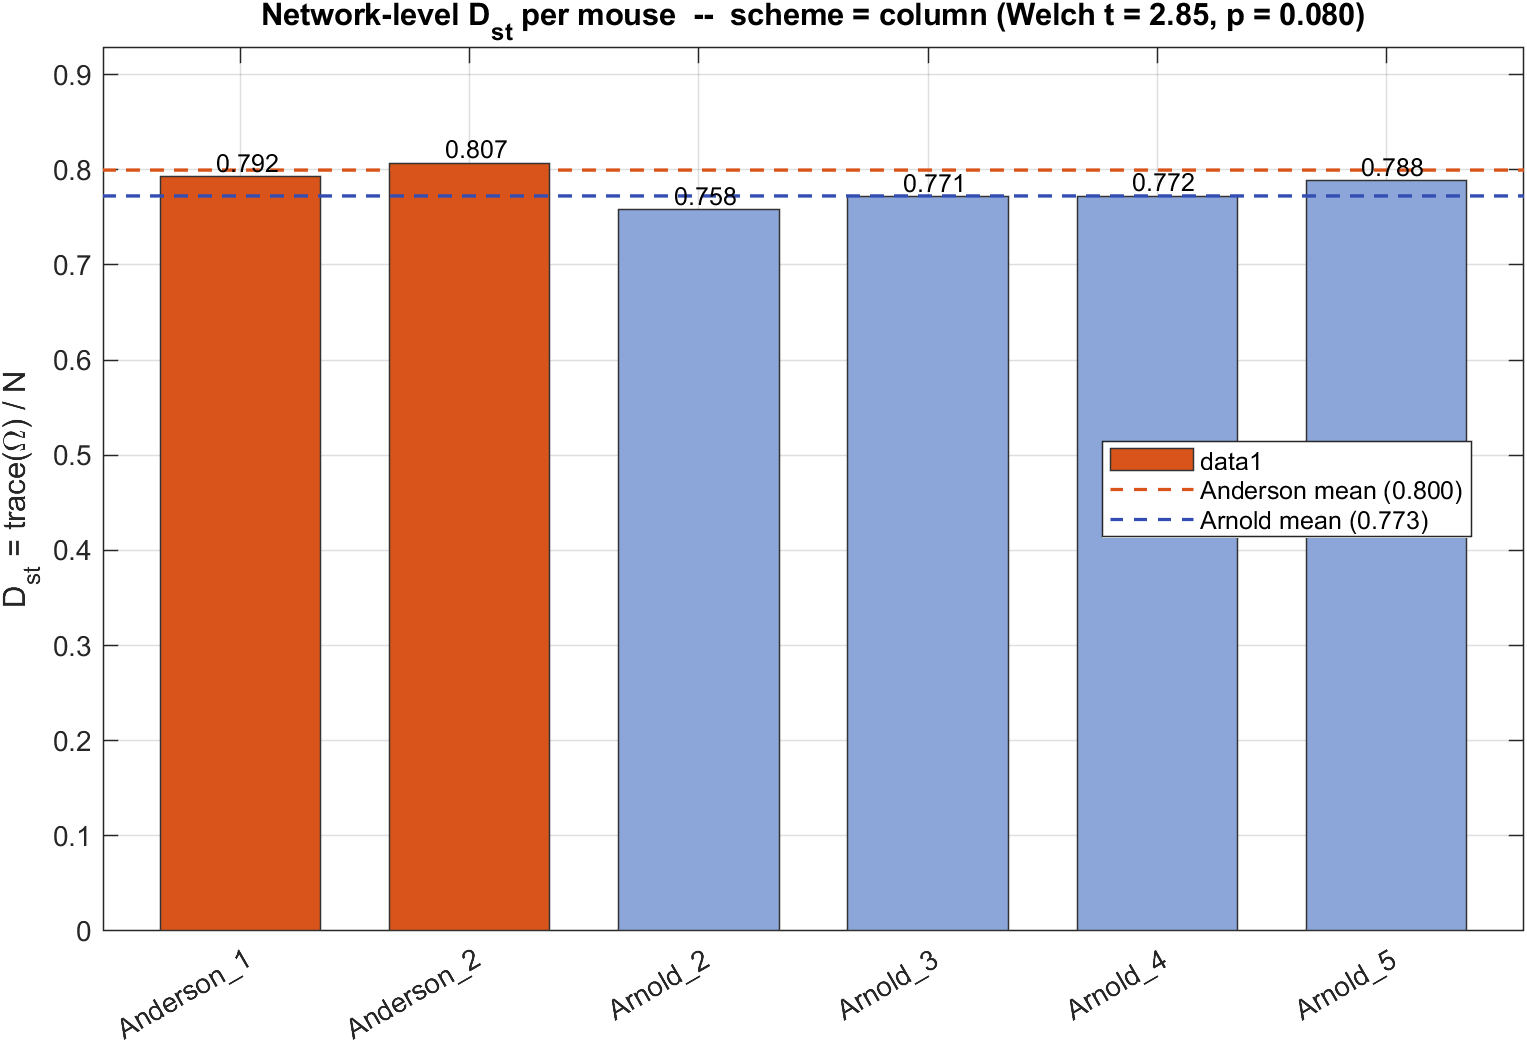
\includegraphics[width=0.78\linewidth]{fig_dst_column.png}
\caption{Network-level $\Dst=\mathrm{trace}(\Omega)/N$ per mouse, \texttt{column} scheme. Case
(\textsc{Anderson}, orange) and control (\textsc{Arnold}, blue) ranges do not overlap (min case
$0.792>$ max control $0.788$); dashed lines are cohort means ($0.800$ vs $0.773$). Welch $t=2.85$,
$p=0.080$.}
\label{fig:dst}
\end{figure}

\subsection{A structural centrality reproduces a dynamics-based ground truth}
Under the Epileptor (\texttt{tvb}) scheme, per-region stability centrality and the independently
computed critical excitability $\xcrit$ trace a near one-to-one decreasing curve in both case mice
(Fig.~\ref{fig:x0}): regions with the highest $\Dto$ are exactly those that destabilise the network at
the lowest added excitability---i.e.\ those closest to their own seizure threshold. The same regions
sit atop the curve in \textsc{Anderson\_1} and \textsc{Anderson\_2}, and the consensus top regions are
high-connectivity thalamic and basal-ganglia nuclei. This reproduces the single-patient result of
\citet{liao_thesis2026} across animals: a purely \emph{structural} score recovers a \emph{dynamical}
ground truth, and it does so consistently, which validates the method itself before any
epilepsy-specific contrast. Because $\xcrit$ is read from the nonlinear Epileptor bifurcation while
$\Dto$ is read from the linear covariance, the two derivations are methodologically independent;
their agreement across both case mice is strong evidence that $D$ is consistent with a biologically
meaningful network property rather than an artefact of either route.

\begin{figure}[H]
\centering
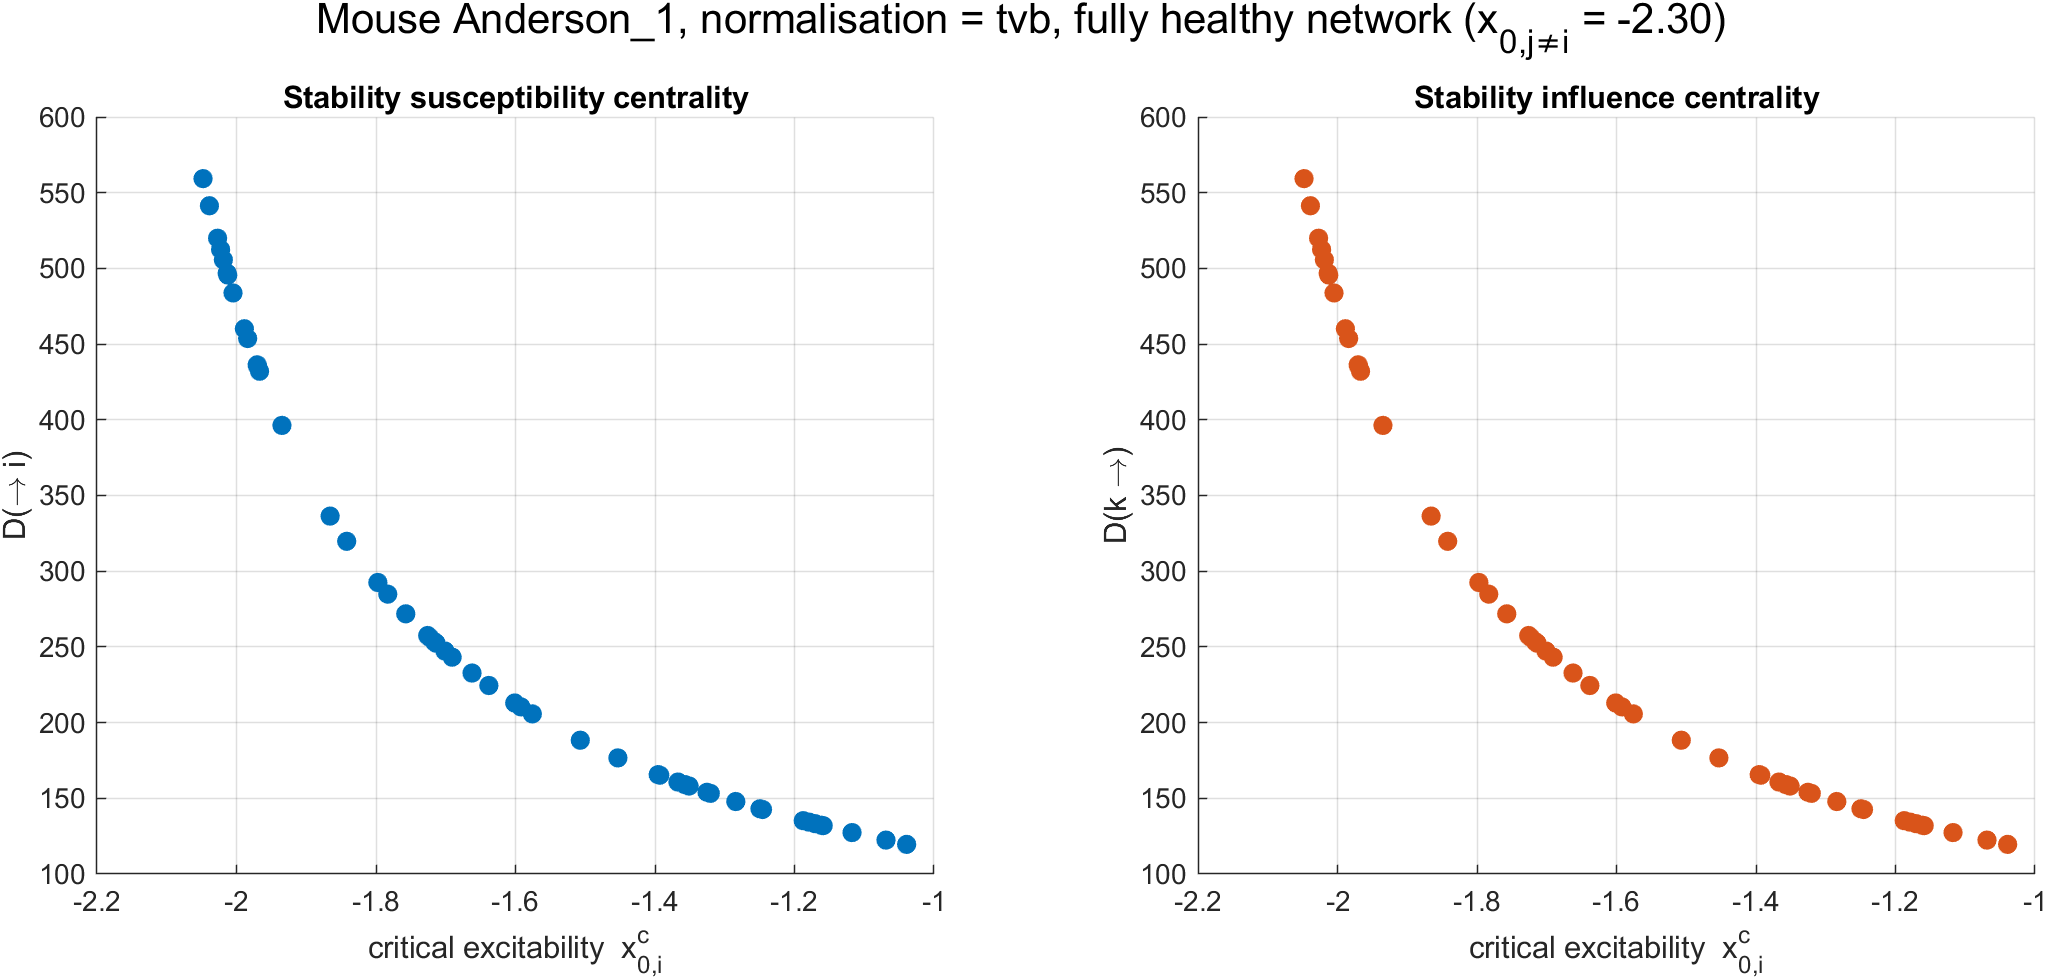
\includegraphics[width=0.92\linewidth]{fig_x0_anderson1_tvb.png}
\caption{Per-region stability centrality vs.\ critical excitability $\xcrit$ for \textsc{Anderson\_1}
(\texttt{tvb}). Left: susceptibility $\Dto$; right: influence $\Dfrom$ (identical under the symmetric
scheme). High centrality corresponds to low $\xcrit$, i.e.\ proximity to the seizure threshold. The
relationship replicates in \textsc{Anderson\_2}.}
\label{fig:x0}
\end{figure}

\subsection{Whether $D$ adds information depends on the normalisation}
Under the symmetry-preserving normalisations (\texttt{parkes}, \texttt{tvb}), the node-level
centralities prove largely redundant, collapsing onto a single ranking. Across the cohort the
walk-based measures---weighted in/out-degree, eigenvector centrality, PageRank, Katz,
self-communicability, and the stability susceptibility $\Dto$---agree at cohort-mean Spearman
$\rho\ge 0.98$ (median $0.99$); even shortest-path closeness tracks them at $\rho\approx 0.96$,
leaving betweenness centrality \citep{rubinov2010} as the only meaningful departure
($\rho\approx 0.79$ against $\Dto$). Two mechanisms drive the collapse. \emph{First}, symmetry of the
coupling matrix forces the two directed stability centralities to coincide exactly: the
susceptibility $\Dto$ and the influence $\Dfrom$ are then read from one and the same stationary
covariance $\Omega=\tfrac{\zeta^2}{2}(I-C)^{-1}$ \citep{liao_lizier2026}. \emph{Second}, the
connectomes carry a clear spectral gap---the ratio $\lambda_2/\lambda_{\max}$ lies between $0.49$ and
$0.68$ across the six mice---so the leading eigenvalue is well separated from the rest. In the
spectral form $\Omega=\tfrac{\zeta^2}{2}\sum_k(1-\lambda_k)^{-1}q_k q_k^{\top}$ the leading mode
$q_1$ then dominates the node-to-node variation of $\Omega$, and because every walk-based measure is
a weighted sum over powers of $C$ \citep{schwarze2021} all inherit that dominant-mode profile and
reduce to the leading eigenvector---that is, to eigenvector centrality (indeed $\Dto$ correlates with
it at $\rho\approx 0.997$). The system moreover sits just \emph{below} the stability boundary
($\rhoC\approx0.99999$ under \texttt{parkes}), which weights $q_1$ by $(1-\lambda_{\max})^{-1}$---more than
four orders of magnitude above the next mode---so that the leading mode accounts for $\approx 99.9\%$
of $\mathrm{trace}(\Omega)$ and $\Omega$ is, for ranking purposes, effectively of rank one.
Betweenness escapes not merely because it is path-based---closeness is too, yet still collapses---but
because it scores how often a node bridges shortest paths between \emph{other} regions, a bottleneck
role (here flagging white-matter, CSF and cranial-nerve nodes) orthogonal to dominant-mode magnitude.

The redundancy is therefore a deterministic consequence of symmetry and spectral structure, not an
artefact of the small sample size, and it cannot be relieved by rescaling the coupling strength:
scaling keeps $C$ symmetric, so $\Dto\equiv\Dfrom$ exactly, and preserves both the eigenvectors and
the gap ratio $\lambda_2/\lambda_{\max}$, leaving $\rho(\Dto,\mathrm{EC})\ge 0.9996$ even as $\rhoC$
is lowered to $\approx 0.99$ \citep{parkes2024}. It is relieved only by breaking the matrix symmetry
(Fig.~\ref{fig:corr}): under the \texttt{column} normalisation the two stability centralities
decouple ($\rho\approx 0.75$), the in-style measures sign-flip against $\Dto$ ($\rho\approx -0.78$),
and the susceptibility's correlation with the out-eigenvector centrality falls to $\rho\approx 0.76$,
recovering the independent directed signal on which the region-level comparison of susceptibility and
influence depends. This is precisely the symmetric$\to$asymmetric transition reported by
\citet{liao_lizier2026}, here reproduced on real brain networks.

\begin{figure}[H]
\centering
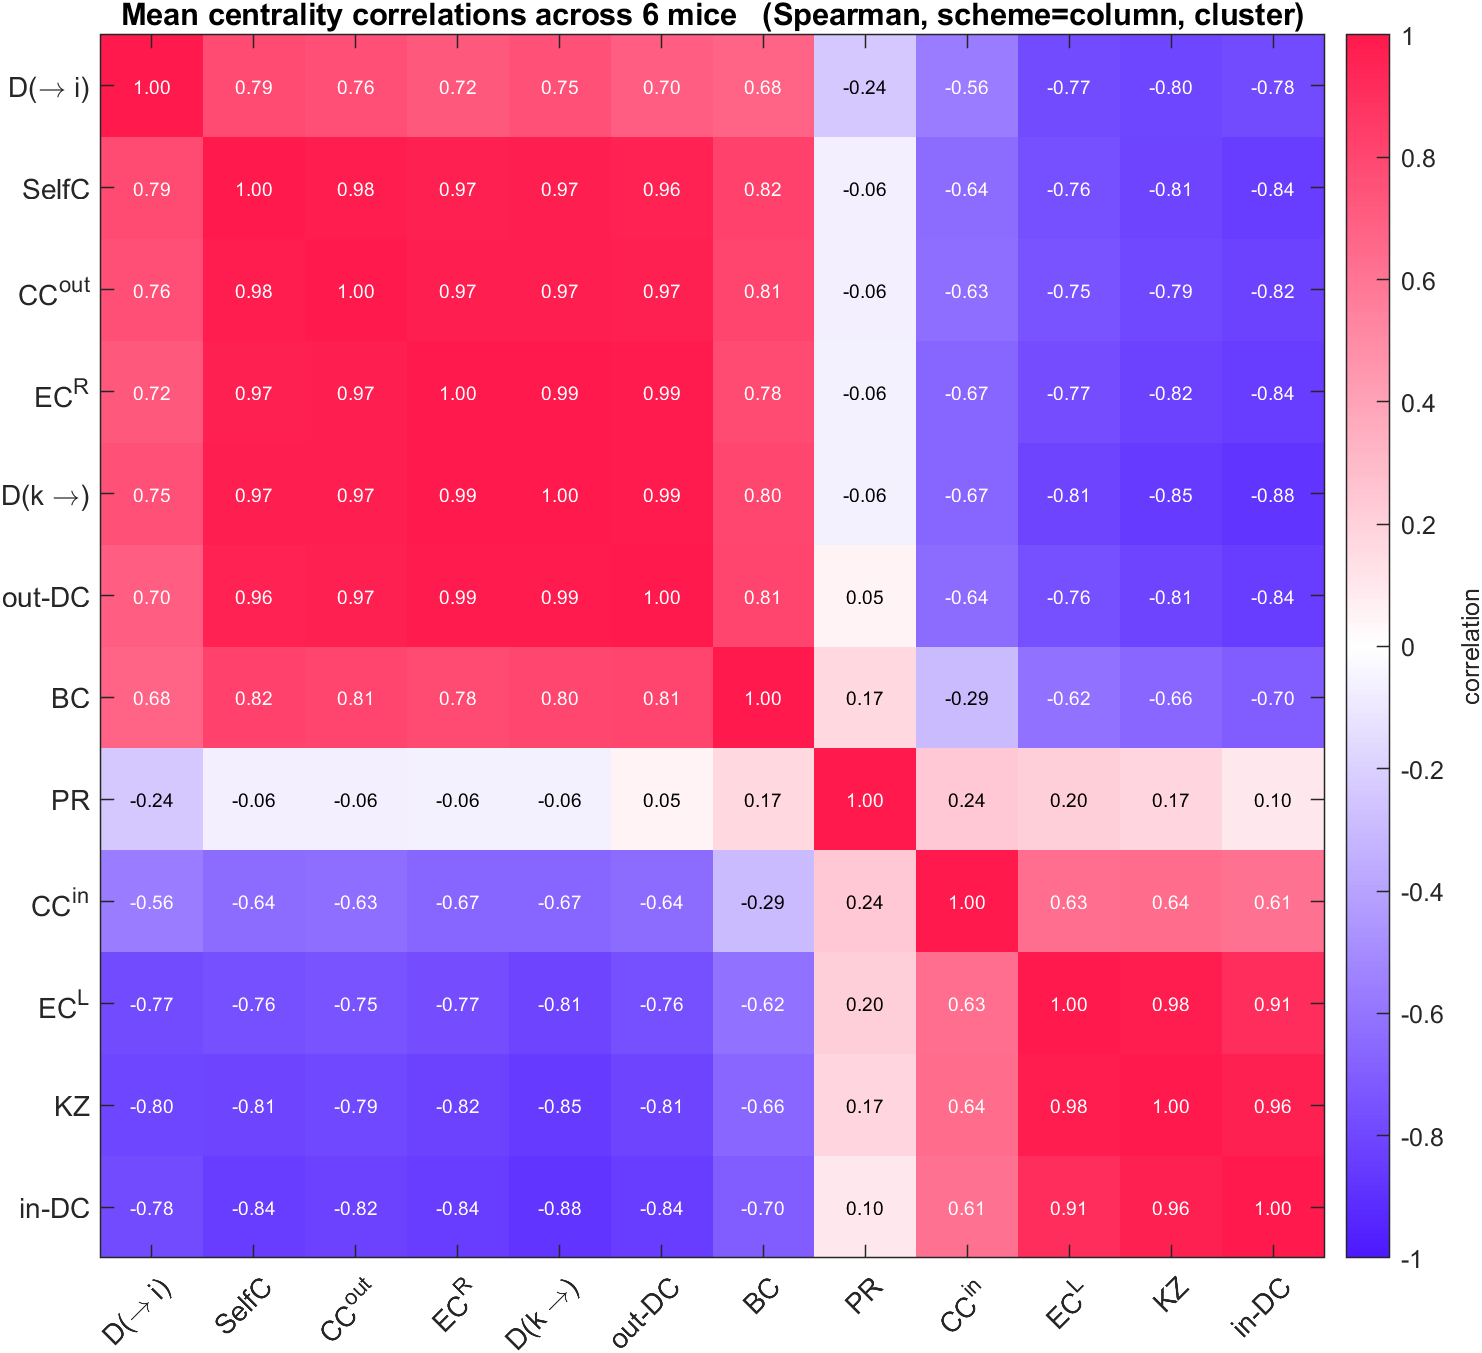
\includegraphics[width=0.66\linewidth]{fig_corr_mean_column.png}
\caption{Cohort-mean Spearman correlation of $\Dto$ and $\Dfrom$ with ten classical centralities,
\texttt{column} scheme. In-style measures anti-correlate with $\Dto$ and the two stability
centralities decouple ($\rho\approx 0.75$), confirming $D$ carries independent per-node information
only when symmetry is broken.}
\label{fig:corr}
\end{figure}

\subsection{Per-region outliers flag epileptologically interpretable structures}
Contrasting each case mouse against the four-control band under \texttt{column} flags
Bonferroni-significant susceptibility excesses concentrated in limbic and sensorimotor cortex
(Fig.~\ref{fig:susc}, Fig.~\ref{fig:outliers}). Two regions are \emph{cohort-robust}, flagged in both
case mice: \textbf{gustatory cortex (L)} ($+20.6\%$, $z=7.9$ in \textsc{Anderson\_2}; $+10.5\%$, $z=4.0$
in \textsc{Anderson\_1}) and the \textbf{hippocampal formation} ($+9.9\%$, $z=6.7$ on the L side of
\textsc{Anderson\_2}; $+6.6\%$, $z=5.4$ on the R side of \textsc{Anderson\_1}). Single-mouse signals
add somatosensory cortex ($+12.3\%$), temporal-association cortex ($+7.2\%$) and basal-ganglia
striatum ($+5.5\%$). Mesial temporal lobe epilepsy with hippocampal sclerosis is a canonical focal epilepsy syndrome
\citep{wieser2004}, so the hippocampal formation's appearance as a cohort-robust outlier is
biologically reassuring. By contrast, classical betweenness on the same
mice flags white-matter, CSF and cranial-nerve nodes---anatomical artefacts of the tractography rather
than epileptogenic tissue---underlining that a dynamics-based centrality targets more plausible
structures than a purely topological one.

\begin{figure}[H]
\centering
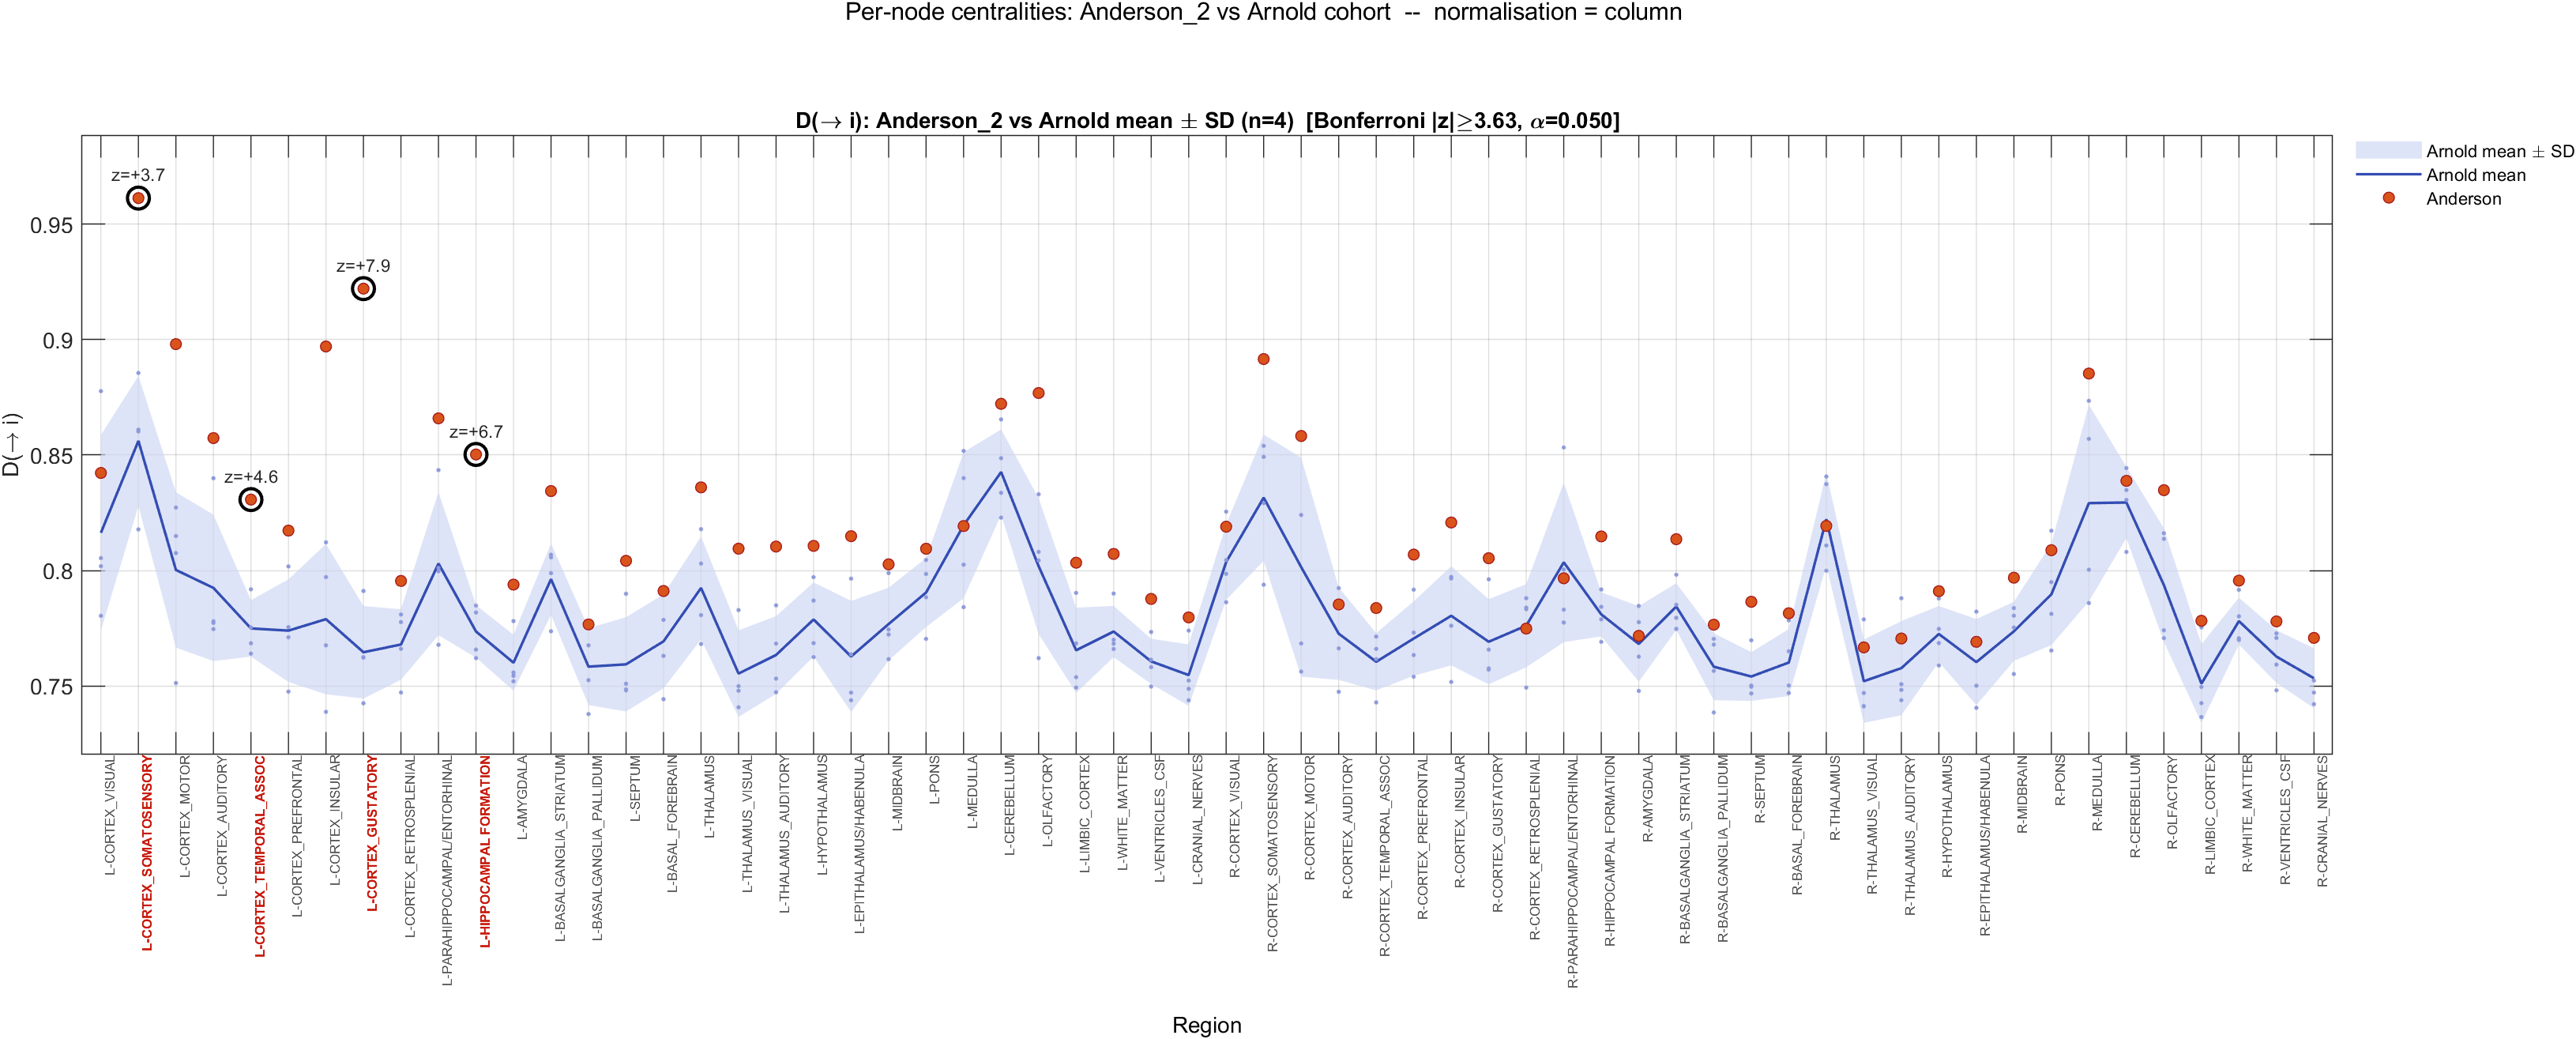
\includegraphics[width=0.86\linewidth]{fig_susc_anderson2_column.png}
\caption{Per-region susceptibility $\Dto$ for \textsc{Anderson\_2} (red) against the four-control band
(mean\,$\pm$\,SD), \texttt{column} scheme. Ringed, bold-labelled nodes are Bonferroni-significant.
Limbic and sensory cortical regions exceed the control band.}
\label{fig:susc}
\end{figure}

\begin{figure}[H]
\centering
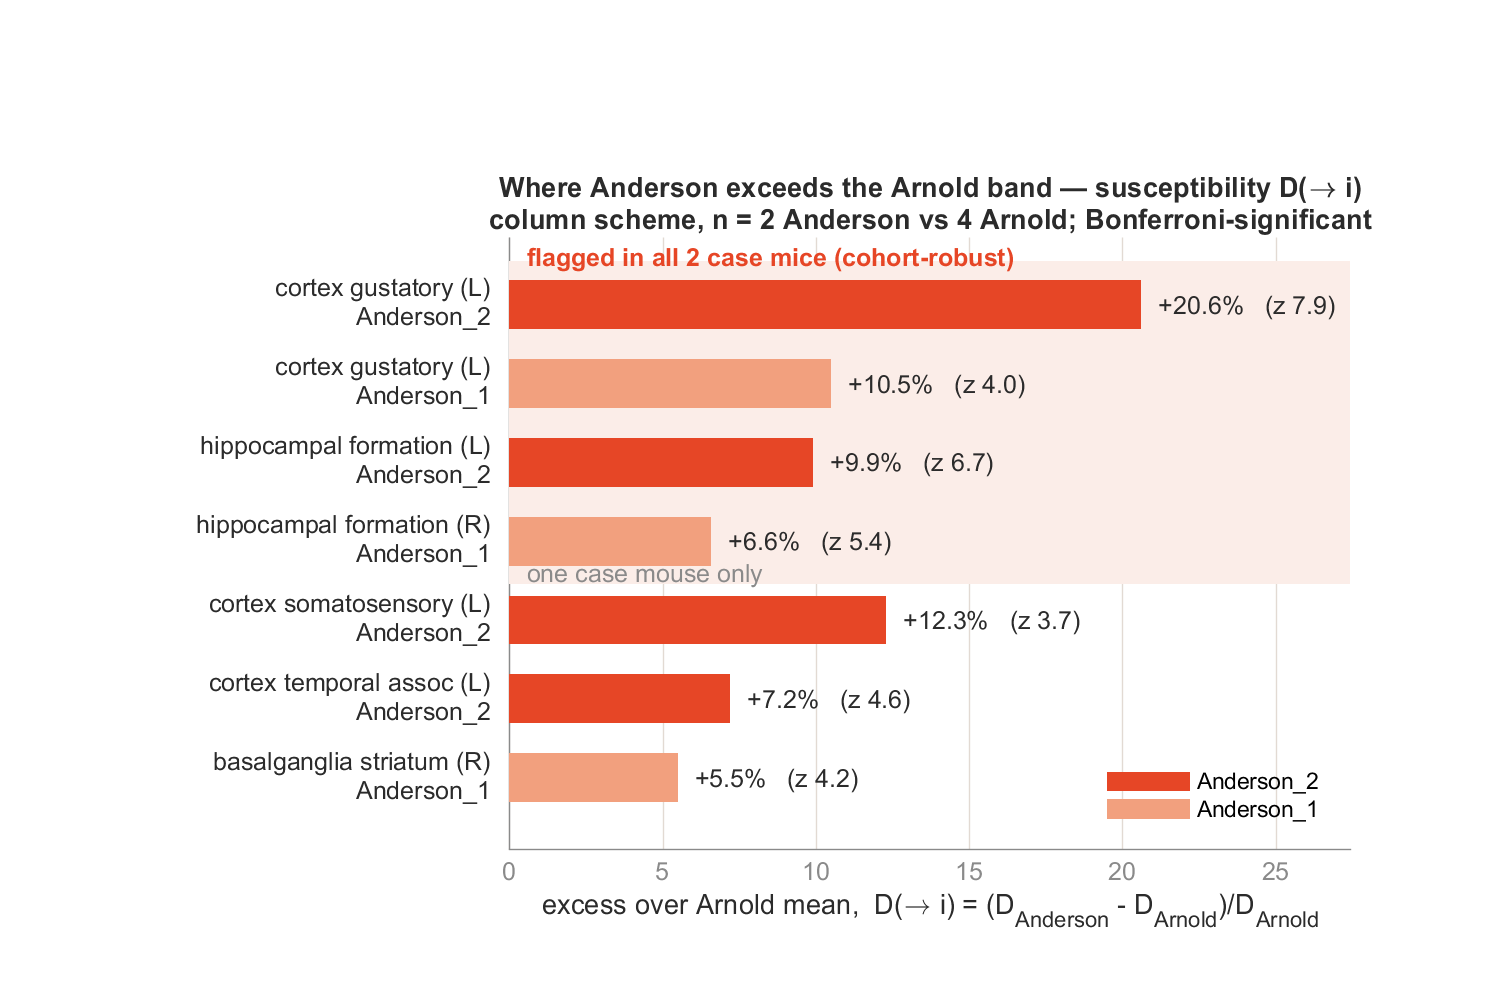
\includegraphics[width=0.74\linewidth]{fig_region_susc_outliers.png}
\caption{All Bonferroni-significant $\Dto$ excesses over the control mean (\texttt{column}). Gustatory
cortex (L) and hippocampal formation flag in both case mice (shaded, ``cohort-robust''); remaining
rows are single-mouse signals.}
\label{fig:outliers}
\end{figure}

\subsection{A left--right asymmetry signal beyond the single-patient study}
Laterality requires a cohort to define and is therefore absent from the thesis. At the cohort level,
the case mice show a significant systematic side bias in $\mathrm{LI}_{\mathrm{norm}}$ under every
scheme (sign-rank $p<0.002$), toward the \texttt{L} side under \texttt{column}/\texttt{parkes} and the
\texttt{R} side under \texttt{tvb}; controls are largely silent. Per homotopic pair, the
group-level Welch test flags the parahippocampal/entorhinal influence pair under \texttt{column}
($t=4.50$, $p_{\mathrm{bonf}}=0.021$) and the white-matter pair under \texttt{tvb}
($p_{\mathrm{bonf}}=0.034$). The per-case view (Fig.~\ref{fig:lr}) shows excess left-side
\emph{influence} at olfactory ($+1.52$, $z=4.9$) and motor cortex ($+0.75$, $z=6.3$) in
\textsc{Anderson\_2}; no homotopic pair survives correction in \textsc{Anderson\_1}, so this is
suggestive rather than replicated. The limbic--thalamic flavour of these effects is consistent with the clinical relevance of left--right lateralisation in
temporal-lobe epilepsy \citep{cendes1997,li2000}, with the caveat that the side labels are nominal. Surfacing a hemispheric
signal at all is a cohort-only contribution beyond the single-patient study; at $n=2$ cases, though,
it is a lead to pursue with directed inputs rather than a settled asymmetry.

\begin{figure}[H]
\centering
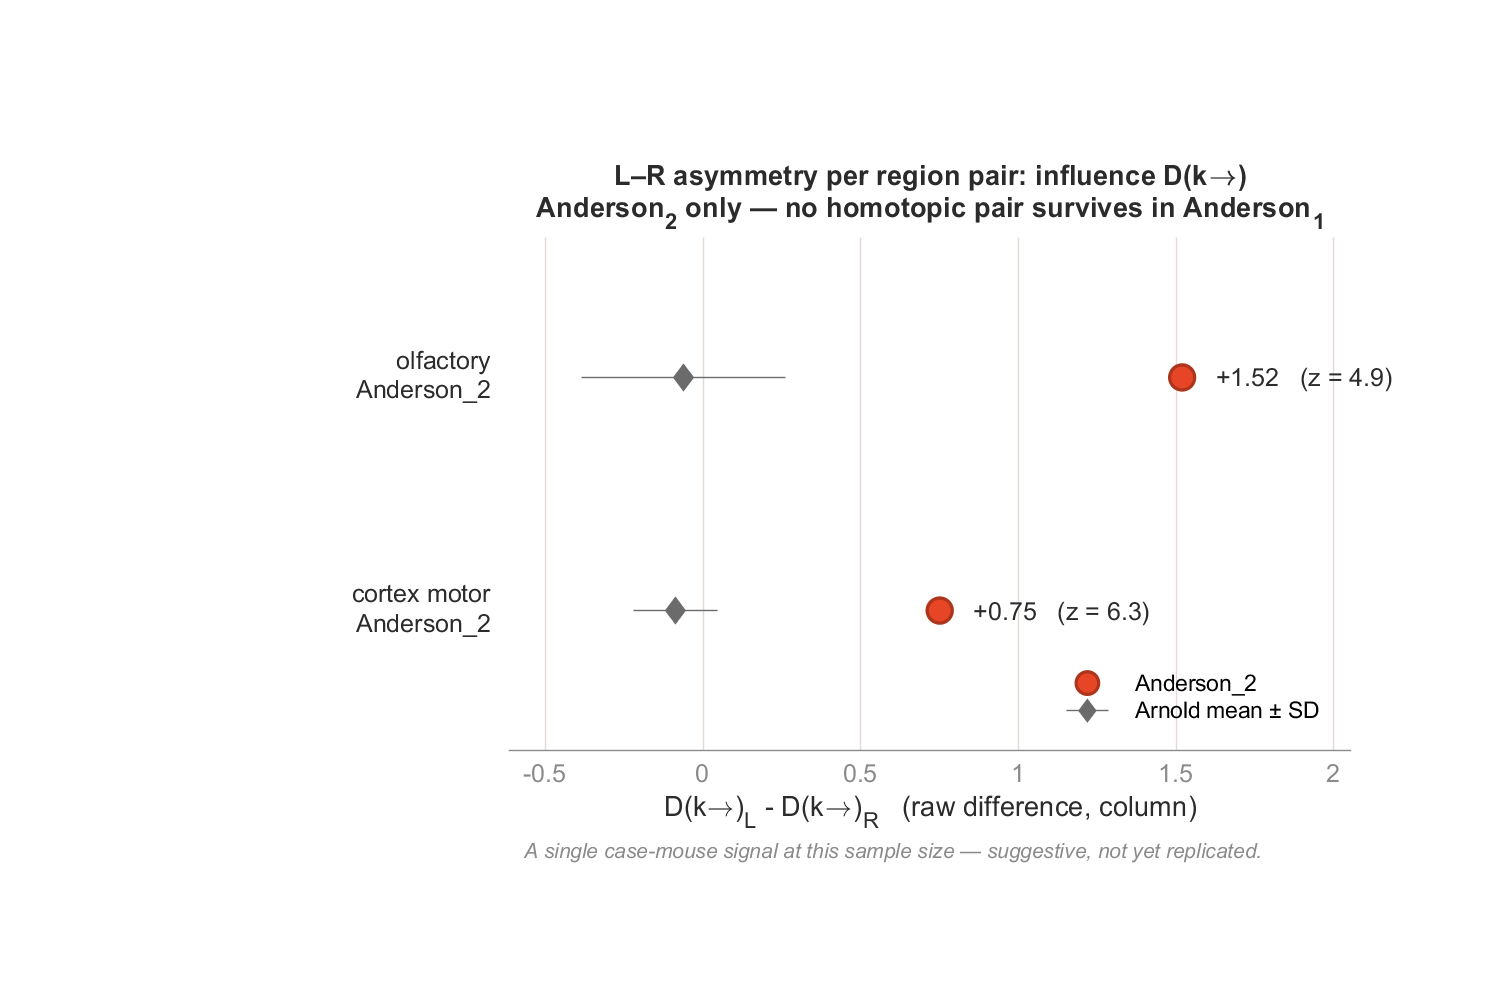
\includegraphics[width=0.72\linewidth]{fig_lr_influence_outliers.png}
\caption{Left--right asymmetry of influence $\Dfrom$ per homotopic pair, \texttt{column}. Case value
$L-R$ (red) vs.\ the control band (grey, mean\,$\pm$\,SD). \textsc{Anderson\_2} shows excess left-side
influence at olfactory and motor cortex; no pair survives correction in \textsc{Anderson\_1}.}
\label{fig:lr}
\end{figure}

% ===========================================================================
\section{Limitations and future work}
\label{sec:limits}
% ===========================================================================
The cohort is small: $n=2$ case vs $4$ control. The $\Dst$ separation is therefore a hypothesis
($p=0.080$) until replicated, and at this sample size only the largest effects clear Bonferroni
correction---motor, amygdala and the laterality pairs sit near or below threshold for reasons of
statistical power, not biology. We mitigate this by reporting effect sizes alongside $z$-scores and by
leaning on the largest, replicated effects (gustatory cortex, hippocampal formation). The headline
findings live in the \texttt{column} scheme; \texttt{tvb} and \texttt{parkes} tell a flatter story, so
the conclusions are explicitly conditional on a modelling choice that we state rather than hide.
Finally, the input is symmetric structural connectivity, so the in/out asymmetry that makes the
centralities informative is imposed by normalisation rather than measured from directed interactions.

The natural next steps are: larger cohorts per strain to convert the $\Dst$ separation from hypothesis
to result; \emph{directed} effective connectivity (e.g.\ transfer entropy \citep{vicente2011} or DCM \citep{friston2003}) as input, so that
$\Dto$ and $\Dfrom$ separate for a measured rather than imposed reason; and per-node critical-%
excitability thresholds computed under the primary \texttt{column} scheme, bridging the structural
centralities and the dynamical ground truth within a single normalisation.

% ===========================================================================
\section{Conclusion}
% ===========================================================================
$\Dst$ gives a graded, full-spectrum stability signal where the dominant eigenvalue gives only a
yes/no answer, and its two node-level centralities rank regions by a structural stability proxy
plausibly related to epileptogenic vulnerability. On real
mouse connectomes those rankings match an independent Epileptor-derived threshold and recover known
seizure-onset biology; at the network level, $\Dst$ shows non-overlapping cohort ranges in this small sample under \texttt{column} normalisation and
reveals a new hemispheric-asymmetry signal absent from the single-patient study it builds on.
Crucially, the framework's usefulness on structural data hinges on breaking the connectome's symmetry,
not on tuning constants. With larger cohorts and directed inputs, deviation-from-stability centralities
are a promising structural screening tool for prioritising candidate epileptogenic regions.

% ===========================================================================
\begin{thebibliography}{9}
\small
\bibitem[Cendes et al.(1997)]{cendes1997} Cendes, F., Caramanos, Z., Andermann, F., Dubeau, F., \& Arnold, D.~L. (1997). Proton magnetic resonance spectroscopic imaging and magnetic resonance imaging volumetry in the lateralization of temporal lobe epilepsy: a series of 100 patients. \emph{Annals of Neurology}, 42(5), 737--746.

\bibitem[Fiest et al.(2017)]{fiest2017} Fiest, K.~M., et al. (2017). Prevalence and incidence of
epilepsy: a systematic review and meta-analysis of international studies. \emph{Neurology},
88(3), 296--303.

\bibitem[Friston et al.(2003)]{friston2003} Friston, K.~J., Harrison, L., \& Penny, W. (2003). Dynamic causal modelling. \emph{NeuroImage}, 19(4), 1273--1302.

\bibitem[Jirsa et al.(2014)]{jirsa2014} Jirsa, V.~K., Stacey, W.~C., Quilichini, P.~P., Ivanov, A.~I., \& Bernard, C. (2014). On the nature
of seizure dynamics. \emph{Brain}, 137(8), 2210--2230.

\bibitem[Jirsa et al.(2017)]{jirsa2017} Jirsa, V.~K., et al. (2017). The Virtual Epileptic Patient:
individualized whole-brain models of epilepsy spread. \emph{NeuroImage}, 145, 377--388.

\bibitem[Li et al.(2000)]{li2000} Li, L.~M., Caramanos, Z., Cendes, F., Andermann, F., Antel, S.~B., Dubeau, F., \& Arnold, D.~L. (2000). Lateralization of temporal lobe epilepsy (TLE) and discrimination of TLE from extra-TLE using pattern analysis of magnetic resonance spectroscopic and volumetric data. \emph{Epilepsia}, 41(7), 832--842.

\bibitem[Liao(2026)]{liao_thesis2026} Liao, J. (2026). \emph{Stability of Brain Networks in Epilepsy}, Ch.~4. Unpublished MSc thesis, The University of Sydney.

\bibitem[Liao \& Lizier(2026)]{liao_lizier2026} Liao, J., \& Lizier, J.~T. (2026). Directly
quantifying deviation from stability for linear dynamical systems on networks. Unpublished manuscript, School of
Computer Science \& Centre for Complex Systems, The University of Sydney.

\bibitem[Maier-Hein et al.(2017)]{maierhein2017} Maier-Hein, K.~H., et al. (2017). The challenge of mapping the human connectome based on diffusion tractography. \emph{Nature Communications}, 8, 1349.

\bibitem[Parkes et al.(2024)]{parkes2024} Parkes, L., Kim, J.~Z., Stiso, J., et al. (2024). A network
control theory pipeline for studying the dynamics of the structural connectome. \emph{Nature
Protocols}, 19, 3721--3749.

\bibitem[Rosenow \& L\"uders(2001)]{rosenow2001} Rosenow, F., \& L\"uders, H. (2001). Presurgical evaluation of epilepsy. \emph{Brain}, 124(9), 1683--1700.

\bibitem[Rubinov \& Sporns(2010)]{rubinov2010} Rubinov, M., \& Sporns, O. (2010). Complex network
measures of brain connectivity: uses and interpretations. \emph{NeuroImage}, 52(3), 1059--1069.

\bibitem[Sanz Leon et al.(2013)]{sanzleon2013} Sanz Leon, P., et al. (2013). The Virtual Brain: a
simulator of primate brain network dynamics. \emph{Frontiers in Neuroinformatics}, 7, 10.

\bibitem[Schwarze \& Porter(2021)]{schwarze2021} Schwarze, A.~C., \& Porter, M.~A. (2021). Motifs for
processes on networks. \emph{SIAM Journal on Applied Dynamical Systems}, 20(4), 2516--2557.

\bibitem[Vicente et al.(2011)]{vicente2011} Vicente, R., Wibral, M., Lindner, M., \& Pipa, G. (2011). Transfer entropy---a model-free measure of effective connectivity for the neurosciences. \emph{Journal of Computational Neuroscience}, 30(1), 45--67.

\bibitem[Wieser(2004)]{wieser2004} Wieser, H.~G. (2004). ILAE Commission Report. Mesial temporal lobe epilepsy with hippocampal sclerosis. \emph{Epilepsia}, 45(6), 695--714.
\end{thebibliography}

% ===========================================================================
\appendix
\section{Acknowledgement of generative-AI use}
In line with the University of Sydney's policy on generative AI, the author used Anthropic Claude
(Opus 4.x) for language editing, structural suggestions, and assembling pre-computed result figures
into report form, and AI-assisted coding tools (Cursor, Claude Code) for code-completion support
while developing some of the MATLAB analysis scripts and their documentation. These tools were
\emph{not} used to choose the research question, define the methodology, select parameters, decide
which results to report, perform the statistical interpretation, or generate unsupported scientific
claims. All scientific design, parameter choices, result validation, and interpretation were
performed by the author, who takes full responsibility for the submitted work and confirms it is
their own, prepared in accordance with University guidelines.

\section{Reproducibility}
\label{app:repro}
All results derive from three configuration-driven pipeline runs (\texttt{column}, \texttt{parkes},
\texttt{tvb}) over the six-mouse cohort, executed in MATLAB R2024b. Each run records its full parameter
set and a step-by-step manifest, and writes per-mouse stability results, cohort summaries, strain
contrasts, laterality tests, and network-$\Dst$ tables. Numerical settings: continuous-time OU
dynamics, covariance power-series cap $10^8$; Epileptor $\tau_0=6667$, healthy $x_0=-2.3$, $\xcrit$
bisection tolerance $10^{-4}$; Bonferroni $\alpha=0.05$.

\section{Full result figures }
\label{app:figures}
This appendix reproduces \emph{every} figure generated by the three configuration-driven
pipeline runs of the latest experiment configuration (\texttt{column}, \texttt{parkes}, \texttt{tvb}; run 2026-05-27)
over the six-mouse cohort. A representative subset appears in the main text; the complete set is
collected here for reference. Within each panel grid the two \textsc{Anderson} case mice precede the
four \textsc{Arnold} controls.

\subsection{Network-level \texorpdfstring{$\Dst$}{Dst} across the cohort}
\begin{figure}[H]\centering
\begin{subfigure}{0.32\textwidth}\centering
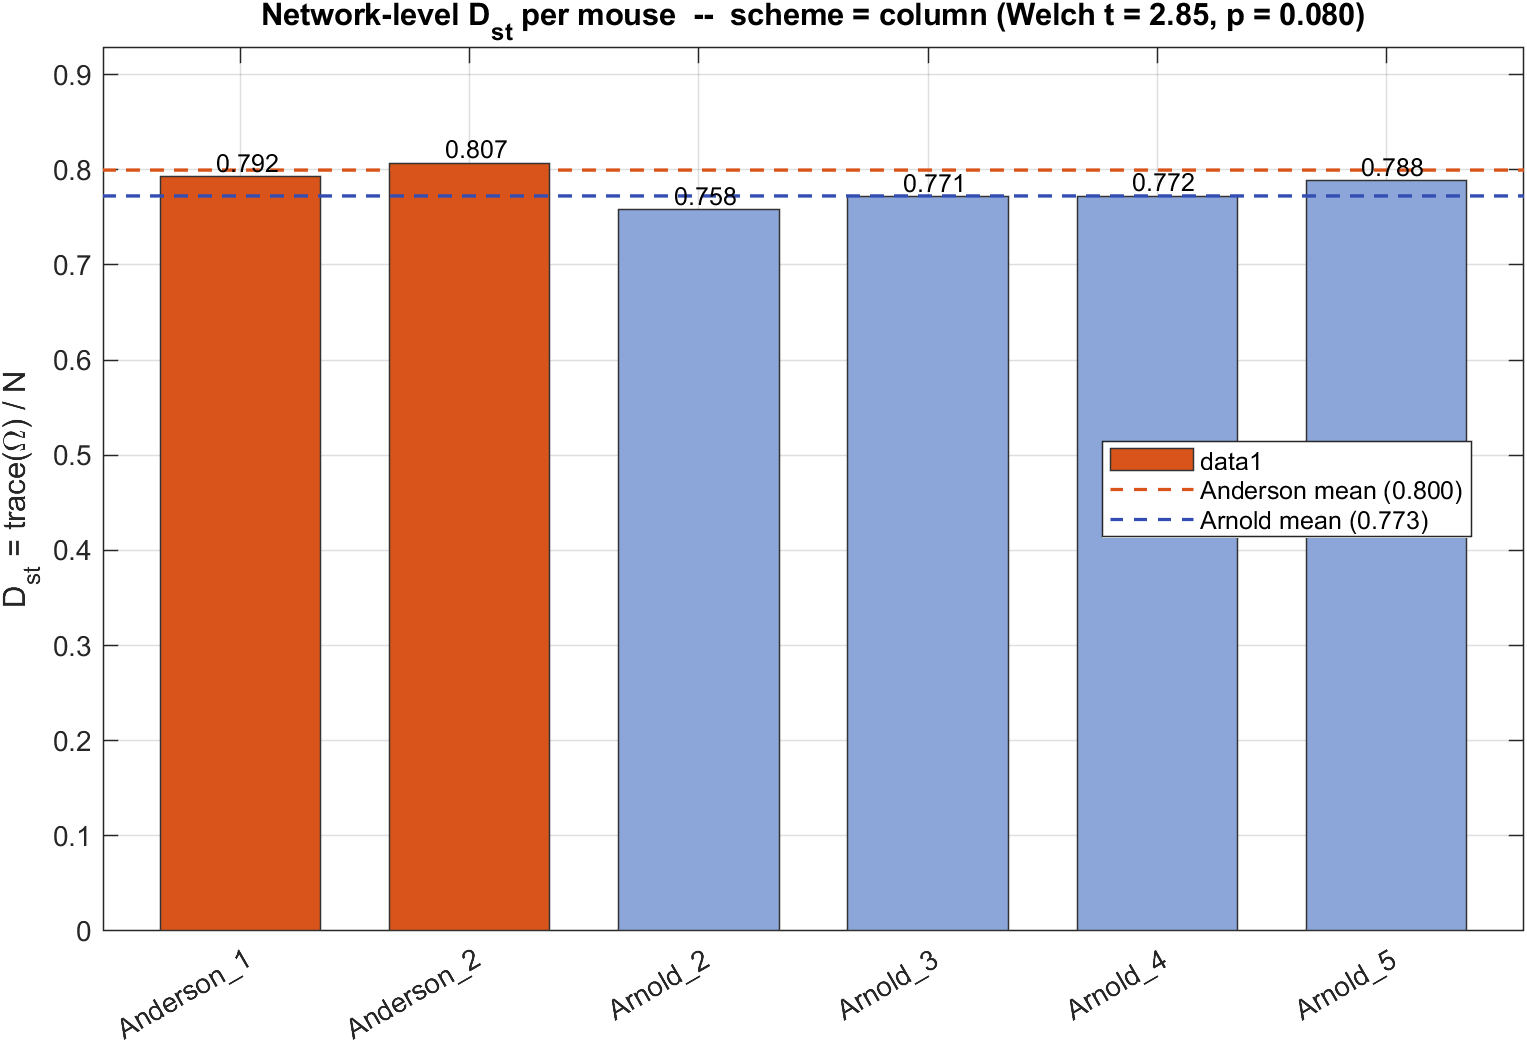
\includegraphics[width=\linewidth]{appendix/D_st_cohort_column.png}
\caption{\texttt{column}}
\end{subfigure}\hfill
\begin{subfigure}{0.32\textwidth}\centering
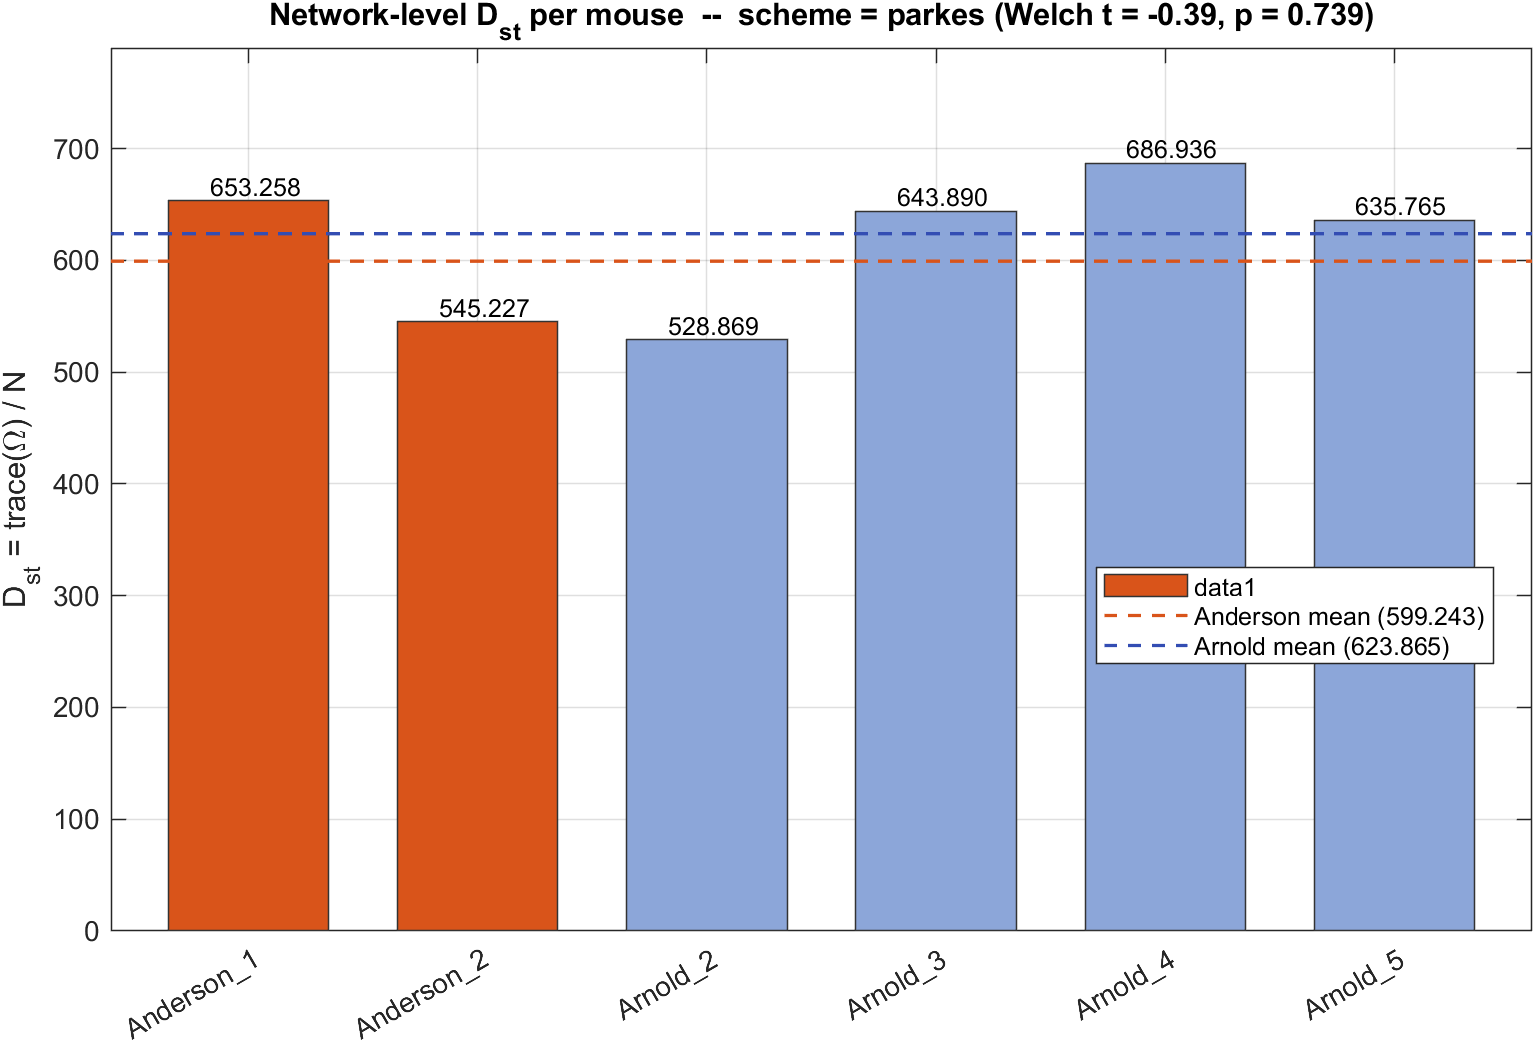
\includegraphics[width=\linewidth]{appendix/D_st_cohort_parkes.png}
\caption{\texttt{parkes}}
\end{subfigure}\hfill
\begin{subfigure}{0.32\textwidth}\centering
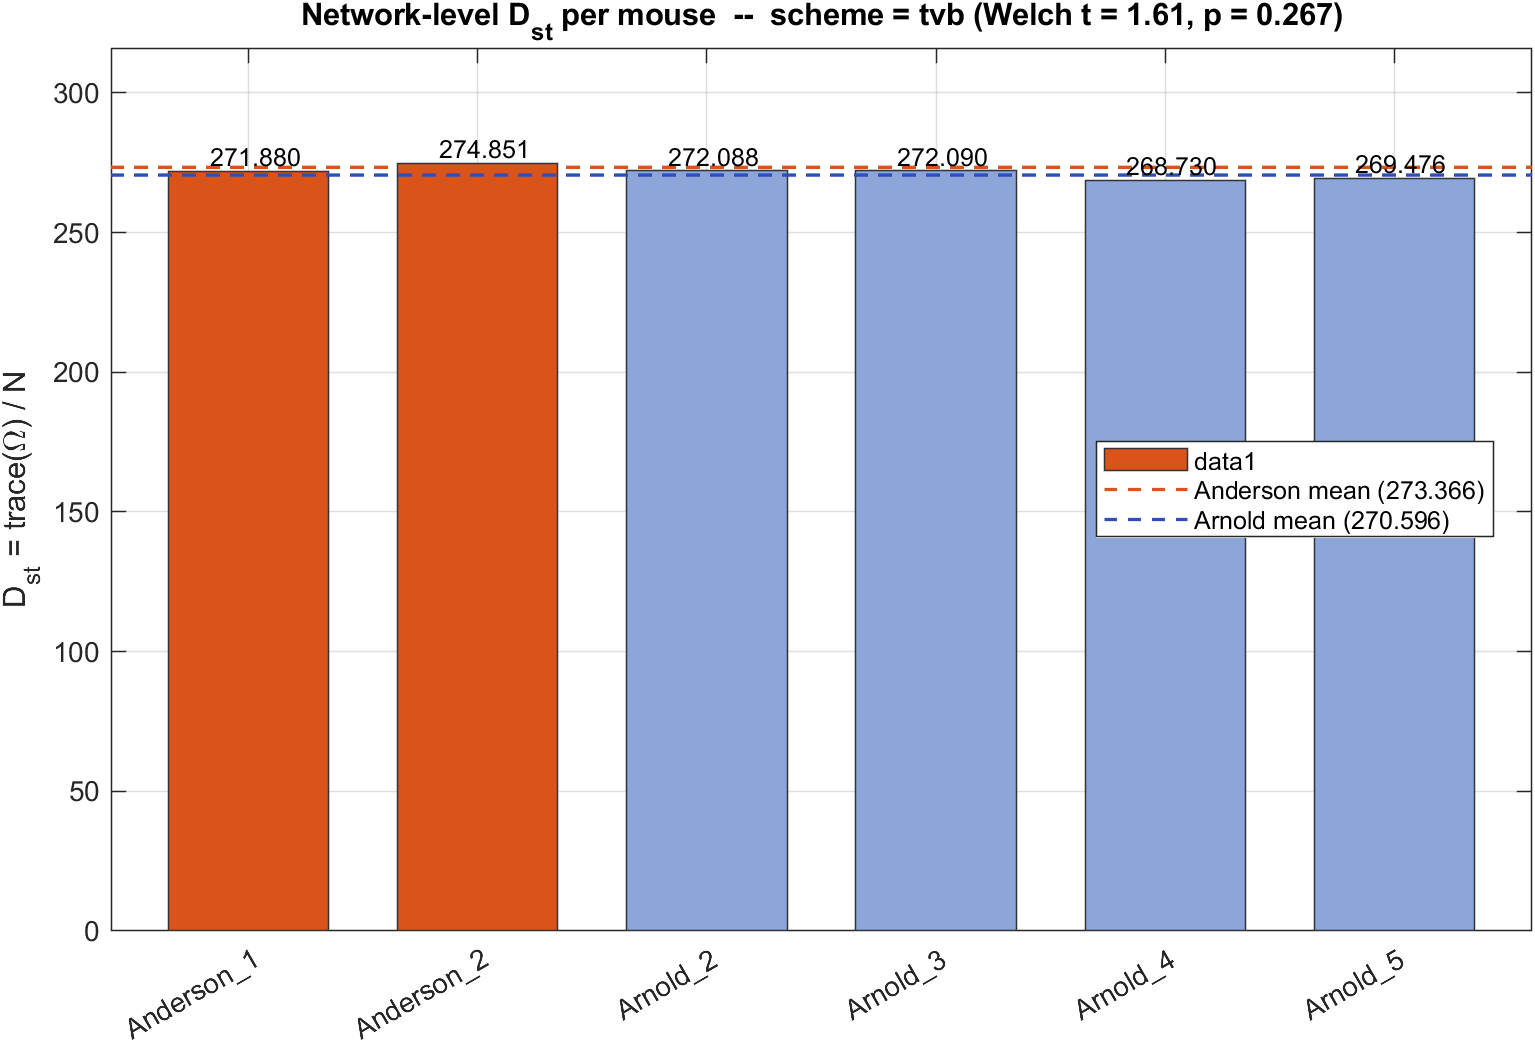
\includegraphics[width=\linewidth]{appendix/D_st_cohort_tvb.png}
\caption{\texttt{tvb}}
\end{subfigure}\hfill
\caption{Per-mouse network $\Dst=\mathrm{trace}(\Omega)/N$ for each normalisation scheme. Only \texttt{column} separates the strains; under \texttt{parkes}/\texttt{tvb} the cohort ranges overlap.}
\end{figure}

\subsection{Per-region stability centralities}
\begin{figure}[H]\centering
\begin{subfigure}{0.32\textwidth}\centering
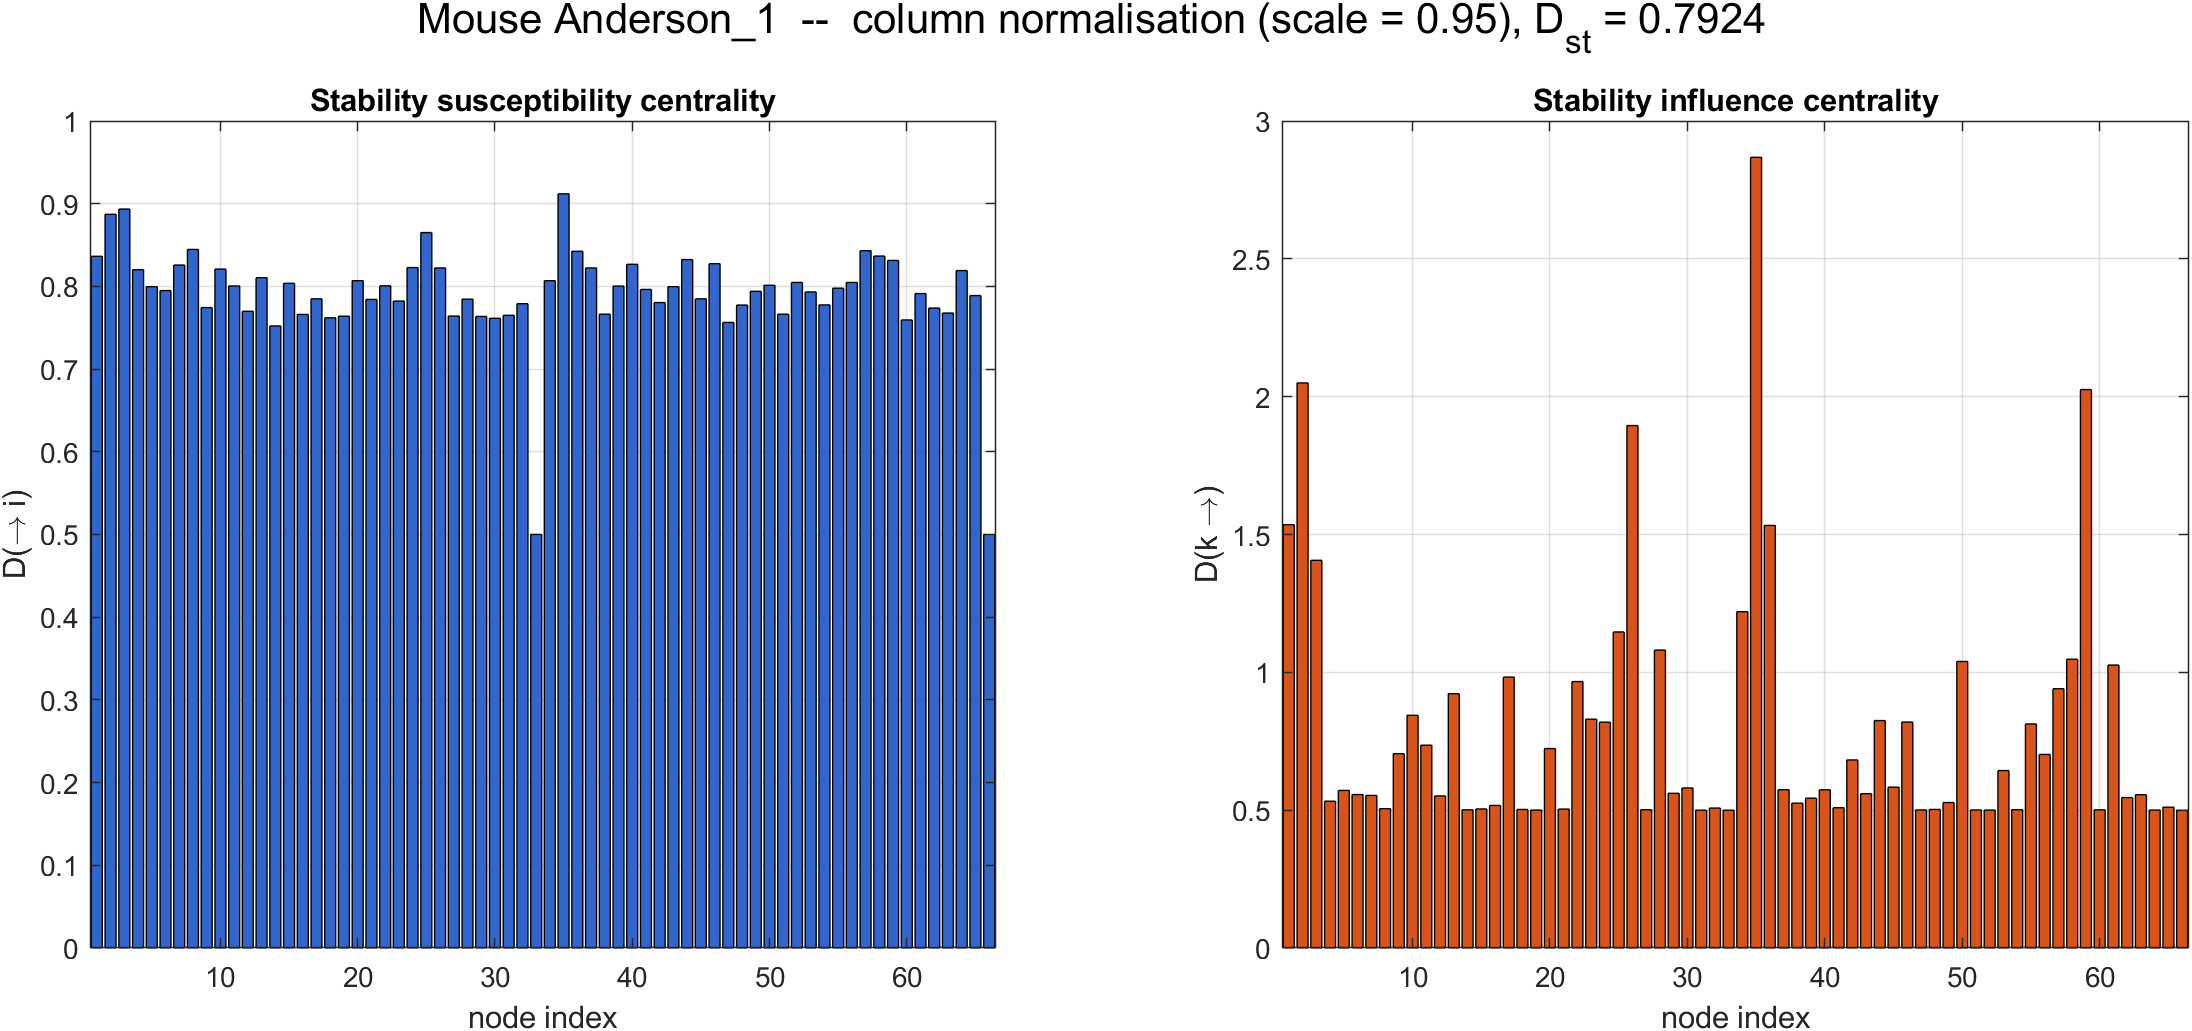
\includegraphics[width=\linewidth]{appendix/stabilityCentralities_Anderson_1_column_figure.png}
\caption{\textsc{Anderson\_1}}
\end{subfigure}\hfill
\begin{subfigure}{0.32\textwidth}\centering
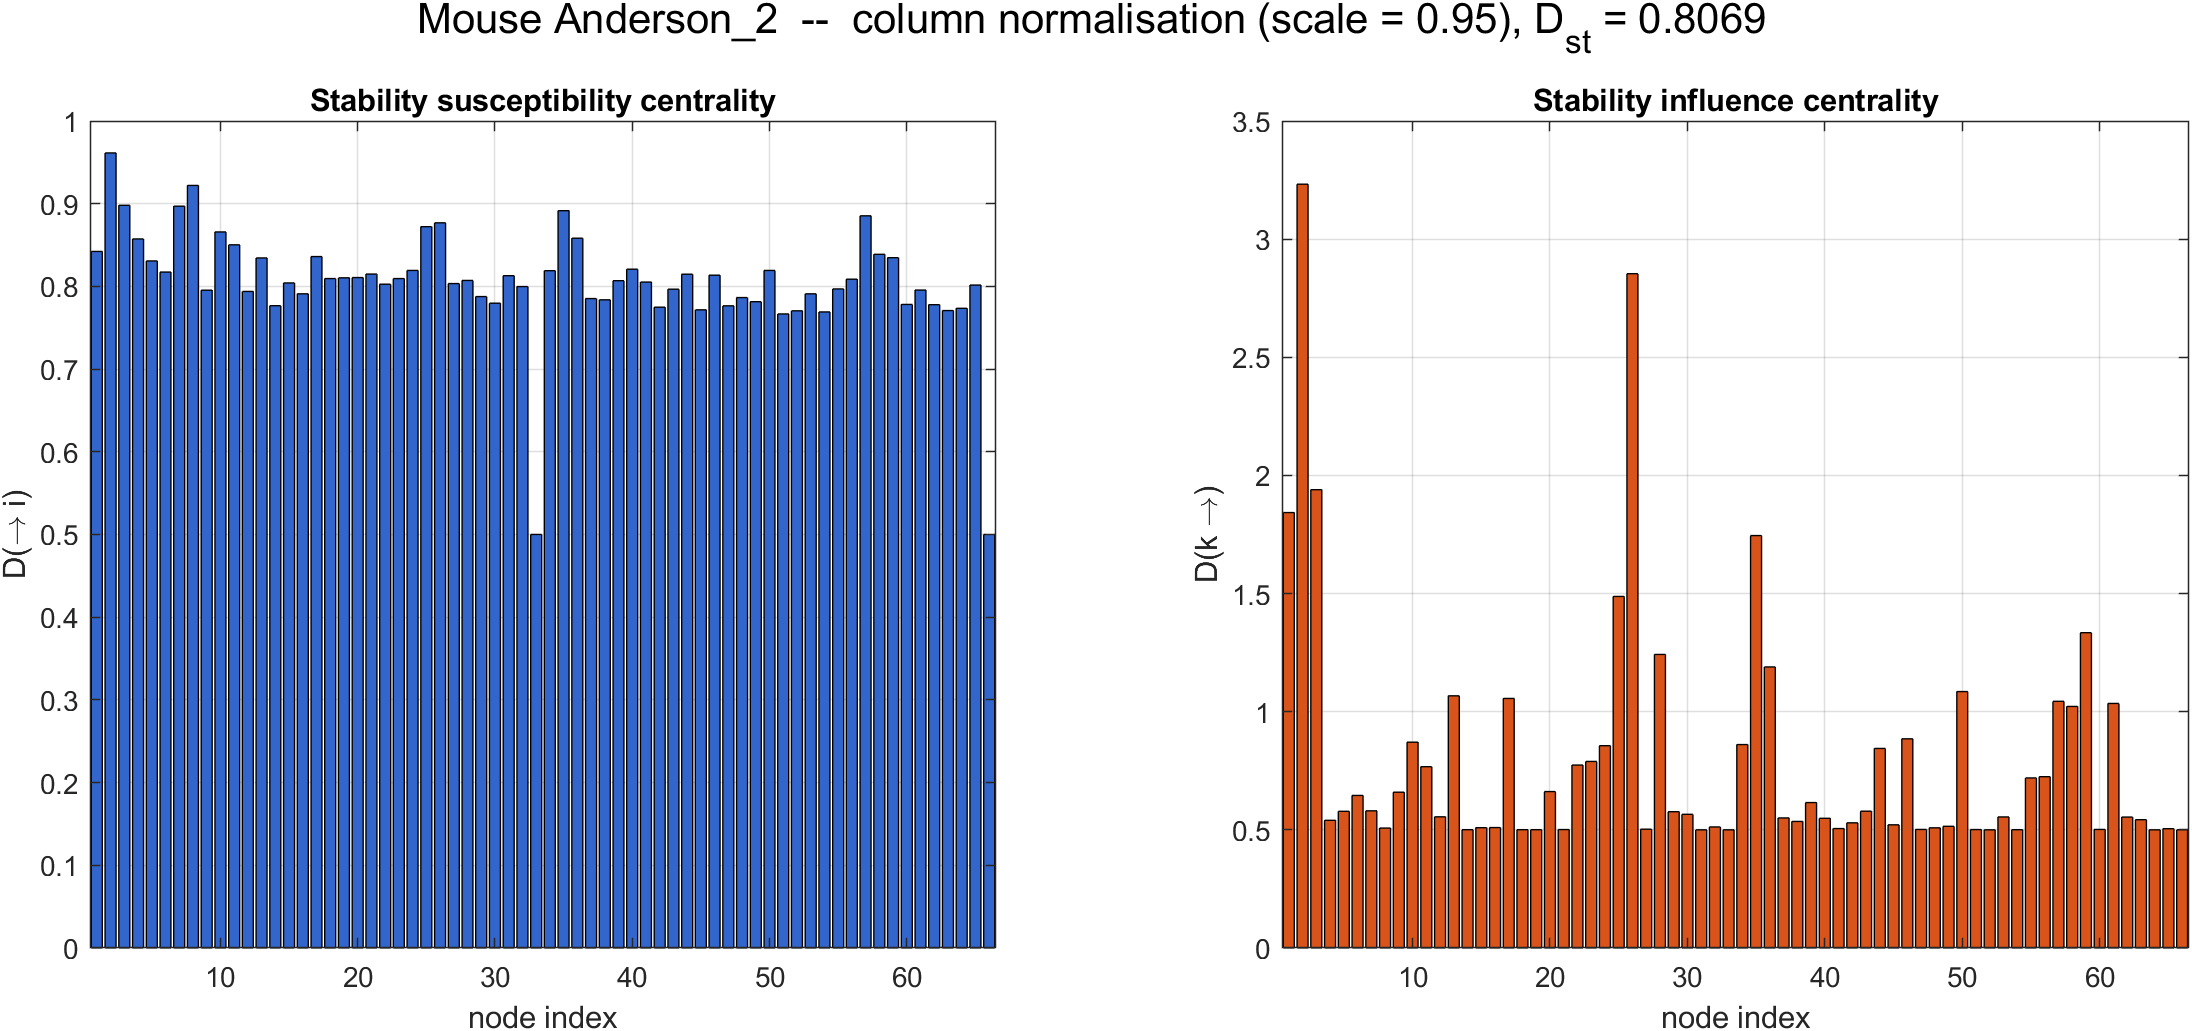
\includegraphics[width=\linewidth]{appendix/stabilityCentralities_Anderson_2_column_figure.png}
\caption{\textsc{Anderson\_2}}
\end{subfigure}\hfill
\begin{subfigure}{0.32\textwidth}\centering
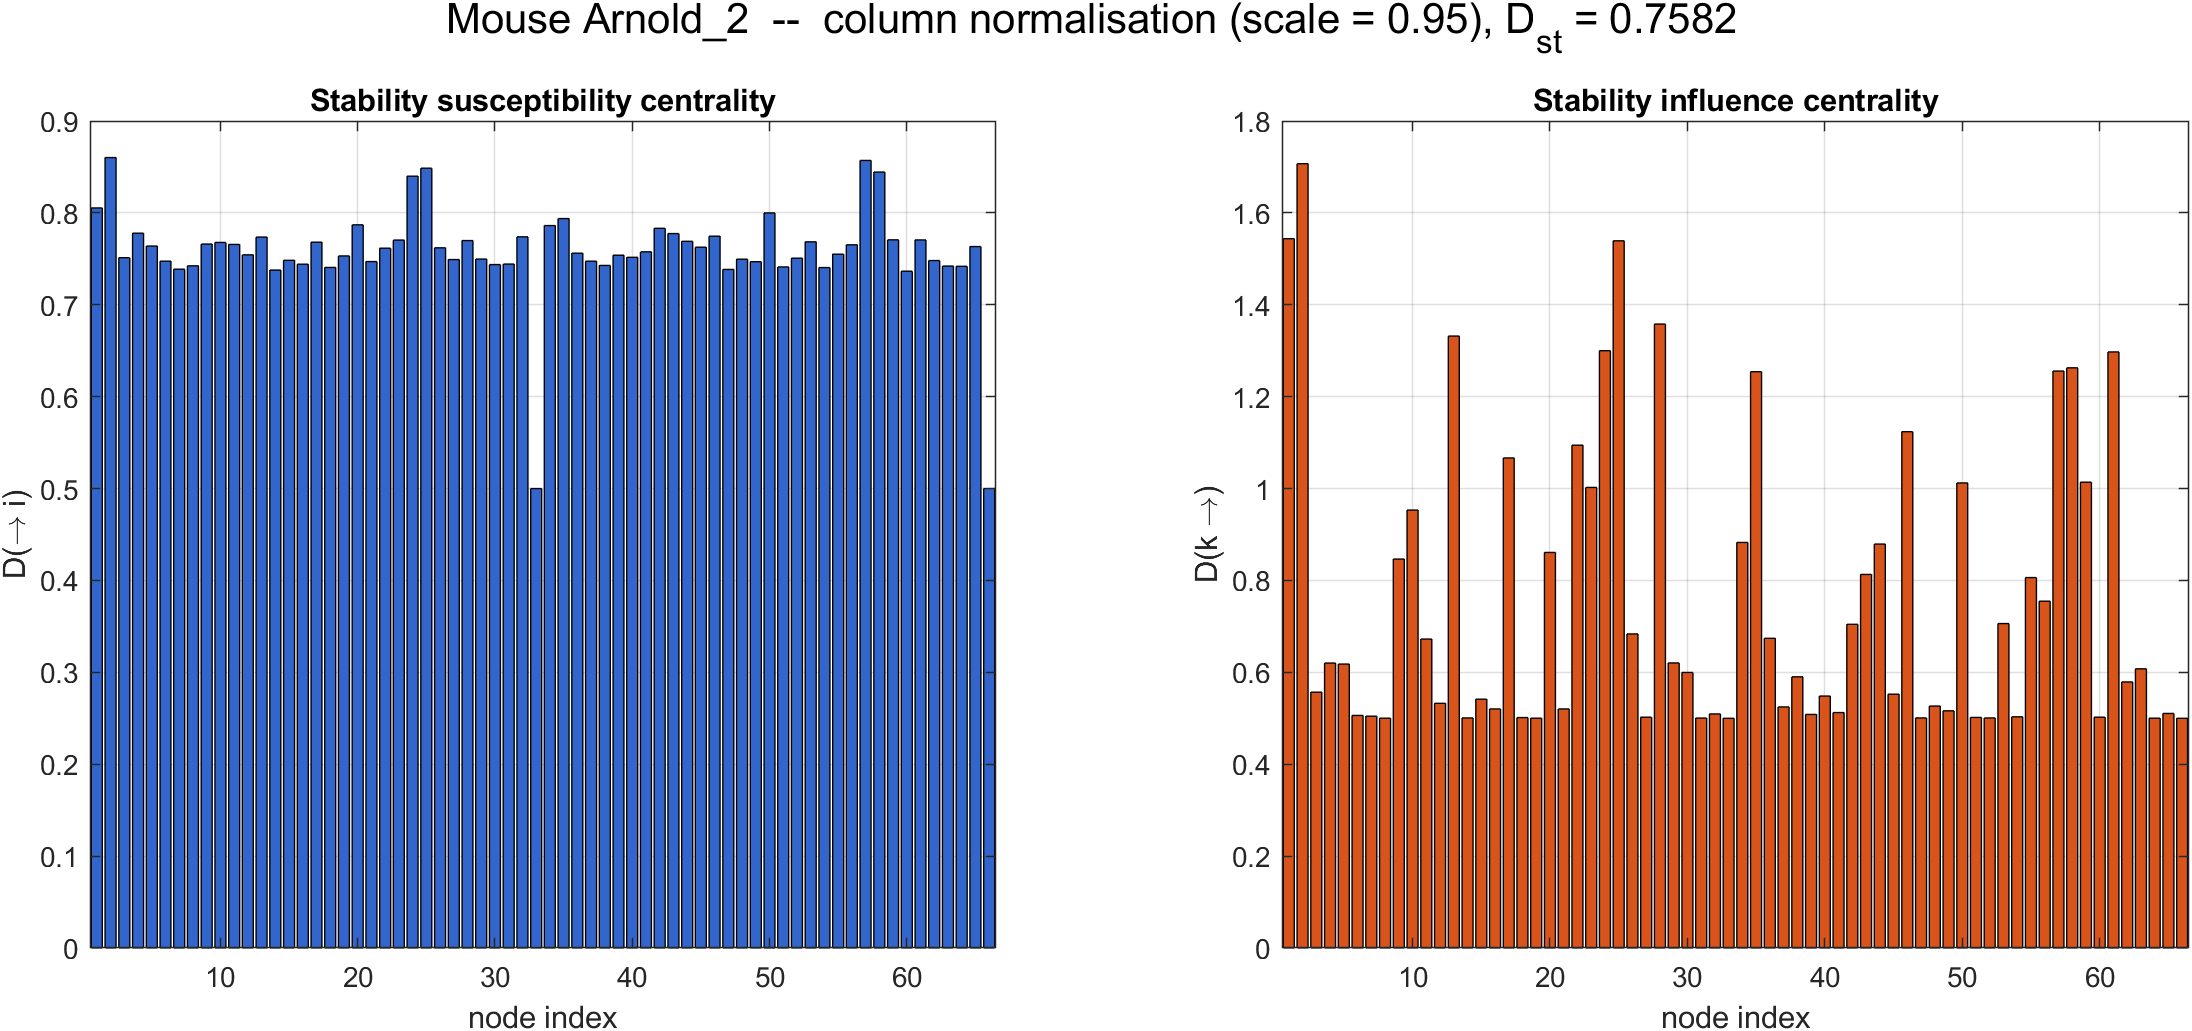
\includegraphics[width=\linewidth]{appendix/stabilityCentralities_Arnold_2_column_figure.png}
\caption{\textsc{Arnold\_2}}
\end{subfigure}\hfill
\begin{subfigure}{0.32\textwidth}\centering
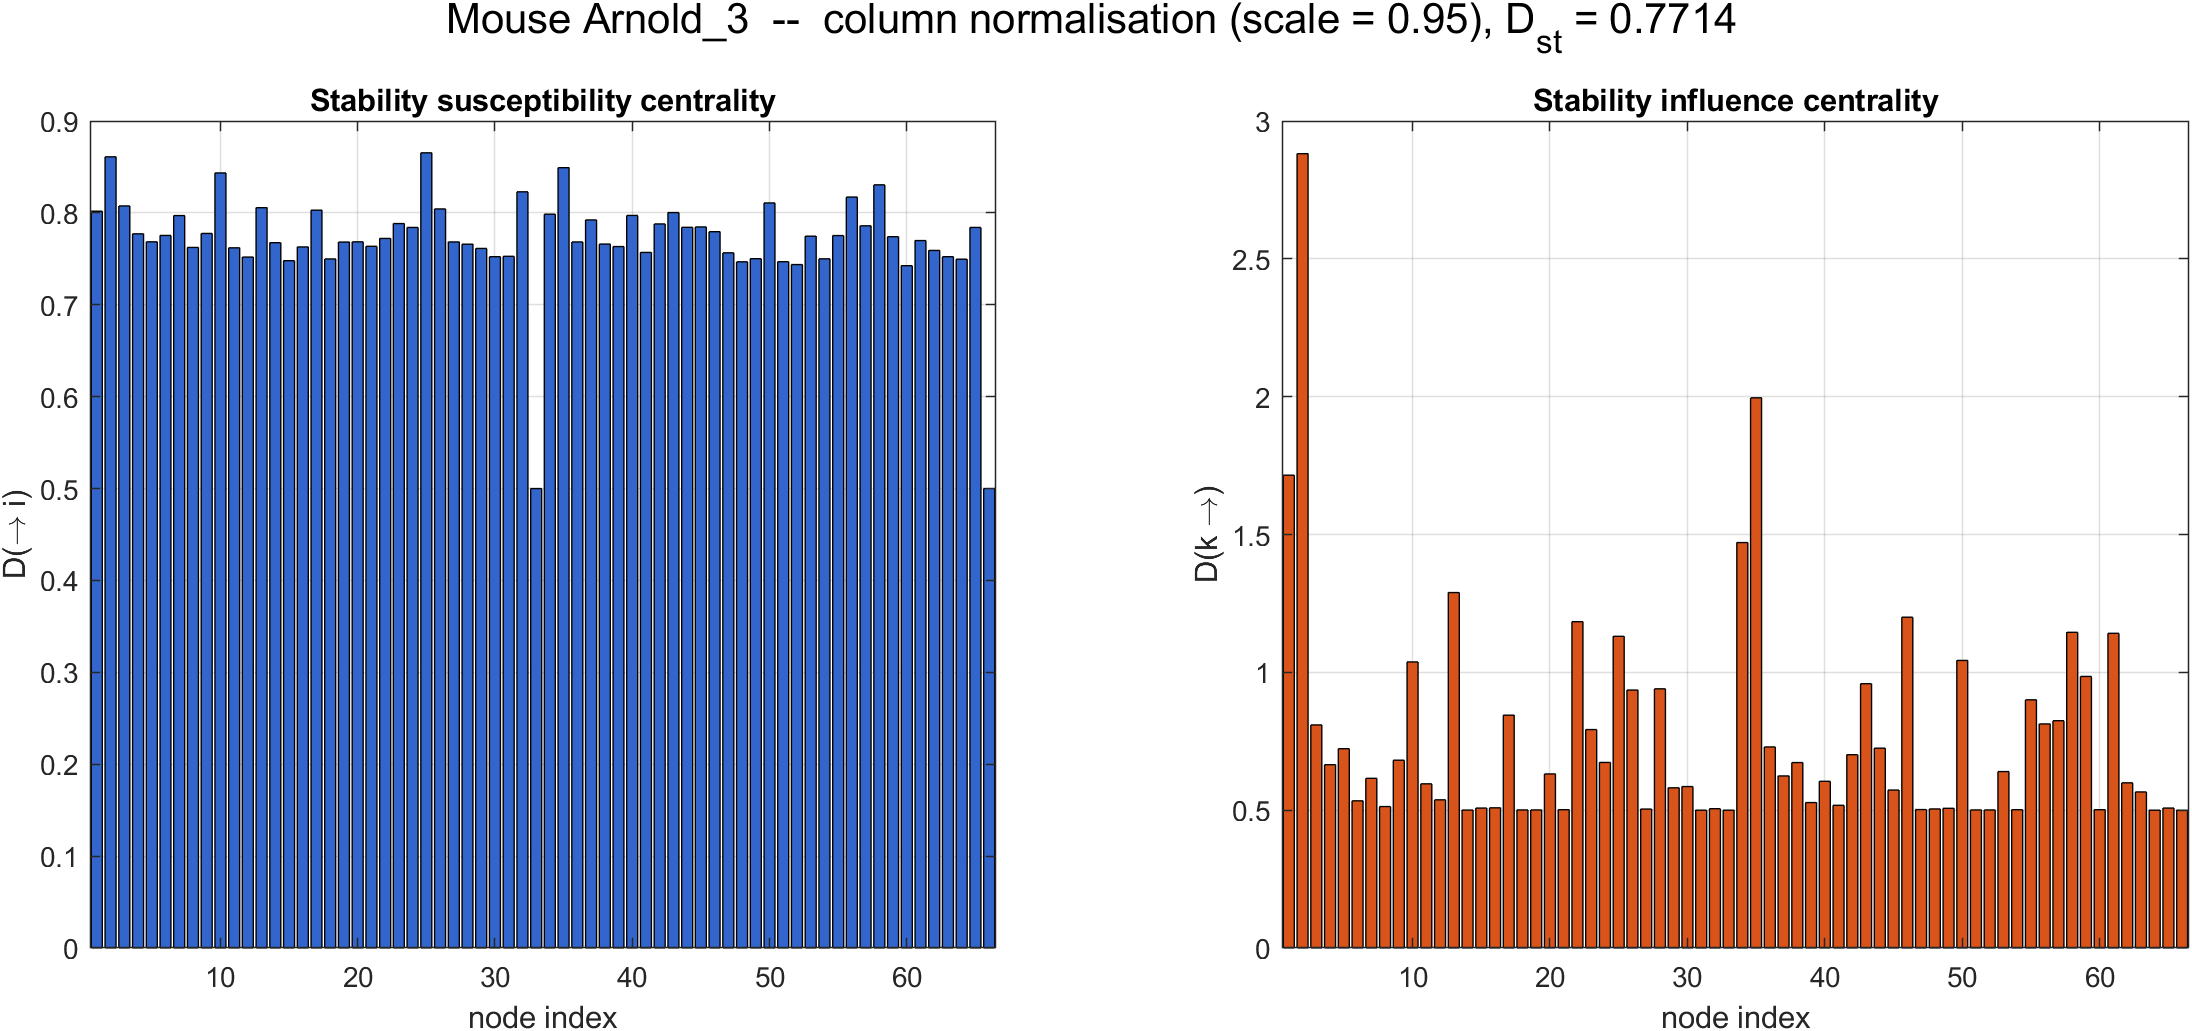
\includegraphics[width=\linewidth]{appendix/stabilityCentralities_Arnold_3_column_figure.png}
\caption{\textsc{Arnold\_3}}
\end{subfigure}\hfill
\begin{subfigure}{0.32\textwidth}\centering
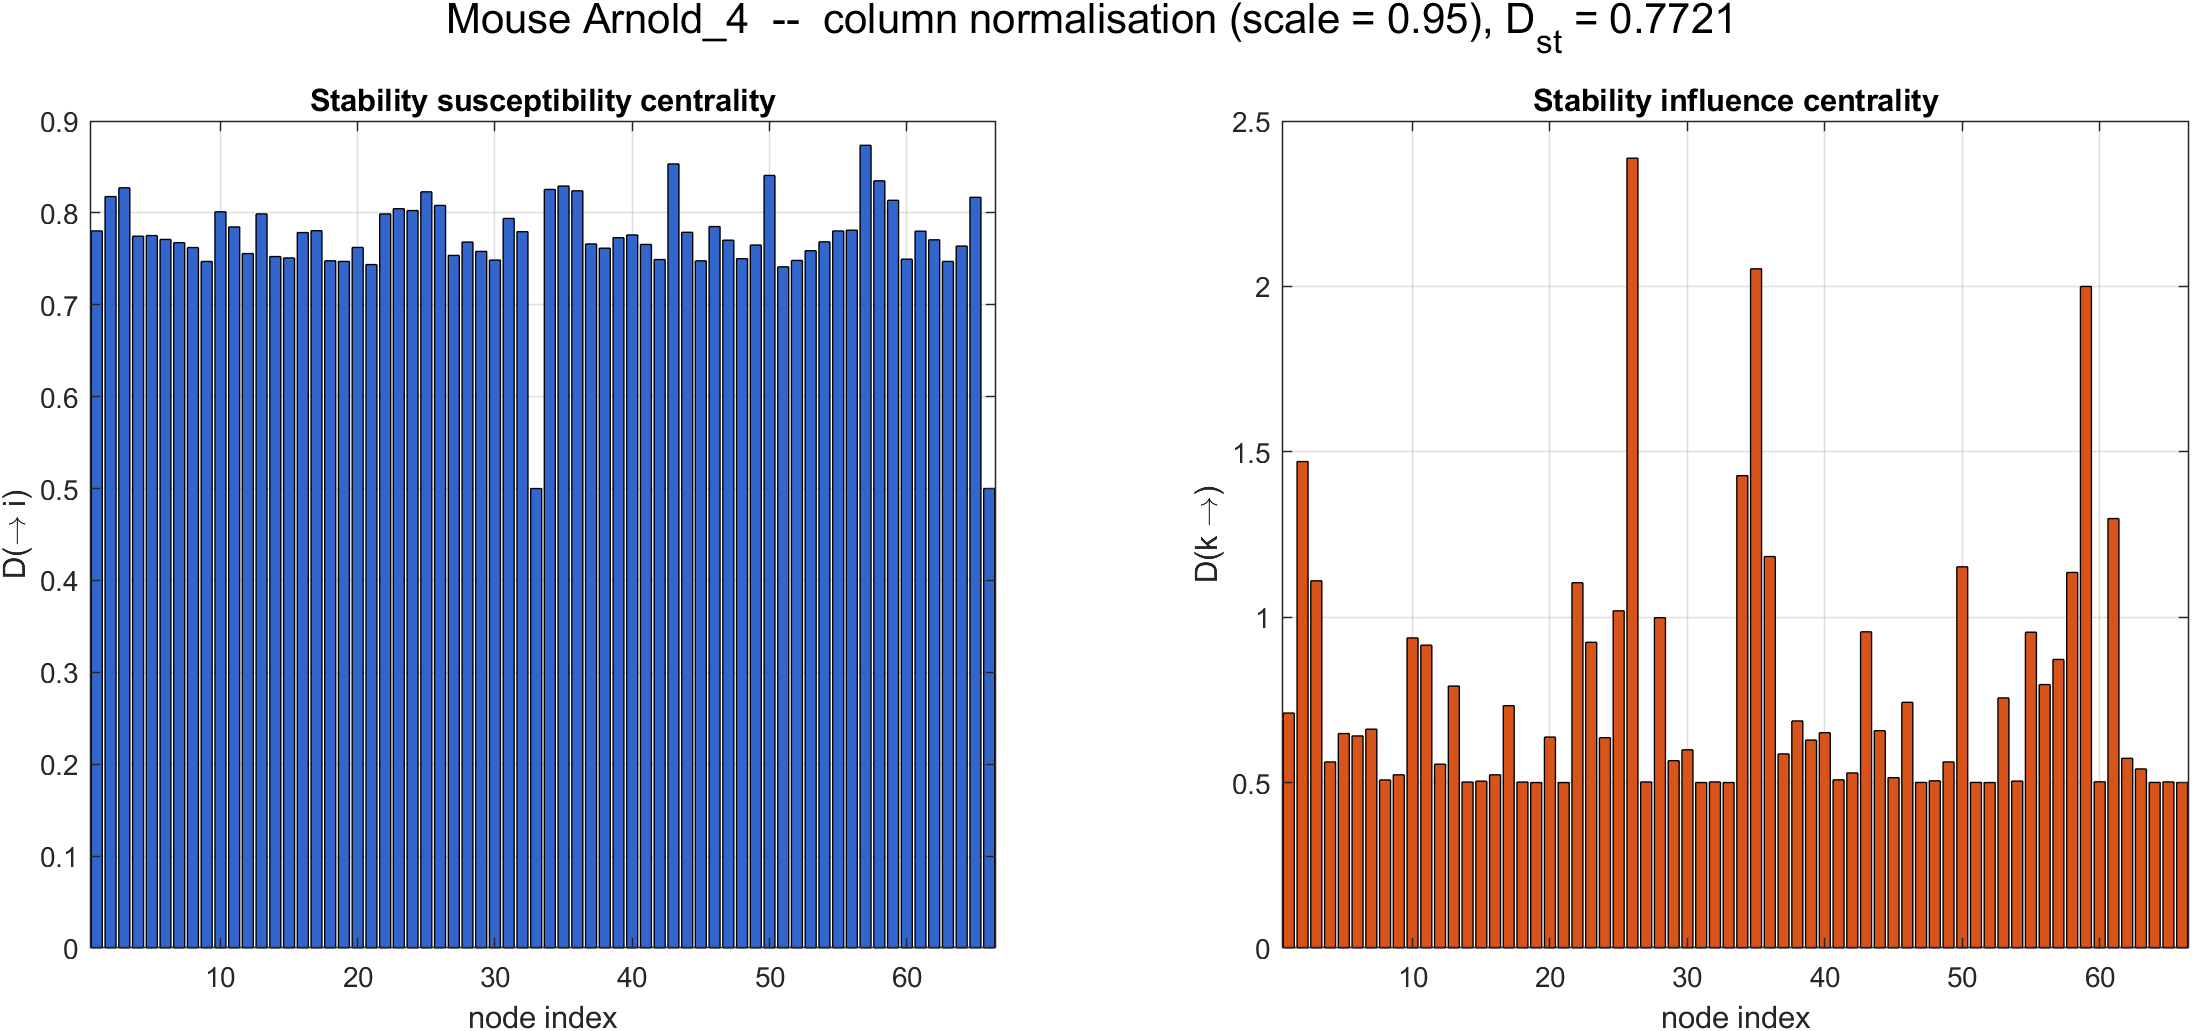
\includegraphics[width=\linewidth]{appendix/stabilityCentralities_Arnold_4_column_figure.png}
\caption{\textsc{Arnold\_4}}
\end{subfigure}\hfill
\begin{subfigure}{0.32\textwidth}\centering
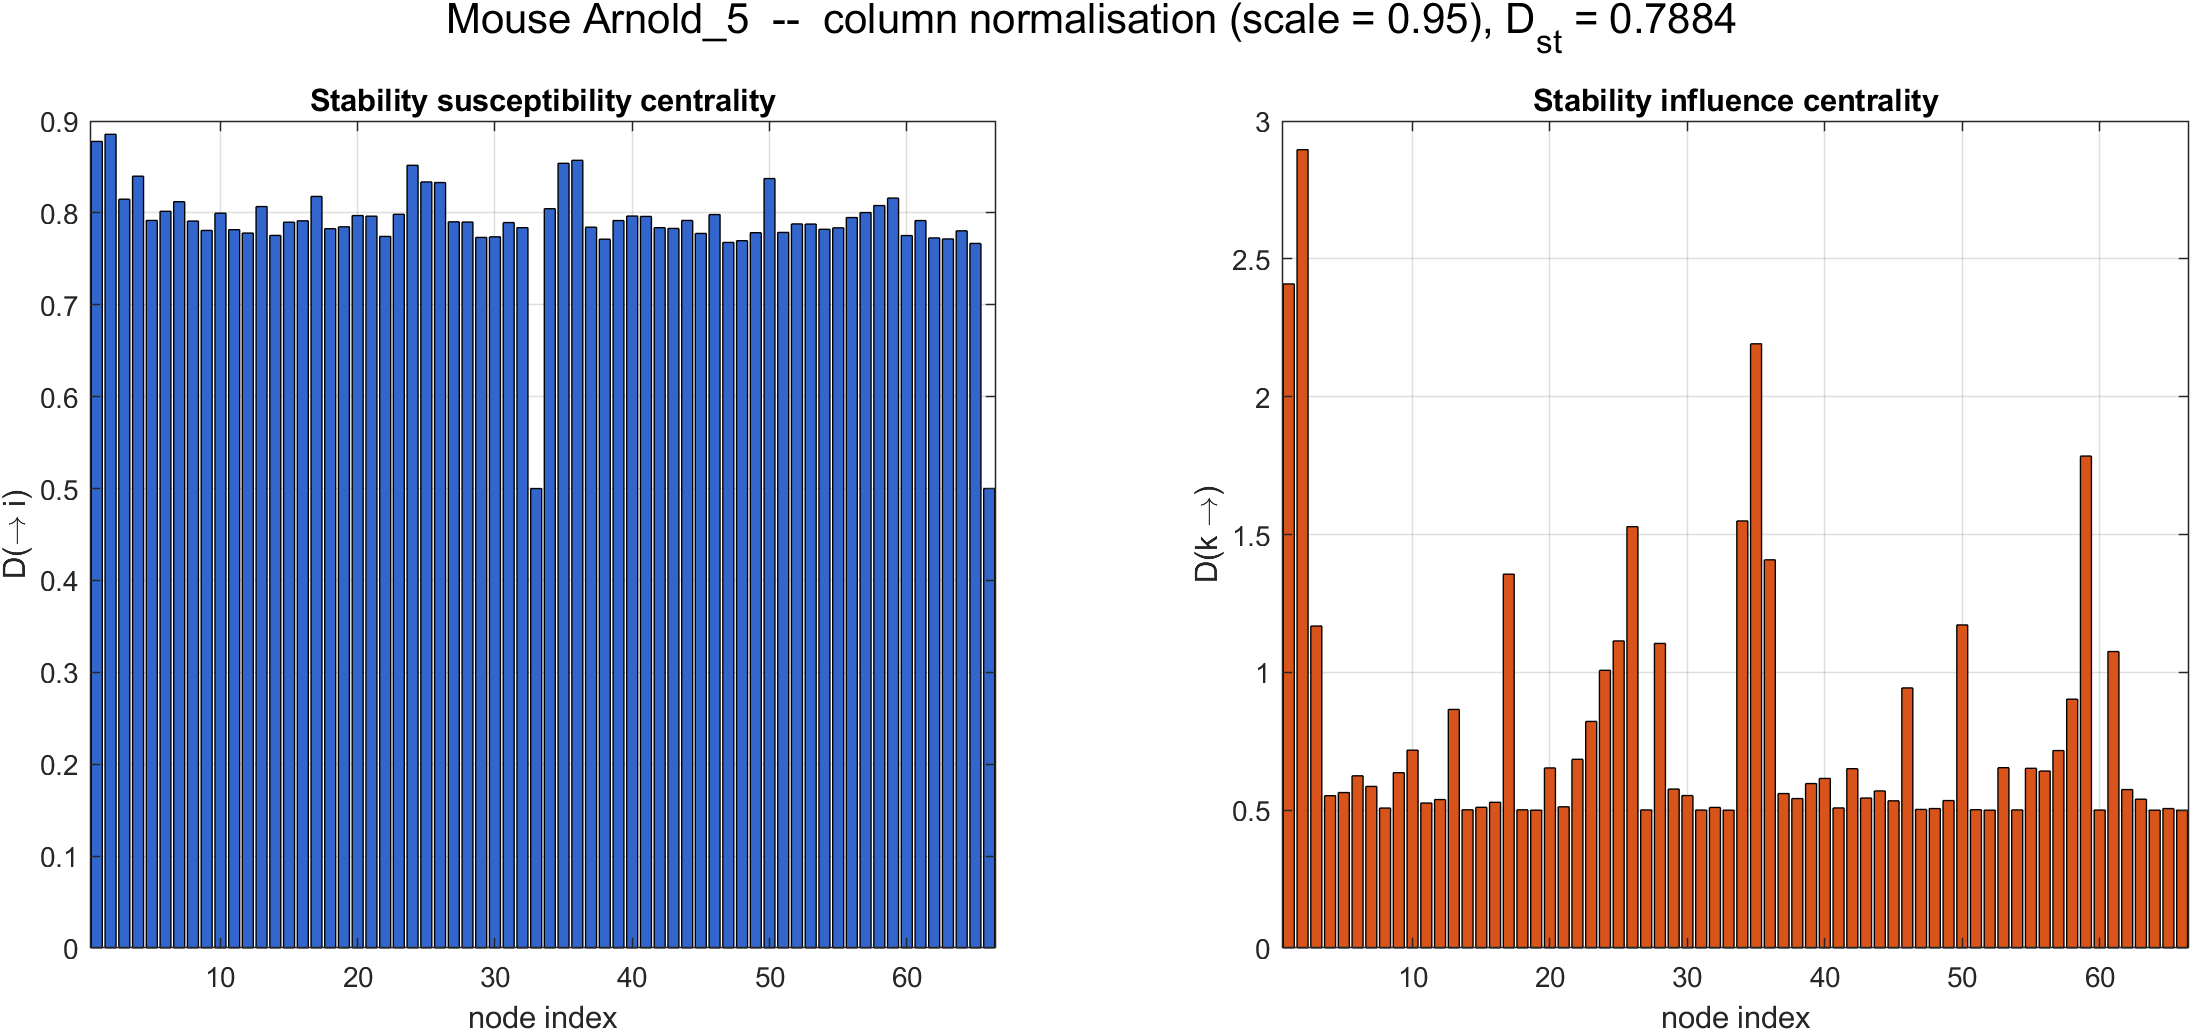
\includegraphics[width=\linewidth]{appendix/stabilityCentralities_Arnold_5_column_figure.png}
\caption{\textsc{Arnold\_5}}
\end{subfigure}\hfill
\caption{Per-region susceptibility $\Dto$ and influence $\Dfrom$ for all six mice, \texttt{column} scheme.}
\end{figure}
\begin{figure}[H]\centering
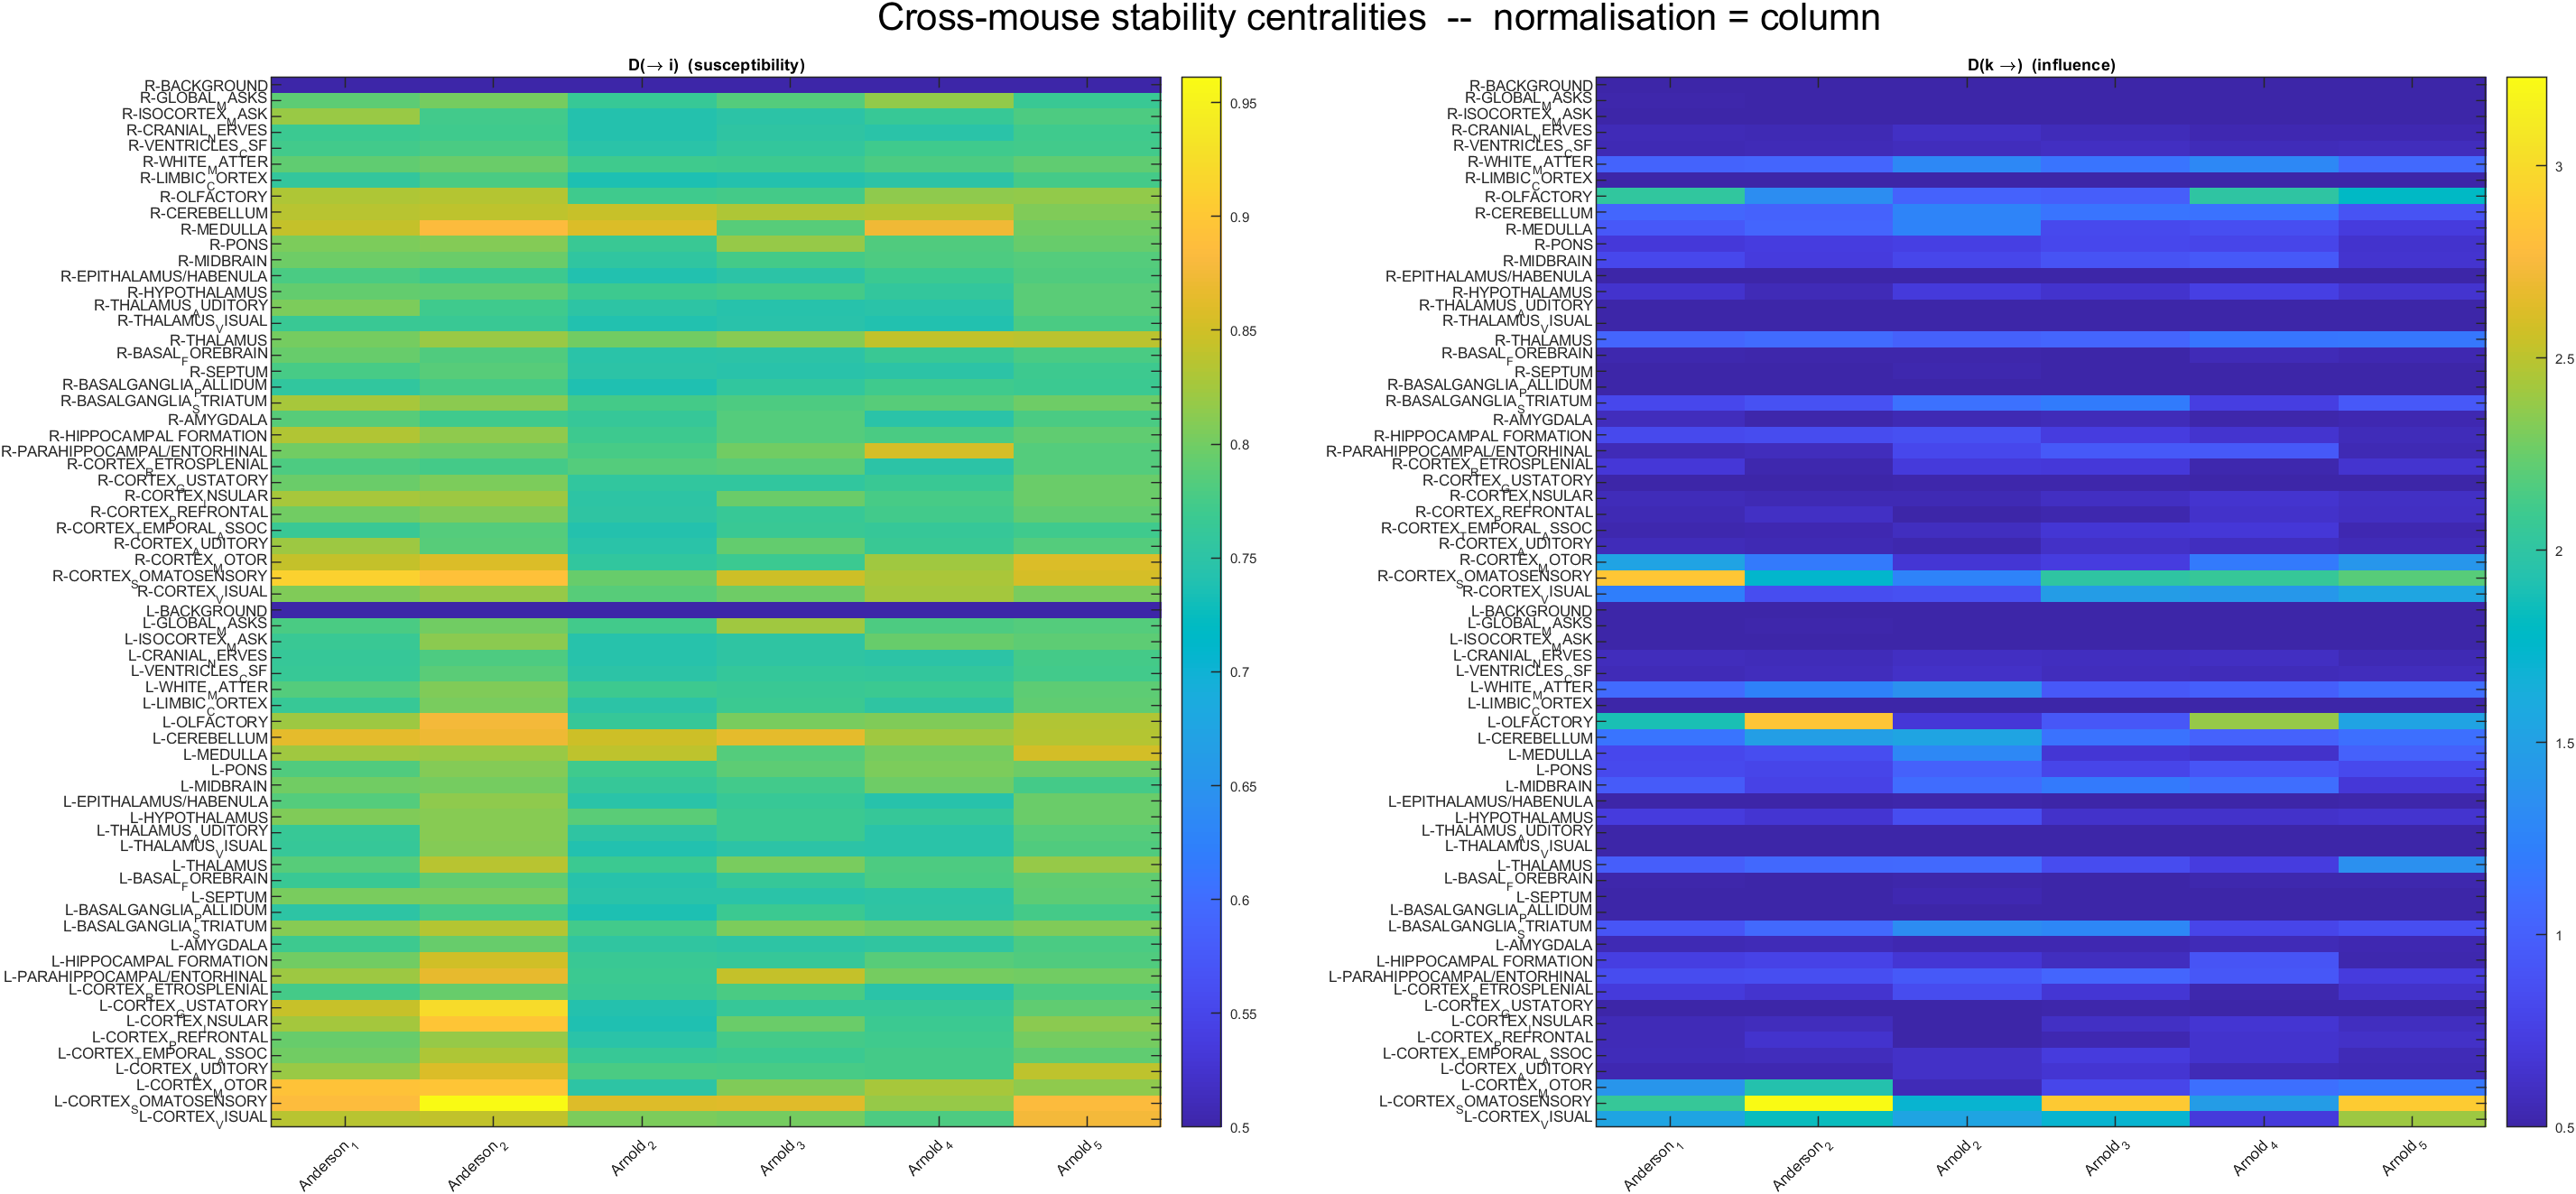
\includegraphics[width=0.8\textwidth]{appendix/stabilityCentralities_summary_overview_column.png}
\caption{Cohort overview of stability centralities, \texttt{column} scheme.}
\end{figure}

\begin{figure}[H]\centering
\begin{subfigure}{0.32\textwidth}\centering
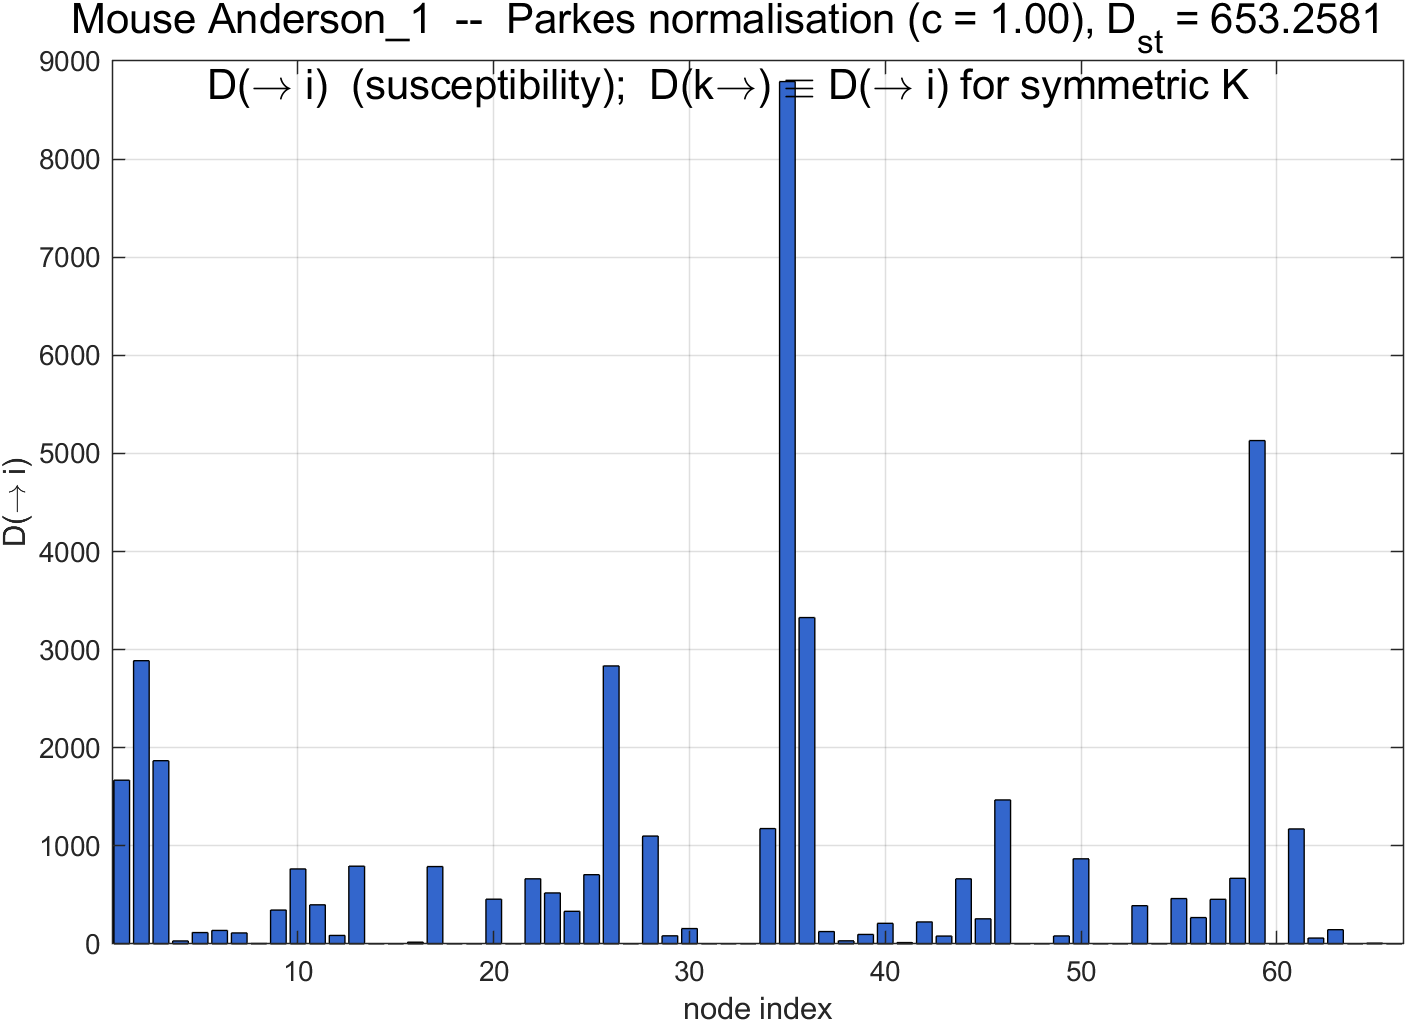
\includegraphics[width=\linewidth]{appendix/stabilityCentralities_Anderson_1_parkes_figure.png}
\caption{\textsc{Anderson\_1}}
\end{subfigure}\hfill
\begin{subfigure}{0.32\textwidth}\centering
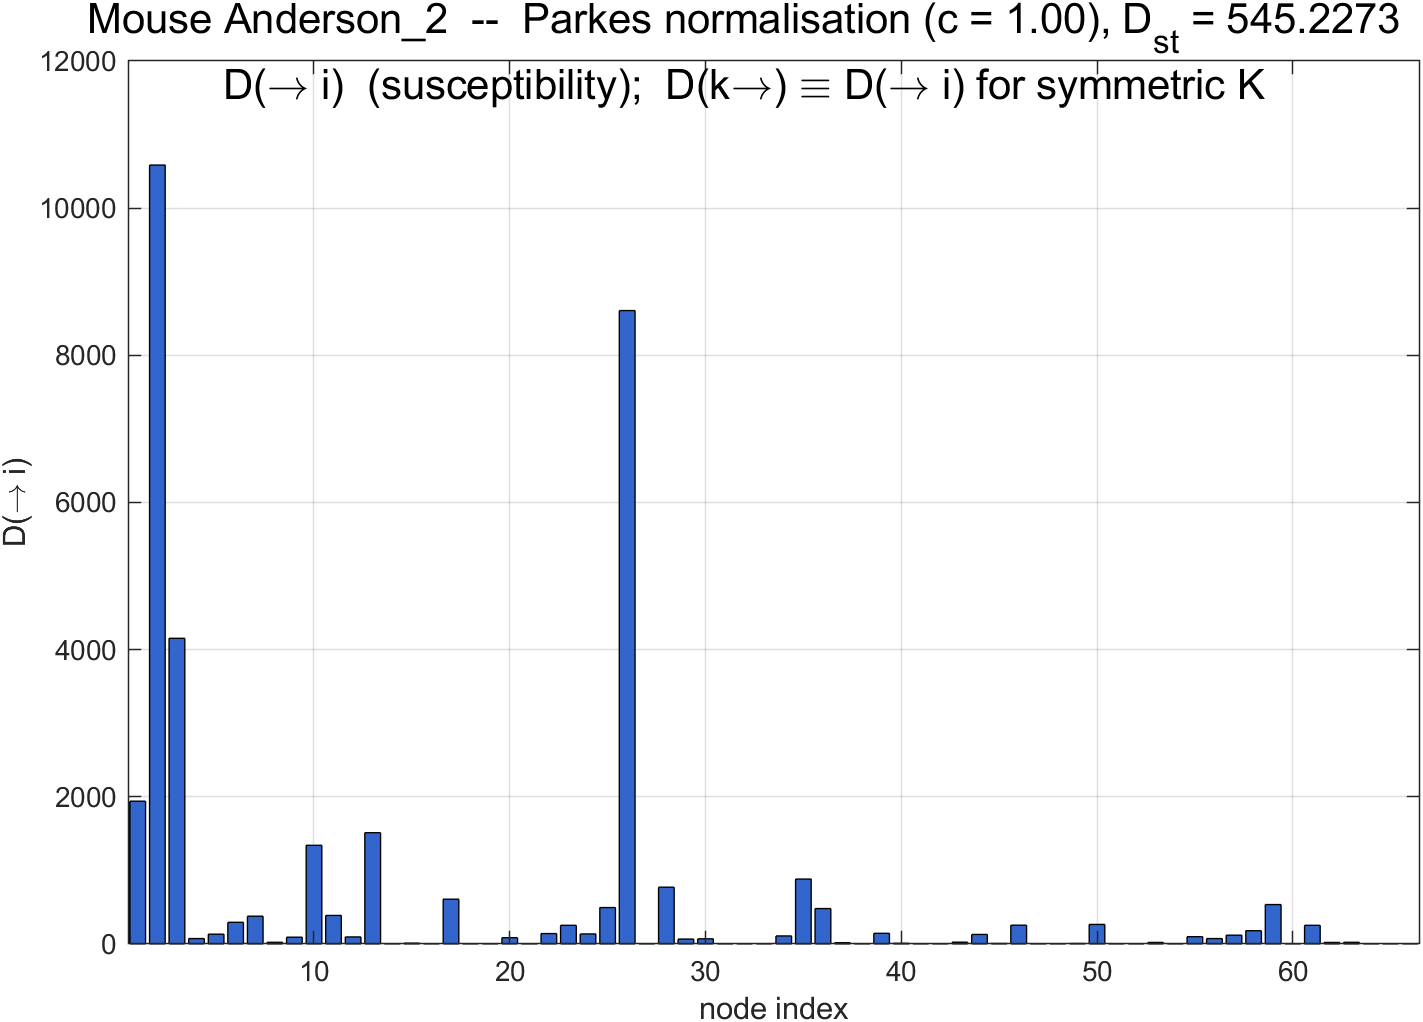
\includegraphics[width=\linewidth]{appendix/stabilityCentralities_Anderson_2_parkes_figure.png}
\caption{\textsc{Anderson\_2}}
\end{subfigure}\hfill
\begin{subfigure}{0.32\textwidth}\centering
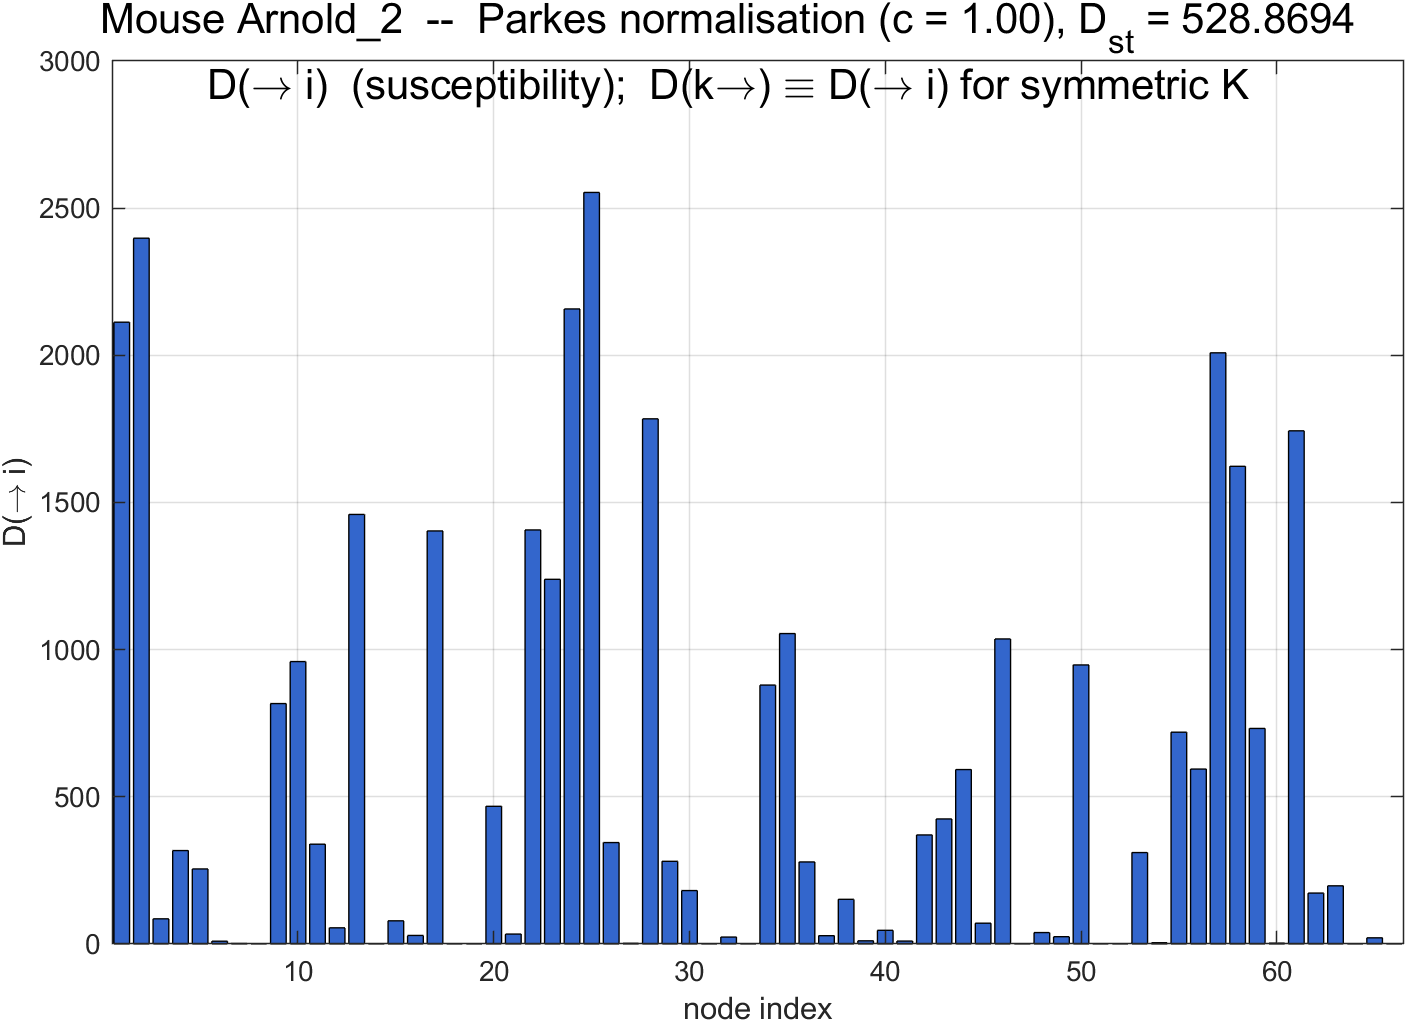
\includegraphics[width=\linewidth]{appendix/stabilityCentralities_Arnold_2_parkes_figure.png}
\caption{\textsc{Arnold\_2}}
\end{subfigure}\hfill
\begin{subfigure}{0.32\textwidth}\centering
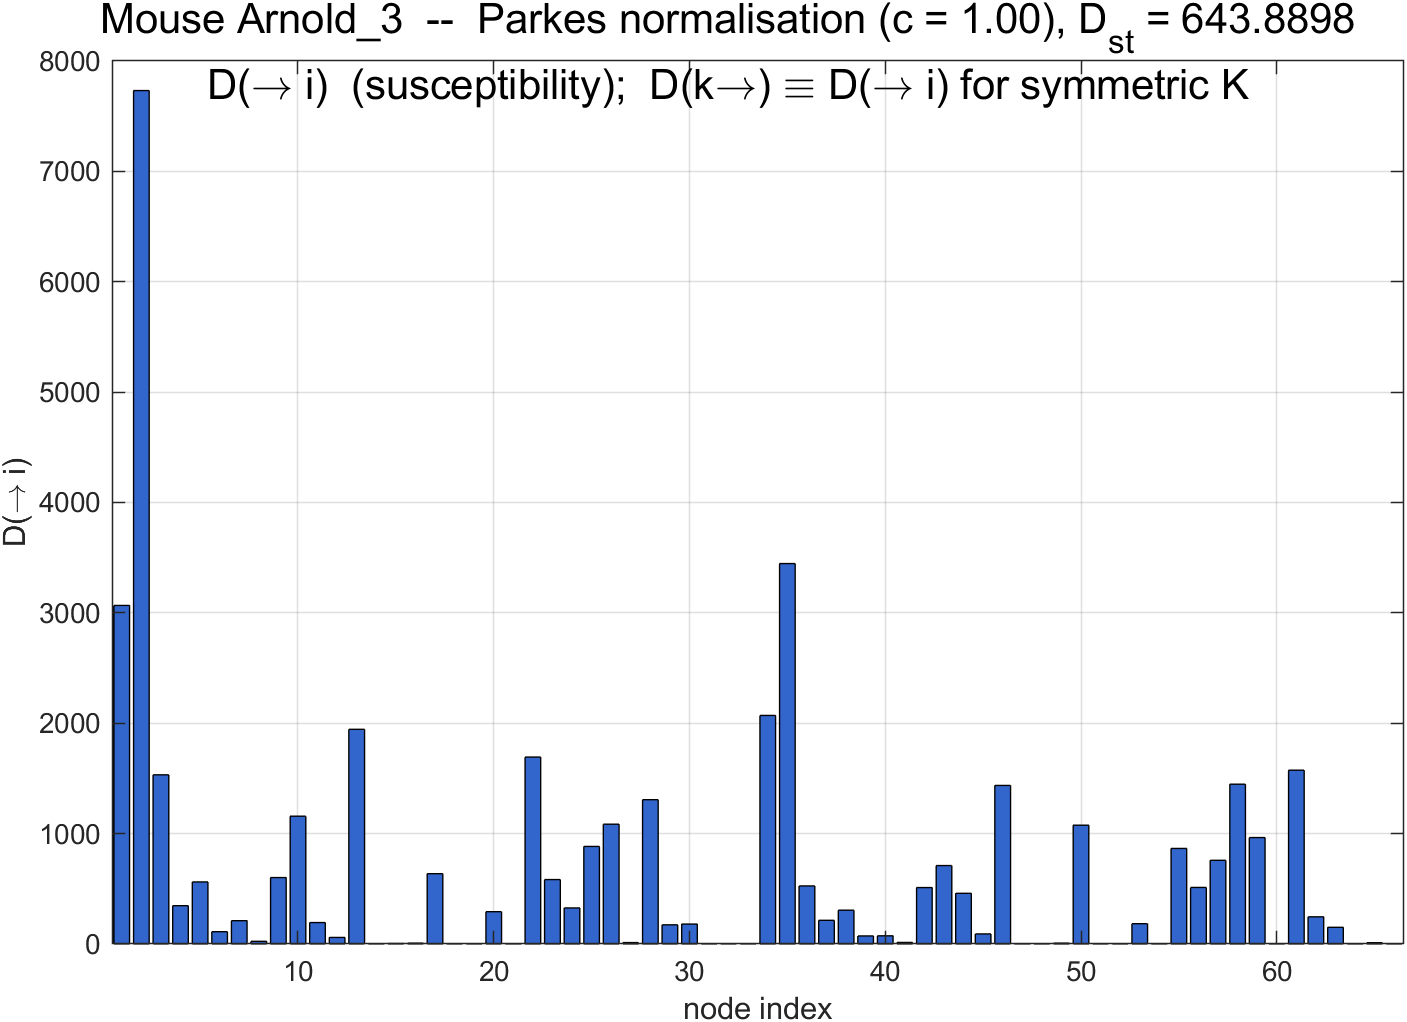
\includegraphics[width=\linewidth]{appendix/stabilityCentralities_Arnold_3_parkes_figure.png}
\caption{\textsc{Arnold\_3}}
\end{subfigure}\hfill
\begin{subfigure}{0.32\textwidth}\centering
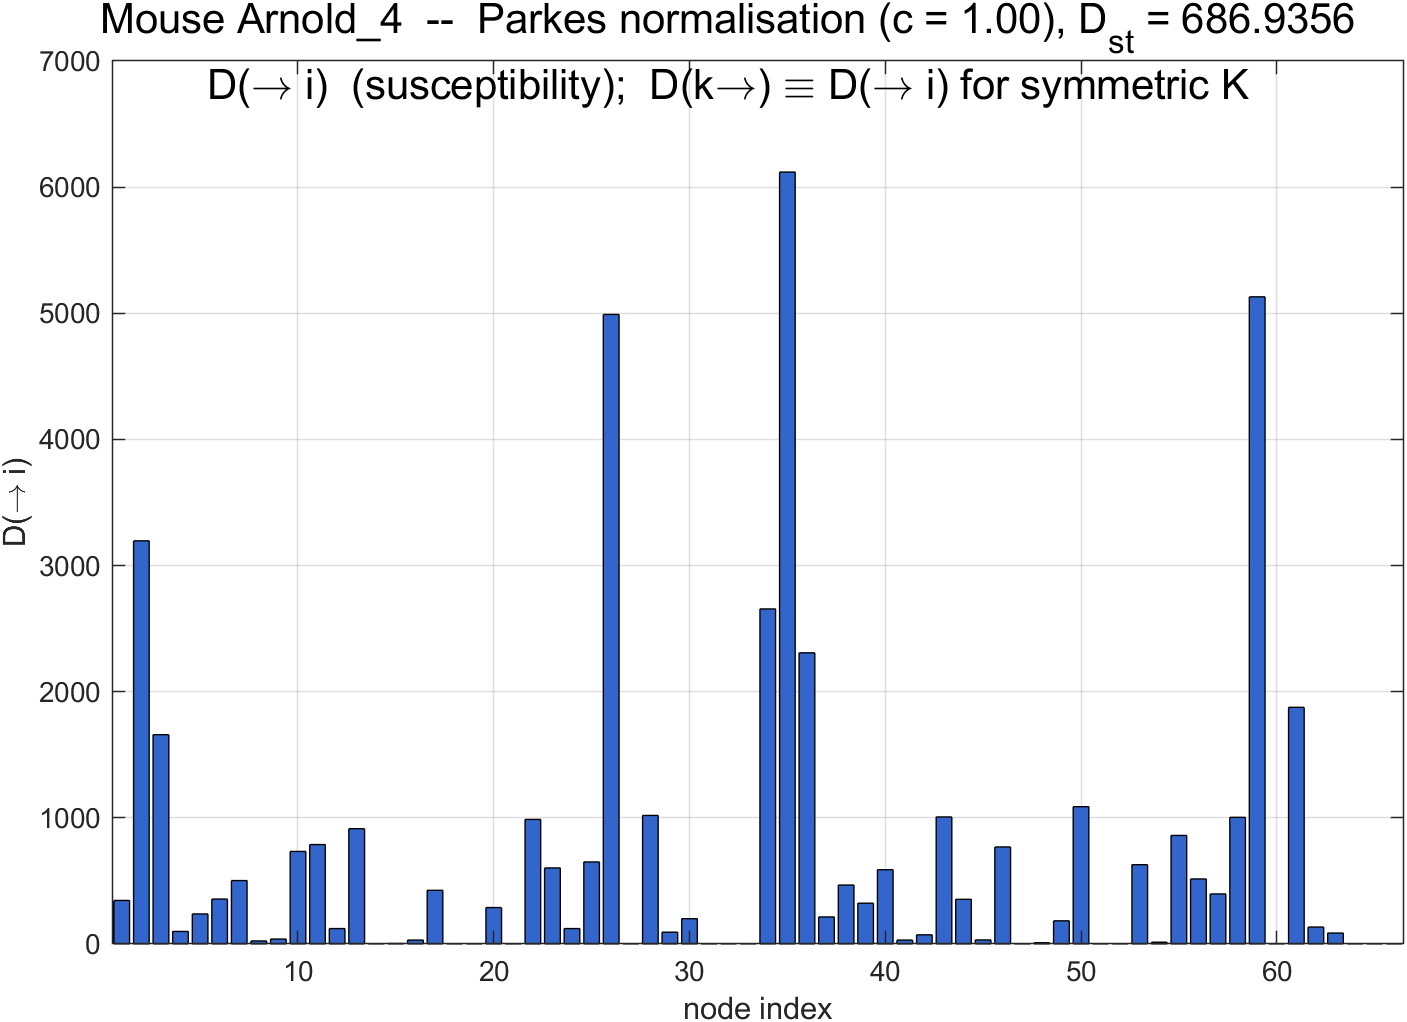
\includegraphics[width=\linewidth]{appendix/stabilityCentralities_Arnold_4_parkes_figure.png}
\caption{\textsc{Arnold\_4}}
\end{subfigure}\hfill
\begin{subfigure}{0.32\textwidth}\centering
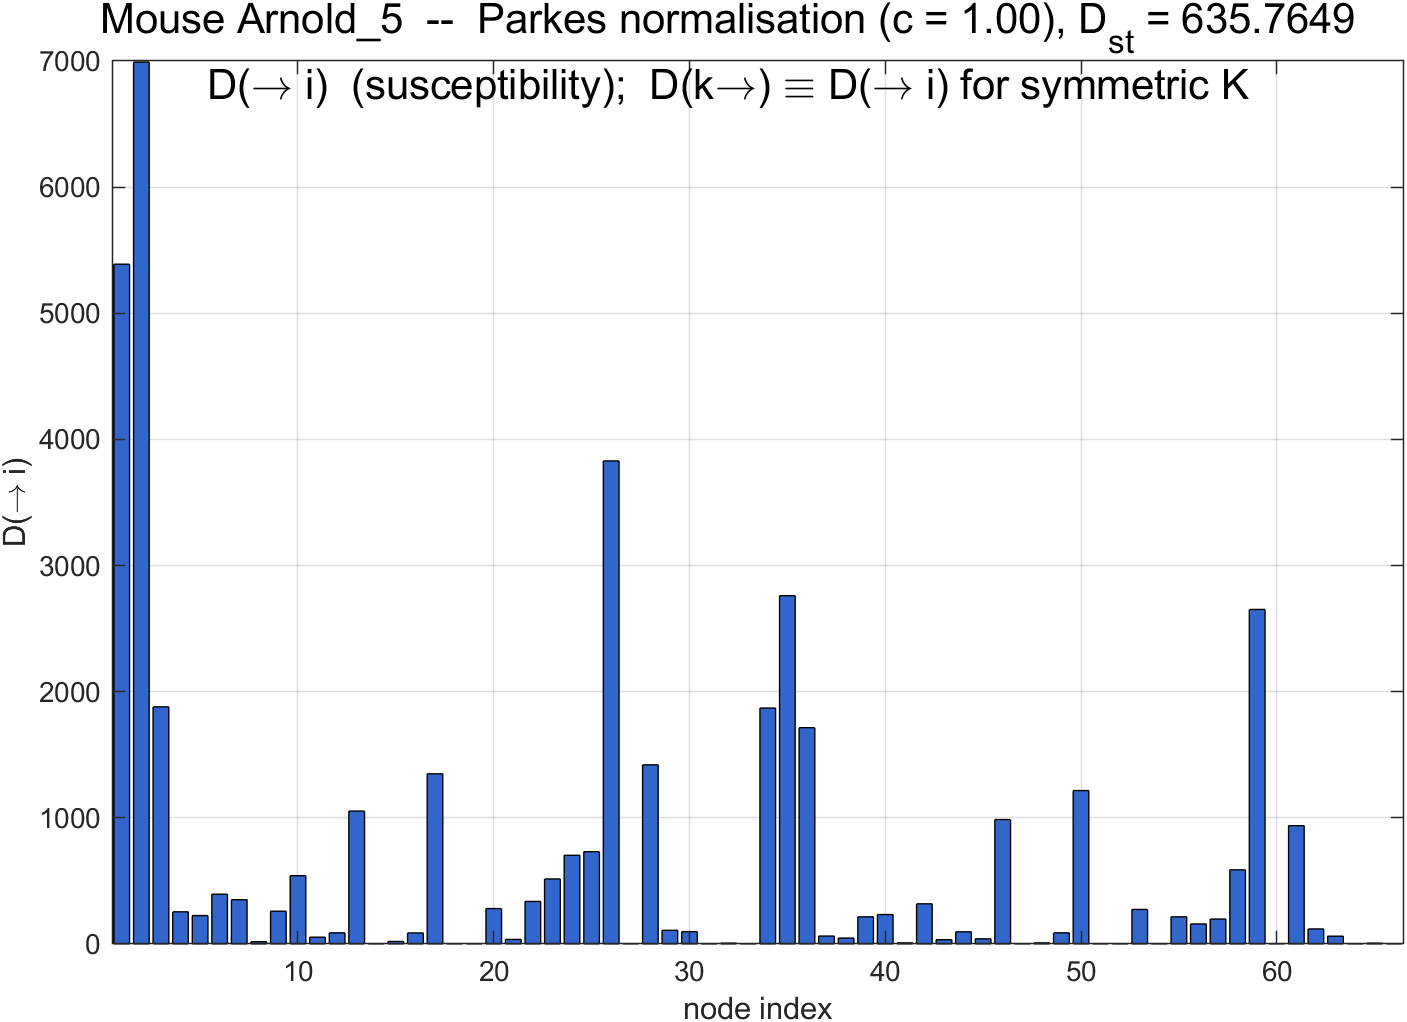
\includegraphics[width=\linewidth]{appendix/stabilityCentralities_Arnold_5_parkes_figure.png}
\caption{\textsc{Arnold\_5}}
\end{subfigure}\hfill
\caption{Per-region susceptibility $\Dto$ and influence $\Dfrom$ for all six mice, \texttt{parkes} scheme.}
\end{figure}
\begin{figure}[H]\centering
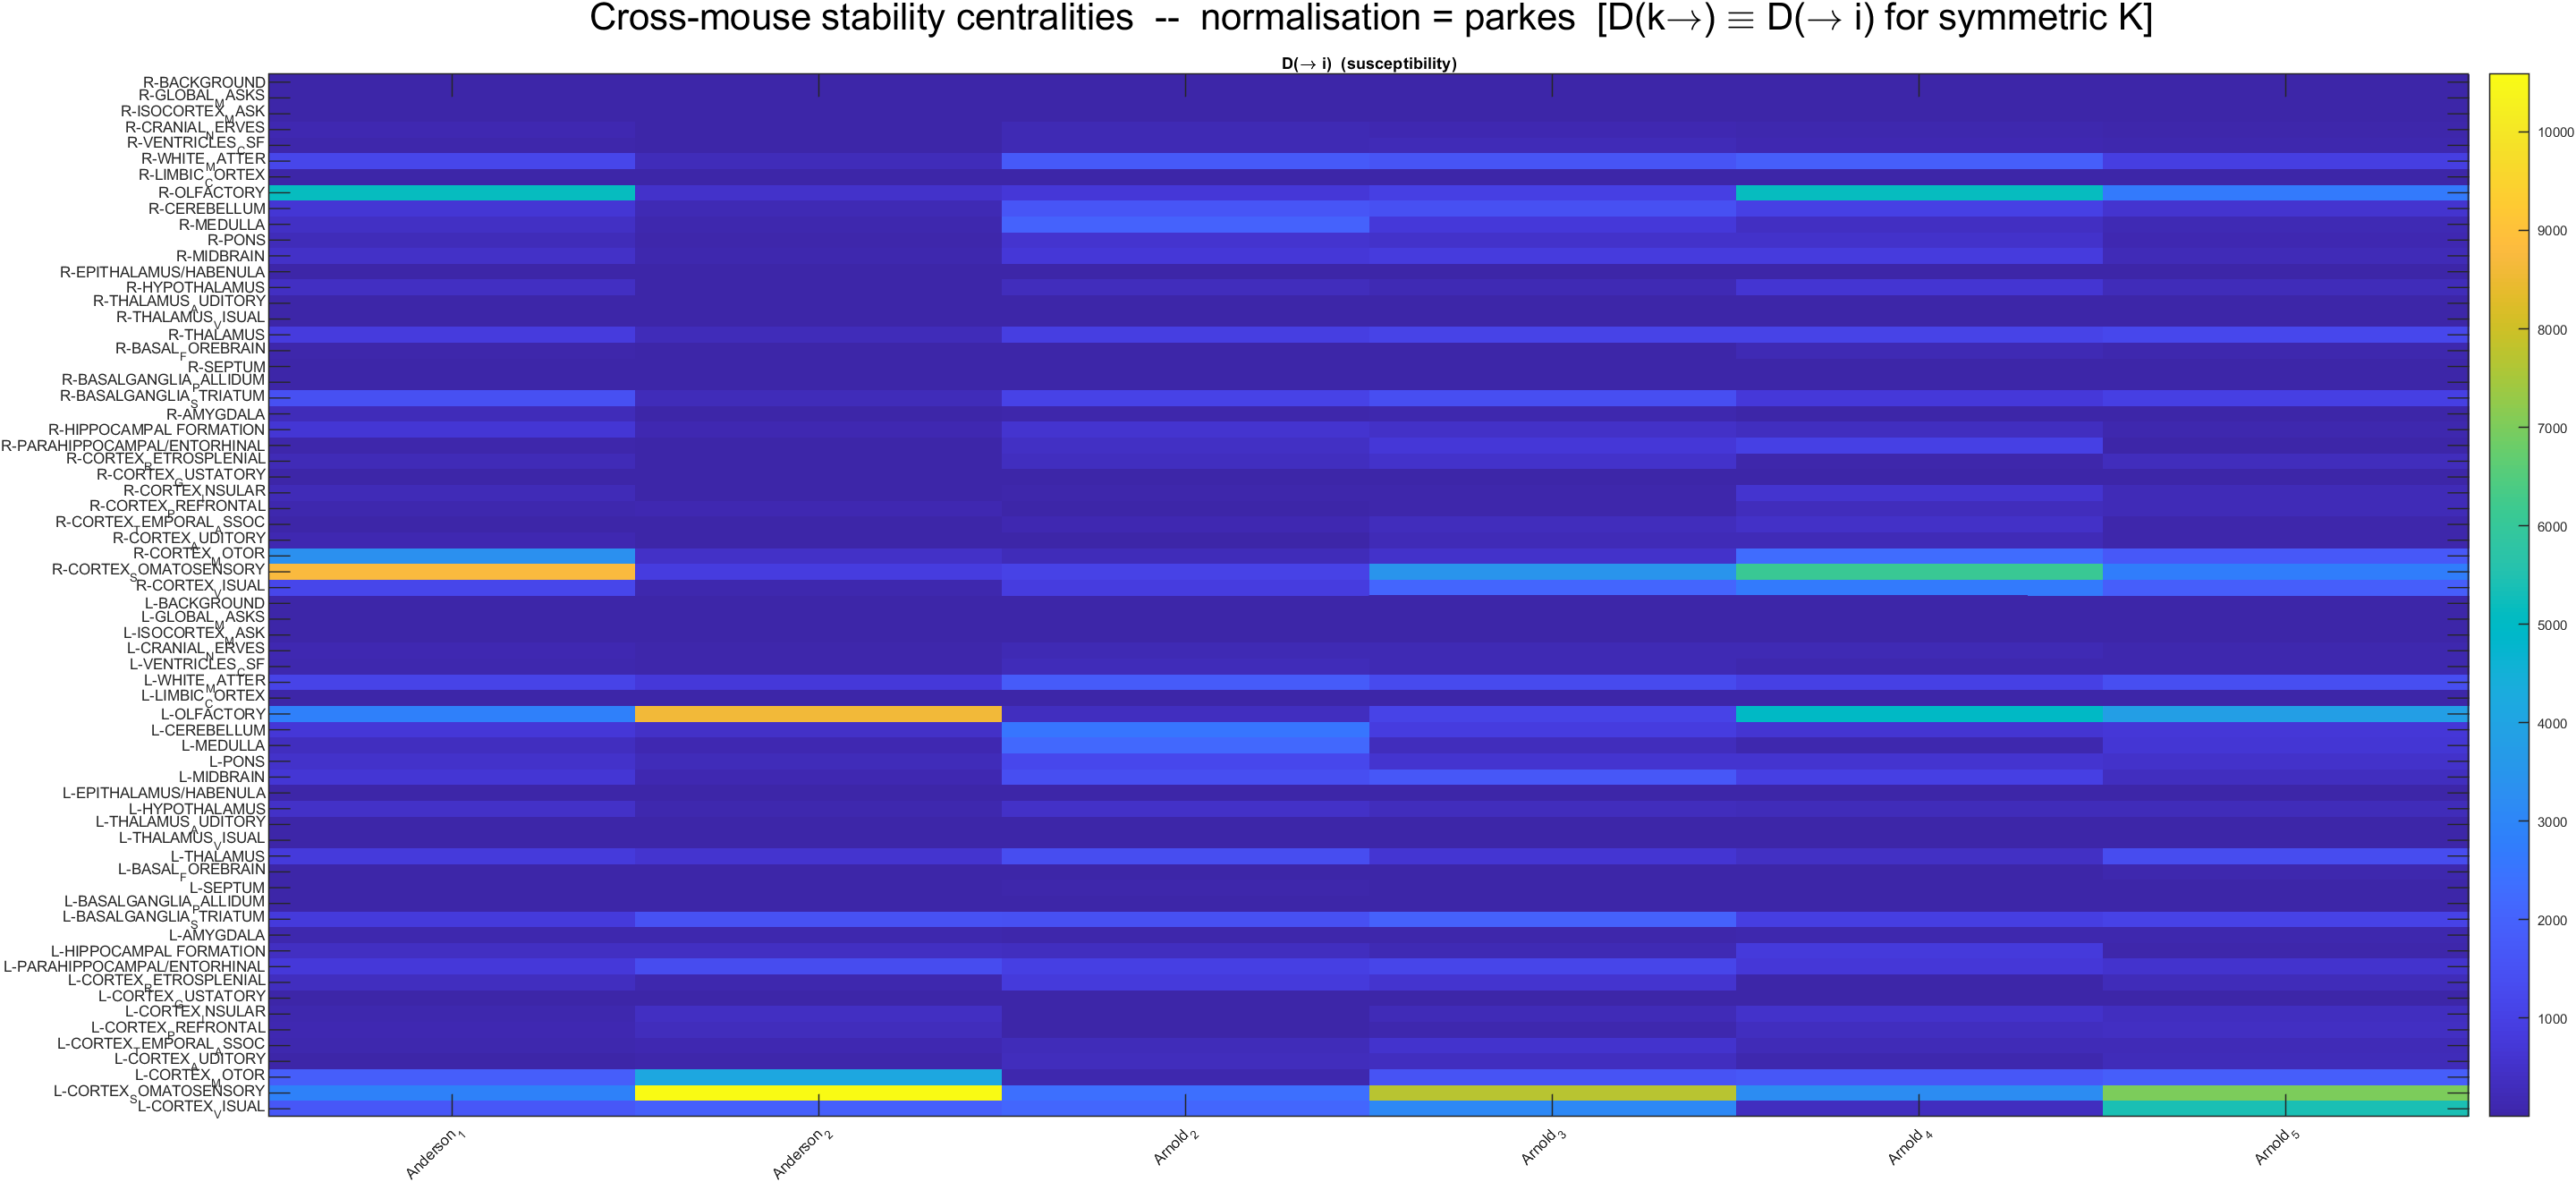
\includegraphics[width=0.8\textwidth]{appendix/stabilityCentralities_summary_overview_parkes.png}
\caption{Cohort overview of stability centralities, \texttt{parkes} scheme.}
\end{figure}

\begin{figure}[H]\centering
\begin{subfigure}{0.32\textwidth}\centering
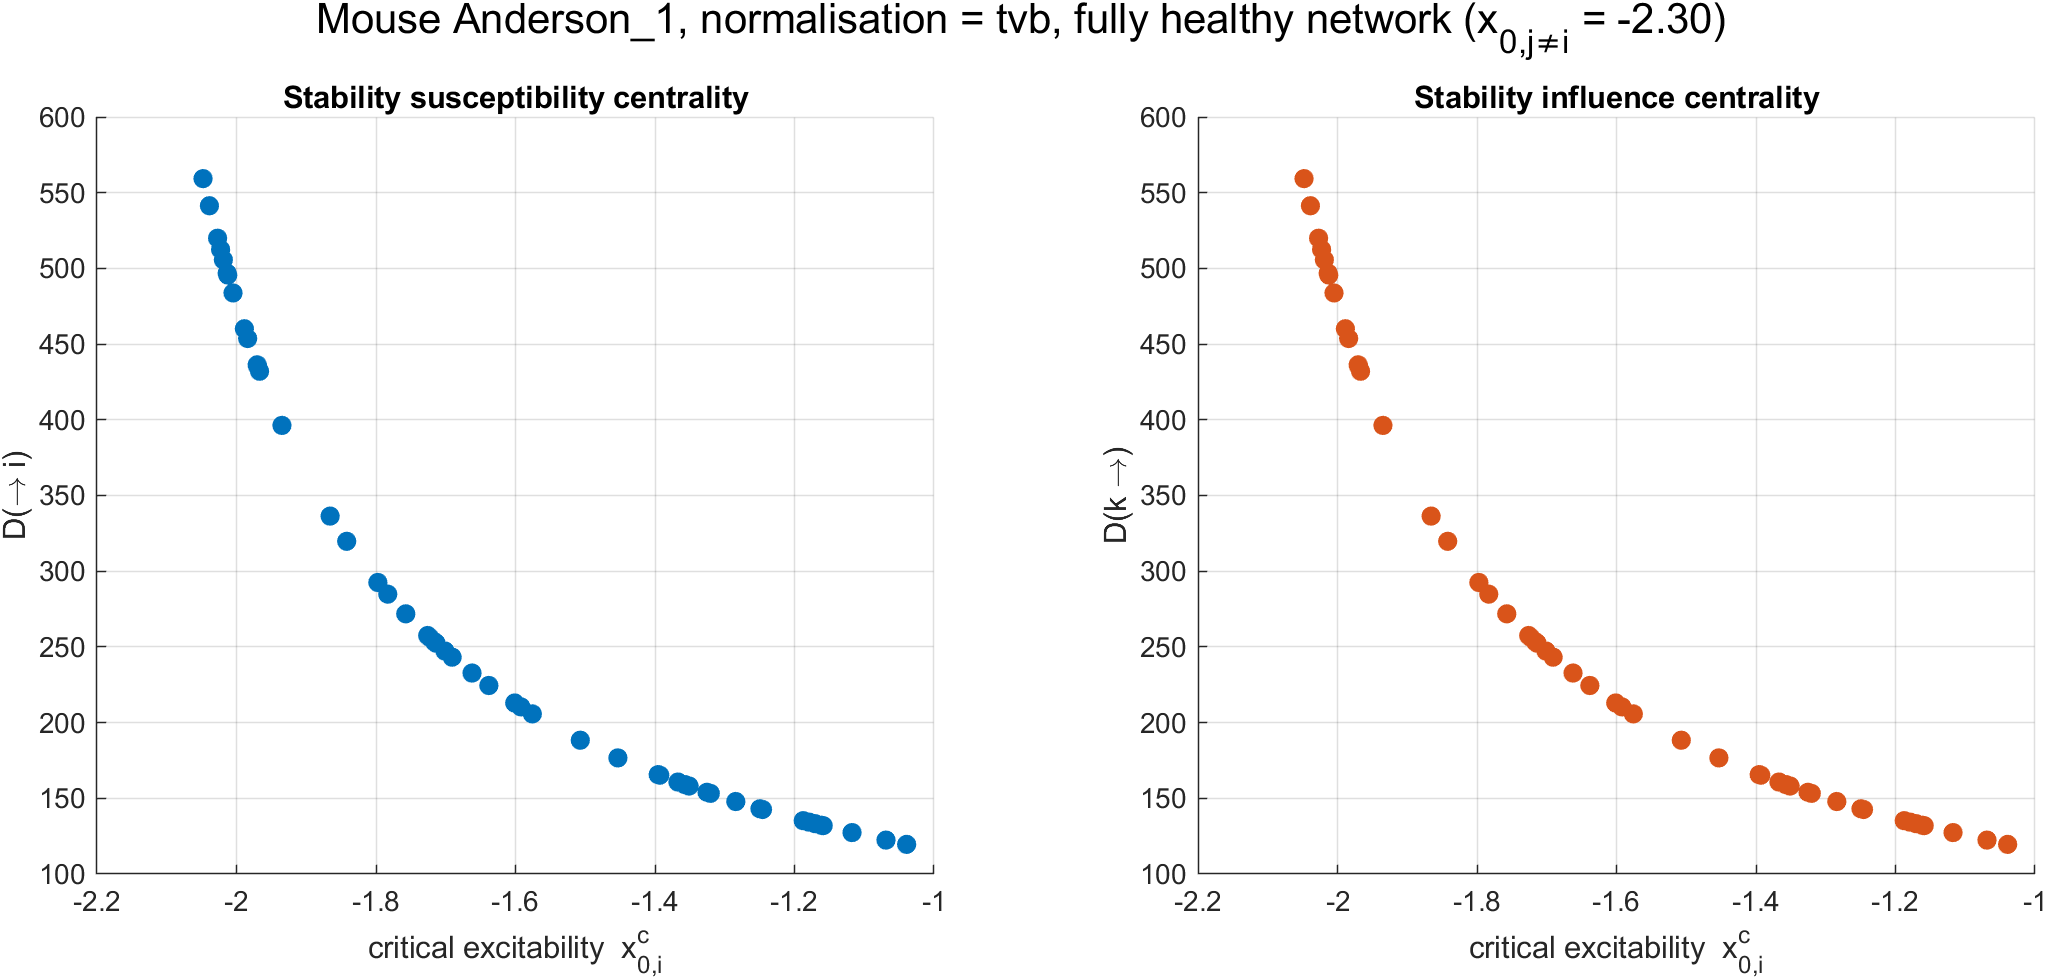
\includegraphics[width=\linewidth]{appendix/stabilityCentralities_Anderson_1_tvb_figure.png}
\caption{\textsc{Anderson\_1}}
\end{subfigure}\hfill
\begin{subfigure}{0.32\textwidth}\centering
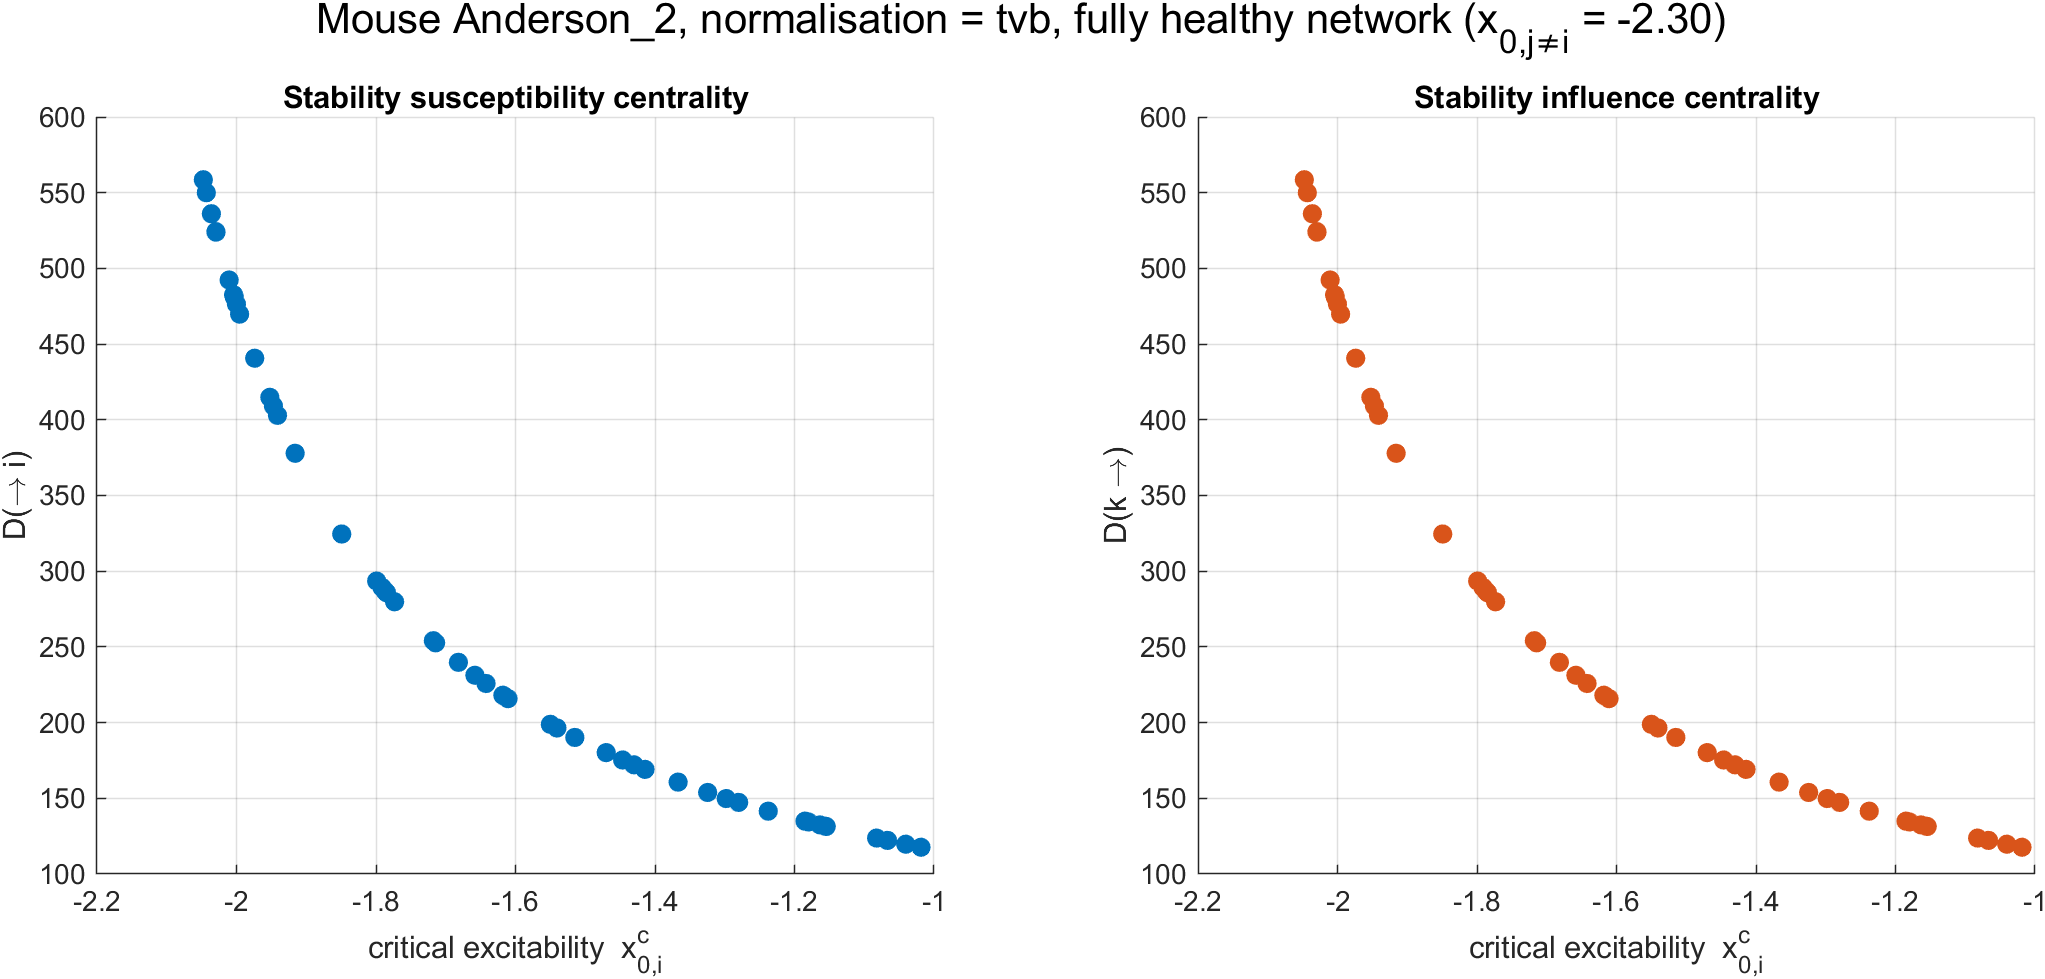
\includegraphics[width=\linewidth]{appendix/stabilityCentralities_Anderson_2_tvb_figure.png}
\caption{\textsc{Anderson\_2}}
\end{subfigure}\hfill
\begin{subfigure}{0.32\textwidth}\centering
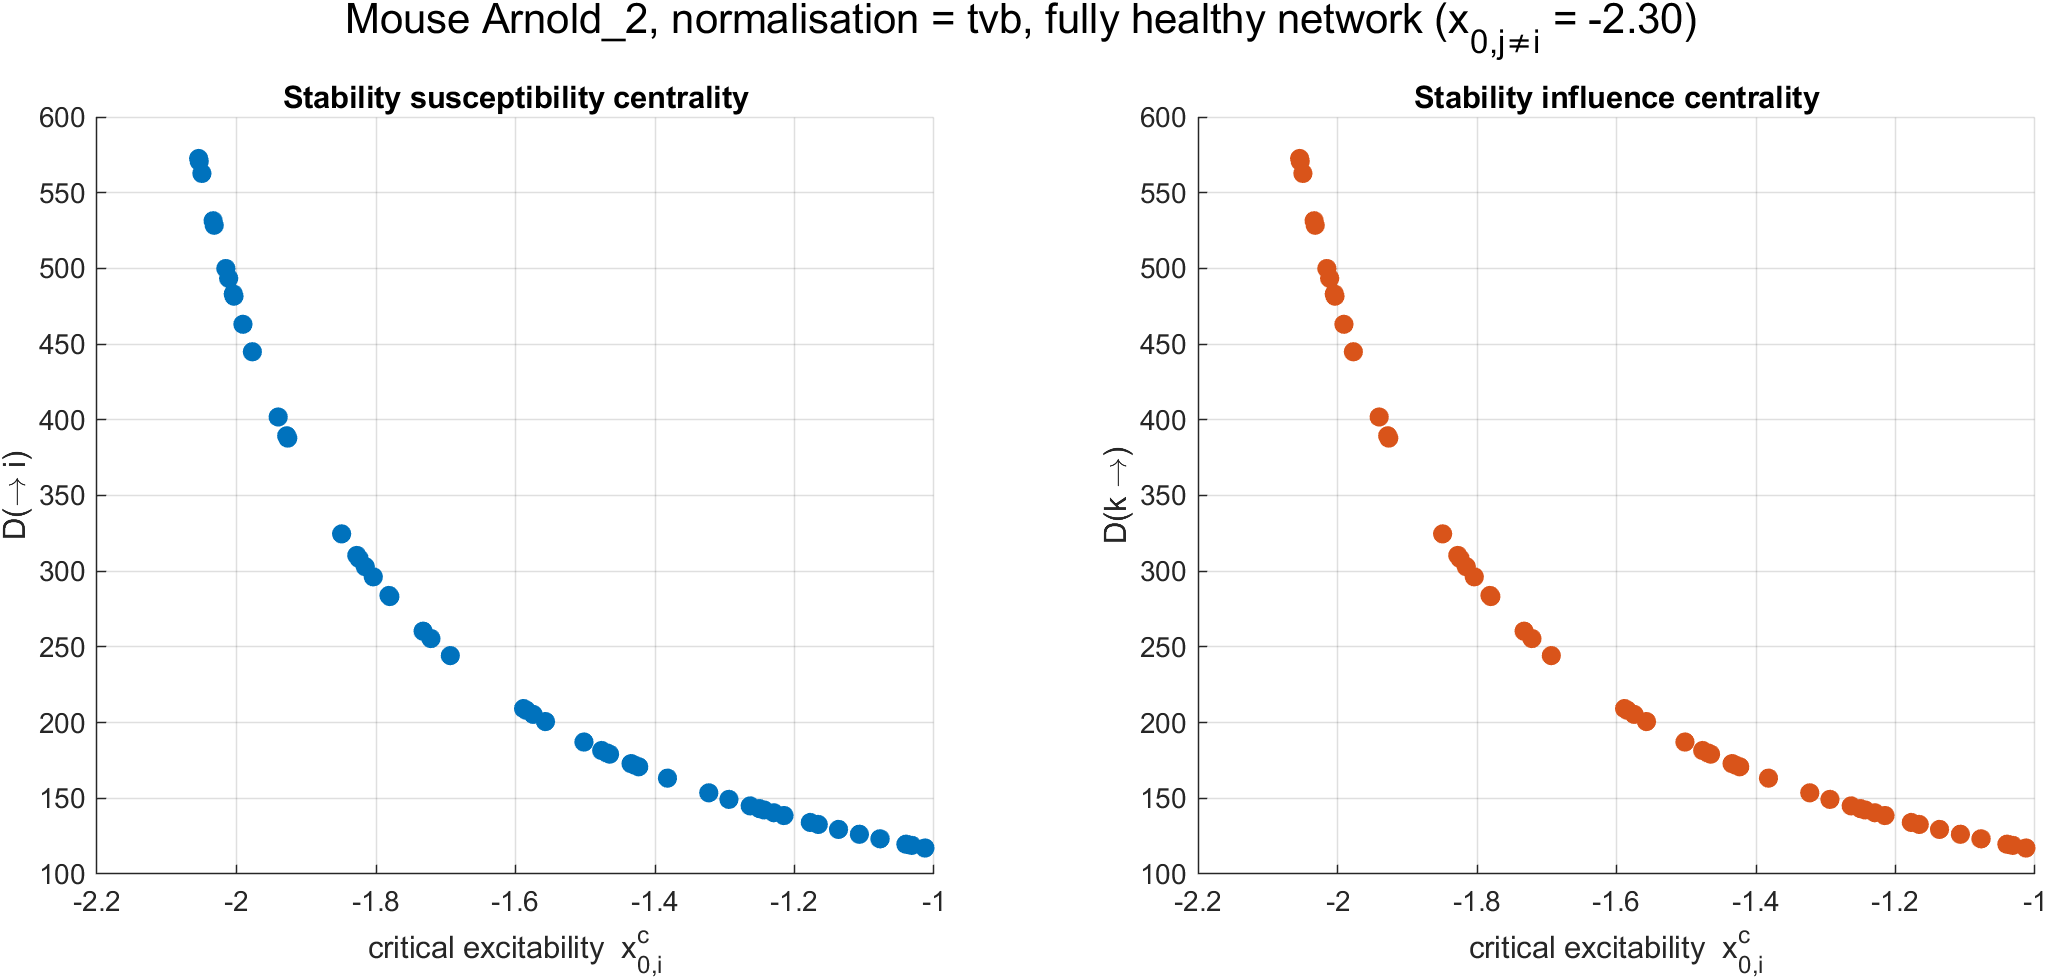
\includegraphics[width=\linewidth]{appendix/stabilityCentralities_Arnold_2_tvb_figure.png}
\caption{\textsc{Arnold\_2}}
\end{subfigure}\hfill
\begin{subfigure}{0.32\textwidth}\centering
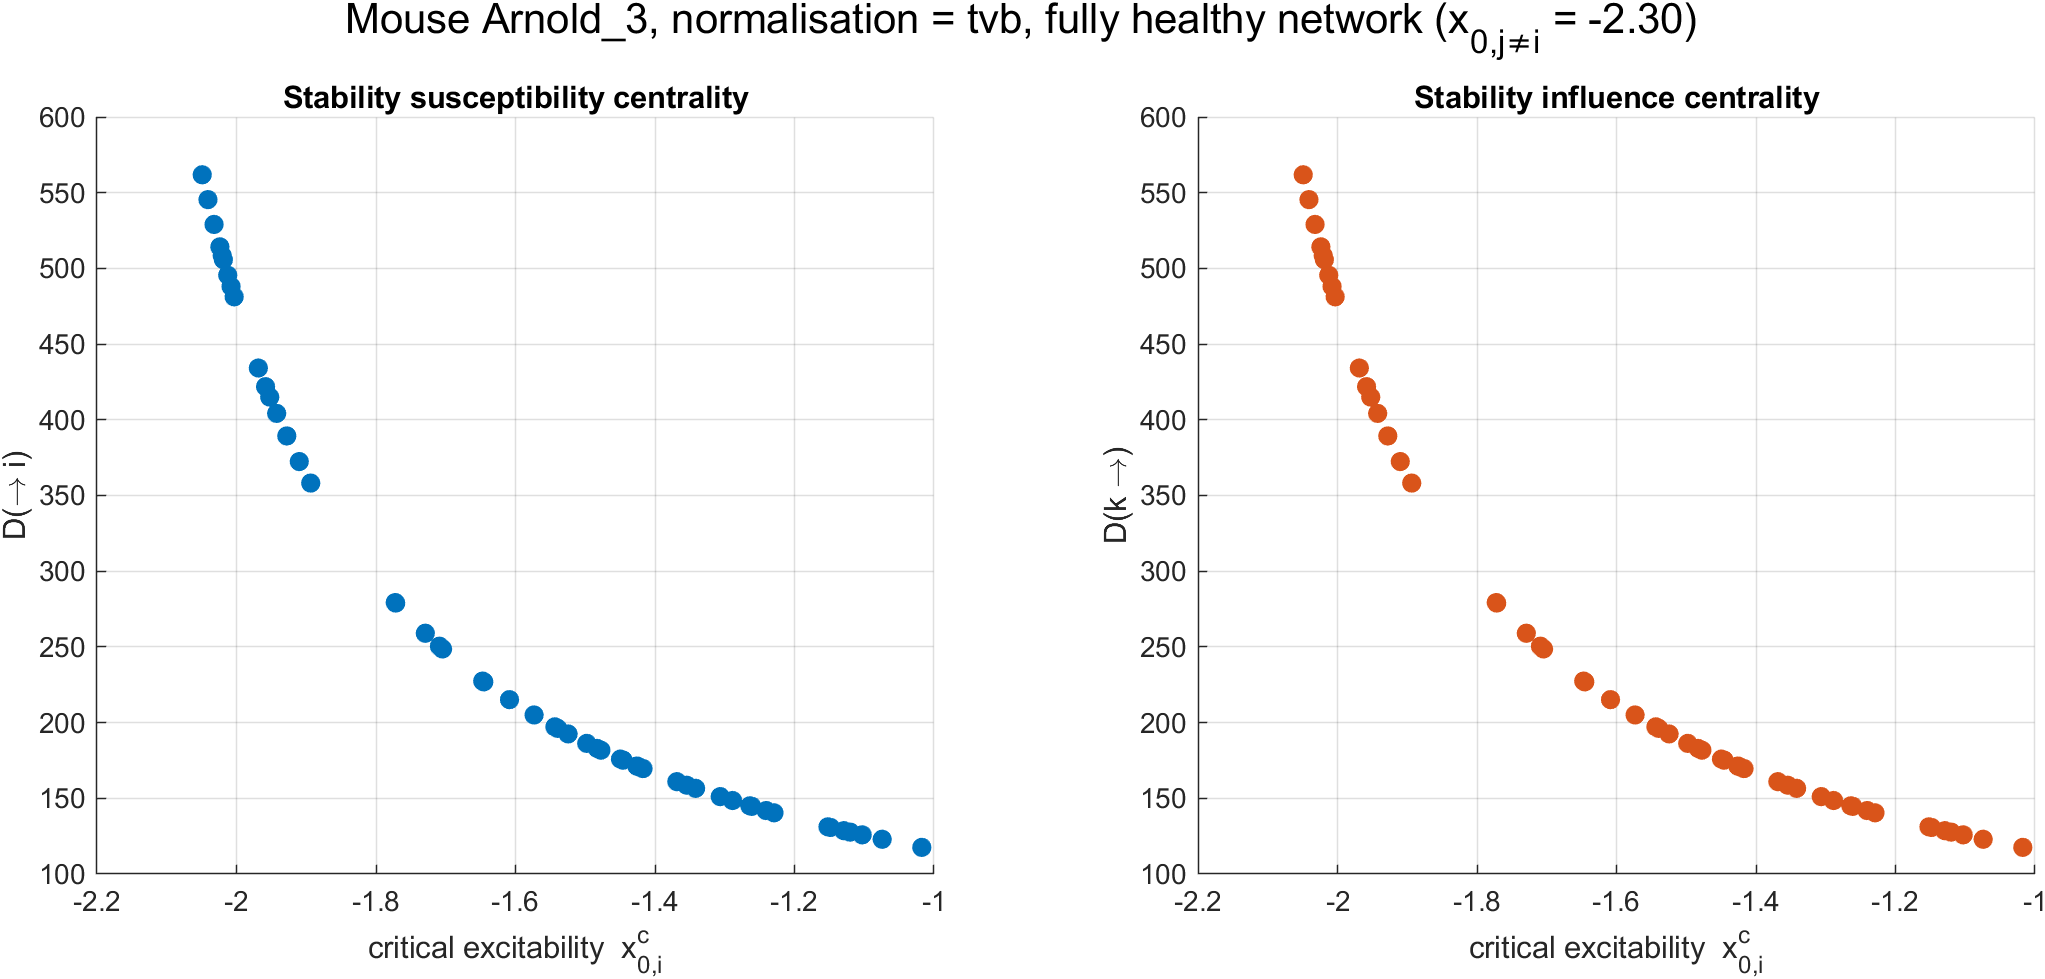
\includegraphics[width=\linewidth]{appendix/stabilityCentralities_Arnold_3_tvb_figure.png}
\caption{\textsc{Arnold\_3}}
\end{subfigure}\hfill
\begin{subfigure}{0.32\textwidth}\centering
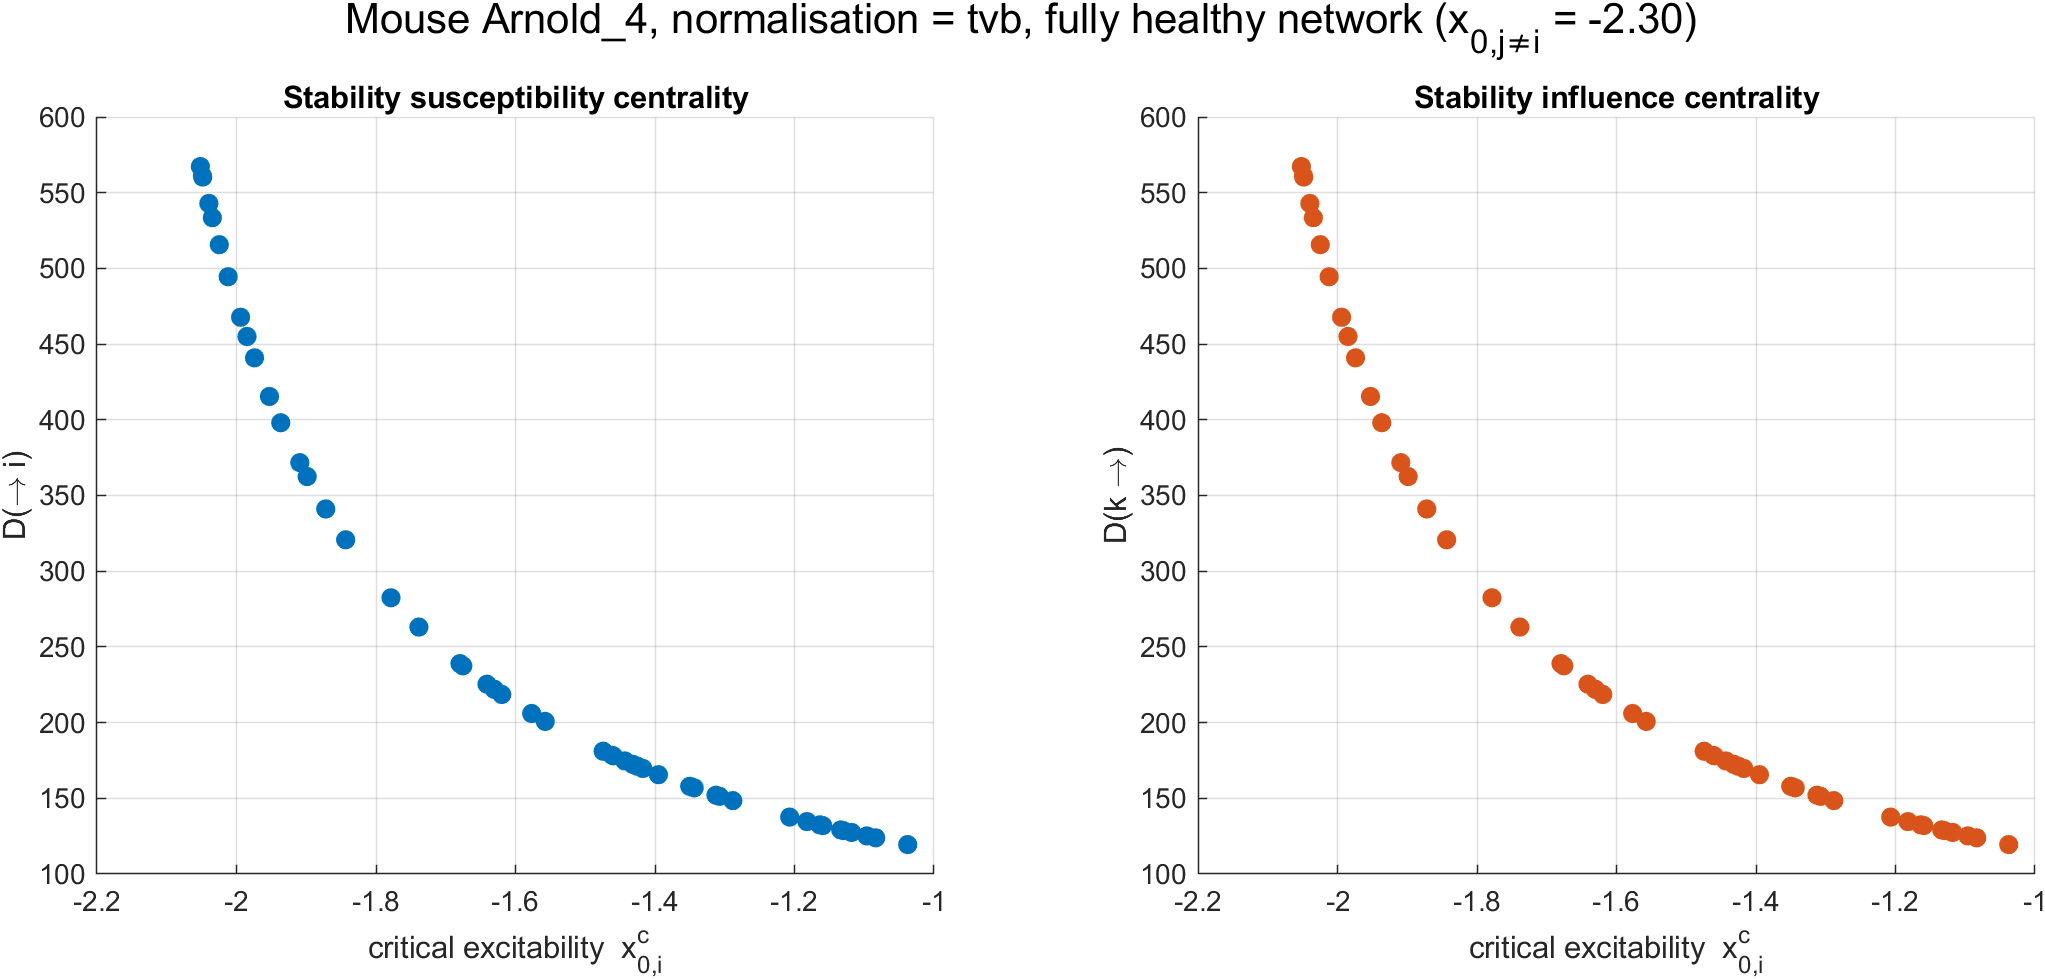
\includegraphics[width=\linewidth]{appendix/stabilityCentralities_Arnold_4_tvb_figure.png}
\caption{\textsc{Arnold\_4}}
\end{subfigure}\hfill
\begin{subfigure}{0.32\textwidth}\centering
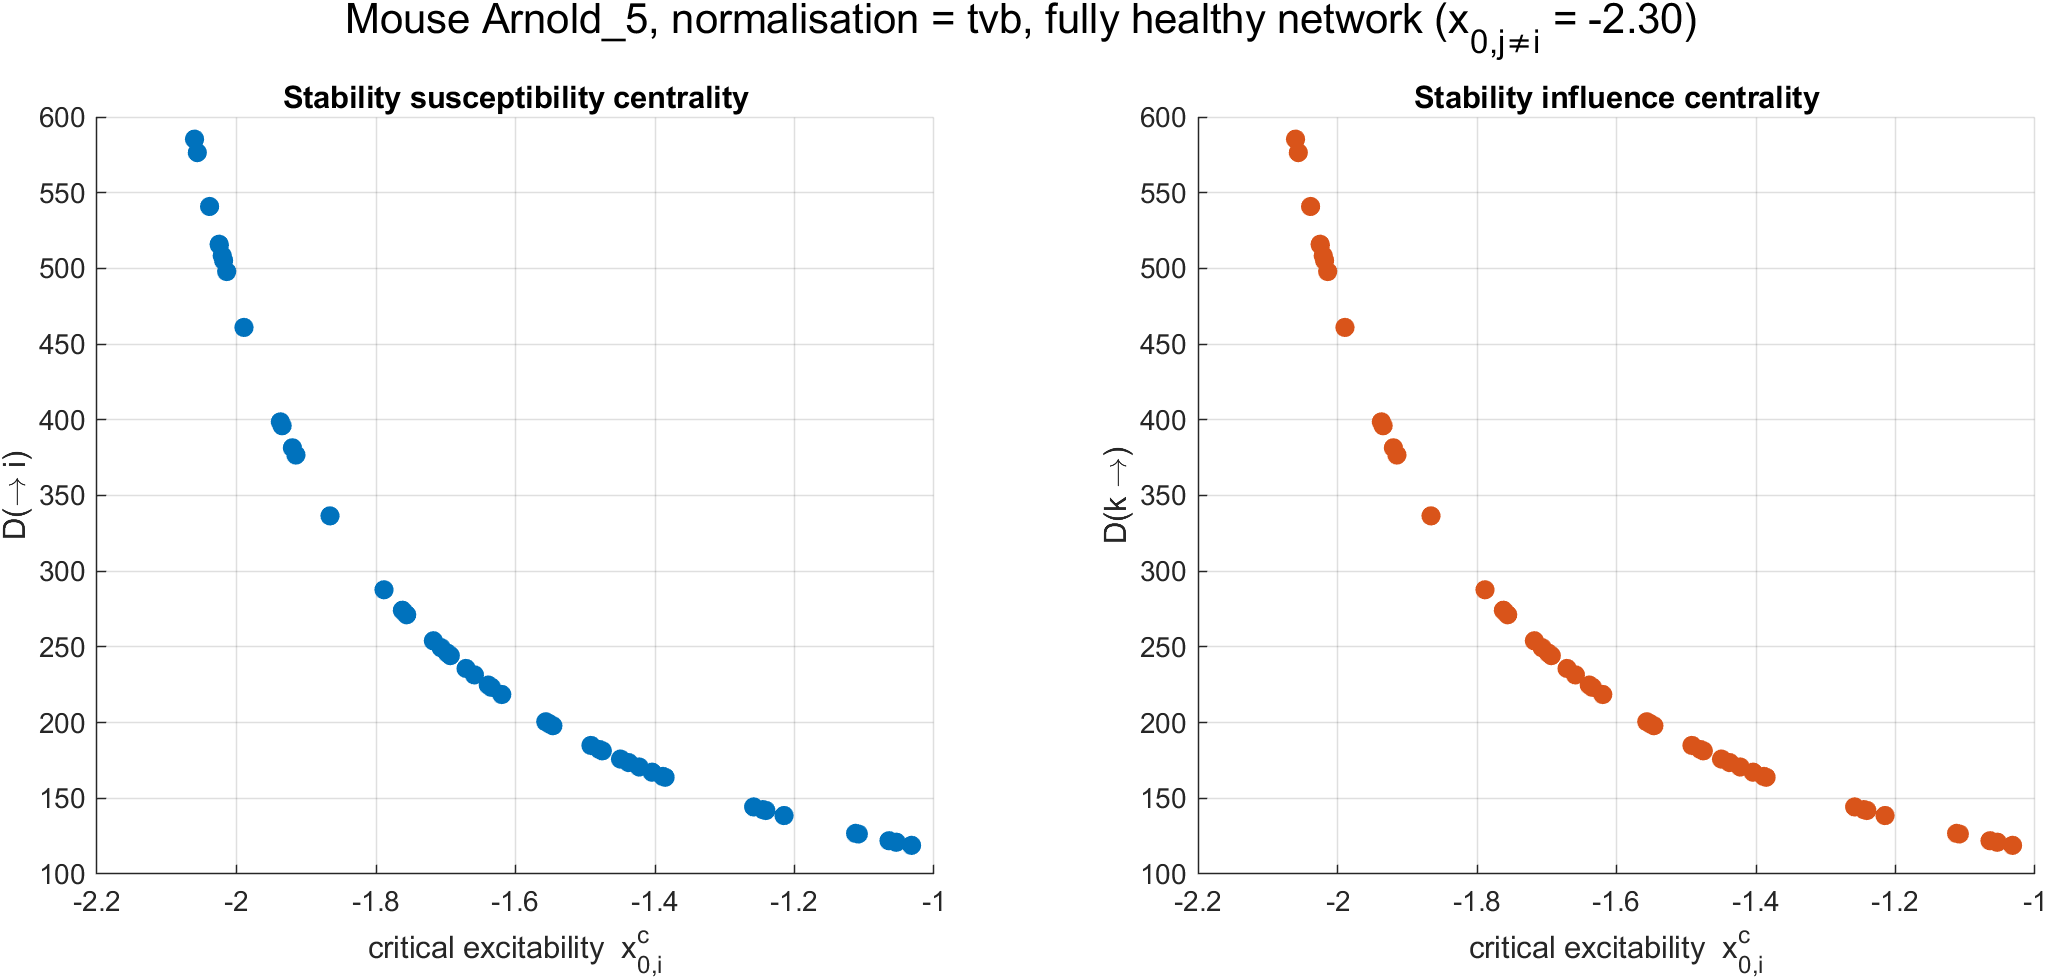
\includegraphics[width=\linewidth]{appendix/stabilityCentralities_Arnold_5_tvb_figure.png}
\caption{\textsc{Arnold\_5}}
\end{subfigure}\hfill
\caption{Per-region susceptibility $\Dto$ and influence $\Dfrom$ for all six mice, \texttt{tvb} scheme.}
\end{figure}
\begin{figure}[H]\centering
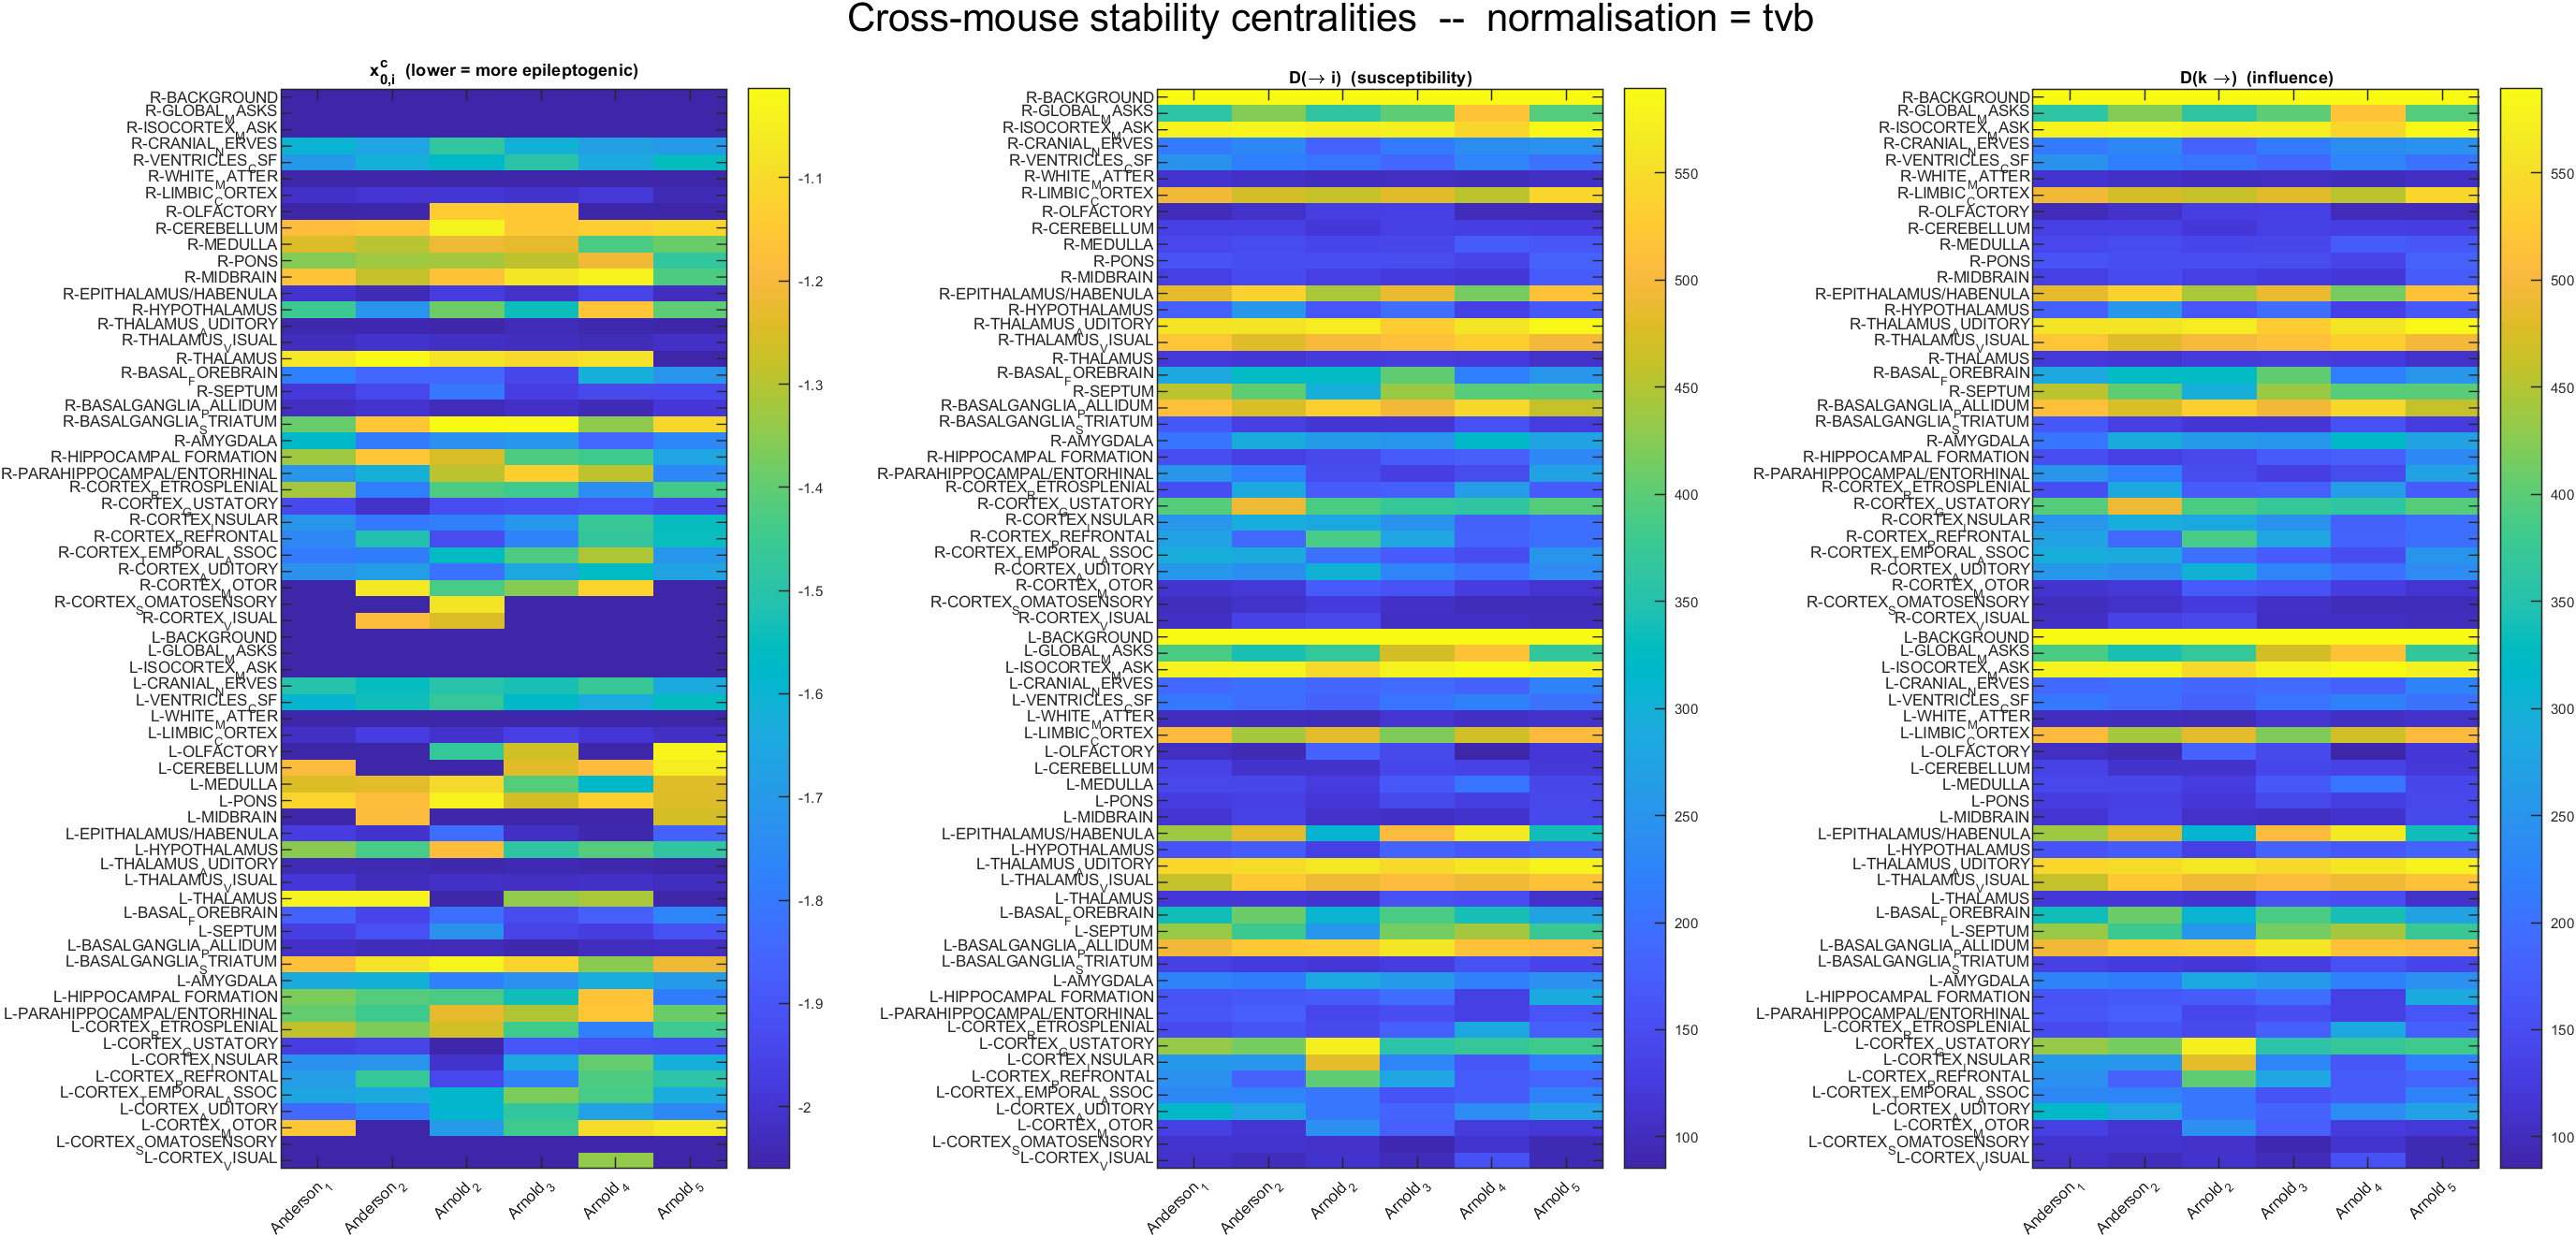
\includegraphics[width=0.8\textwidth]{appendix/stabilityCentralities_summary_overview_tvb.png}
\caption{Cohort overview of stability centralities, \texttt{tvb} scheme.}
\end{figure}

\subsection{Centrality correlations}
\begin{figure}[H]\centering
\begin{subfigure}{0.48\textwidth}\centering
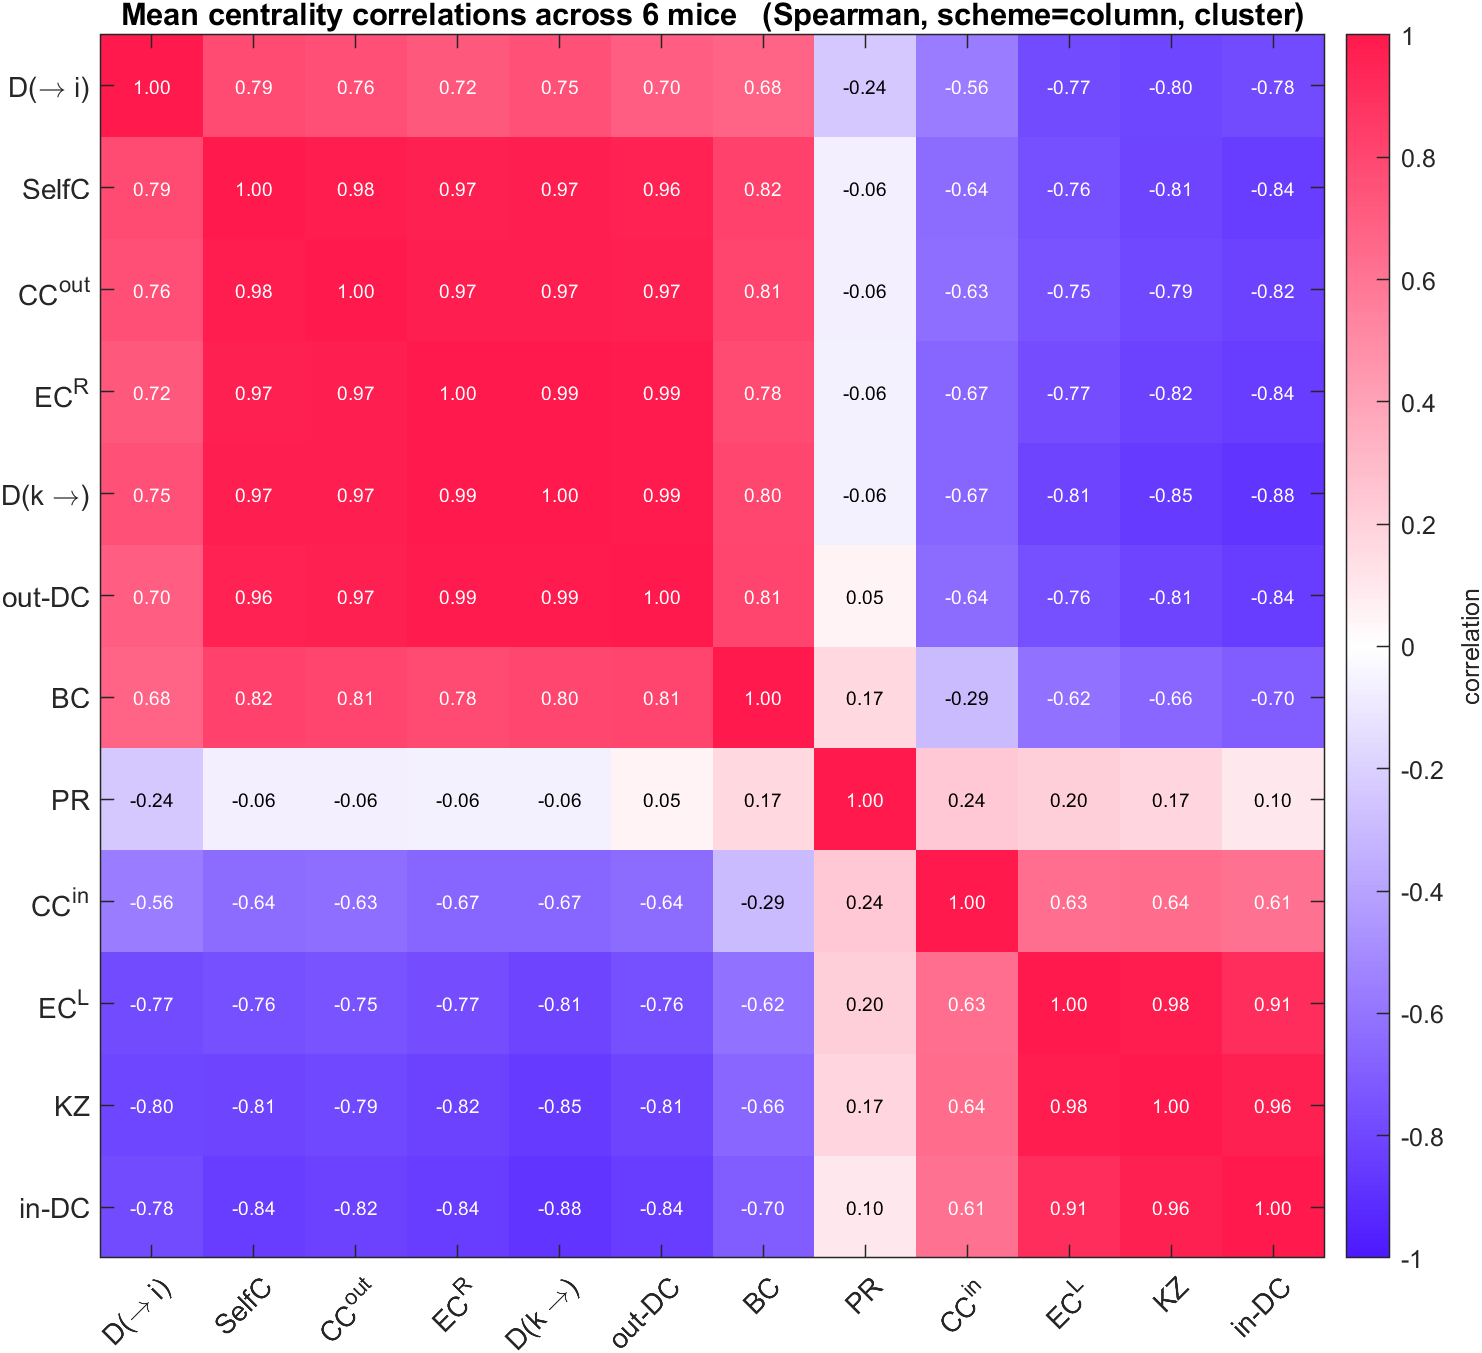
\includegraphics[width=\linewidth]{appendix/centrality_corr_mean_column.png}
\caption{Cohort mean}
\end{subfigure}\hfill
\begin{subfigure}{0.48\textwidth}\centering
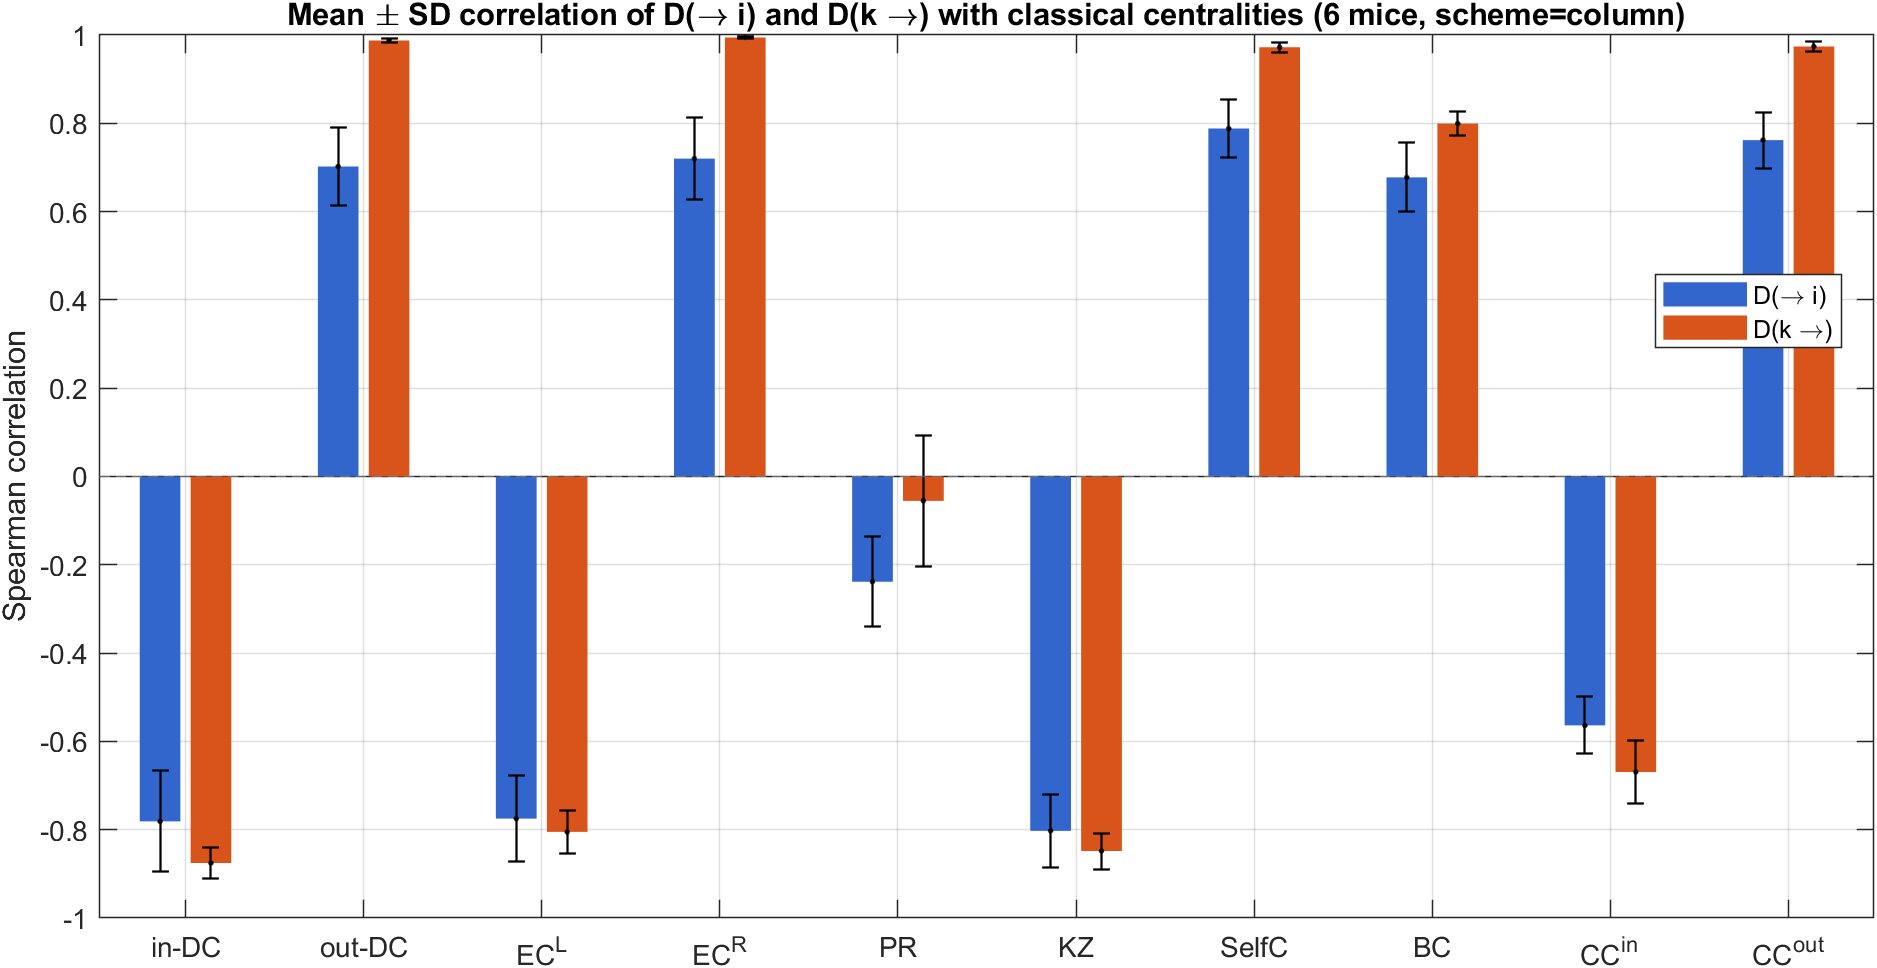
\includegraphics[width=\linewidth]{appendix/centrality_corr_bars_column.png}
\caption{$\Dto$, $\Dfrom$ vs classical}
\end{subfigure}
\caption{Centrality correlation summary, \texttt{column} scheme.}
\end{figure}
\begin{figure}[H]\centering
\begin{subfigure}{0.32\textwidth}\centering
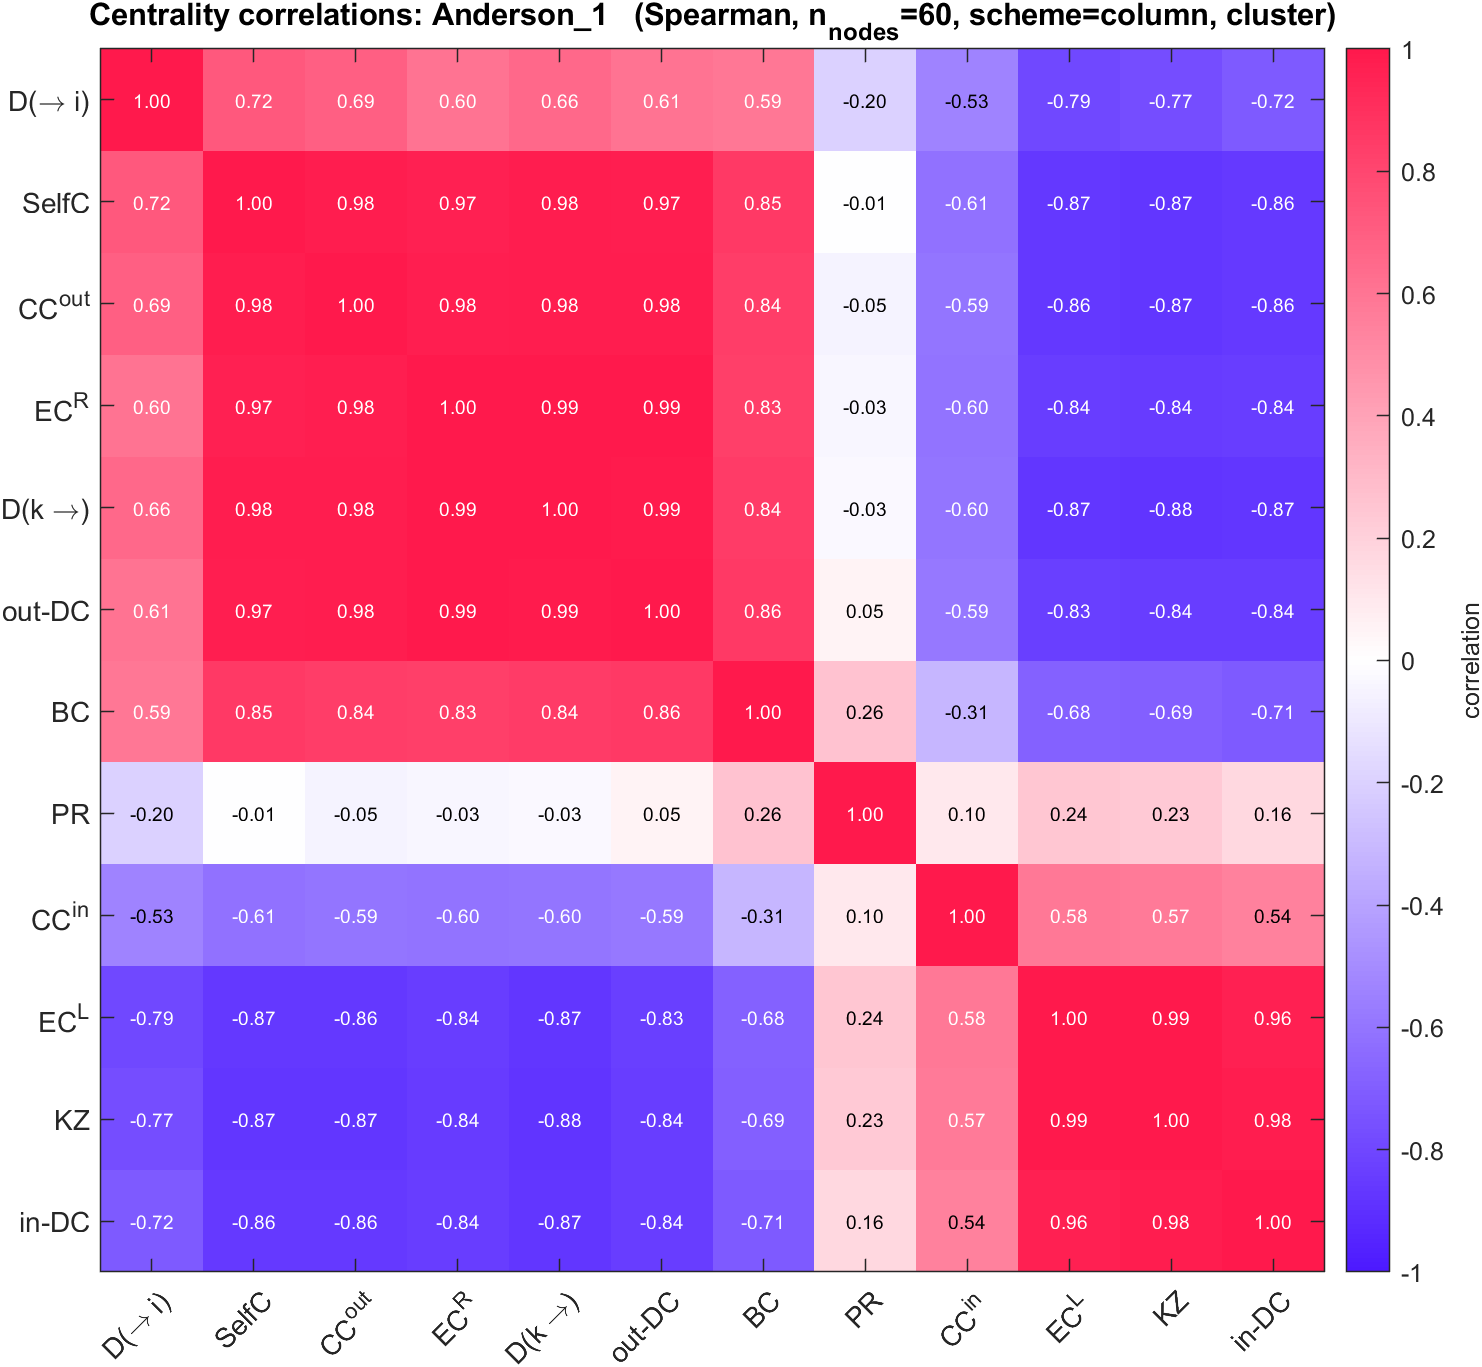
\includegraphics[width=\linewidth]{appendix/centrality_corr_Anderson_1_column.png}
\caption{\textsc{Anderson\_1}}
\end{subfigure}\hfill
\begin{subfigure}{0.32\textwidth}\centering
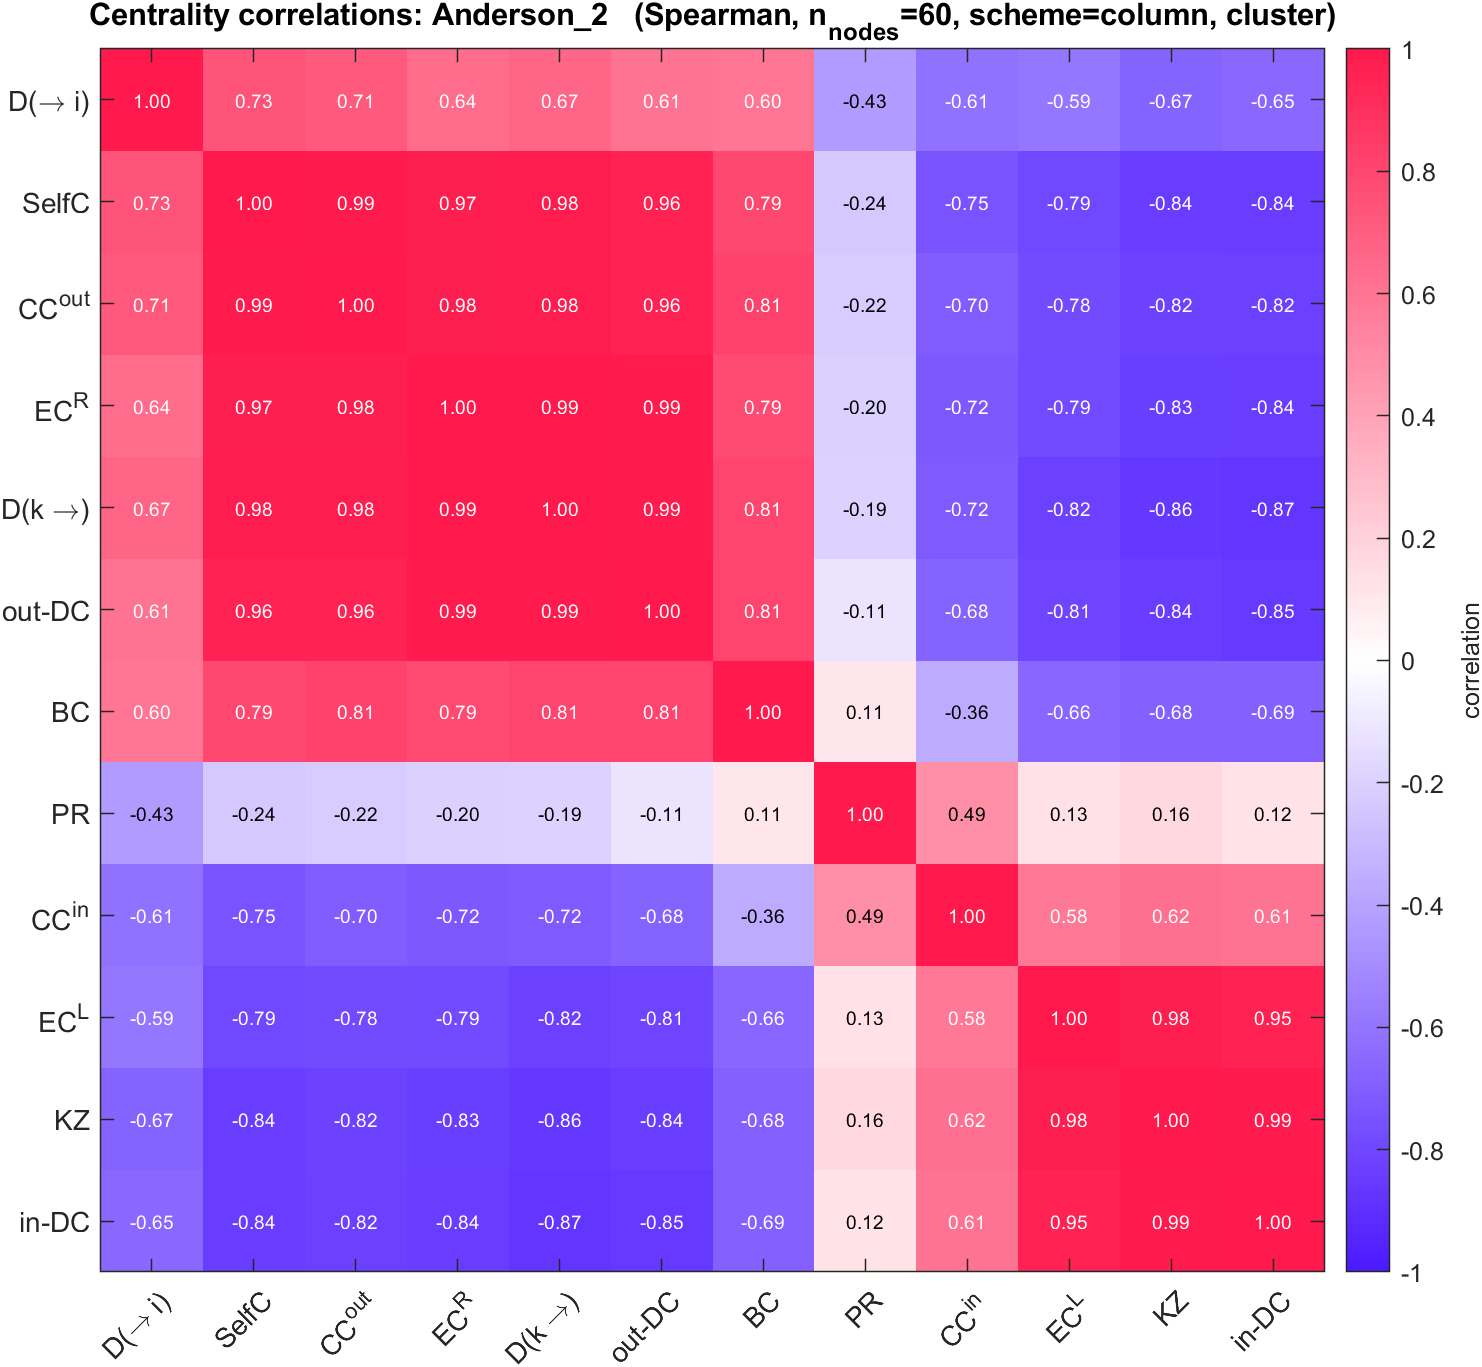
\includegraphics[width=\linewidth]{appendix/centrality_corr_Anderson_2_column.png}
\caption{\textsc{Anderson\_2}}
\end{subfigure}\hfill
\begin{subfigure}{0.32\textwidth}\centering
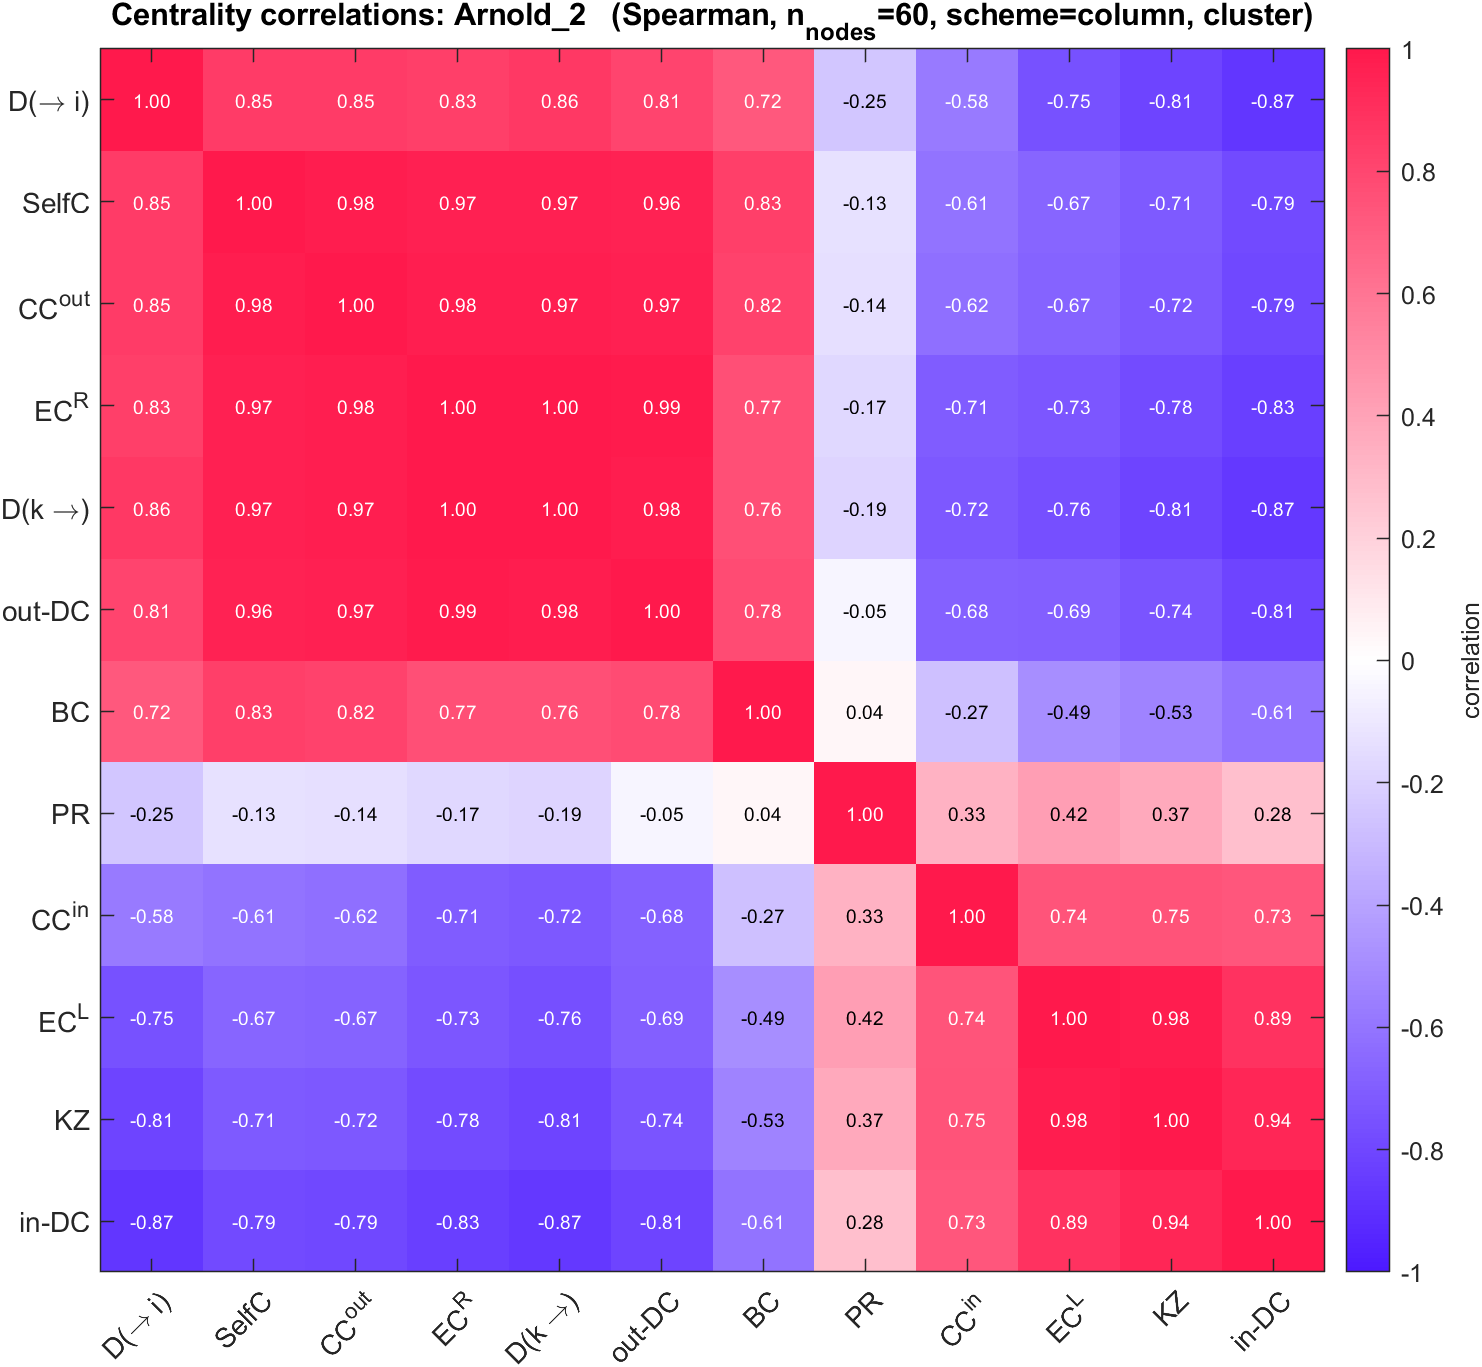
\includegraphics[width=\linewidth]{appendix/centrality_corr_Arnold_2_column.png}
\caption{\textsc{Arnold\_2}}
\end{subfigure}\hfill
\begin{subfigure}{0.32\textwidth}\centering
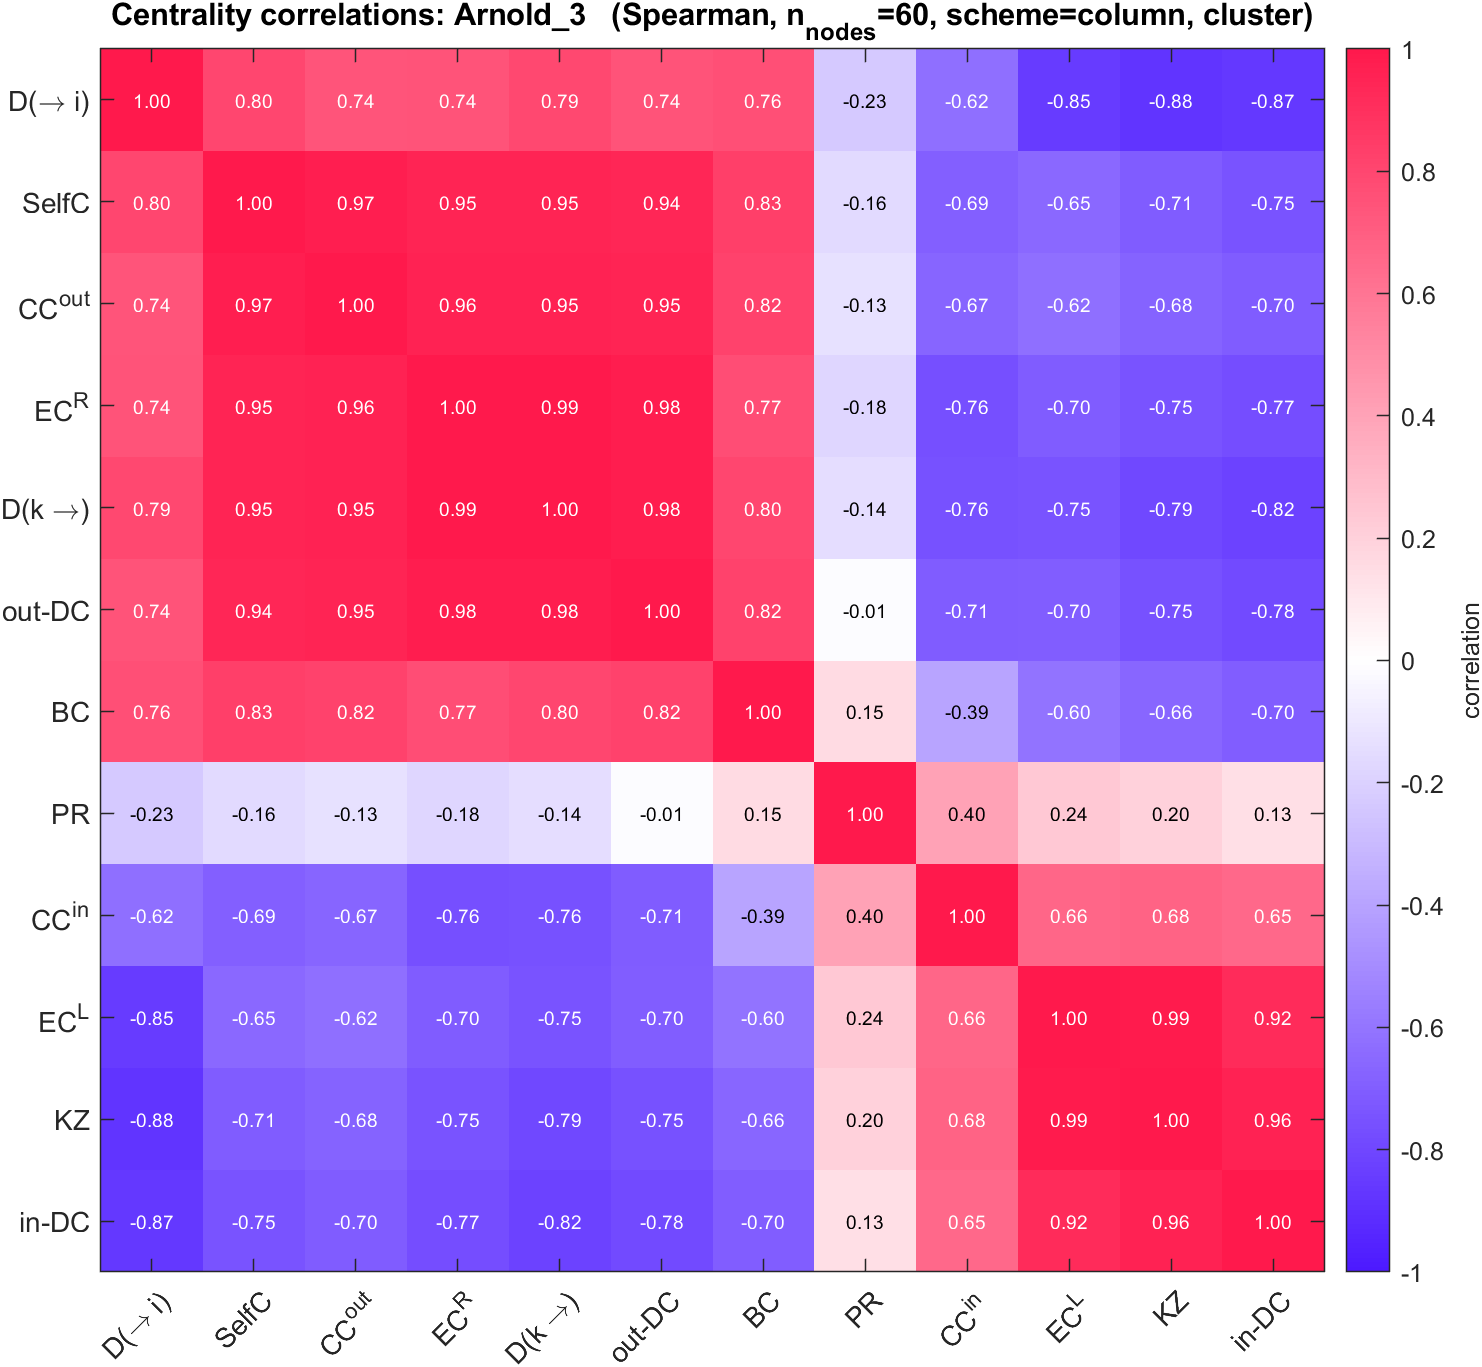
\includegraphics[width=\linewidth]{appendix/centrality_corr_Arnold_3_column.png}
\caption{\textsc{Arnold\_3}}
\end{subfigure}\hfill
\begin{subfigure}{0.32\textwidth}\centering
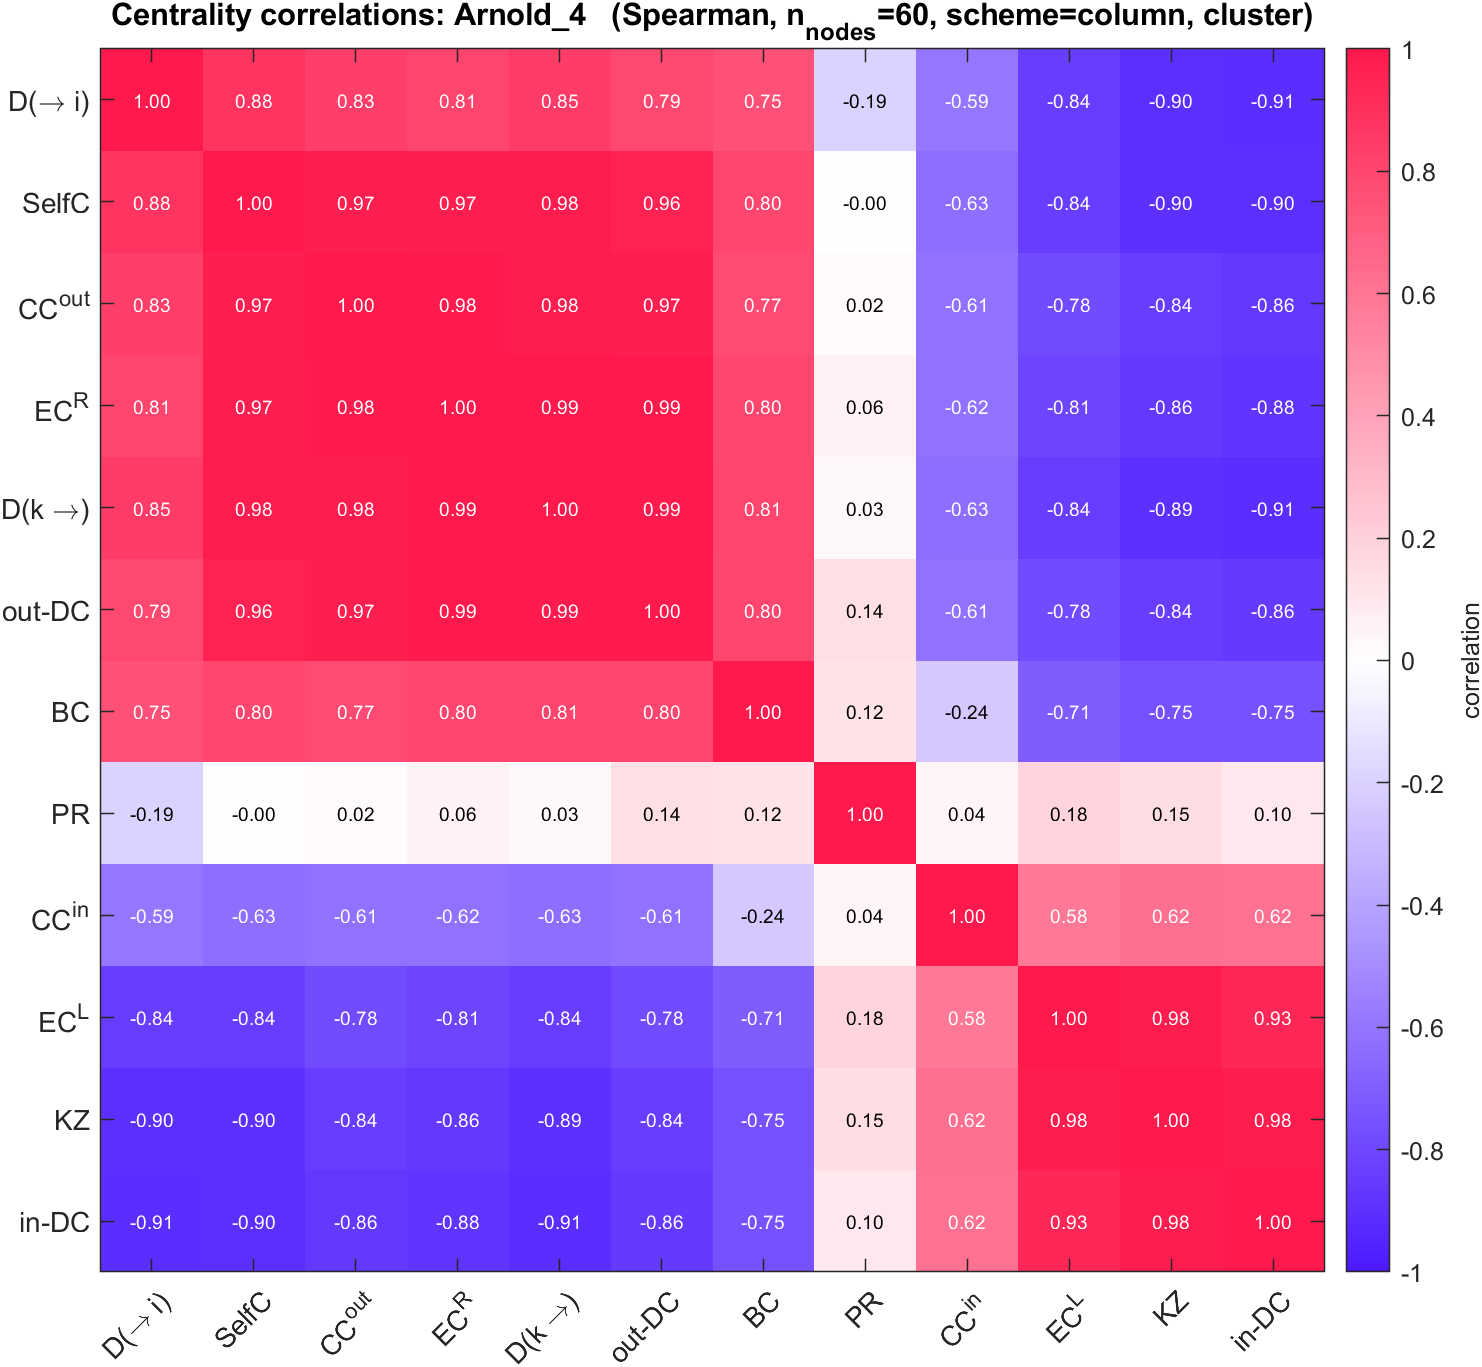
\includegraphics[width=\linewidth]{appendix/centrality_corr_Arnold_4_column.png}
\caption{\textsc{Arnold\_4}}
\end{subfigure}\hfill
\begin{subfigure}{0.32\textwidth}\centering
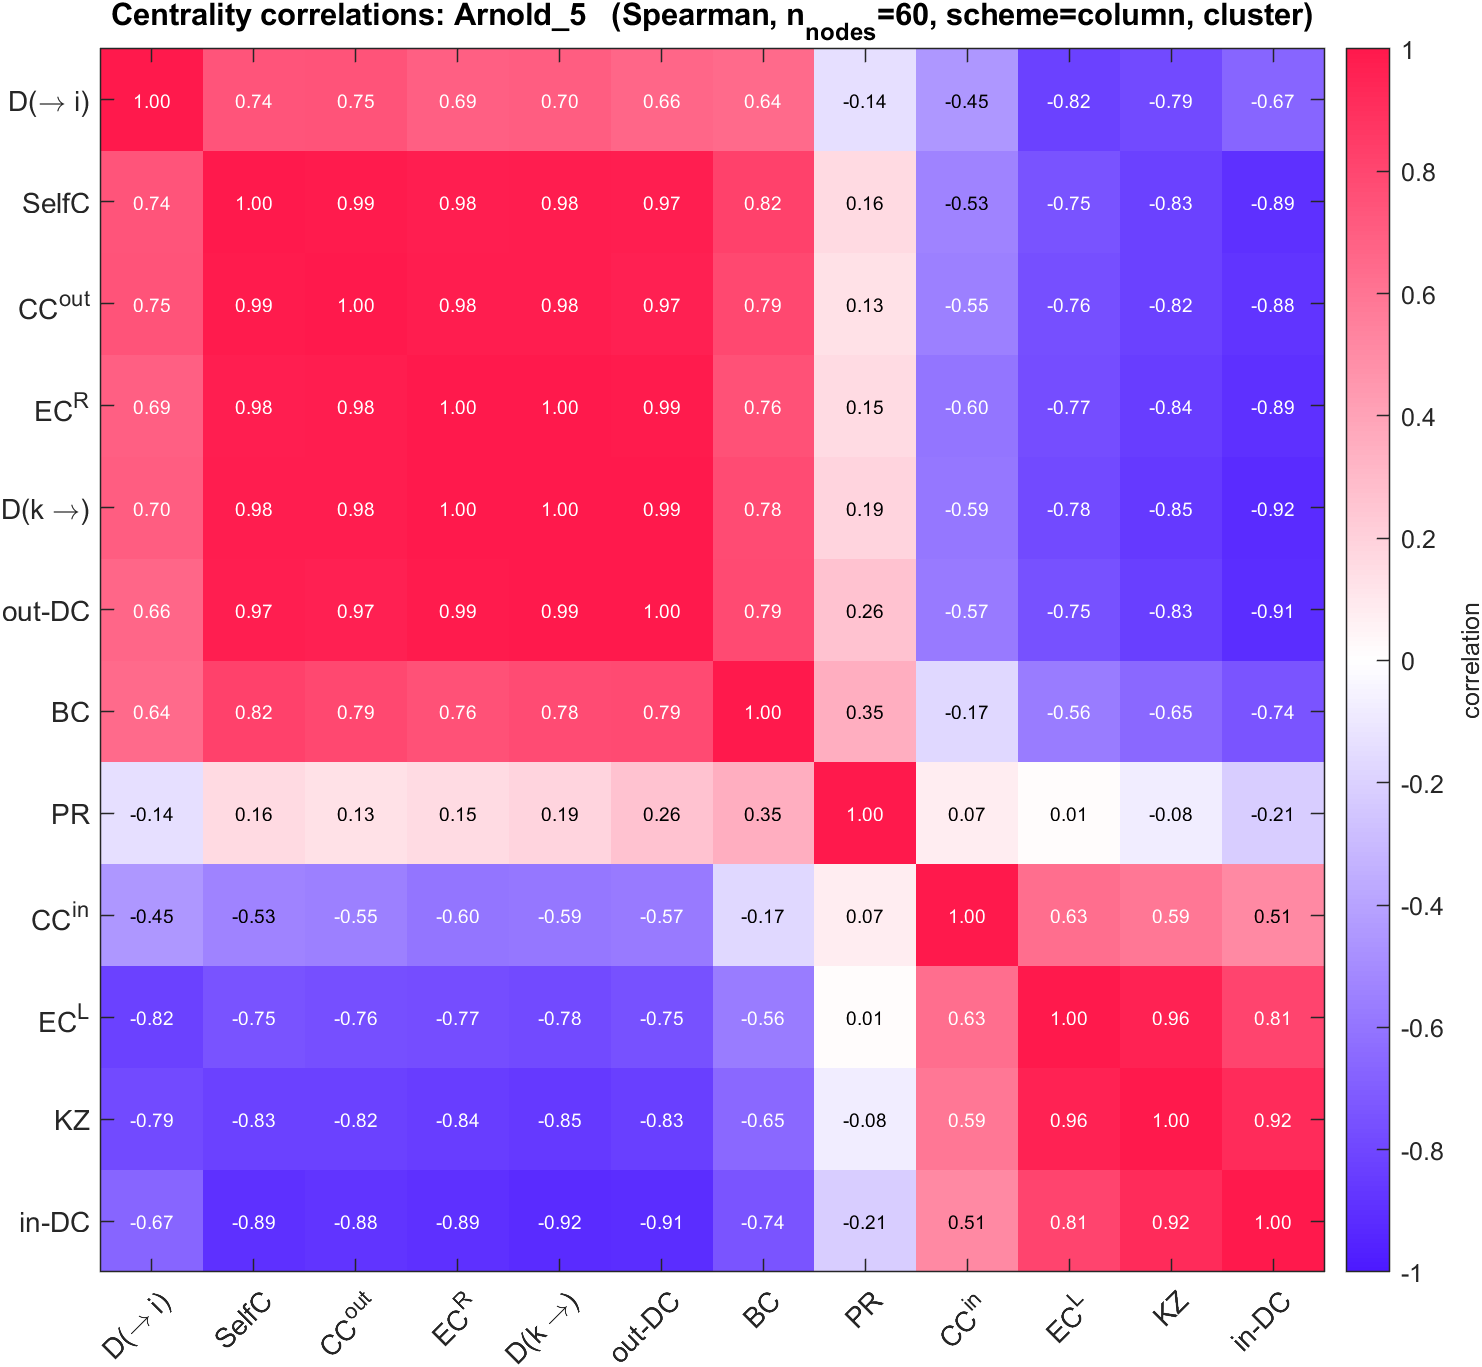
\includegraphics[width=\linewidth]{appendix/centrality_corr_Arnold_5_column.png}
\caption{\textsc{Arnold\_5}}
\end{subfigure}\hfill
\caption{Per-mouse centrality correlation matrices, \texttt{column} scheme.}
\end{figure}

\begin{figure}[H]\centering
\begin{subfigure}{0.48\textwidth}\centering
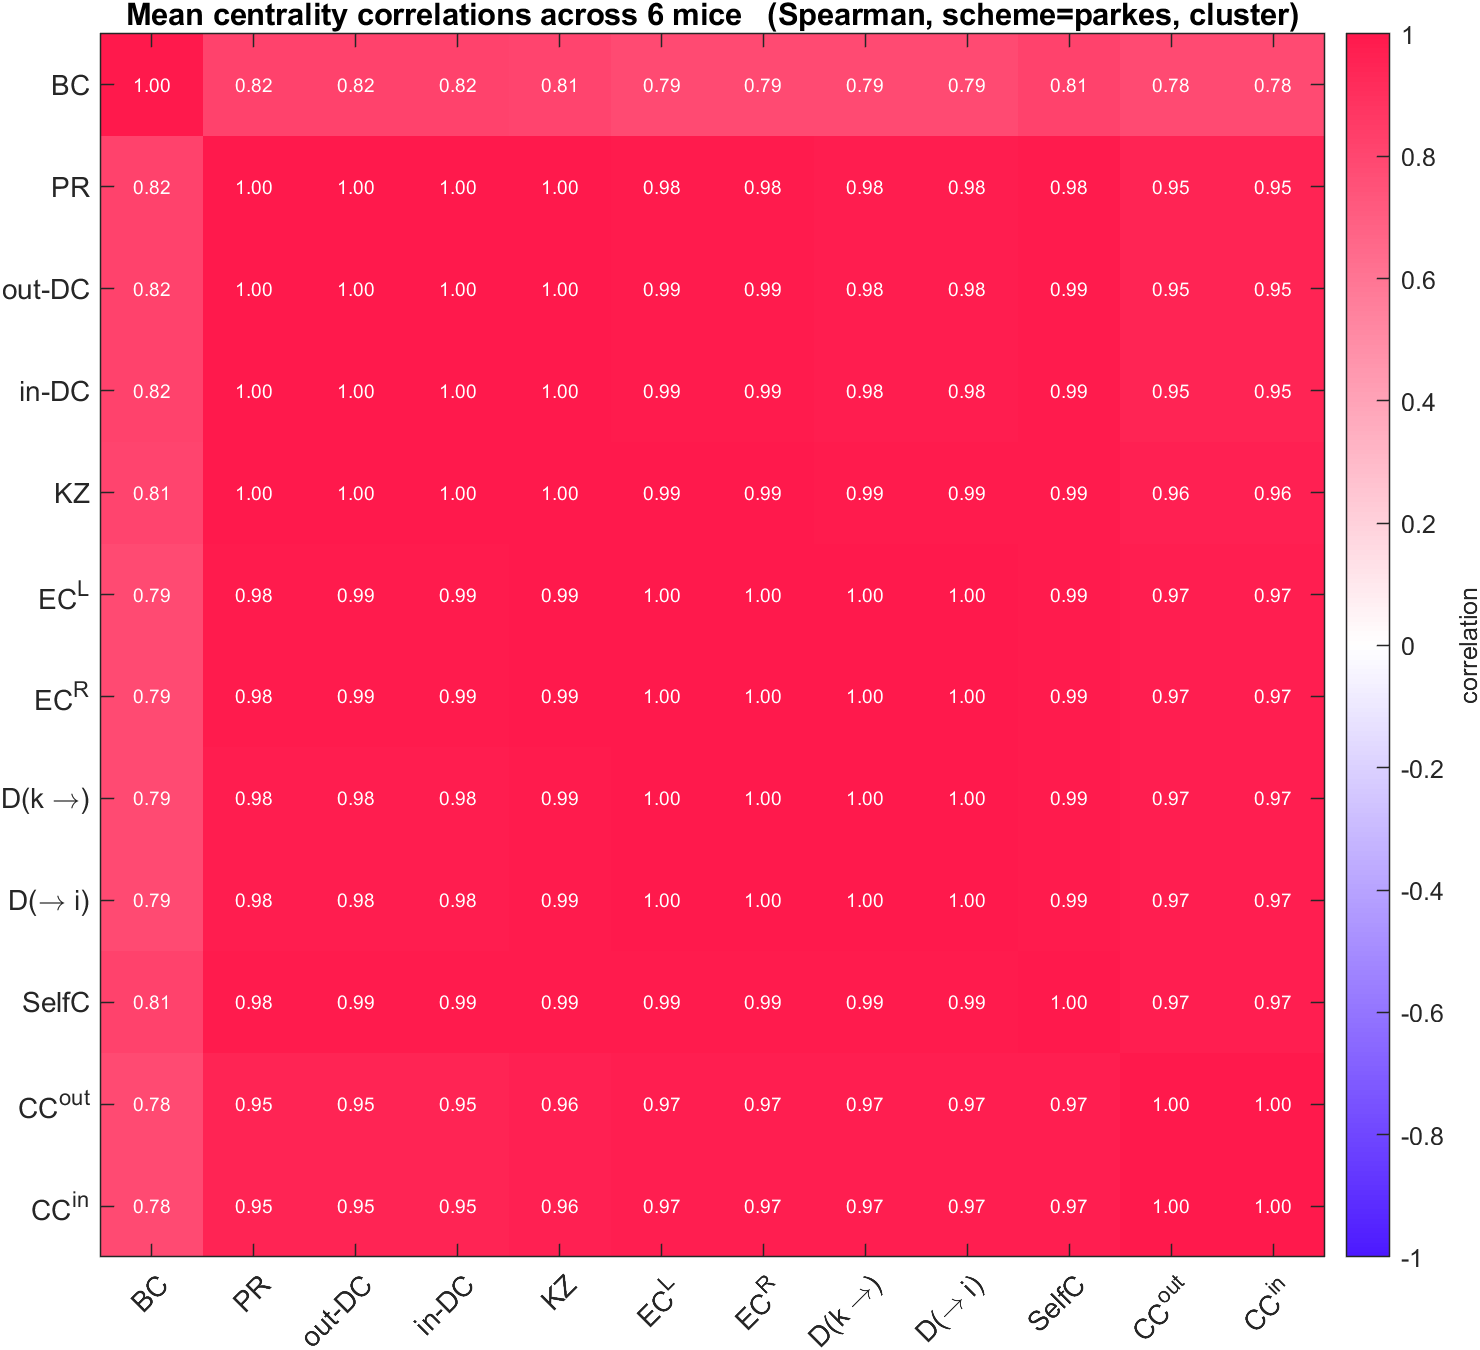
\includegraphics[width=\linewidth]{appendix/centrality_corr_mean_parkes.png}
\caption{Cohort mean}
\end{subfigure}\hfill
\begin{subfigure}{0.48\textwidth}\centering
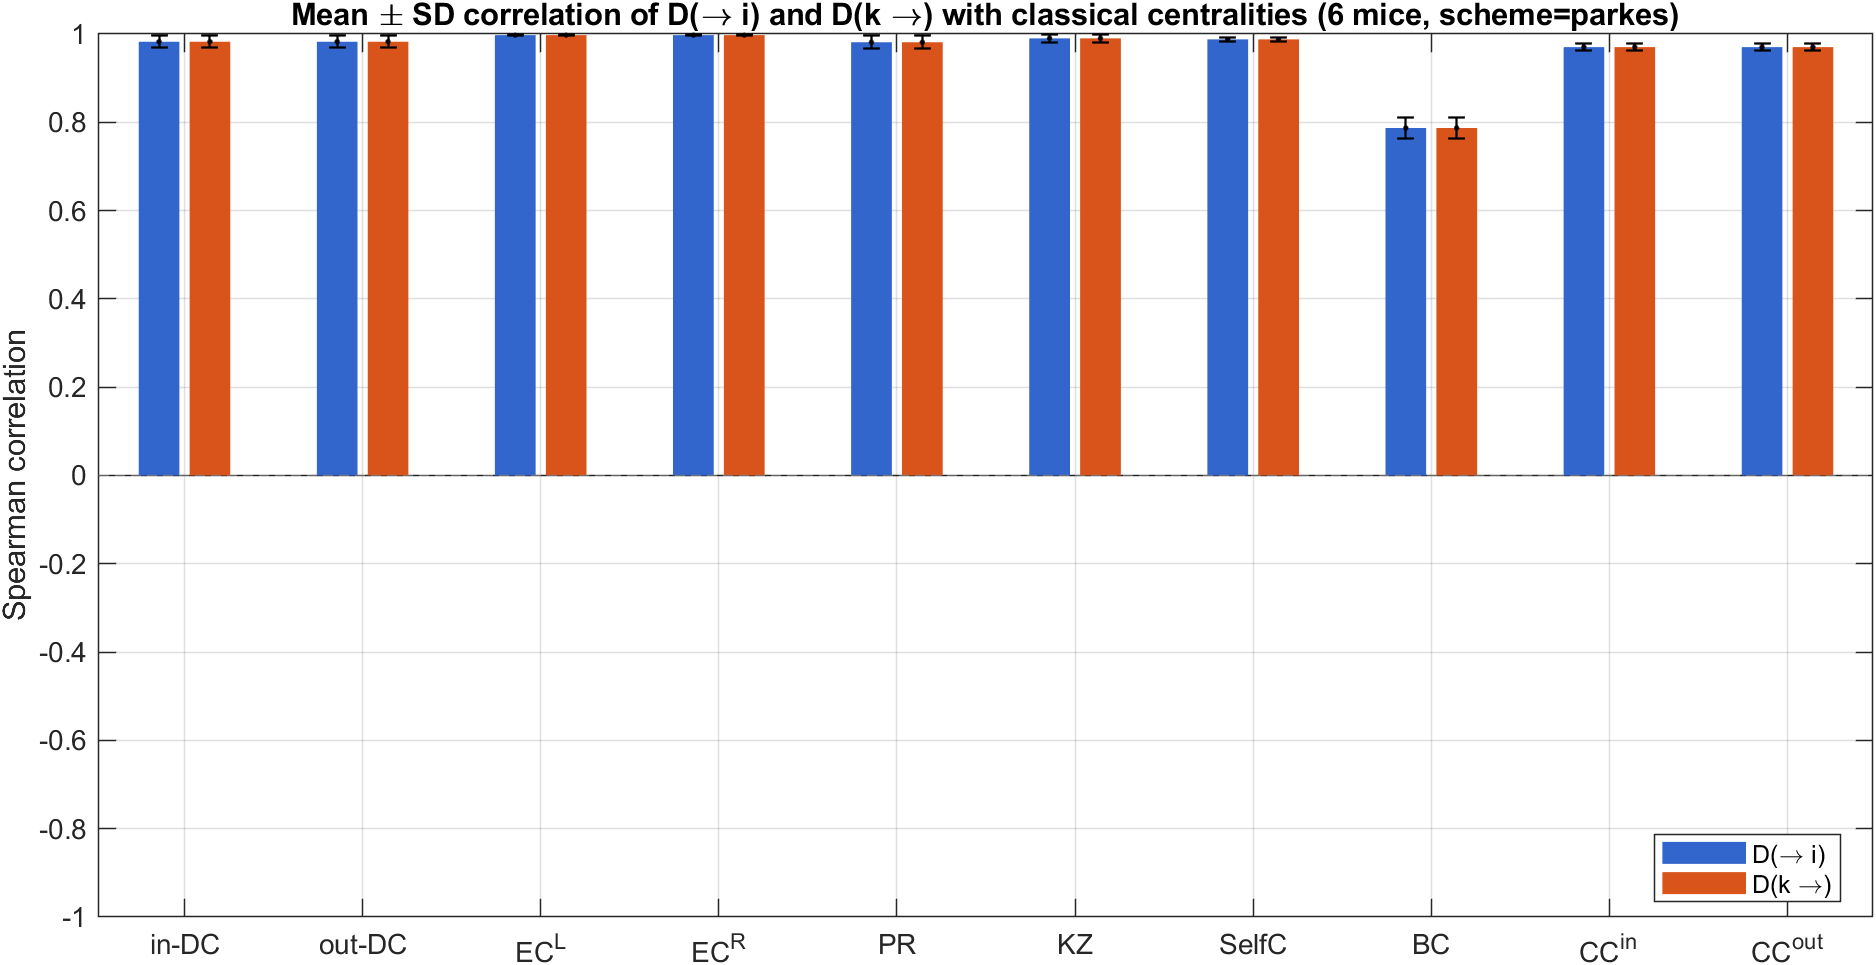
\includegraphics[width=\linewidth]{appendix/centrality_corr_bars_parkes.png}
\caption{$\Dto$, $\Dfrom$ vs classical}
\end{subfigure}
\caption{Centrality correlation summary, \texttt{parkes} scheme.}
\end{figure}
\begin{figure}[H]\centering
\begin{subfigure}{0.32\textwidth}\centering
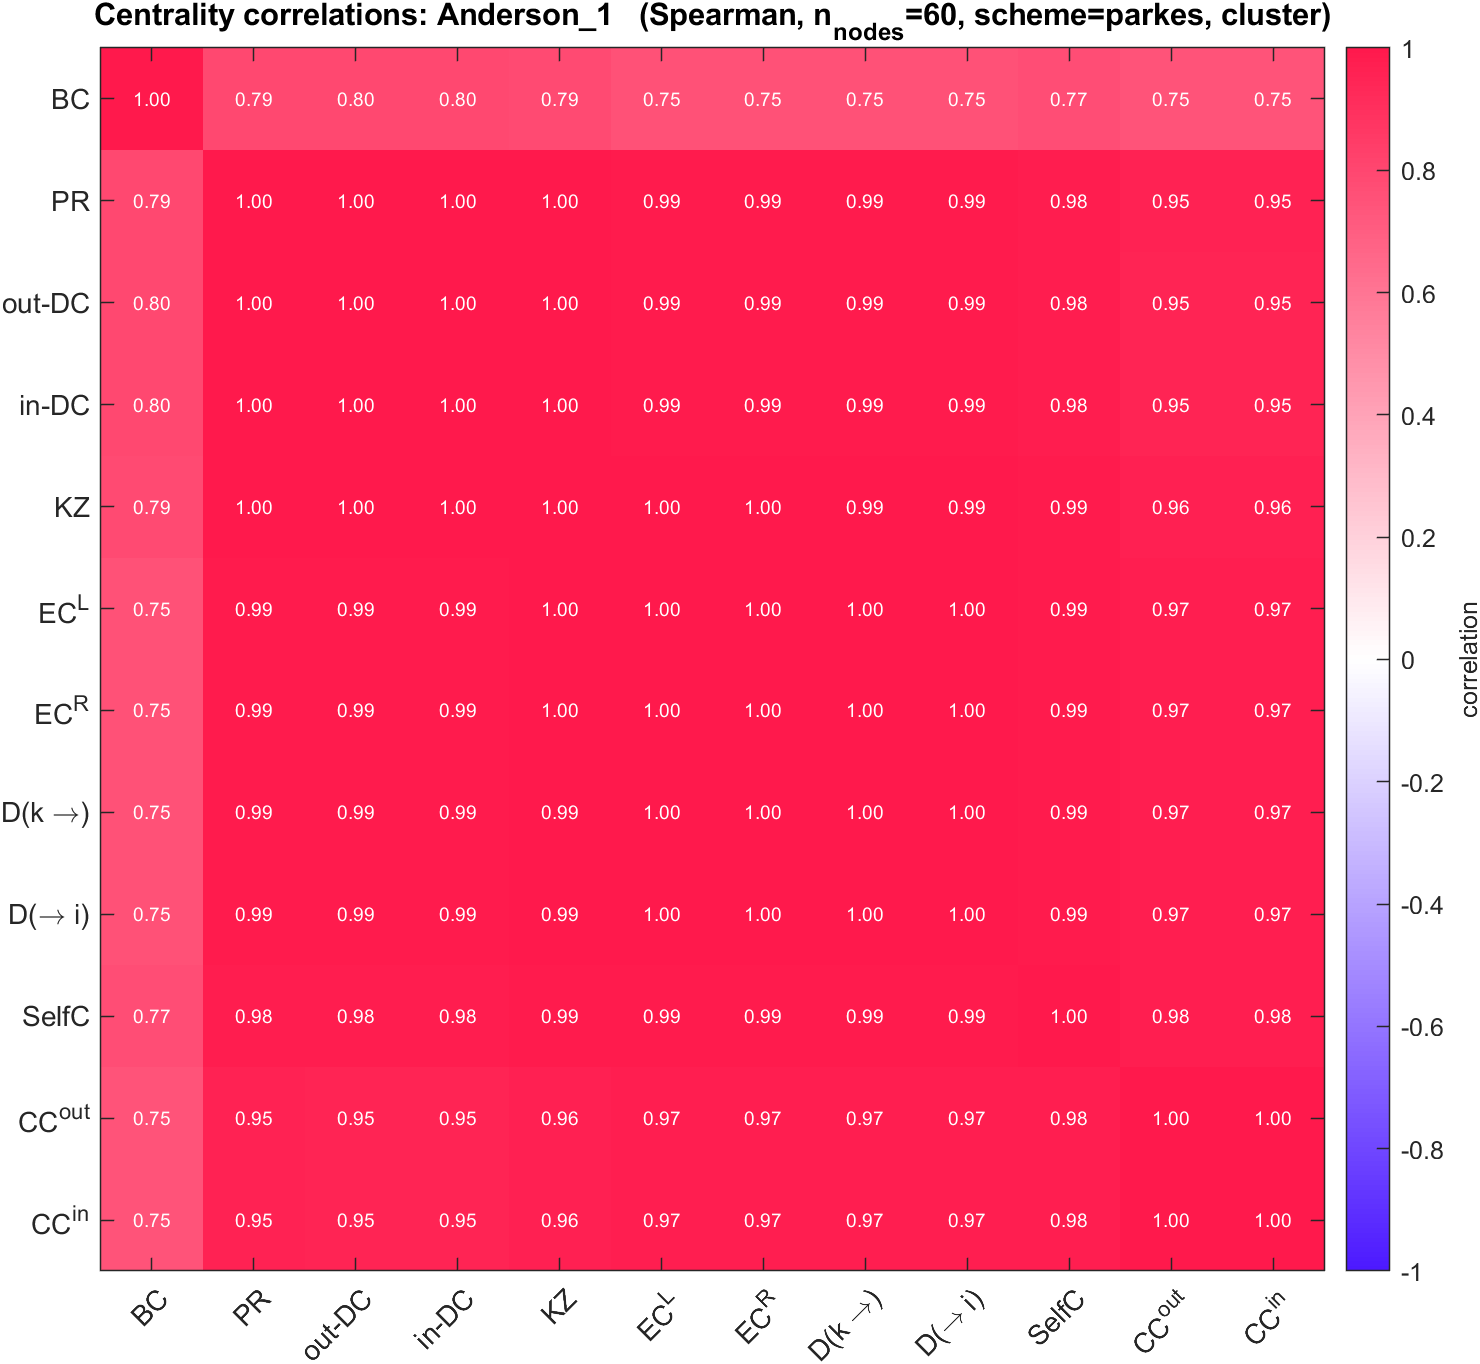
\includegraphics[width=\linewidth]{appendix/centrality_corr_Anderson_1_parkes.png}
\caption{\textsc{Anderson\_1}}
\end{subfigure}\hfill
\begin{subfigure}{0.32\textwidth}\centering
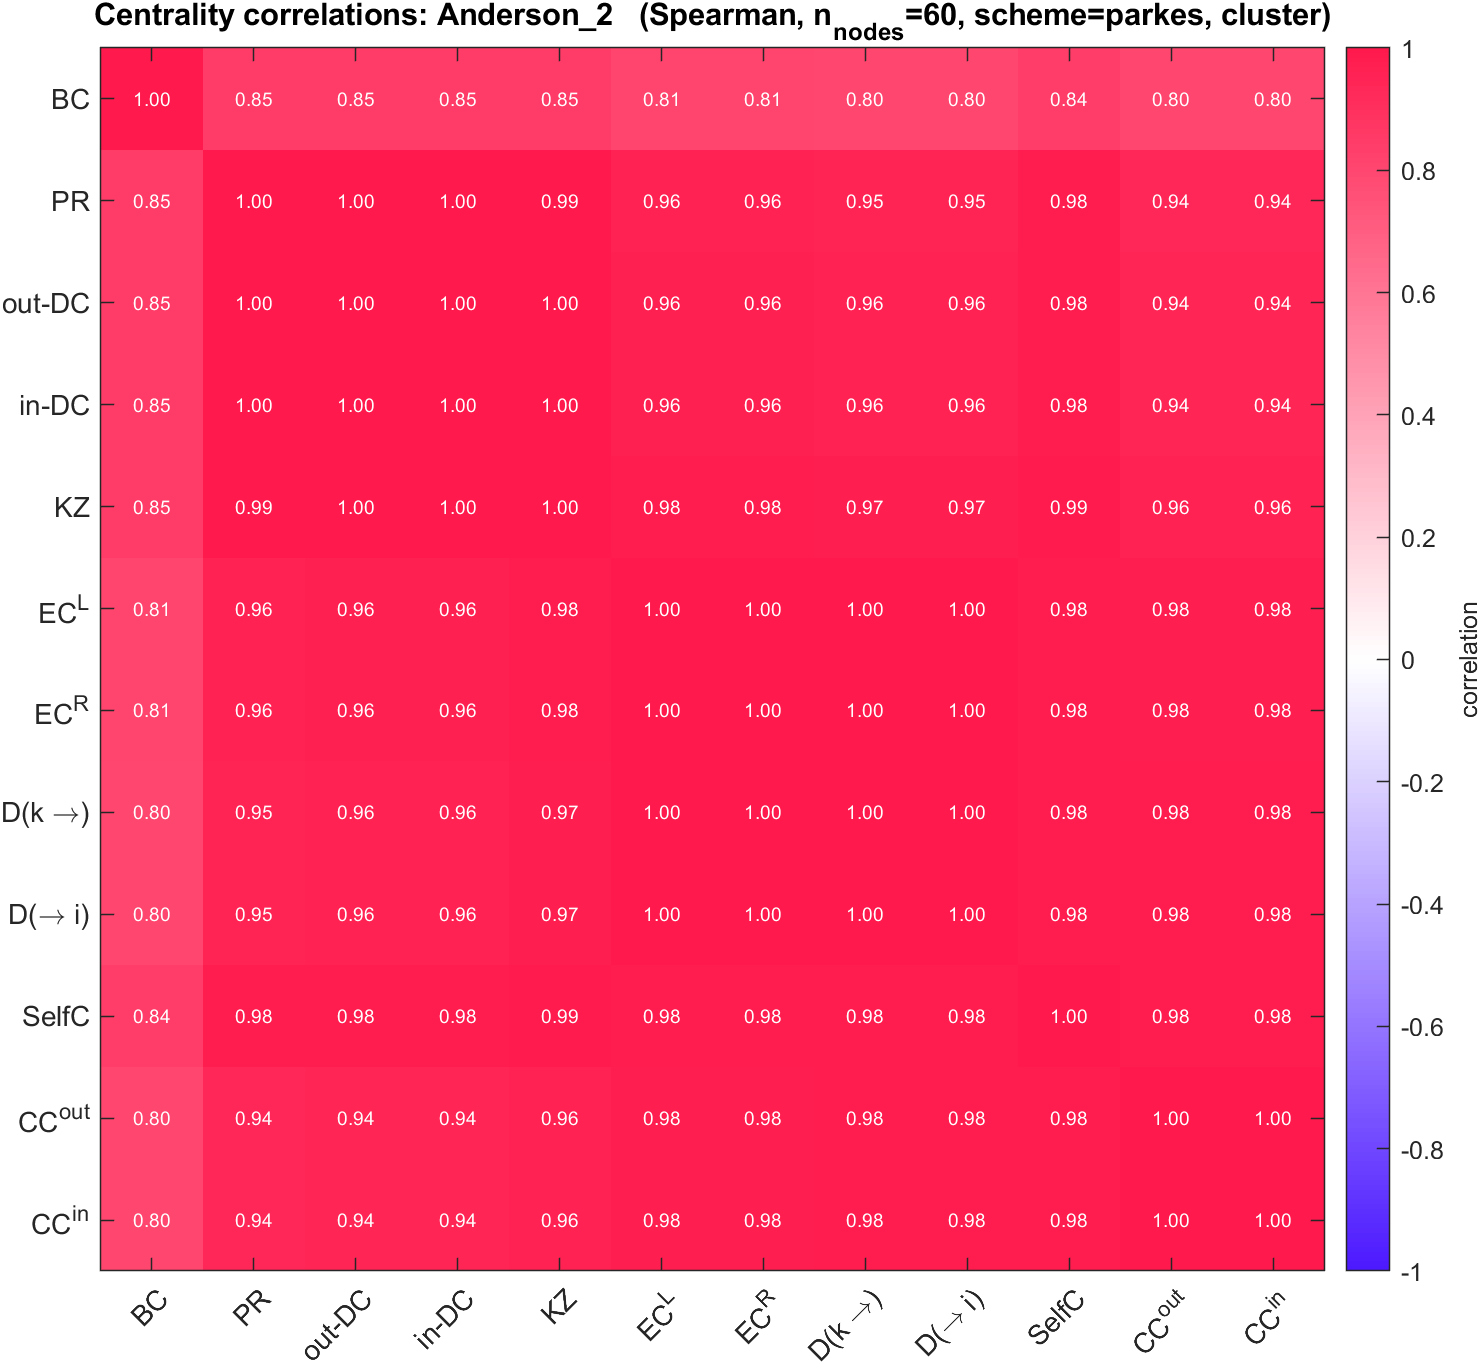
\includegraphics[width=\linewidth]{appendix/centrality_corr_Anderson_2_parkes.png}
\caption{\textsc{Anderson\_2}}
\end{subfigure}\hfill
\begin{subfigure}{0.32\textwidth}\centering
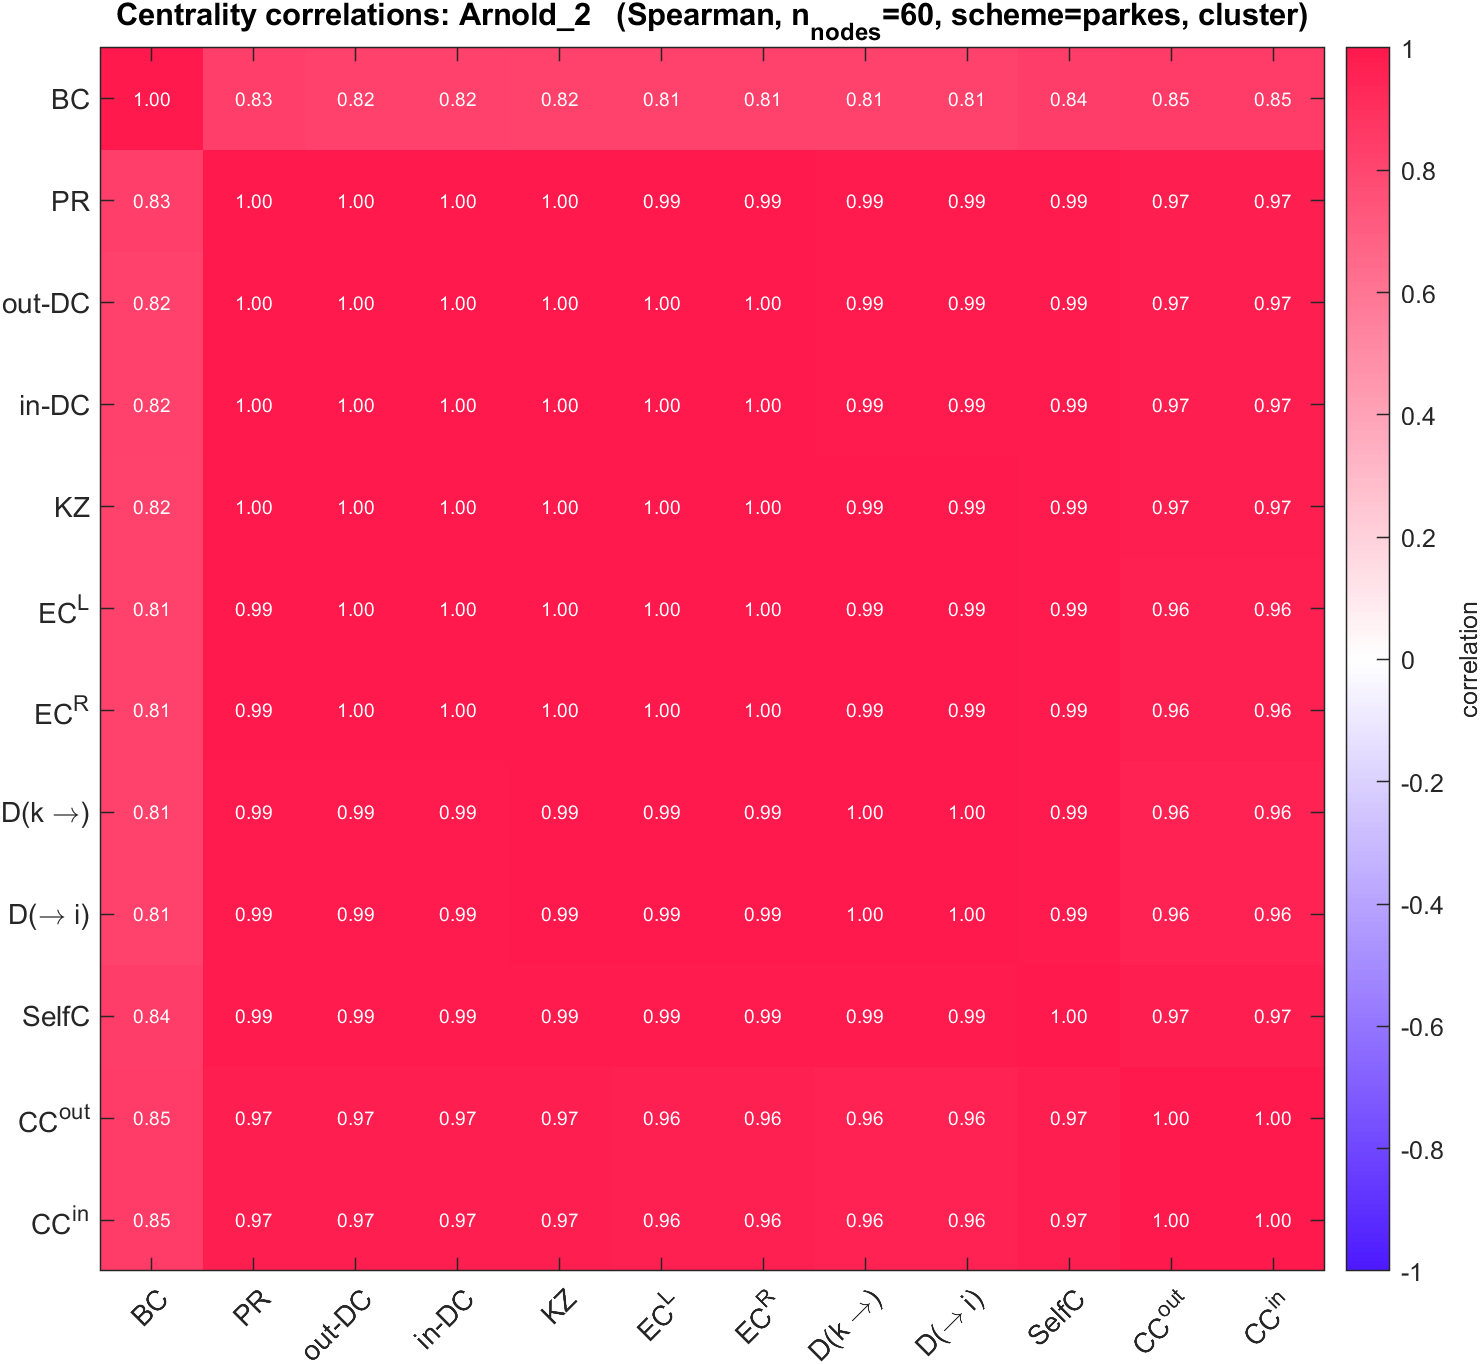
\includegraphics[width=\linewidth]{appendix/centrality_corr_Arnold_2_parkes.png}
\caption{\textsc{Arnold\_2}}
\end{subfigure}\hfill
\begin{subfigure}{0.32\textwidth}\centering
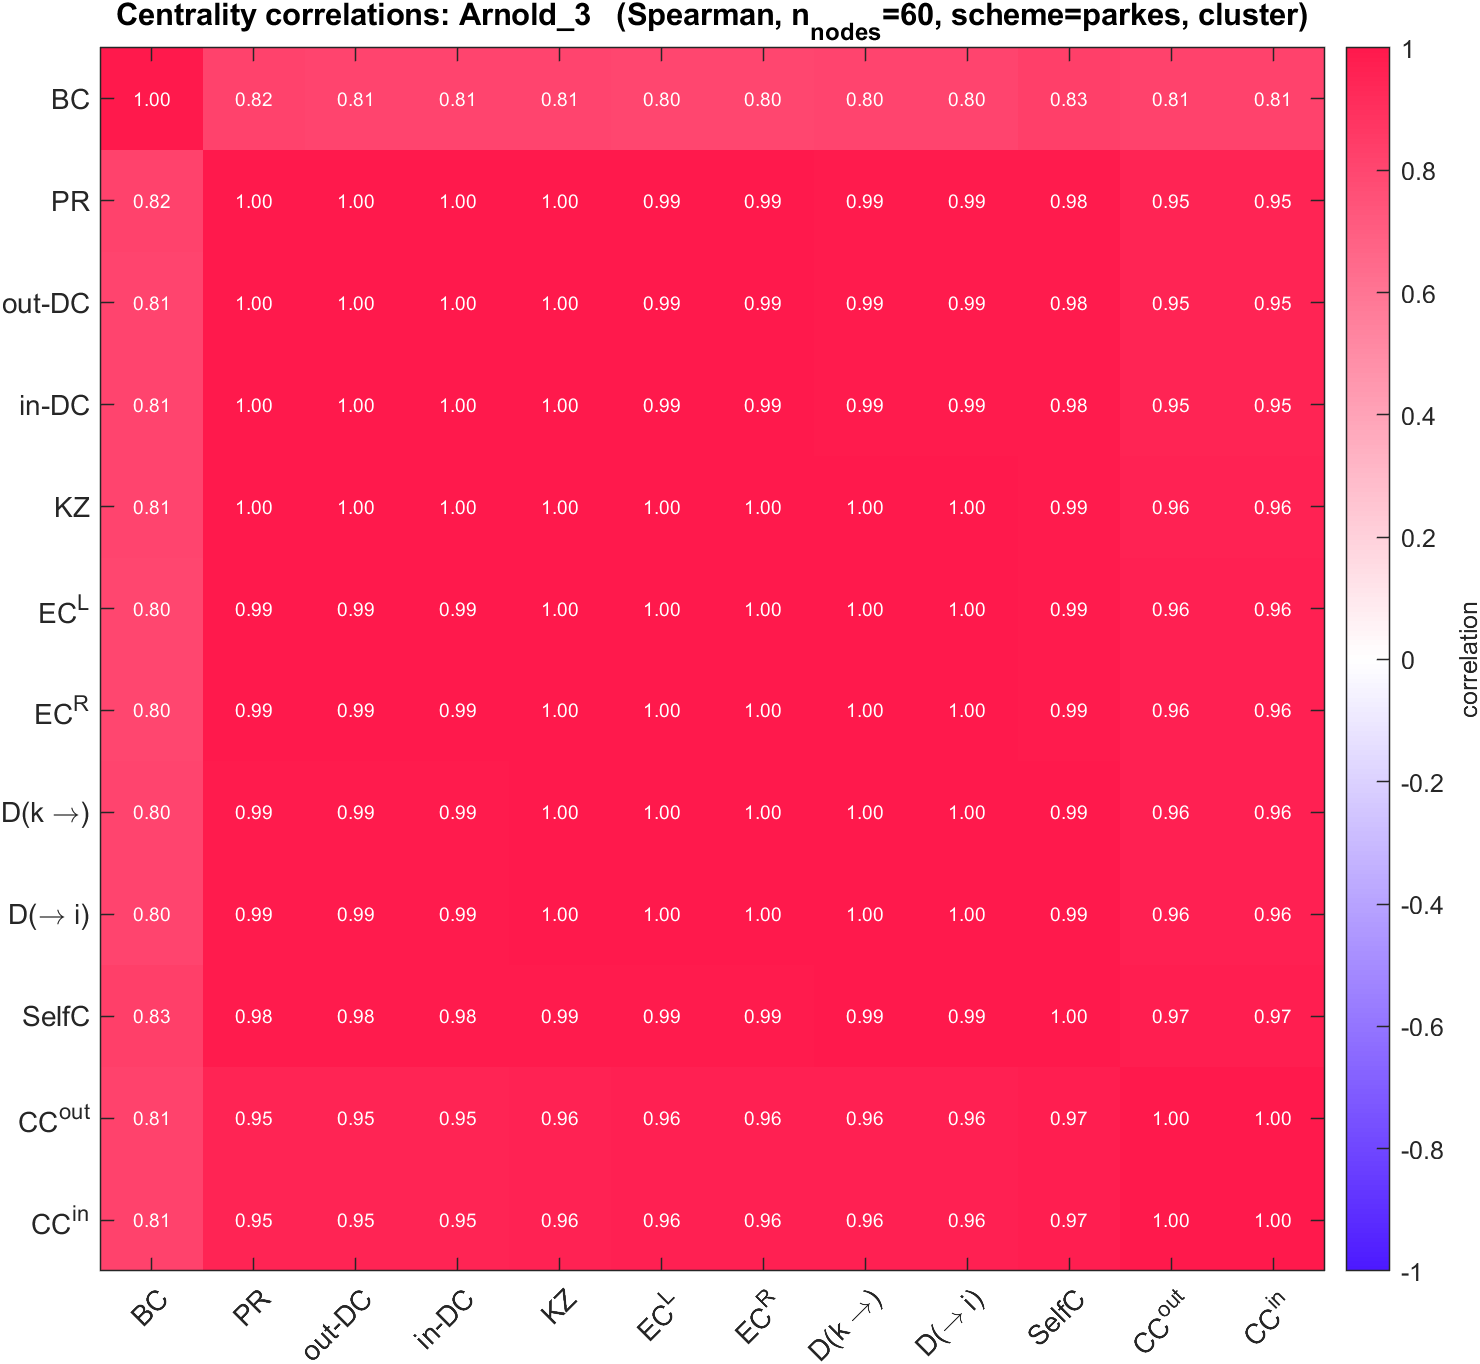
\includegraphics[width=\linewidth]{appendix/centrality_corr_Arnold_3_parkes.png}
\caption{\textsc{Arnold\_3}}
\end{subfigure}\hfill
\begin{subfigure}{0.32\textwidth}\centering
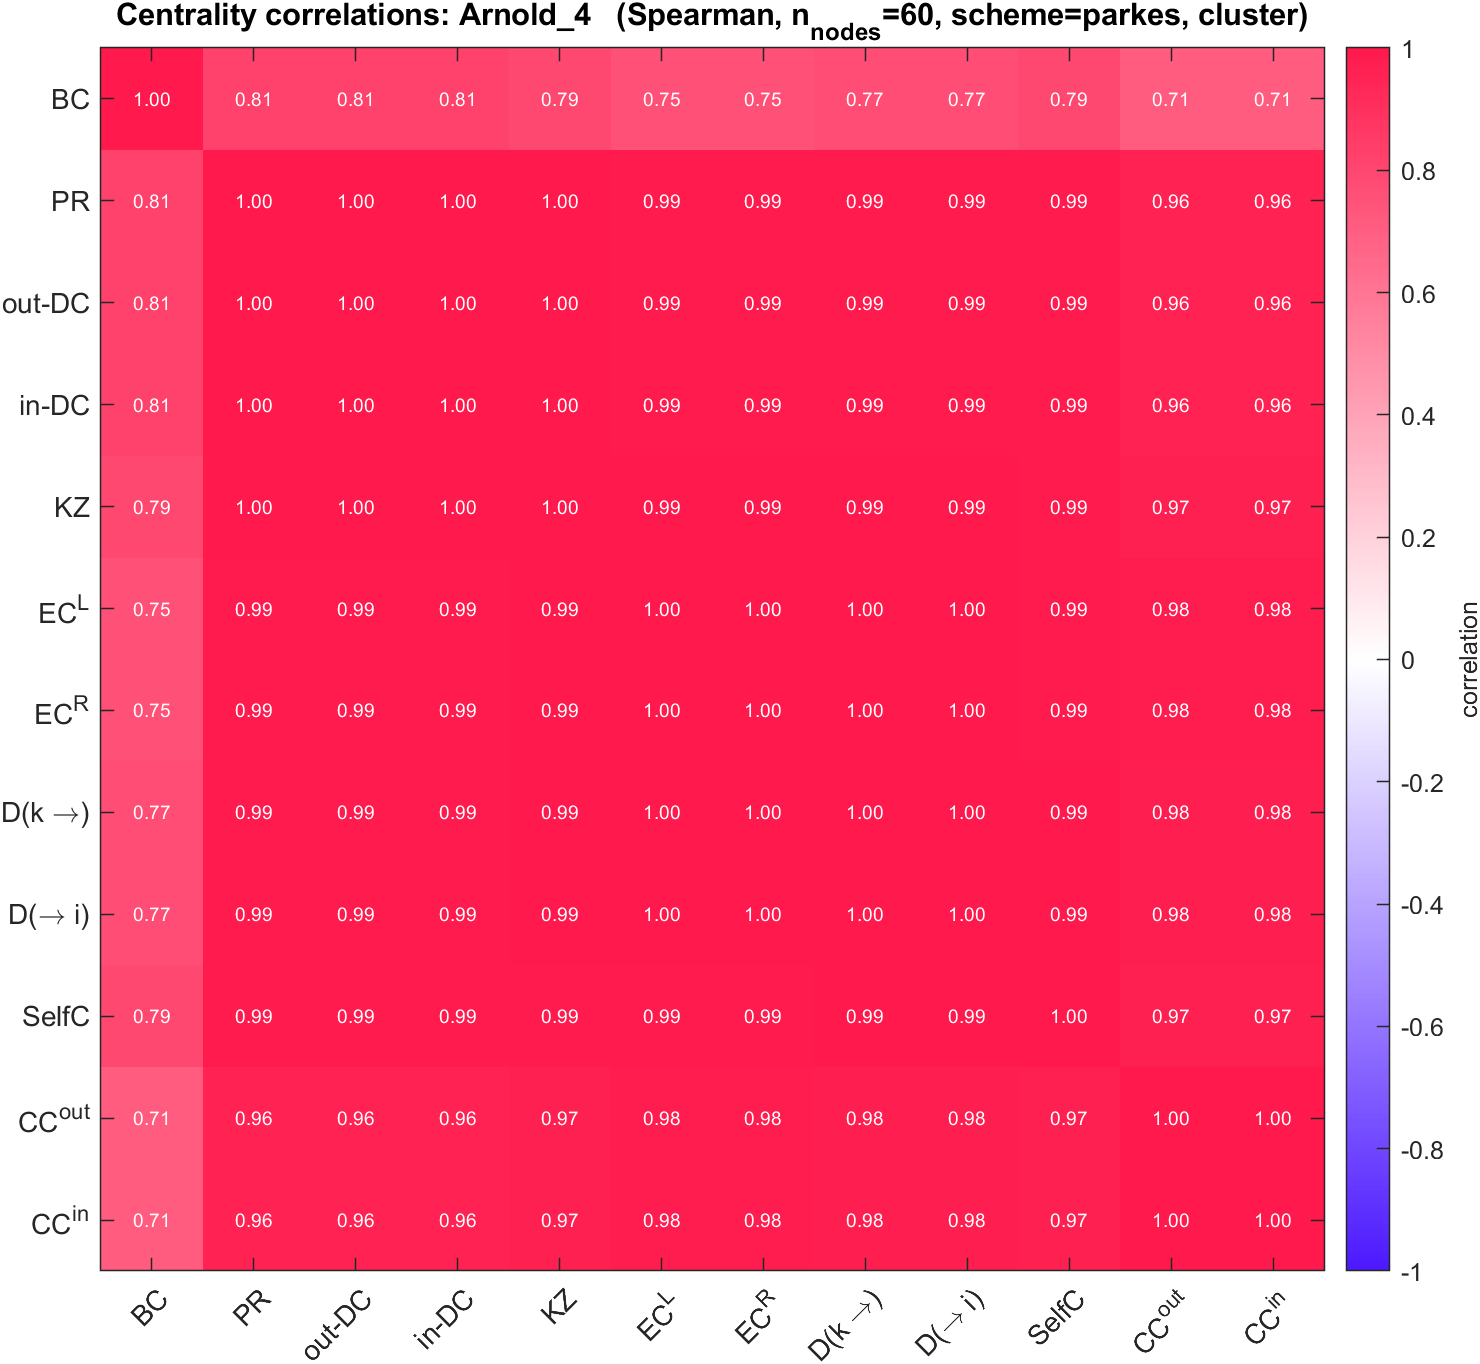
\includegraphics[width=\linewidth]{appendix/centrality_corr_Arnold_4_parkes.png}
\caption{\textsc{Arnold\_4}}
\end{subfigure}\hfill
\begin{subfigure}{0.32\textwidth}\centering
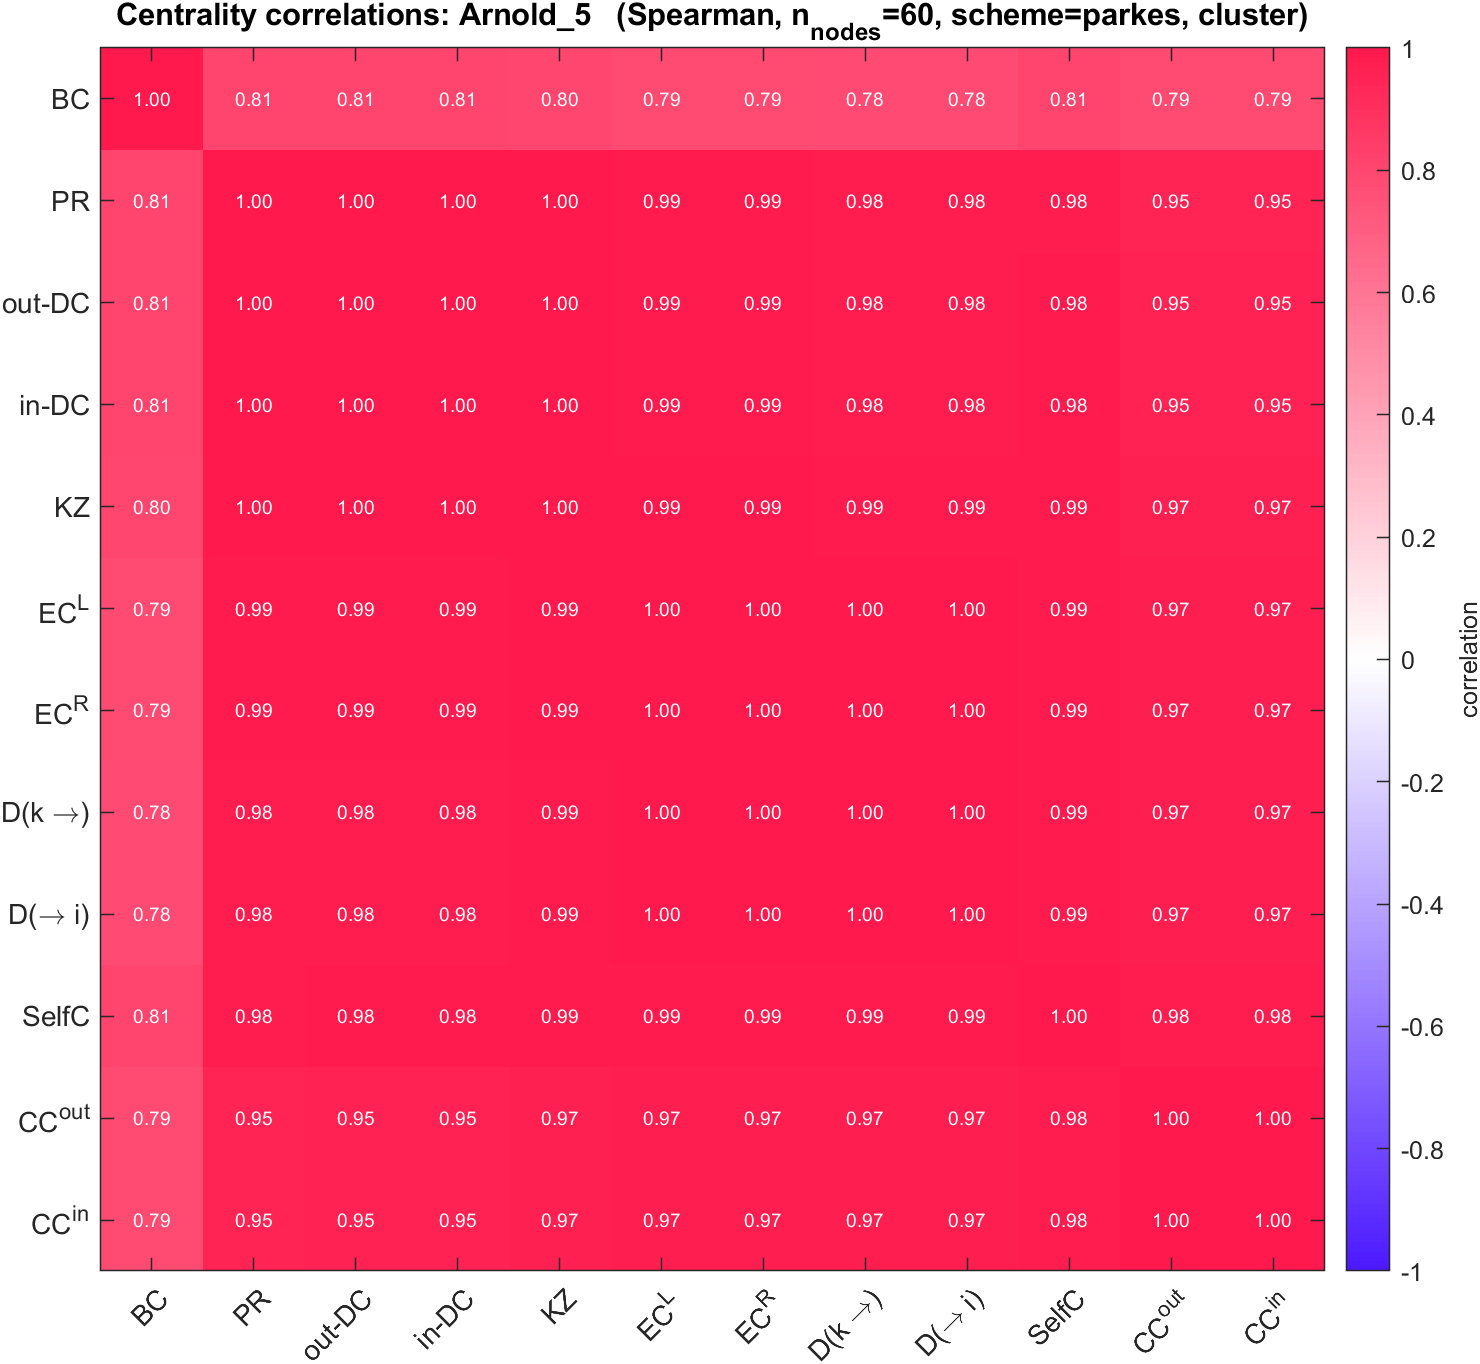
\includegraphics[width=\linewidth]{appendix/centrality_corr_Arnold_5_parkes.png}
\caption{\textsc{Arnold\_5}}
\end{subfigure}\hfill
\caption{Per-mouse centrality correlation matrices, \texttt{parkes} scheme.}
\end{figure}

\begin{figure}[H]\centering
\begin{subfigure}{0.48\textwidth}\centering
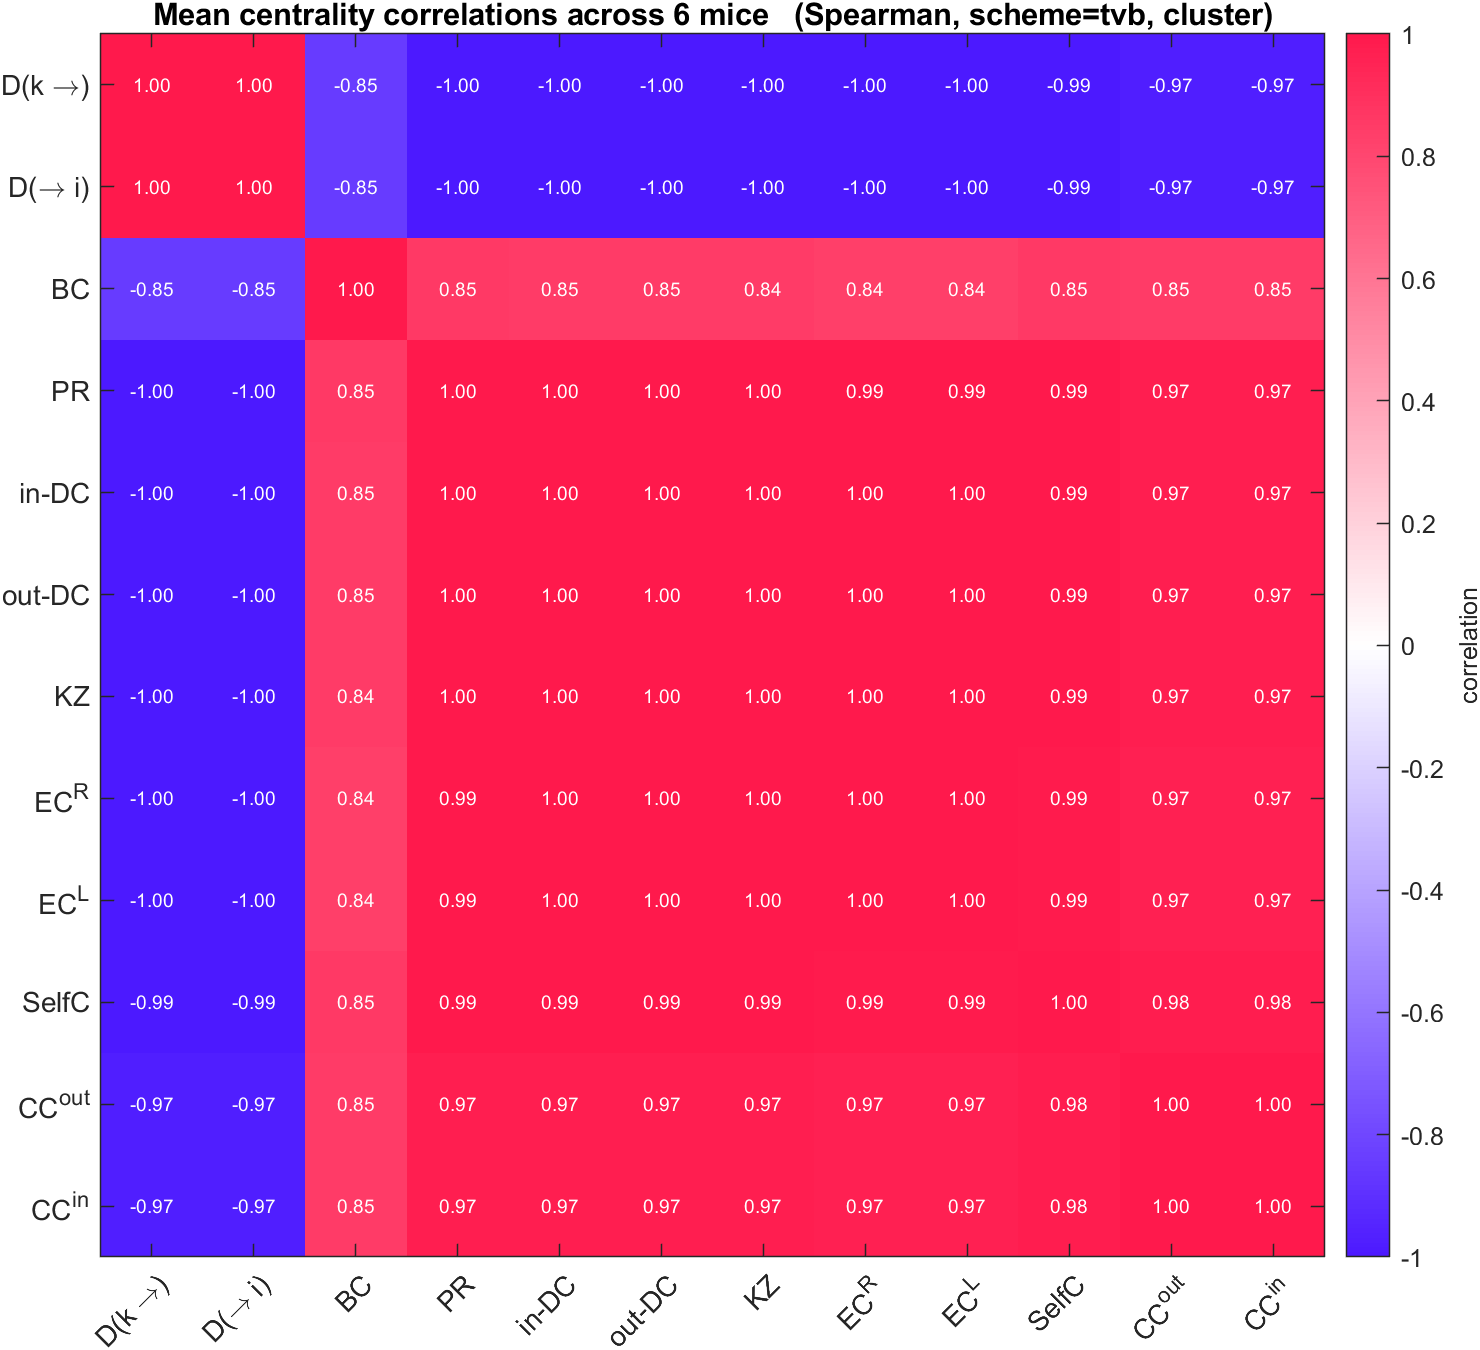
\includegraphics[width=\linewidth]{appendix/centrality_corr_mean_tvb.png}
\caption{Cohort mean}
\end{subfigure}\hfill
\begin{subfigure}{0.48\textwidth}\centering
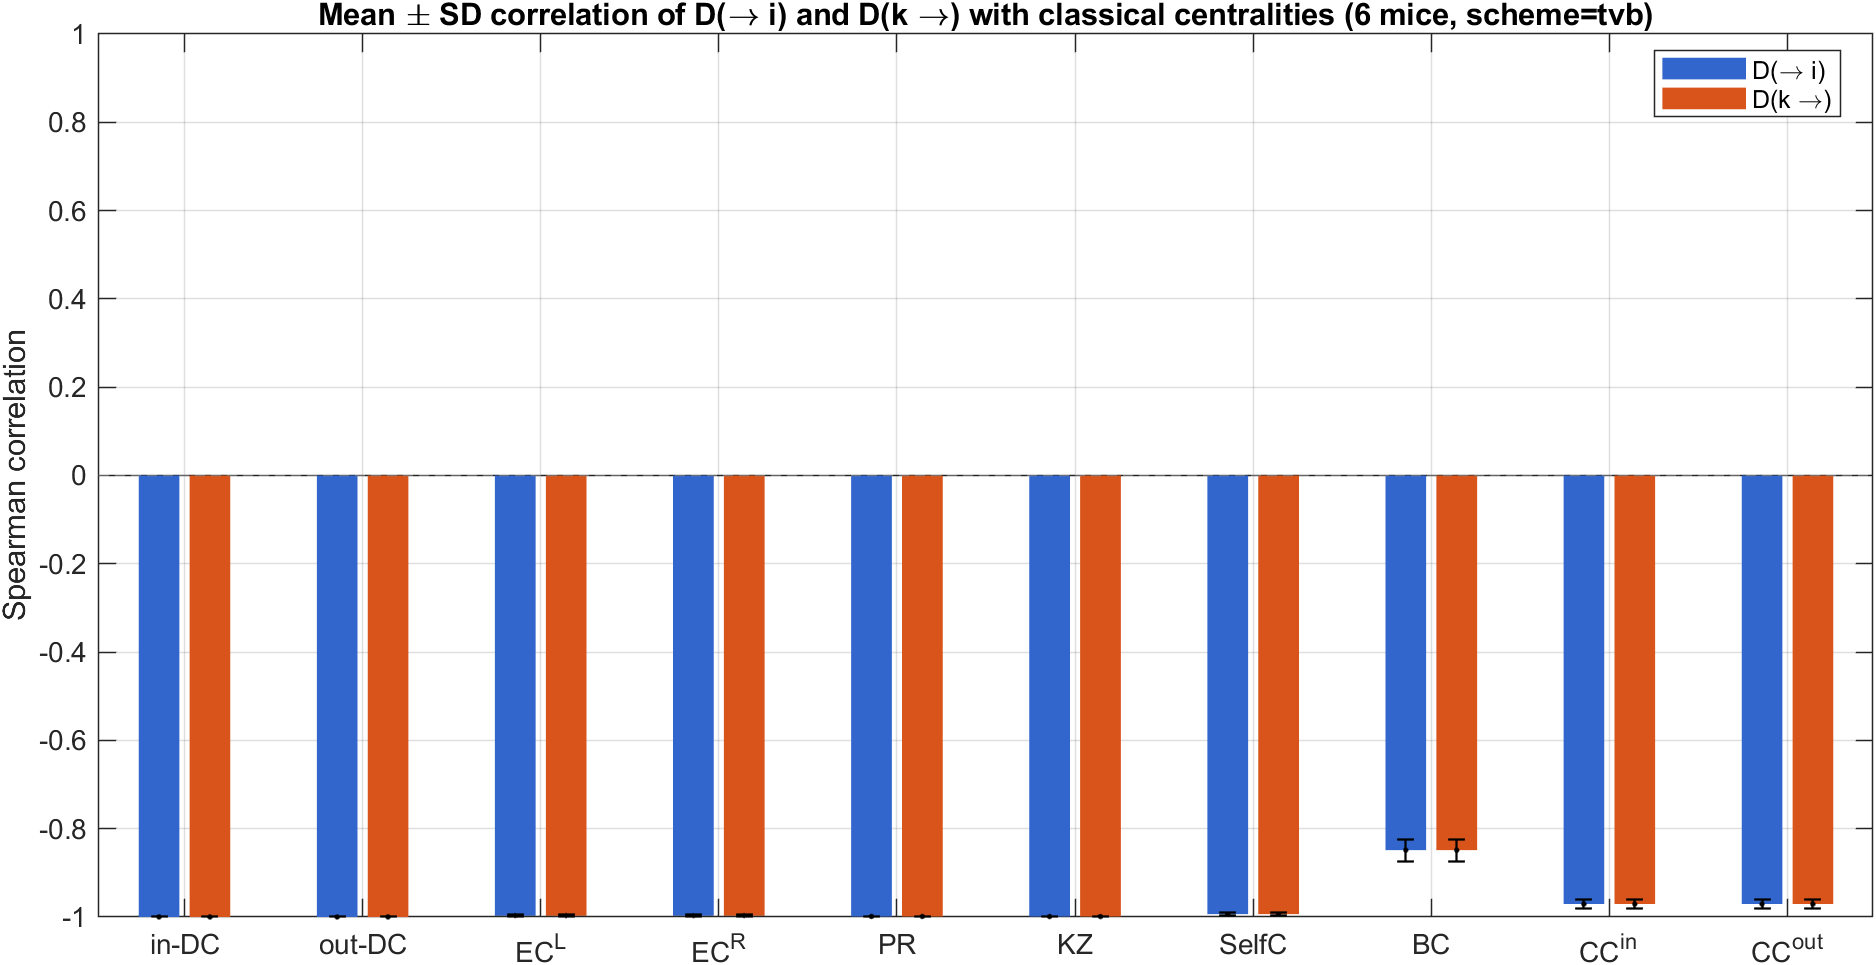
\includegraphics[width=\linewidth]{appendix/centrality_corr_bars_tvb.png}
\caption{$\Dto$, $\Dfrom$ vs classical}
\end{subfigure}
\caption{Centrality correlation summary, \texttt{tvb} scheme.}
\end{figure}
\begin{figure}[H]\centering
\begin{subfigure}{0.32\textwidth}\centering
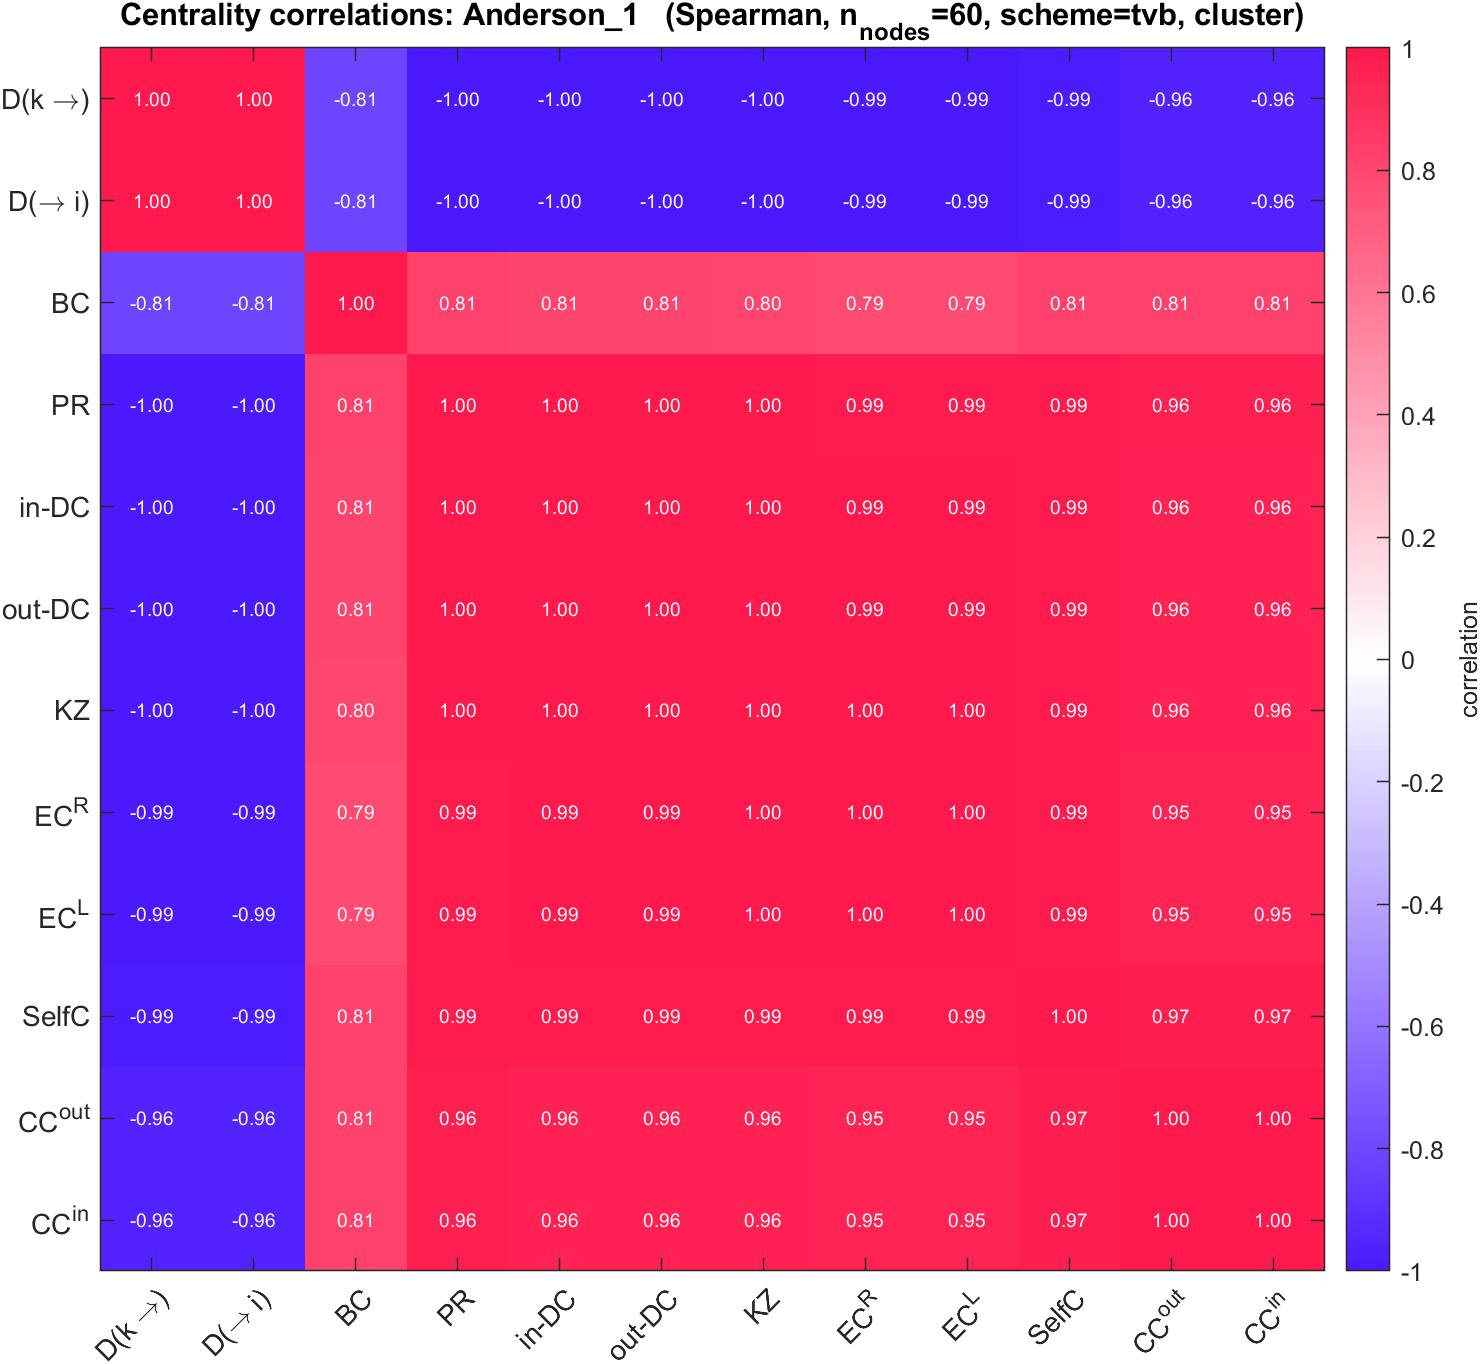
\includegraphics[width=\linewidth]{appendix/centrality_corr_Anderson_1_tvb.png}
\caption{\textsc{Anderson\_1}}
\end{subfigure}\hfill
\begin{subfigure}{0.32\textwidth}\centering
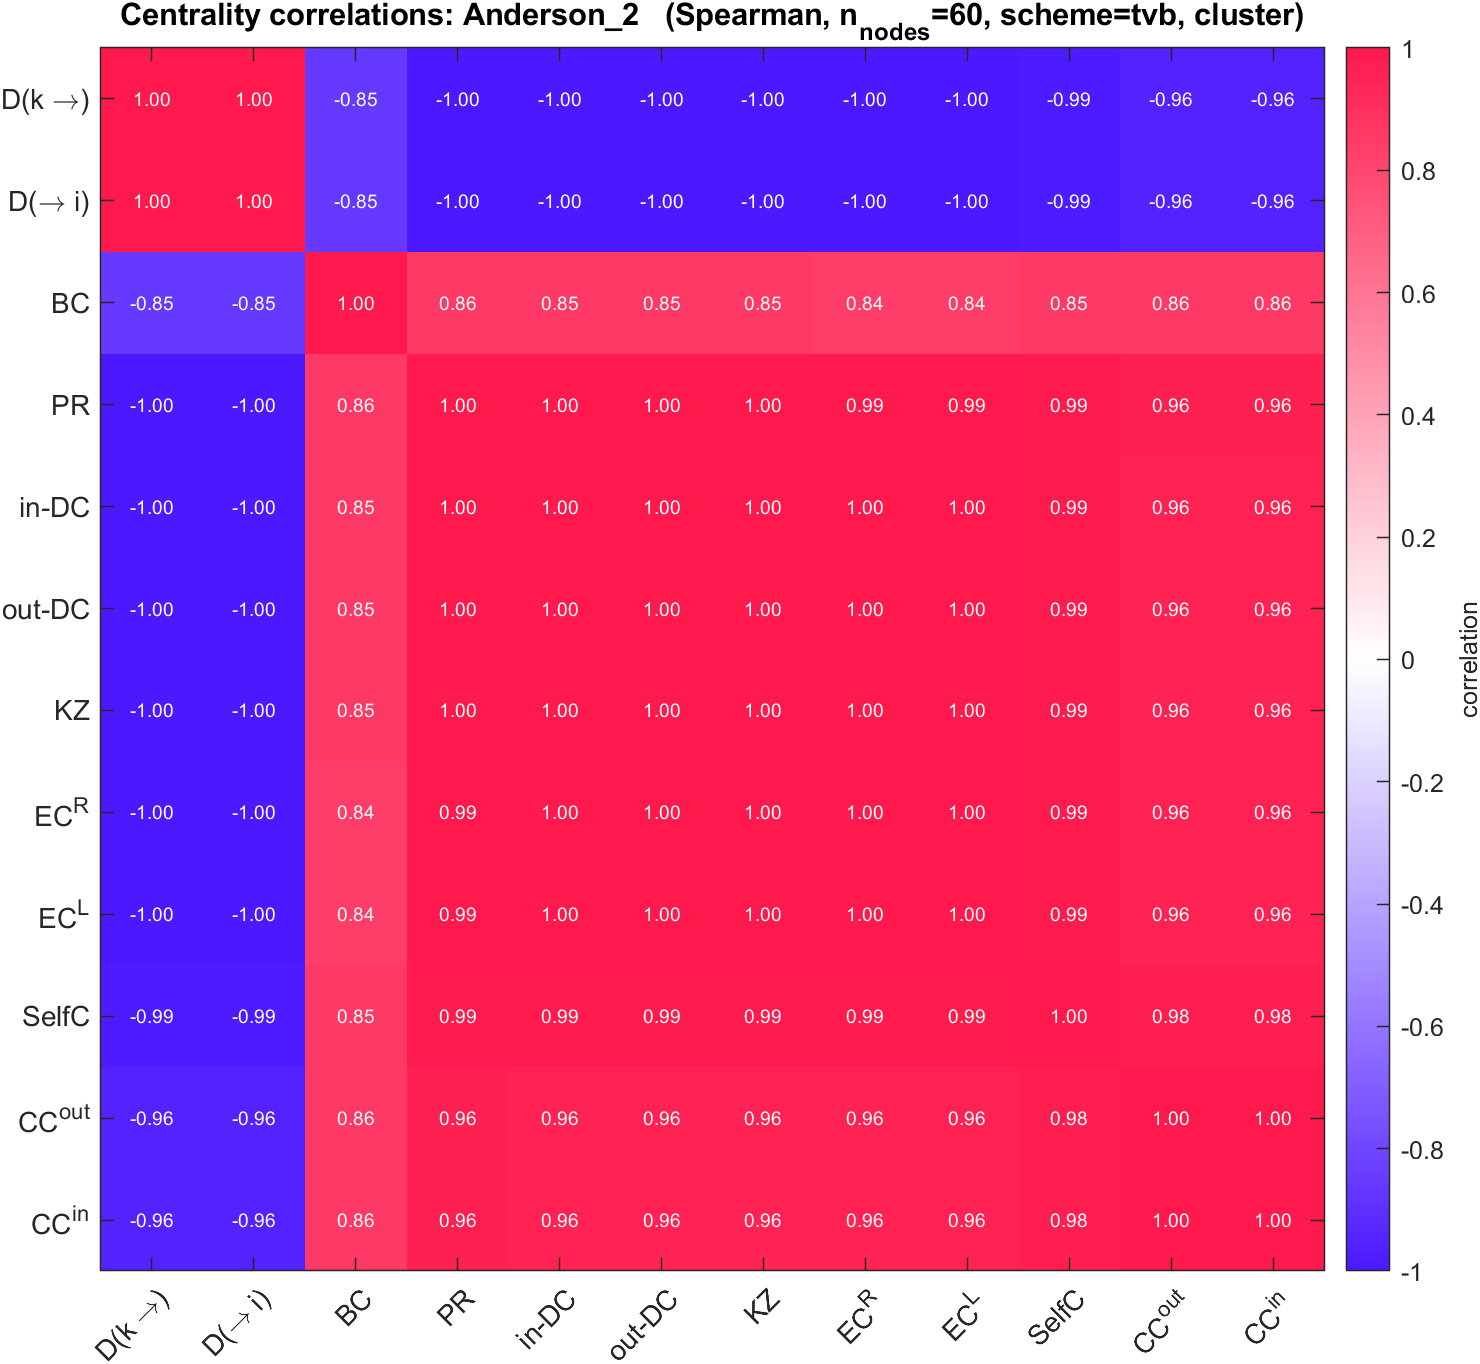
\includegraphics[width=\linewidth]{appendix/centrality_corr_Anderson_2_tvb.png}
\caption{\textsc{Anderson\_2}}
\end{subfigure}\hfill
\begin{subfigure}{0.32\textwidth}\centering
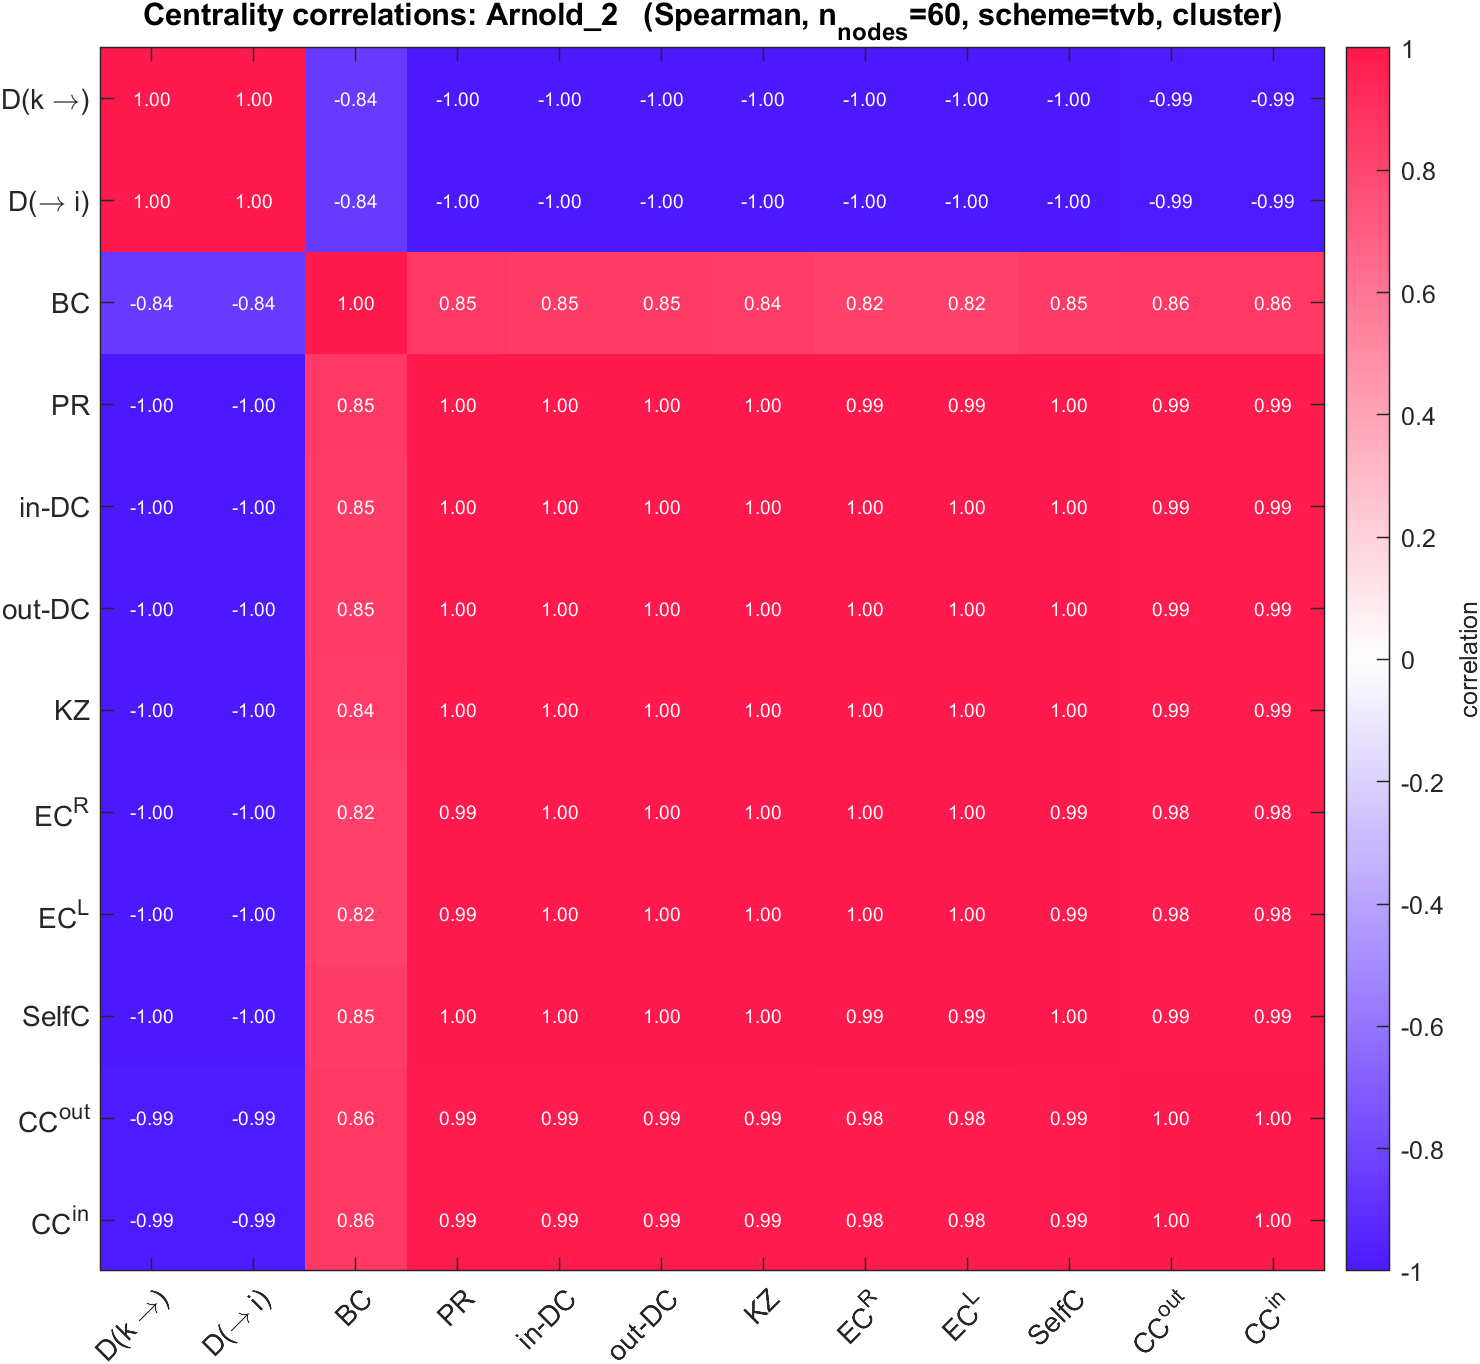
\includegraphics[width=\linewidth]{appendix/centrality_corr_Arnold_2_tvb.png}
\caption{\textsc{Arnold\_2}}
\end{subfigure}\hfill
\begin{subfigure}{0.32\textwidth}\centering
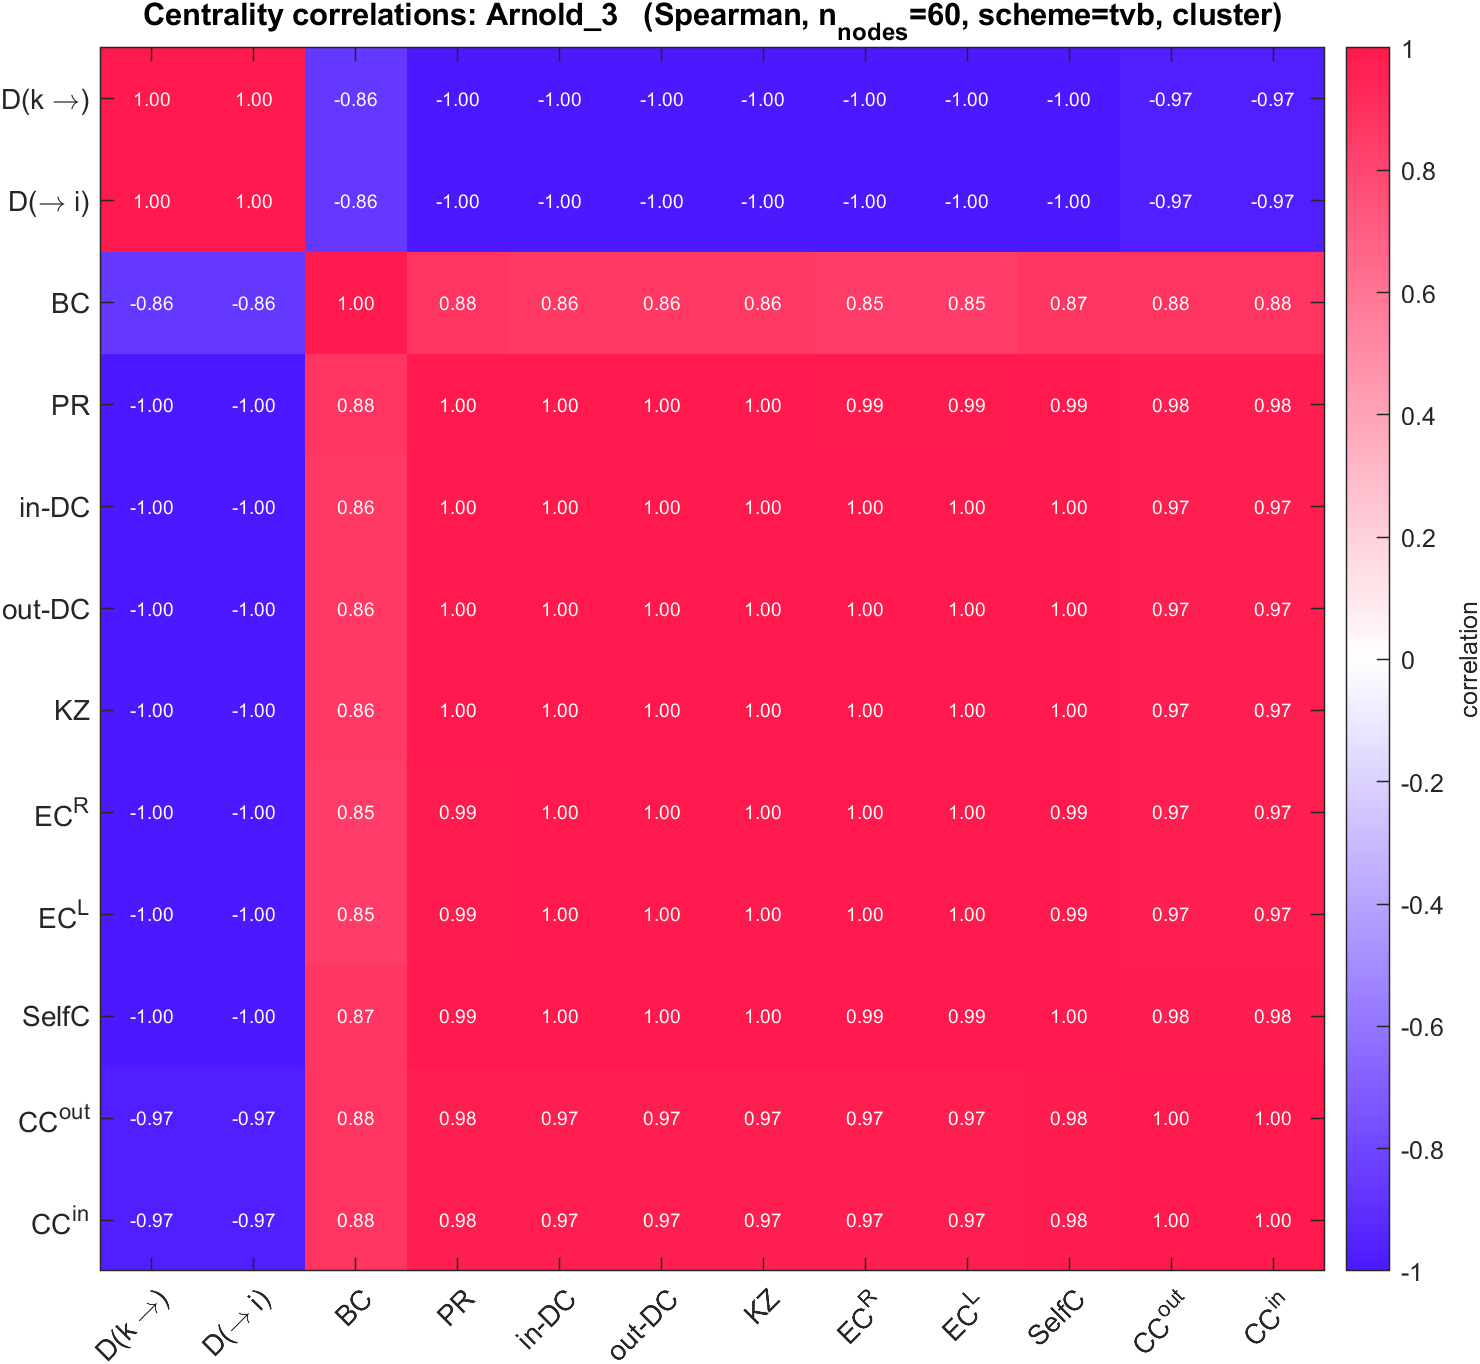
\includegraphics[width=\linewidth]{appendix/centrality_corr_Arnold_3_tvb.png}
\caption{\textsc{Arnold\_3}}
\end{subfigure}\hfill
\begin{subfigure}{0.32\textwidth}\centering
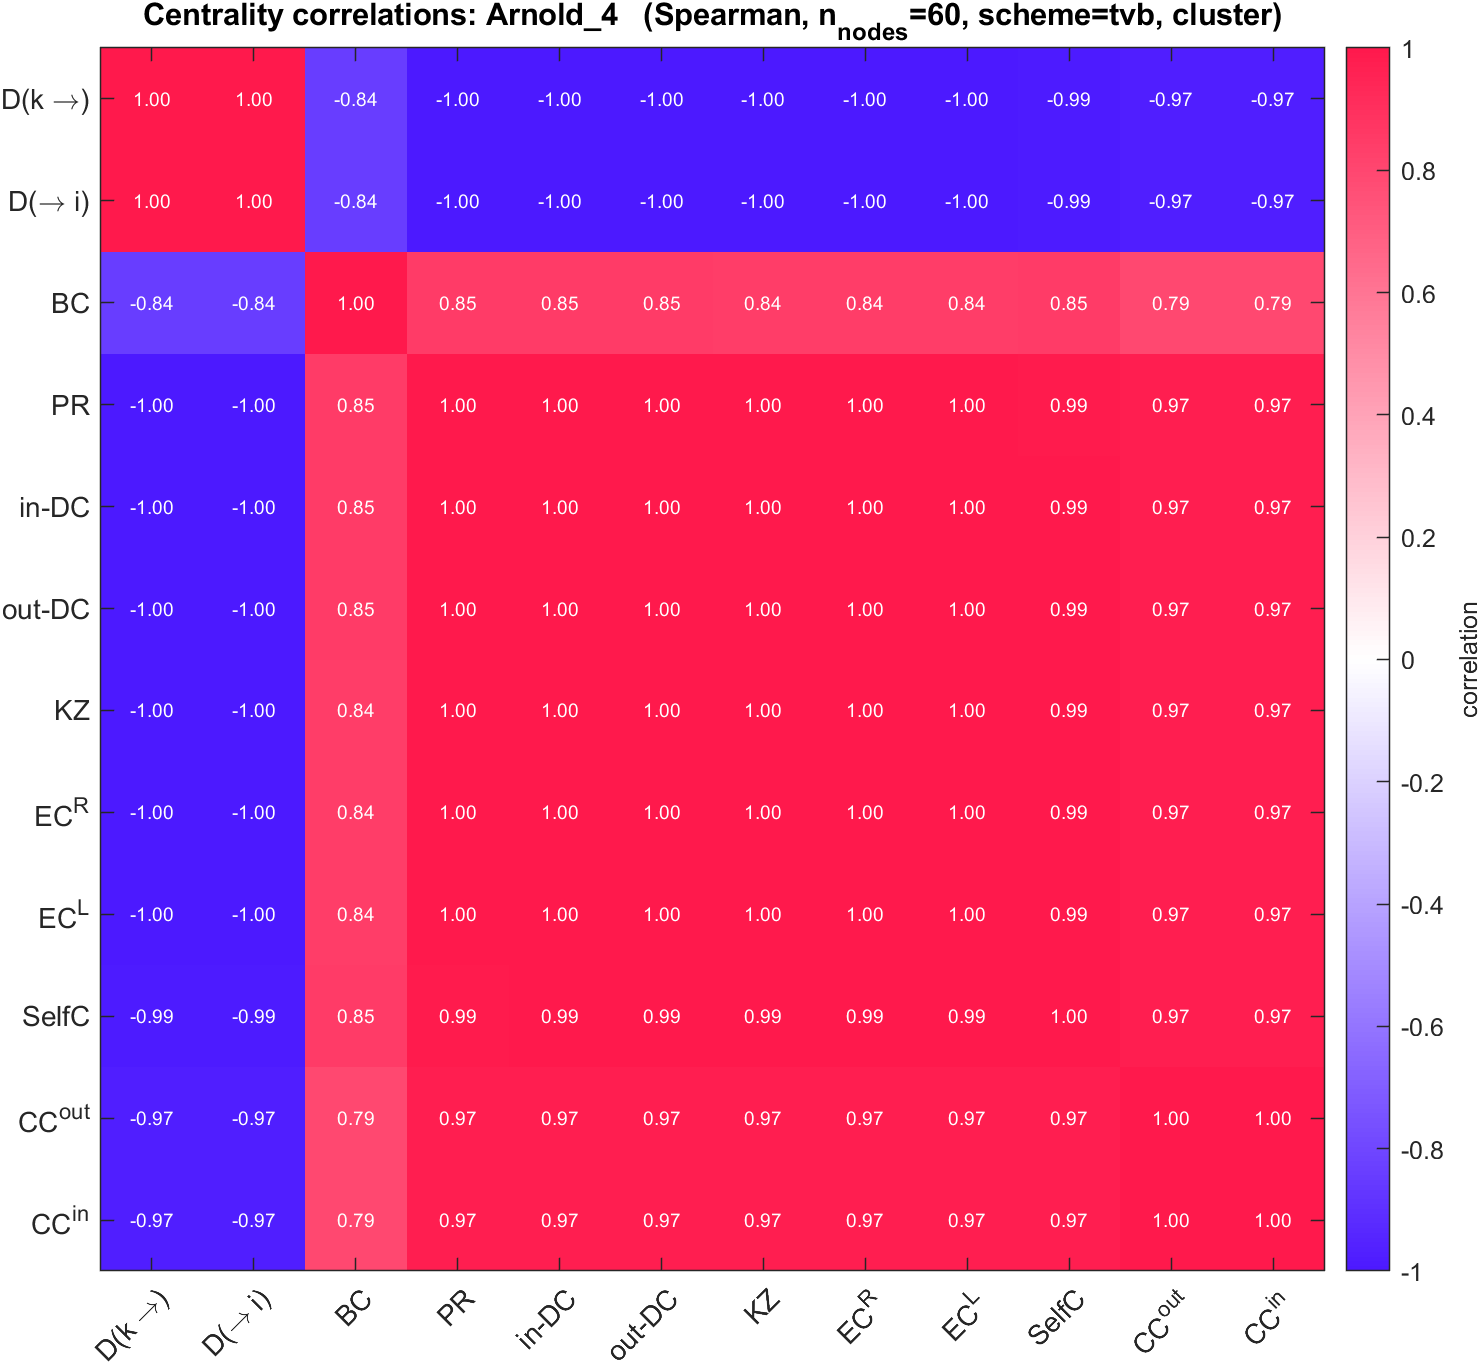
\includegraphics[width=\linewidth]{appendix/centrality_corr_Arnold_4_tvb.png}
\caption{\textsc{Arnold\_4}}
\end{subfigure}\hfill
\begin{subfigure}{0.32\textwidth}\centering
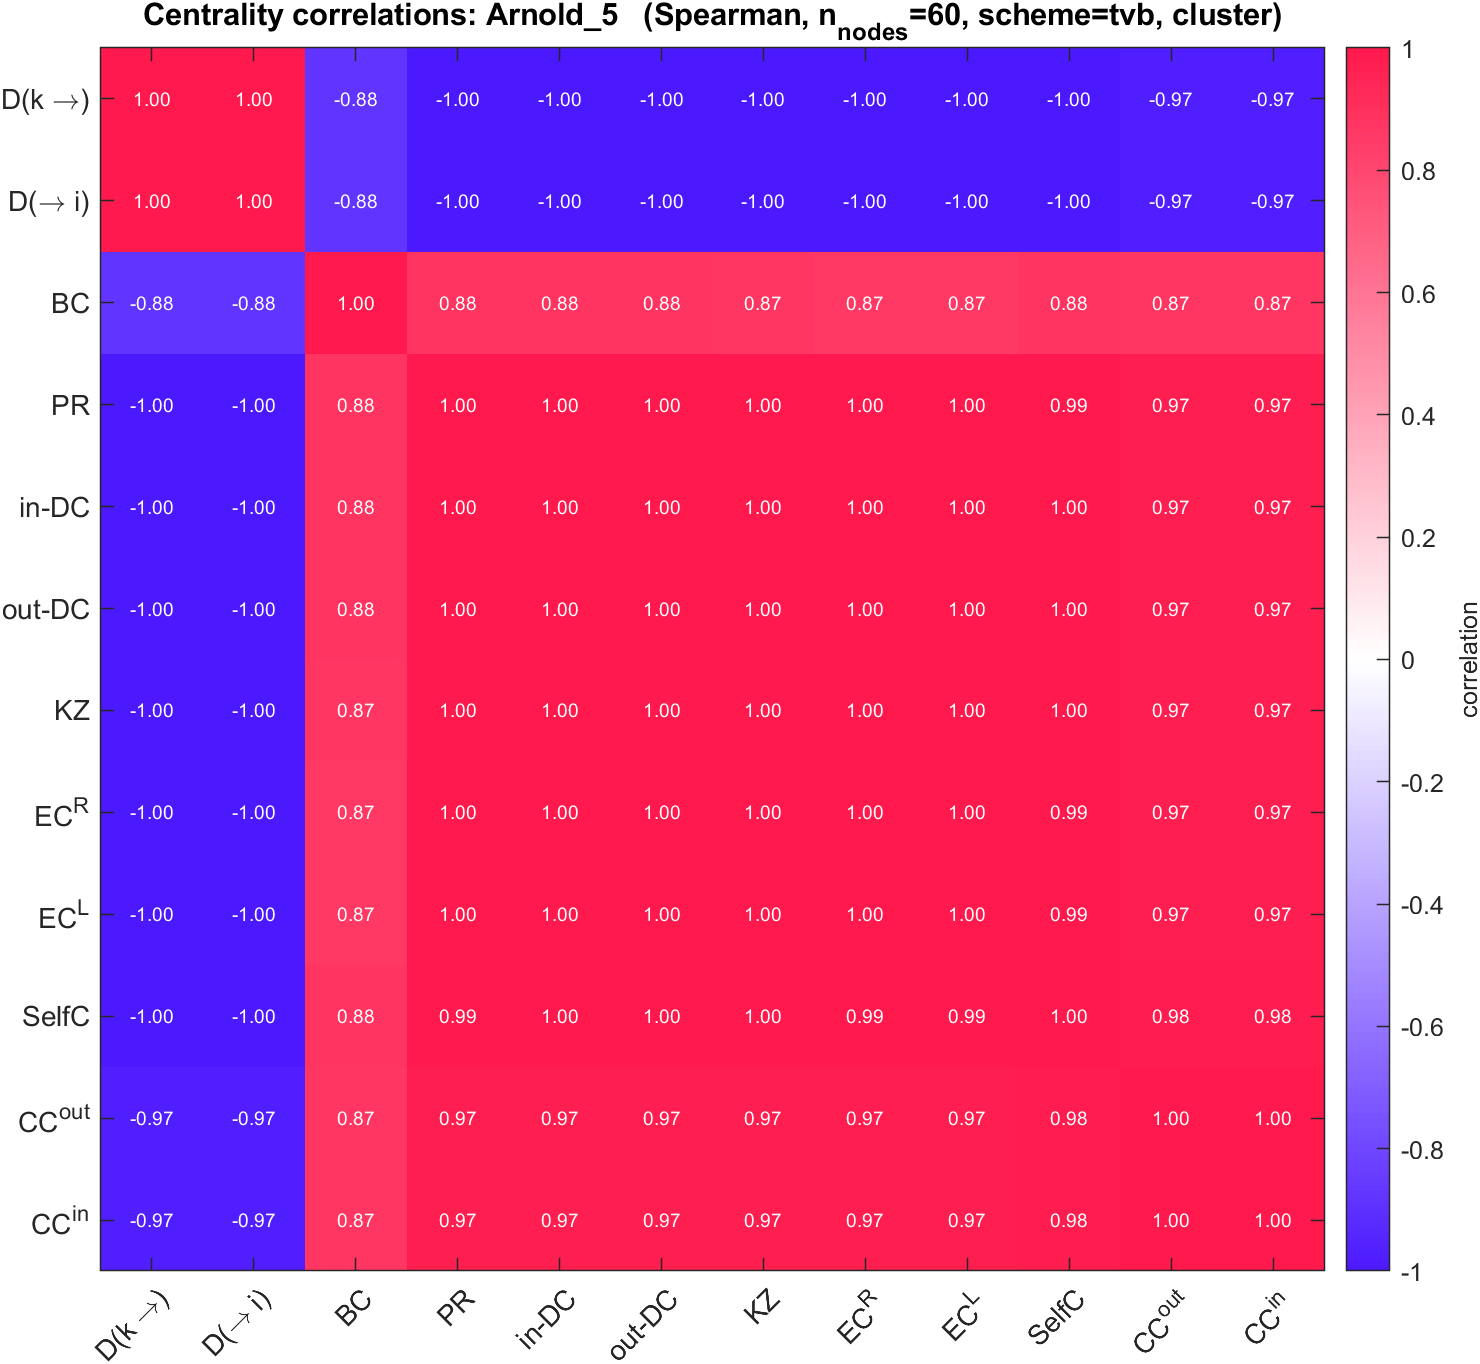
\includegraphics[width=\linewidth]{appendix/centrality_corr_Arnold_5_tvb.png}
\caption{\textsc{Arnold\_5}}
\end{subfigure}\hfill
\caption{Per-mouse centrality correlation matrices, \texttt{tvb} scheme.}
\end{figure}

\subsection{Anderson vs Arnold per-region contrasts}
\begin{figure}[H]\centering
\begin{subfigure}{0.32\textwidth}\centering
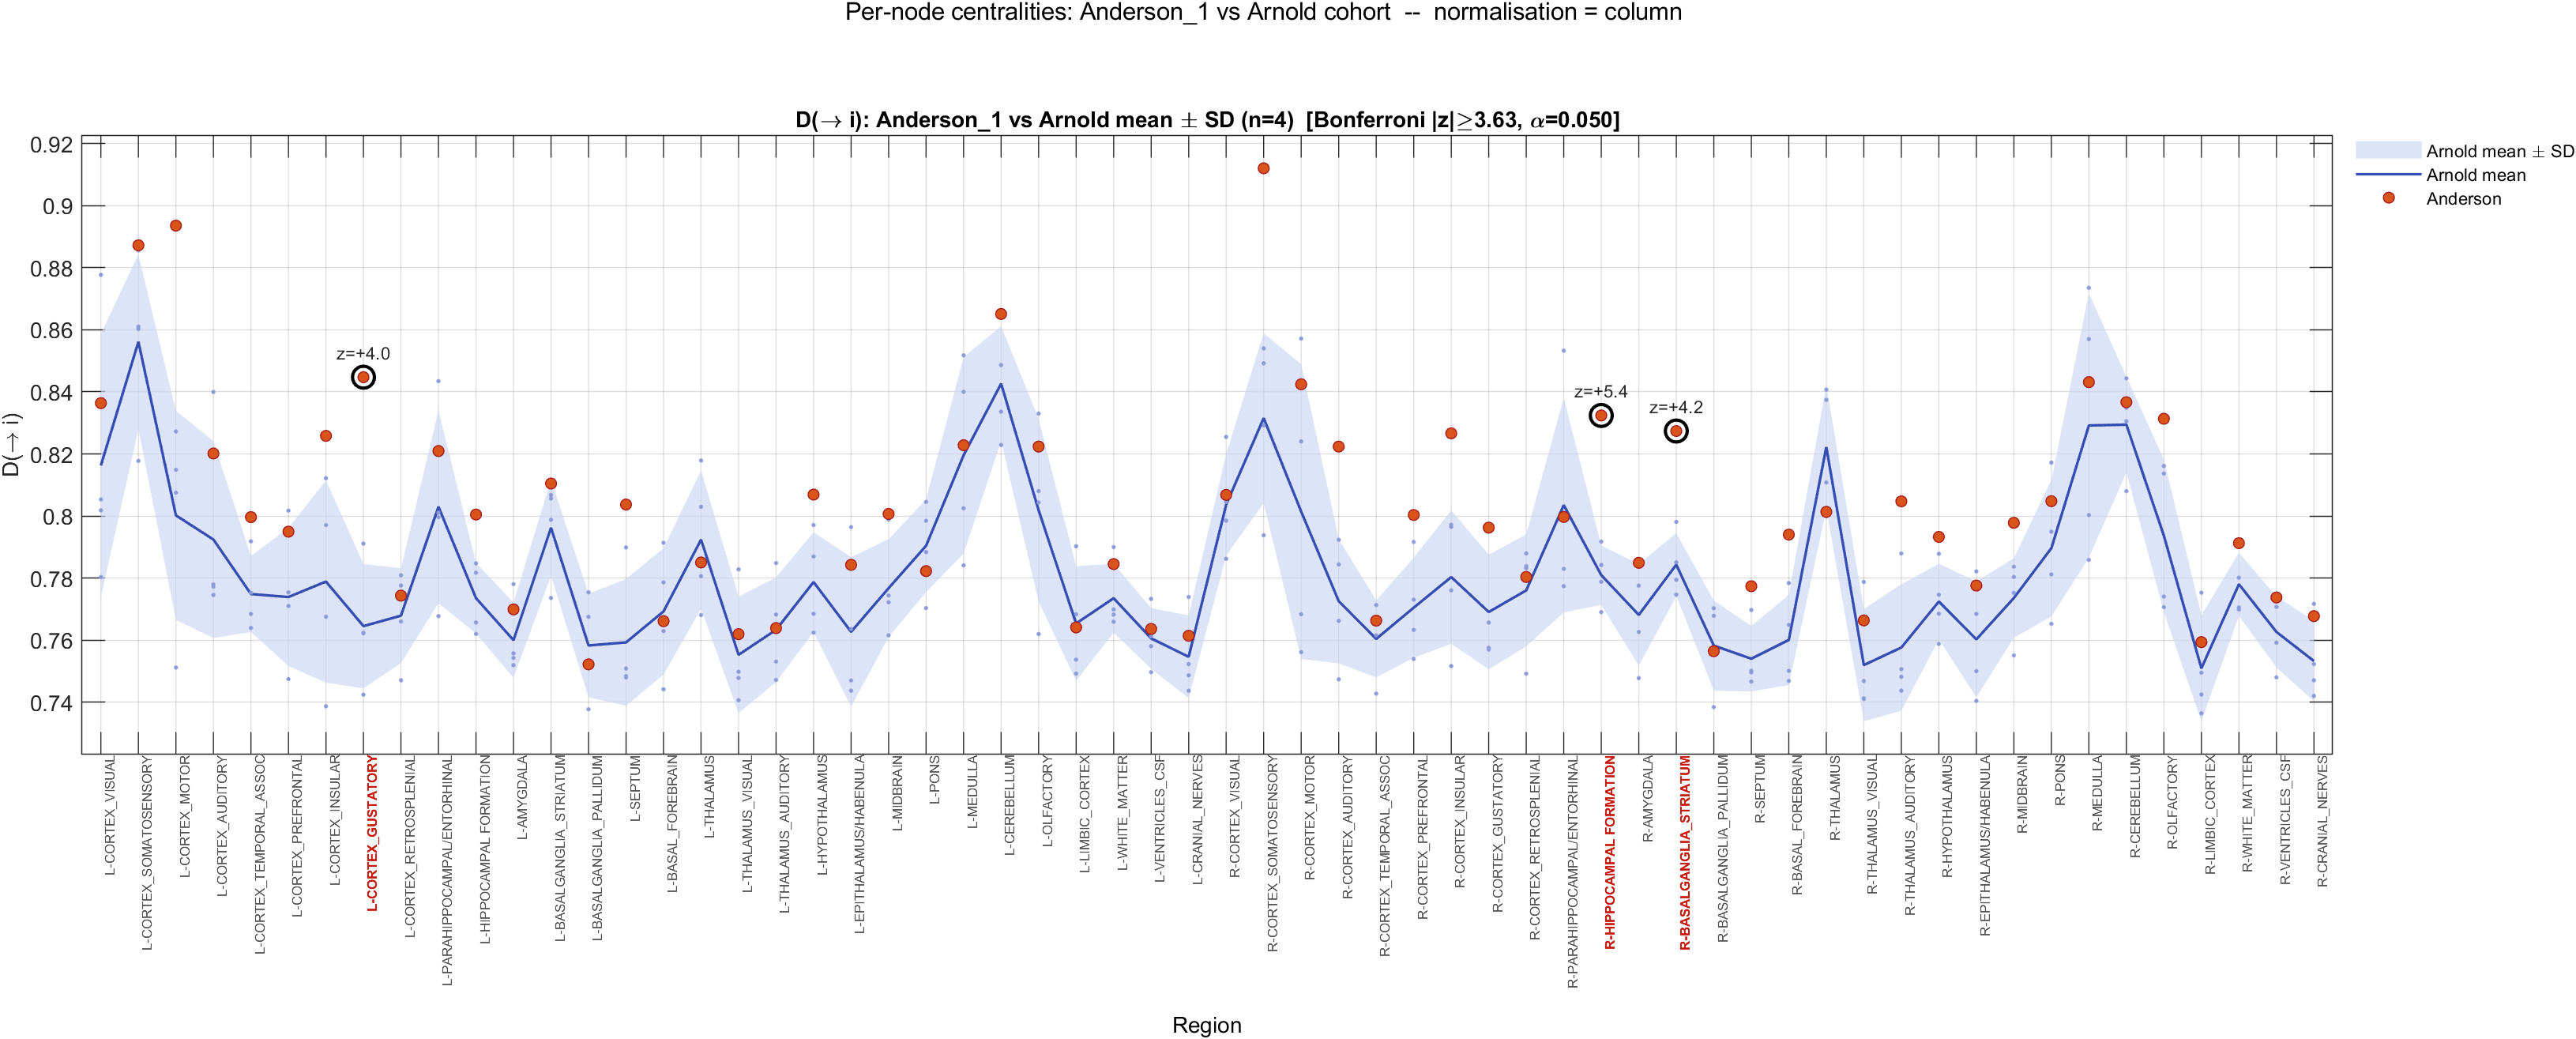
\includegraphics[width=\linewidth]{appendix/compare_anderson_vs_arnold_Anderson_1_column_D_to_i.png}
\caption{\textsc{Anderson\_1}, $\Dto$}
\end{subfigure}\hfill
\begin{subfigure}{0.32\textwidth}\centering
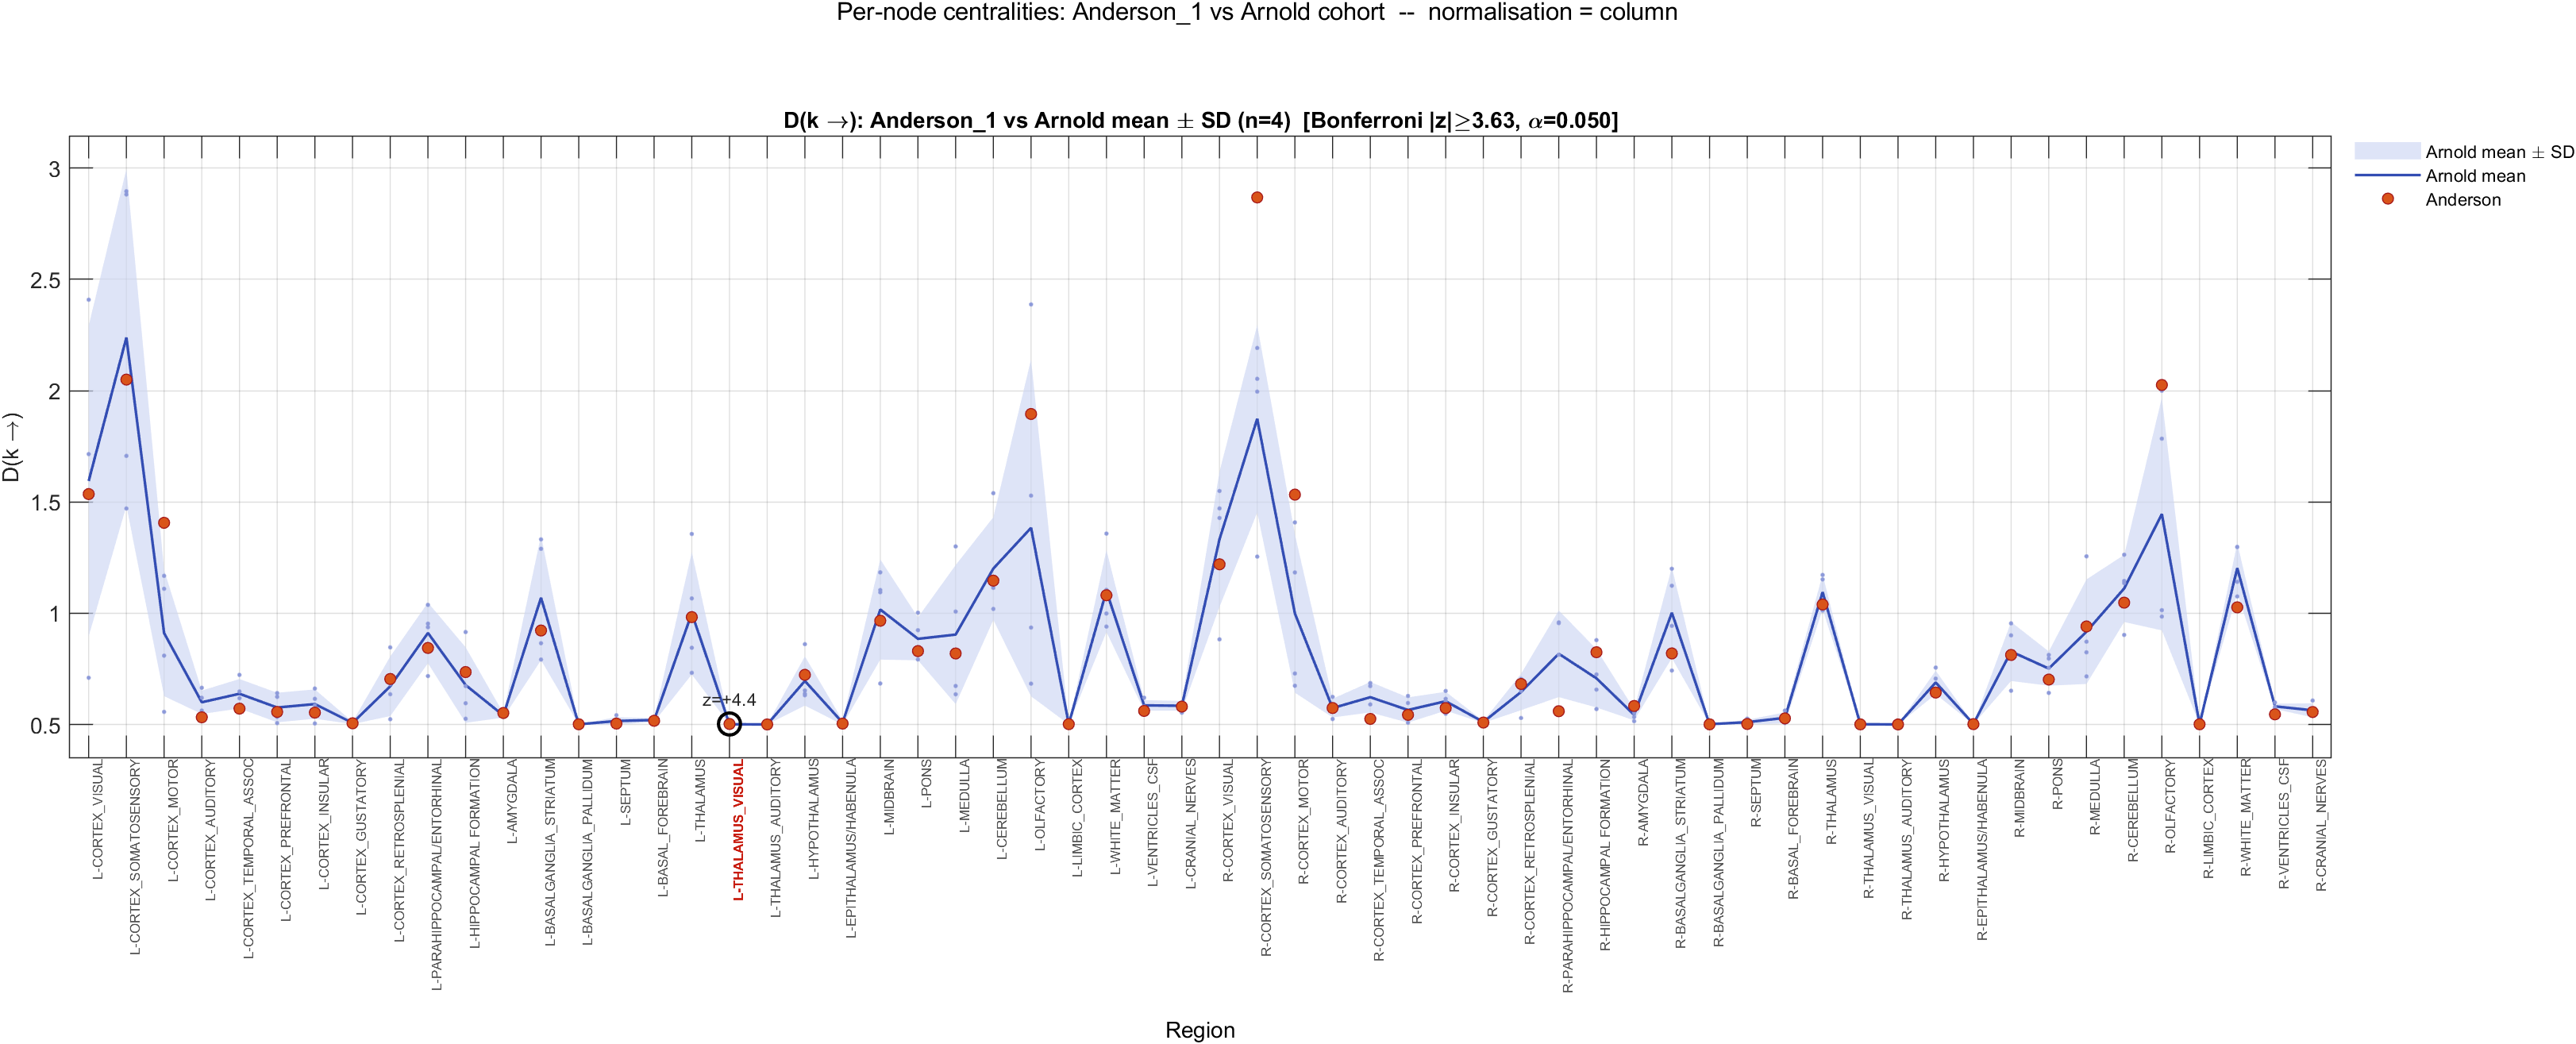
\includegraphics[width=\linewidth]{appendix/compare_anderson_vs_arnold_Anderson_1_column_D_k_to.png}
\caption{\textsc{Anderson\_1}, $\Dfrom$}
\end{subfigure}\hfill
\begin{subfigure}{0.32\textwidth}\centering
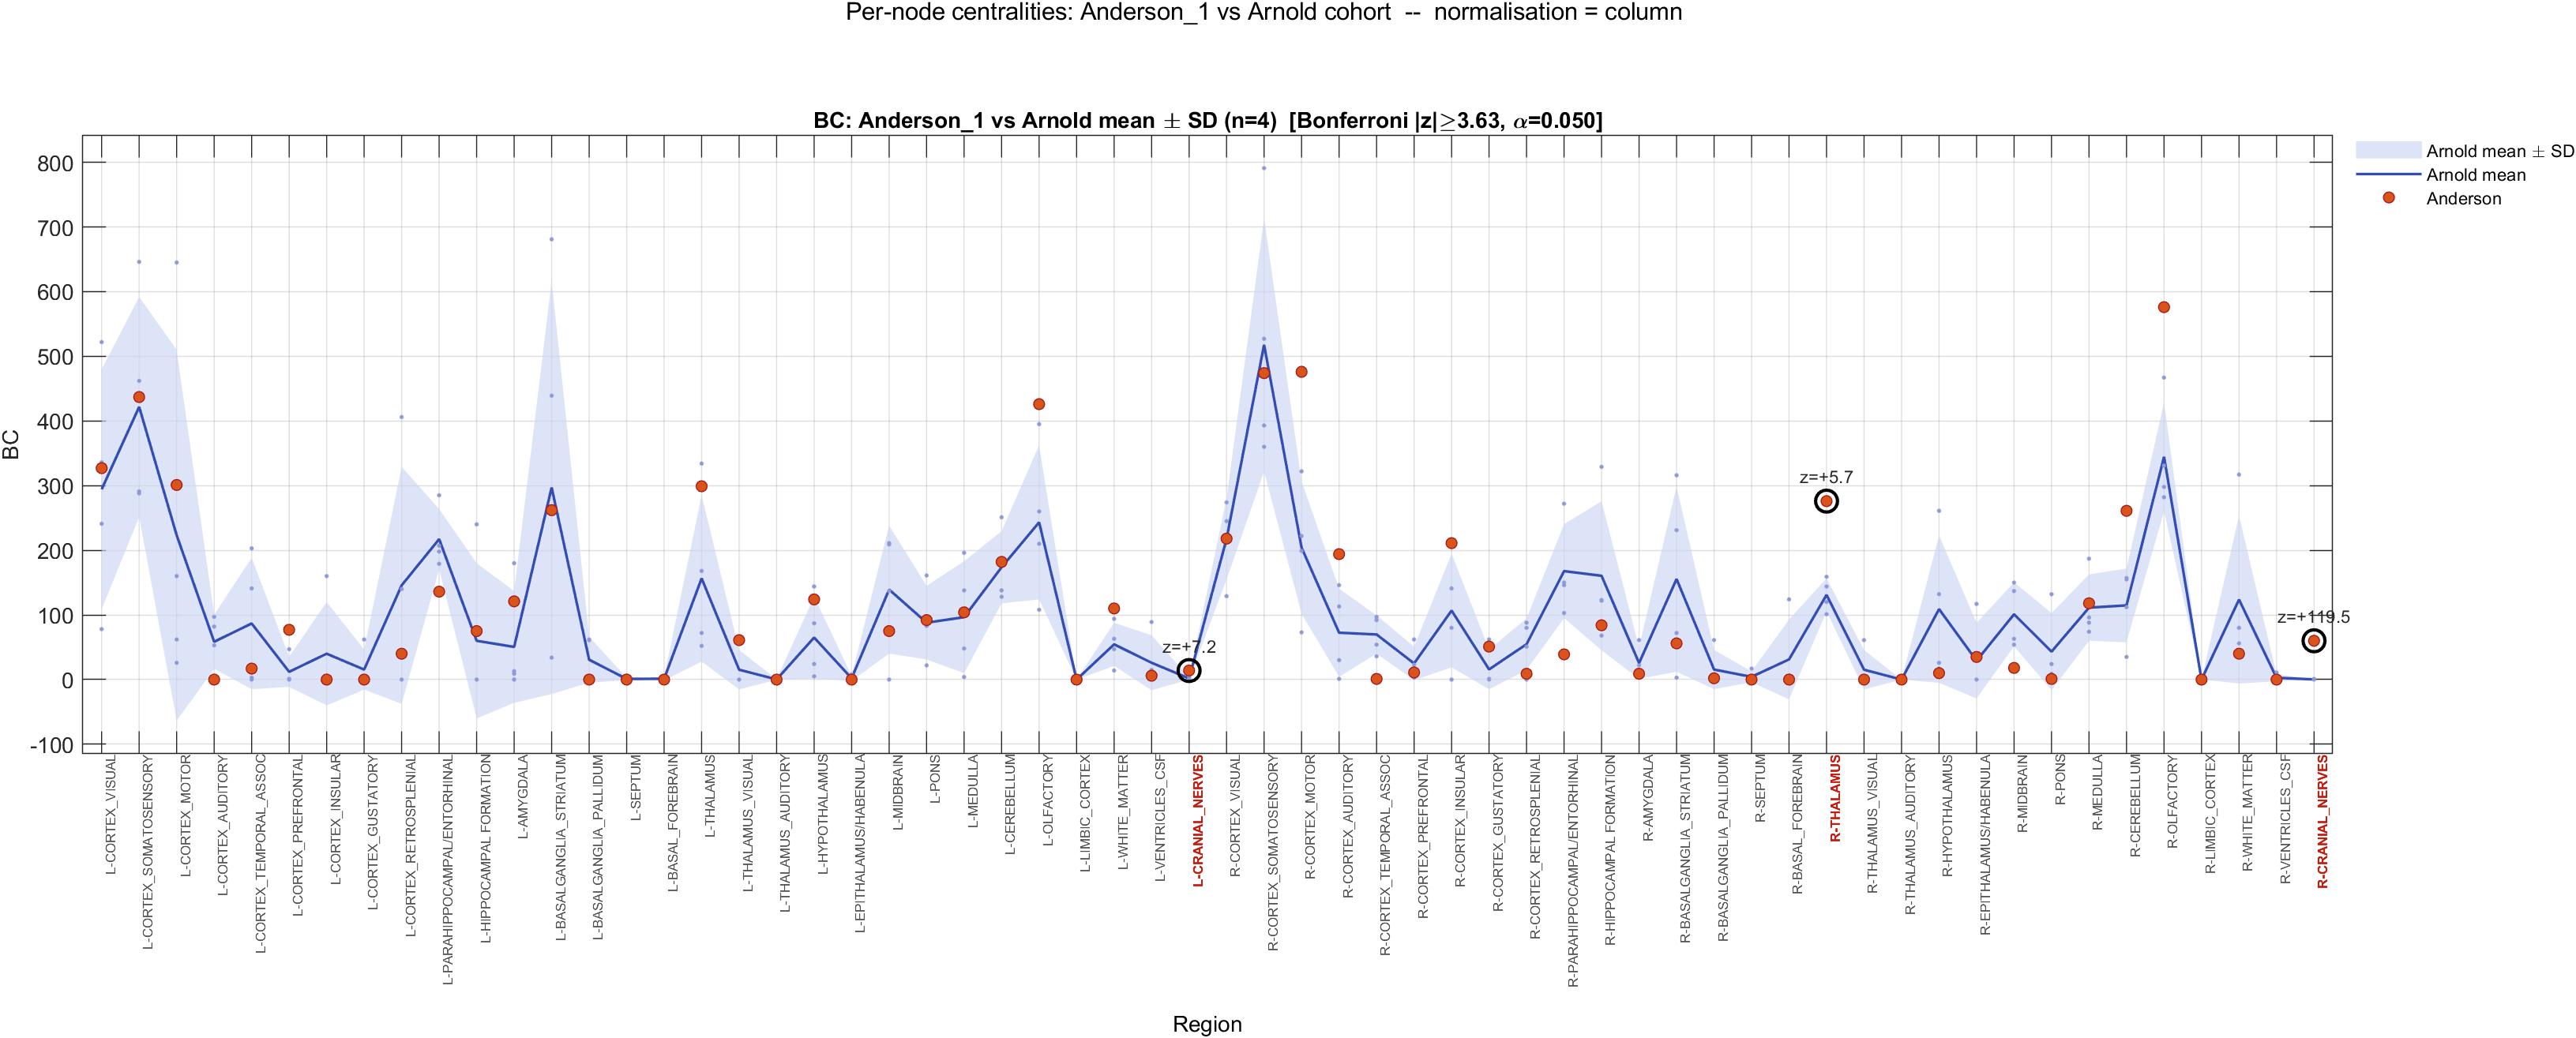
\includegraphics[width=\linewidth]{appendix/compare_anderson_vs_arnold_Anderson_1_column_BC.png}
\caption{\textsc{Anderson\_1}, BC}
\end{subfigure}\hfill
\begin{subfigure}{0.32\textwidth}\centering
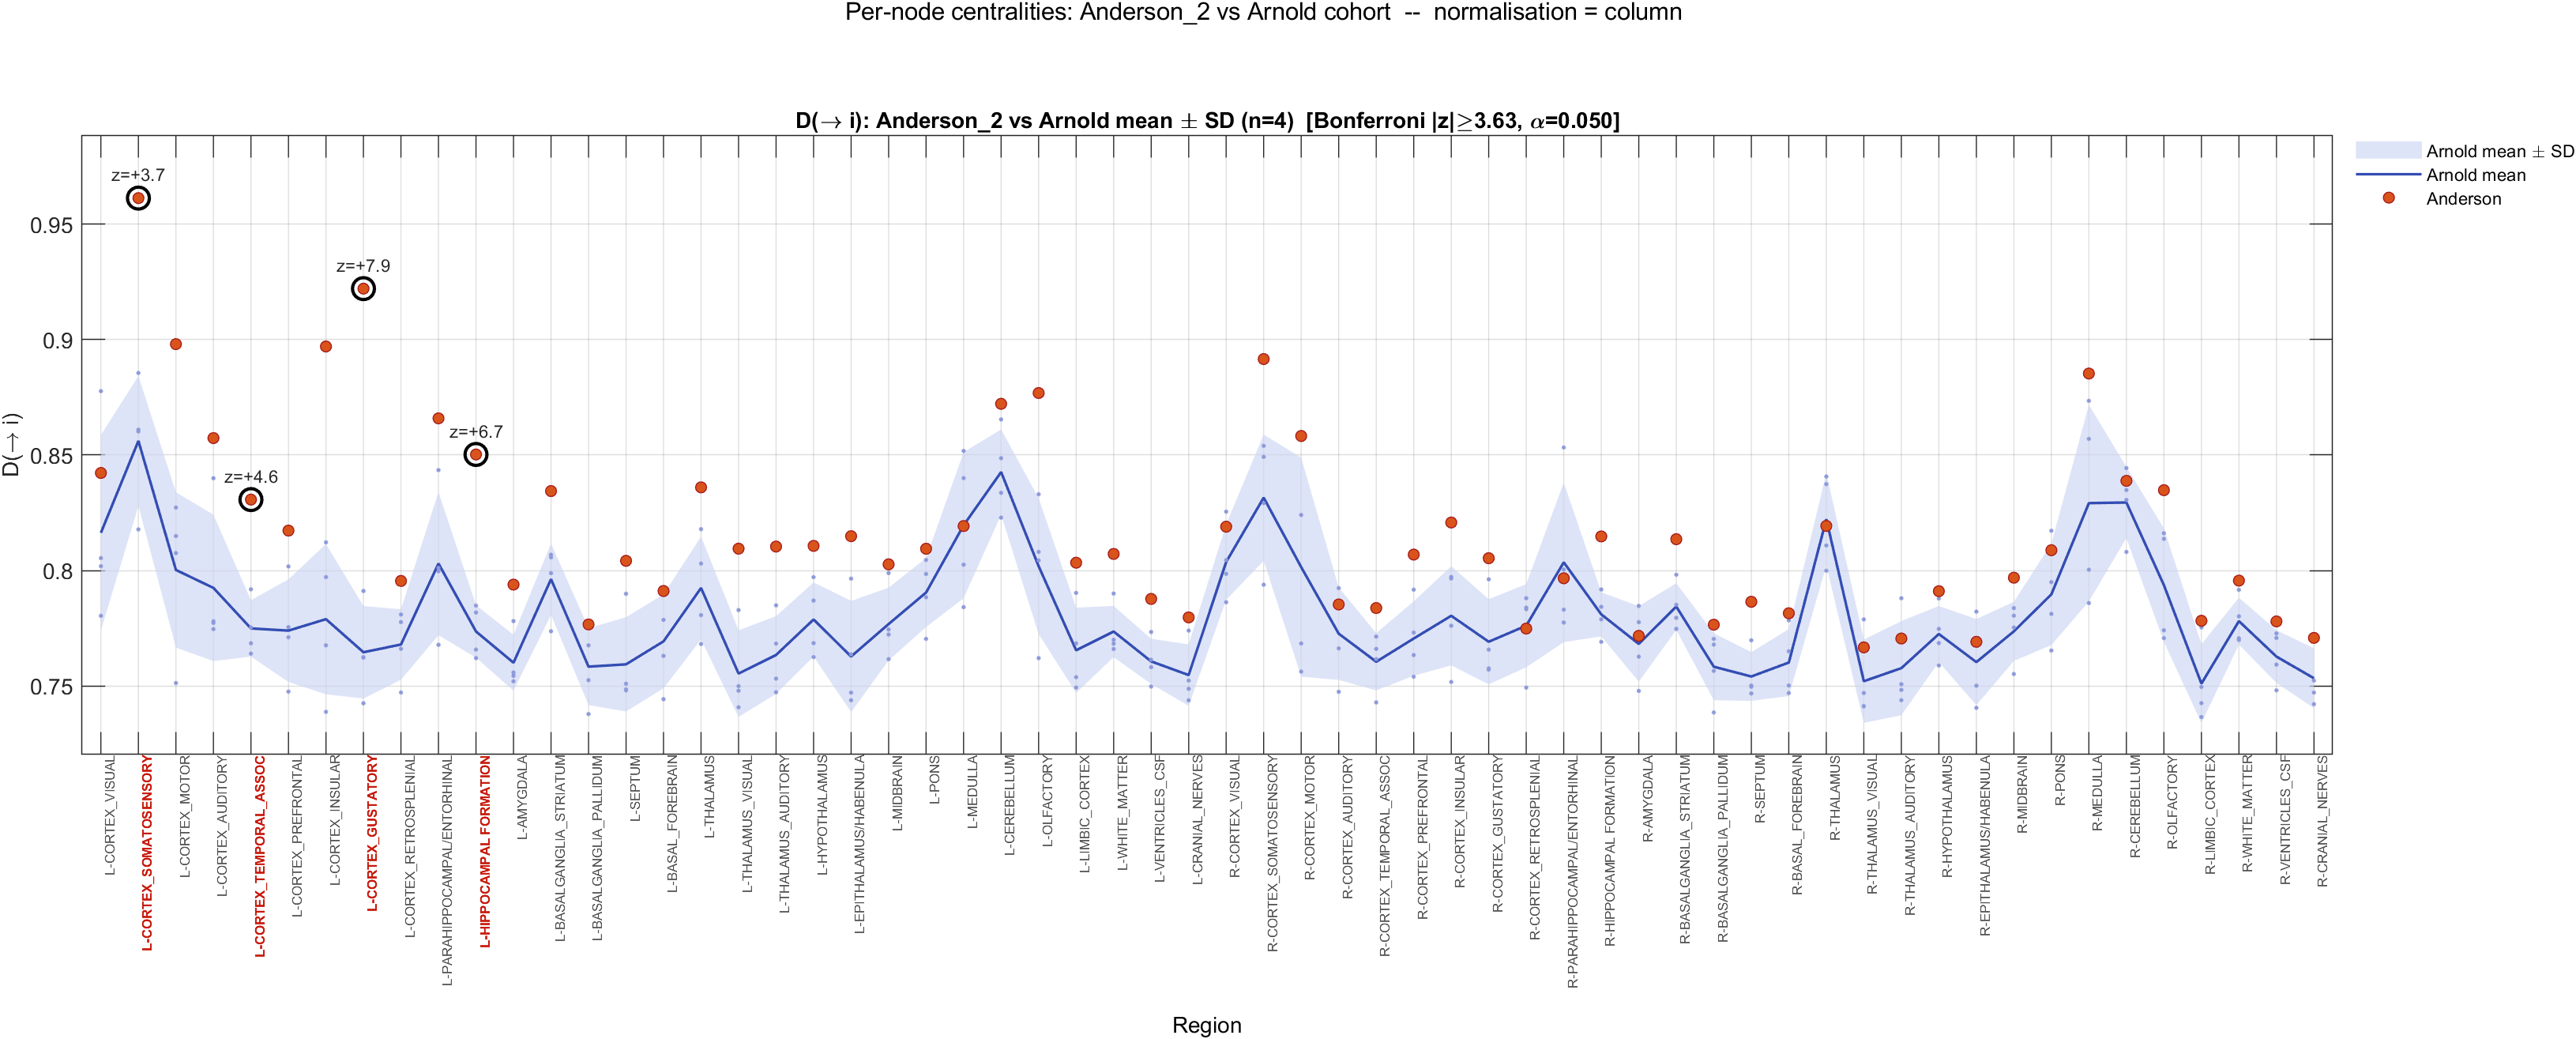
\includegraphics[width=\linewidth]{appendix/compare_anderson_vs_arnold_Anderson_2_column_D_to_i.png}
\caption{\textsc{Anderson\_2}, $\Dto$}
\end{subfigure}\hfill
\begin{subfigure}{0.32\textwidth}\centering
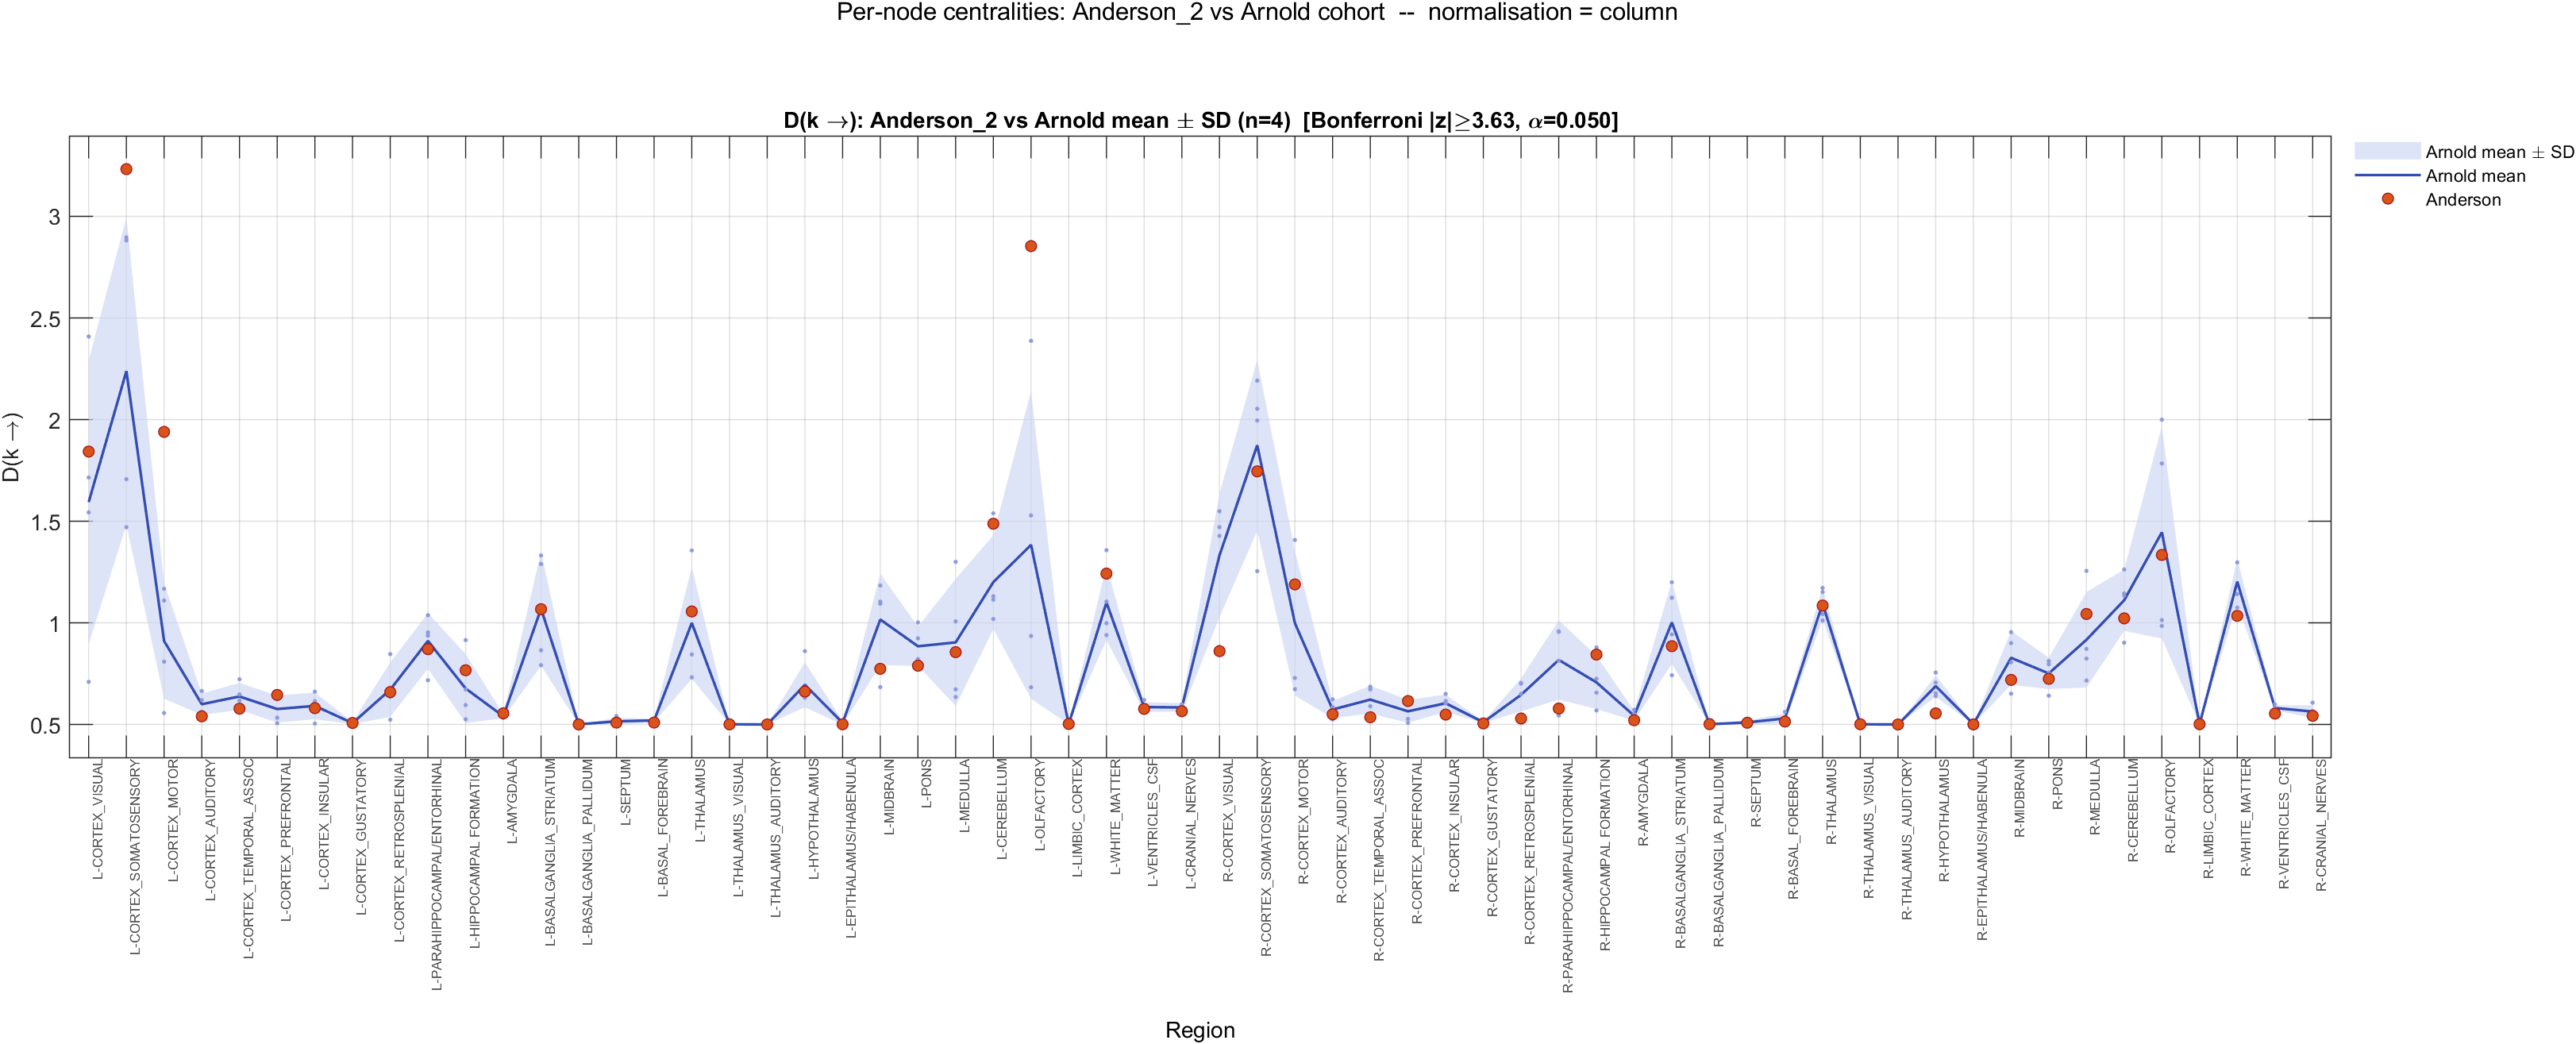
\includegraphics[width=\linewidth]{appendix/compare_anderson_vs_arnold_Anderson_2_column_D_k_to.png}
\caption{\textsc{Anderson\_2}, $\Dfrom$}
\end{subfigure}\hfill
\begin{subfigure}{0.32\textwidth}\centering
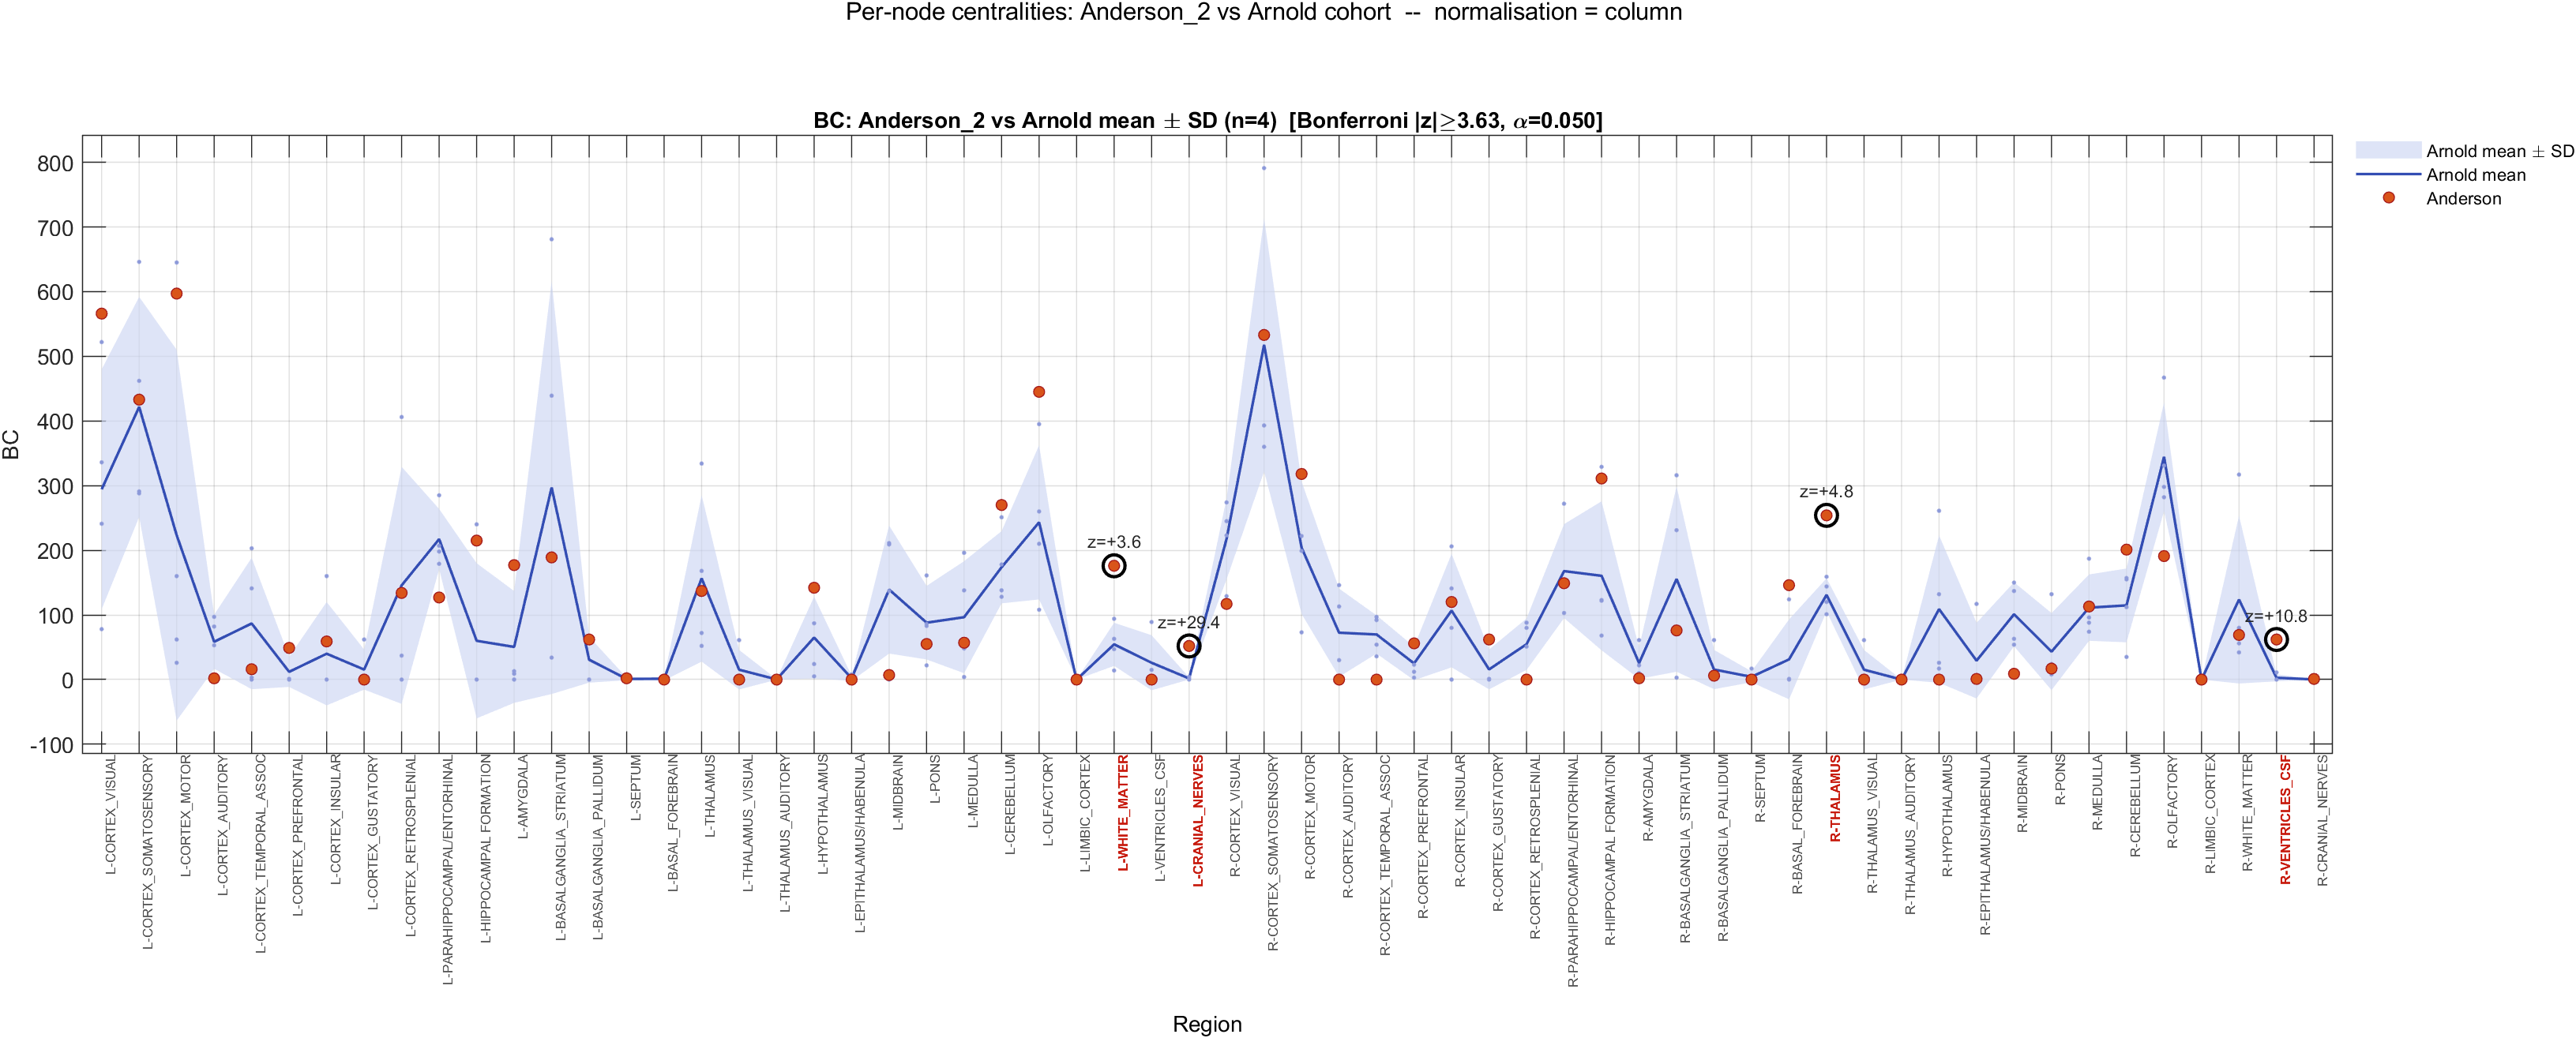
\includegraphics[width=\linewidth]{appendix/compare_anderson_vs_arnold_Anderson_2_column_BC.png}
\caption{\textsc{Anderson\_2}, BC}
\end{subfigure}\hfill
\caption{Each case mouse against the four-control band, \texttt{column} scheme: susceptibility $\Dto$, influence $\Dfrom$, and betweenness BC.}
\end{figure}

\begin{figure}[H]\centering
\begin{subfigure}{0.32\textwidth}\centering
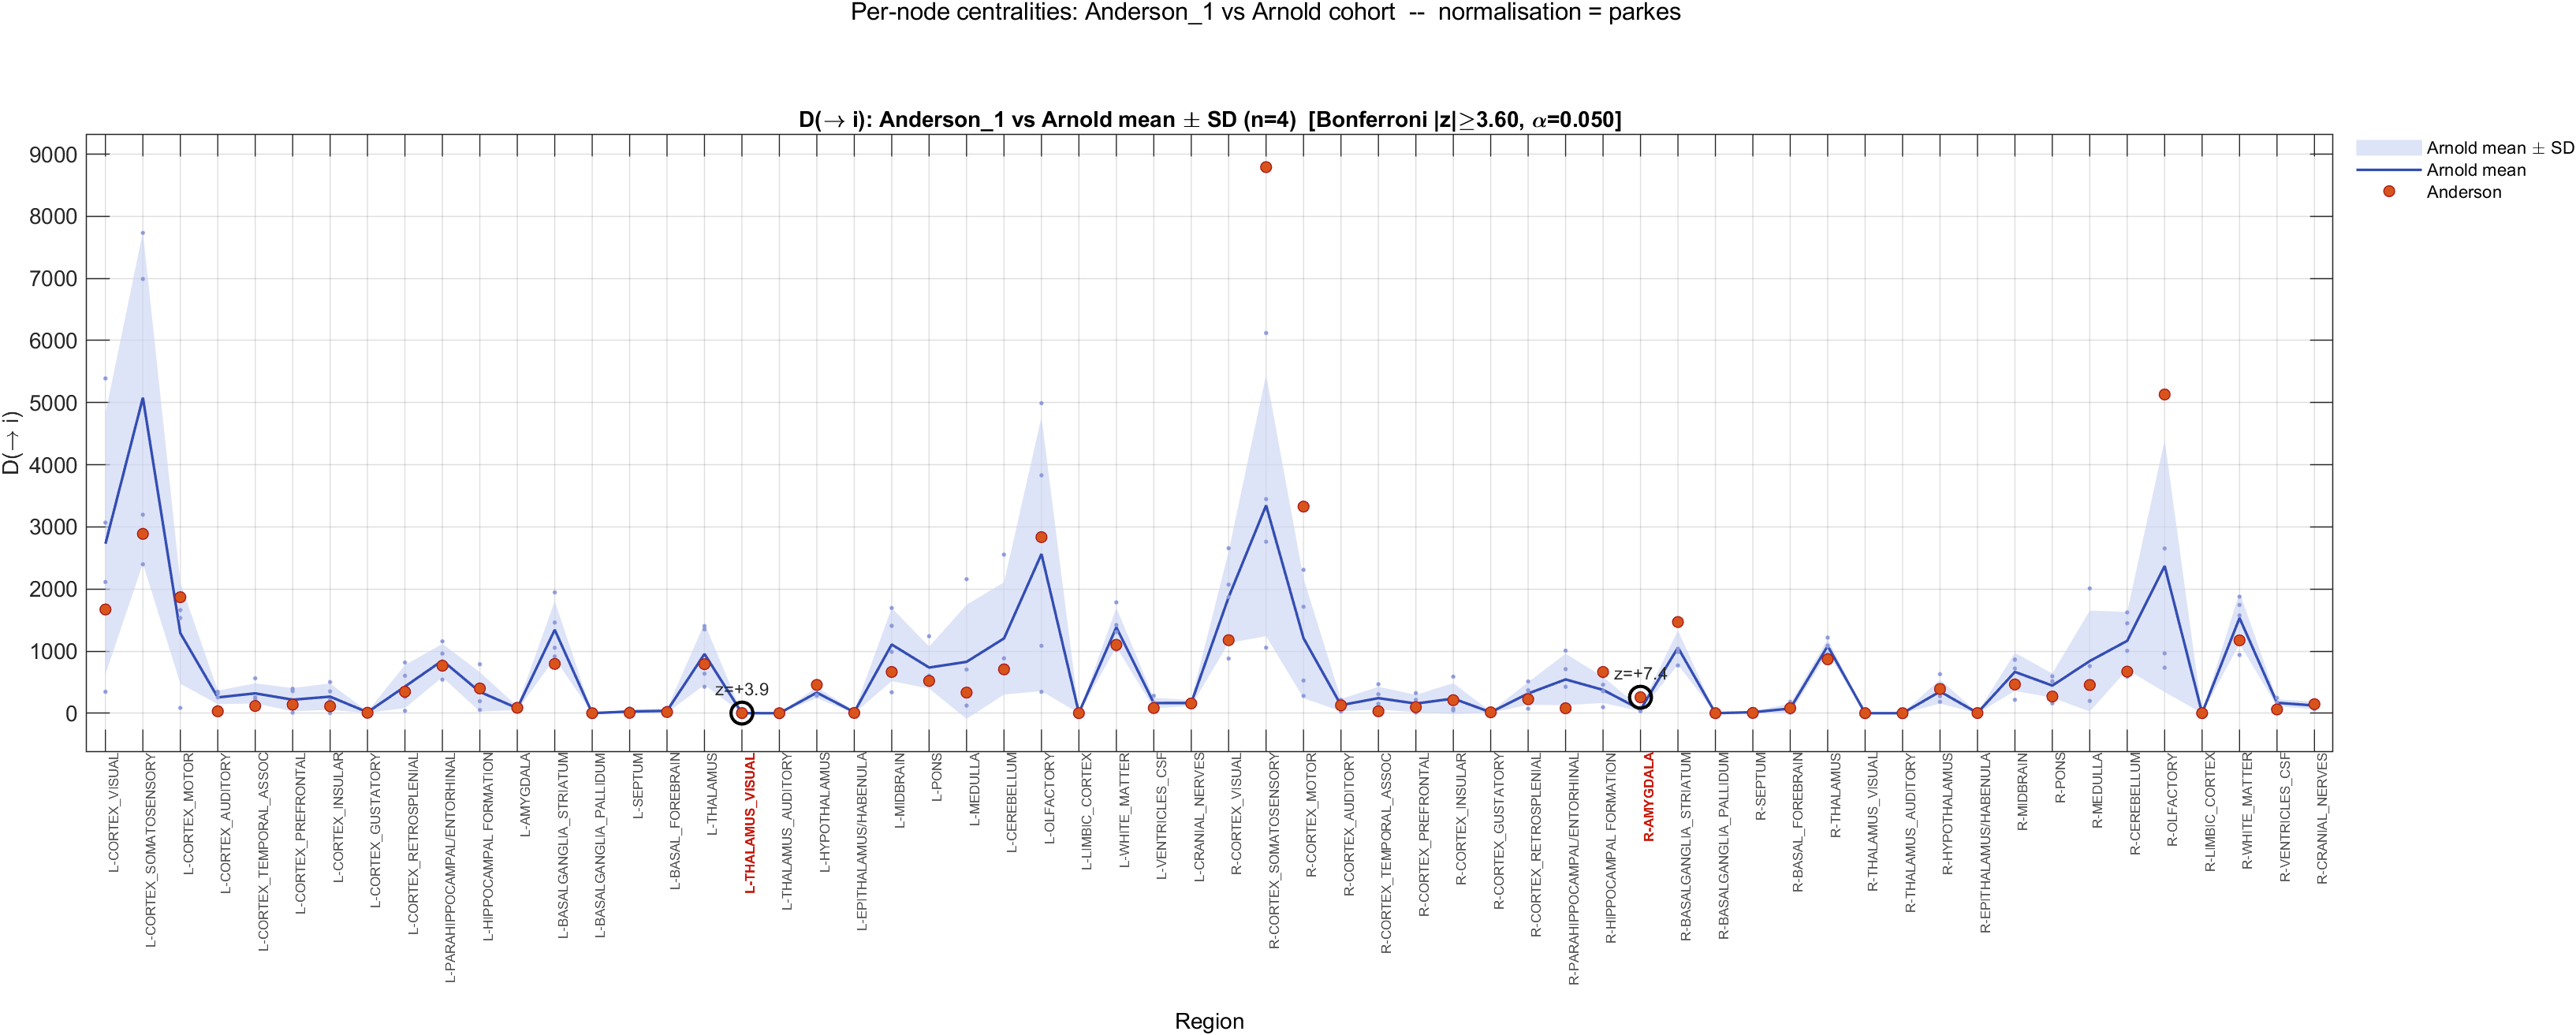
\includegraphics[width=\linewidth]{appendix/compare_anderson_vs_arnold_Anderson_1_parkes_D_to_i.png}
\caption{\textsc{Anderson\_1}, $\Dto$}
\end{subfigure}\hfill
\begin{subfigure}{0.32\textwidth}\centering
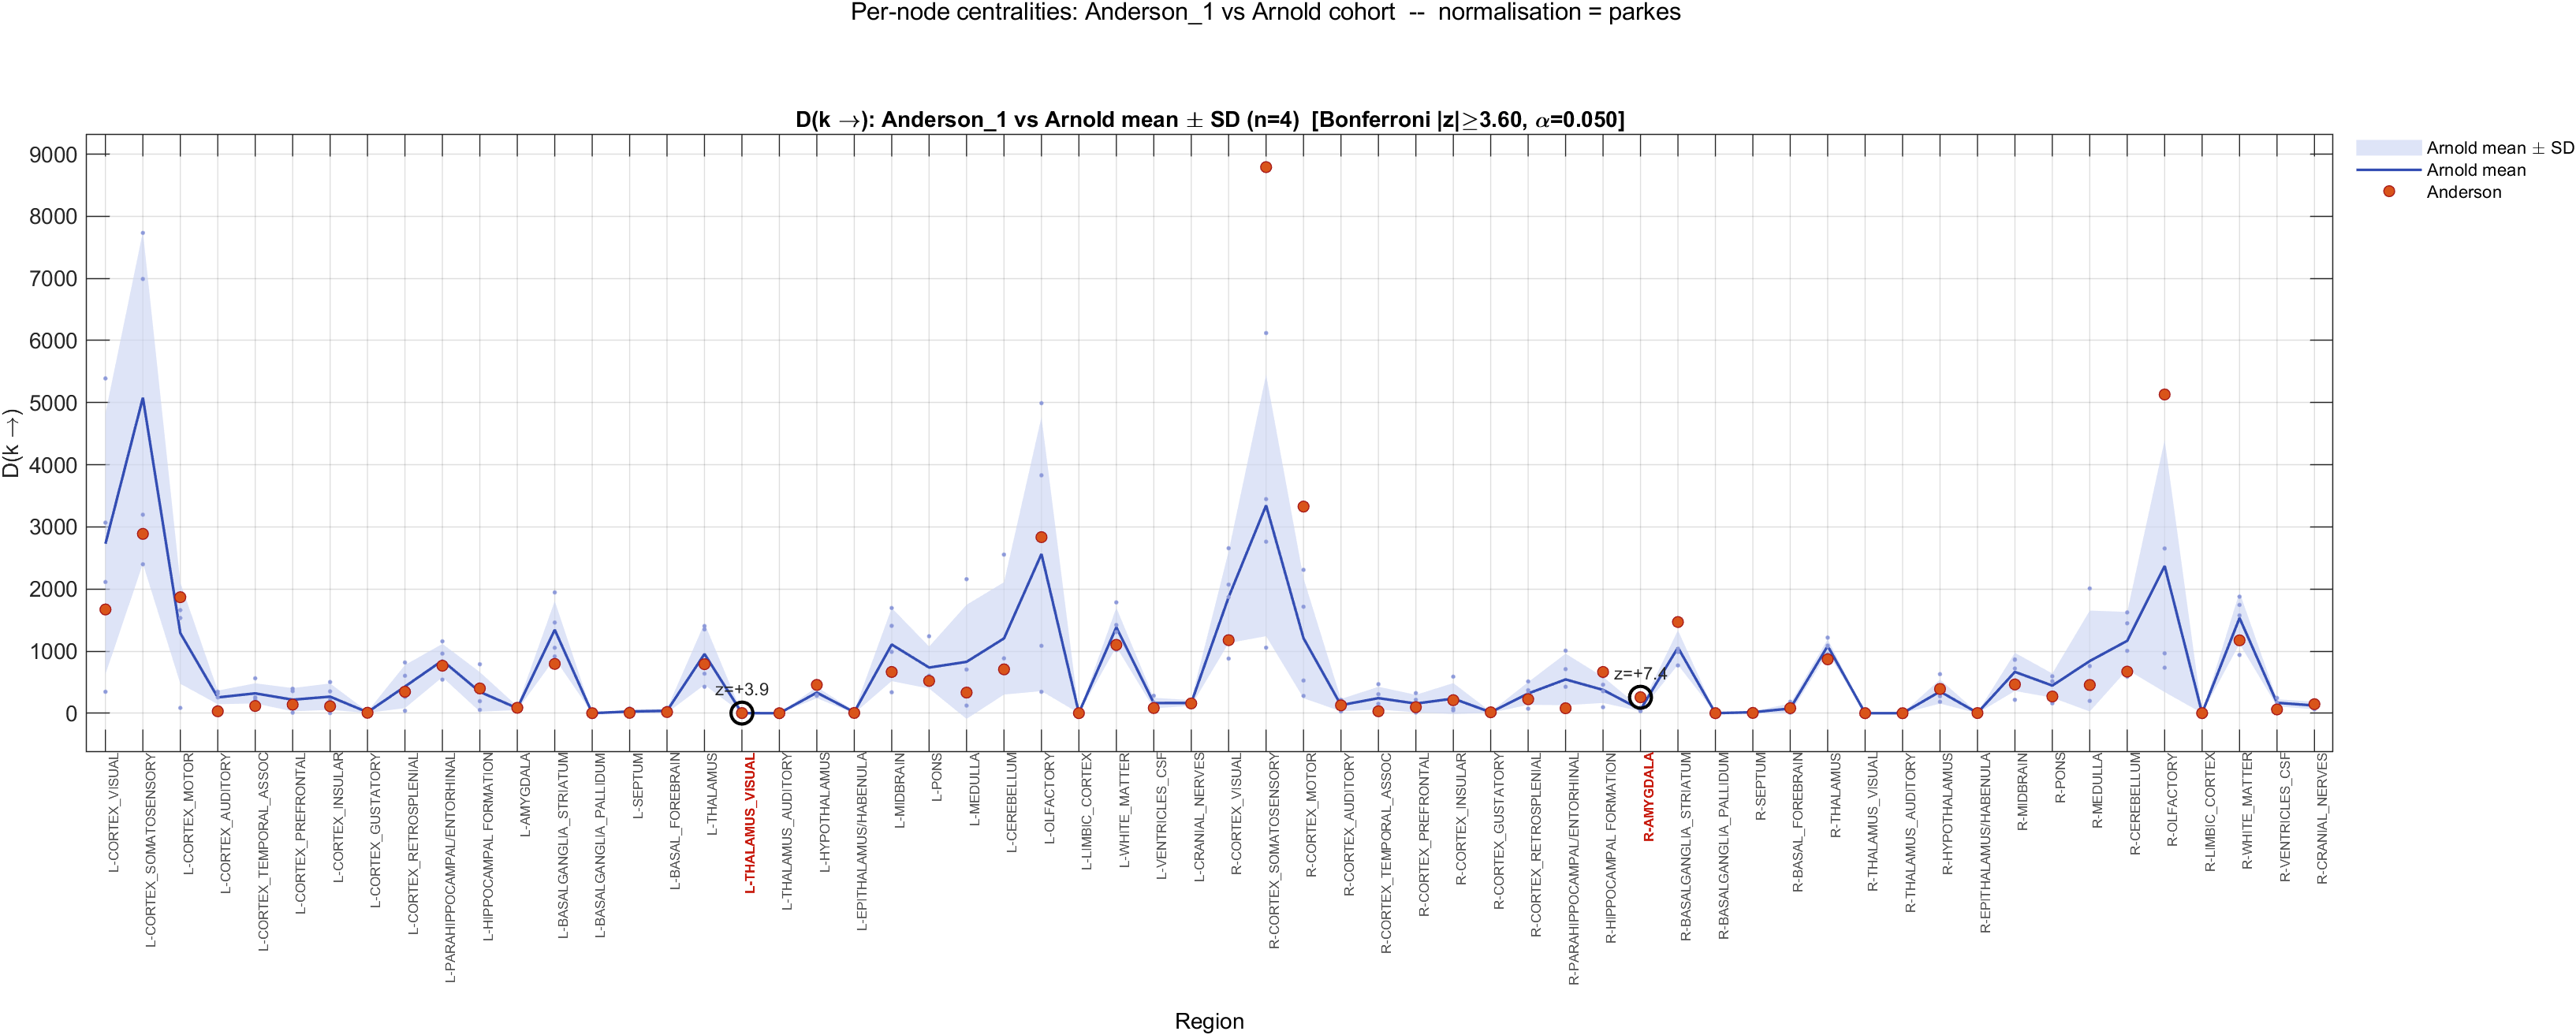
\includegraphics[width=\linewidth]{appendix/compare_anderson_vs_arnold_Anderson_1_parkes_D_k_to.png}
\caption{\textsc{Anderson\_1}, $\Dfrom$}
\end{subfigure}\hfill
\begin{subfigure}{0.32\textwidth}\centering
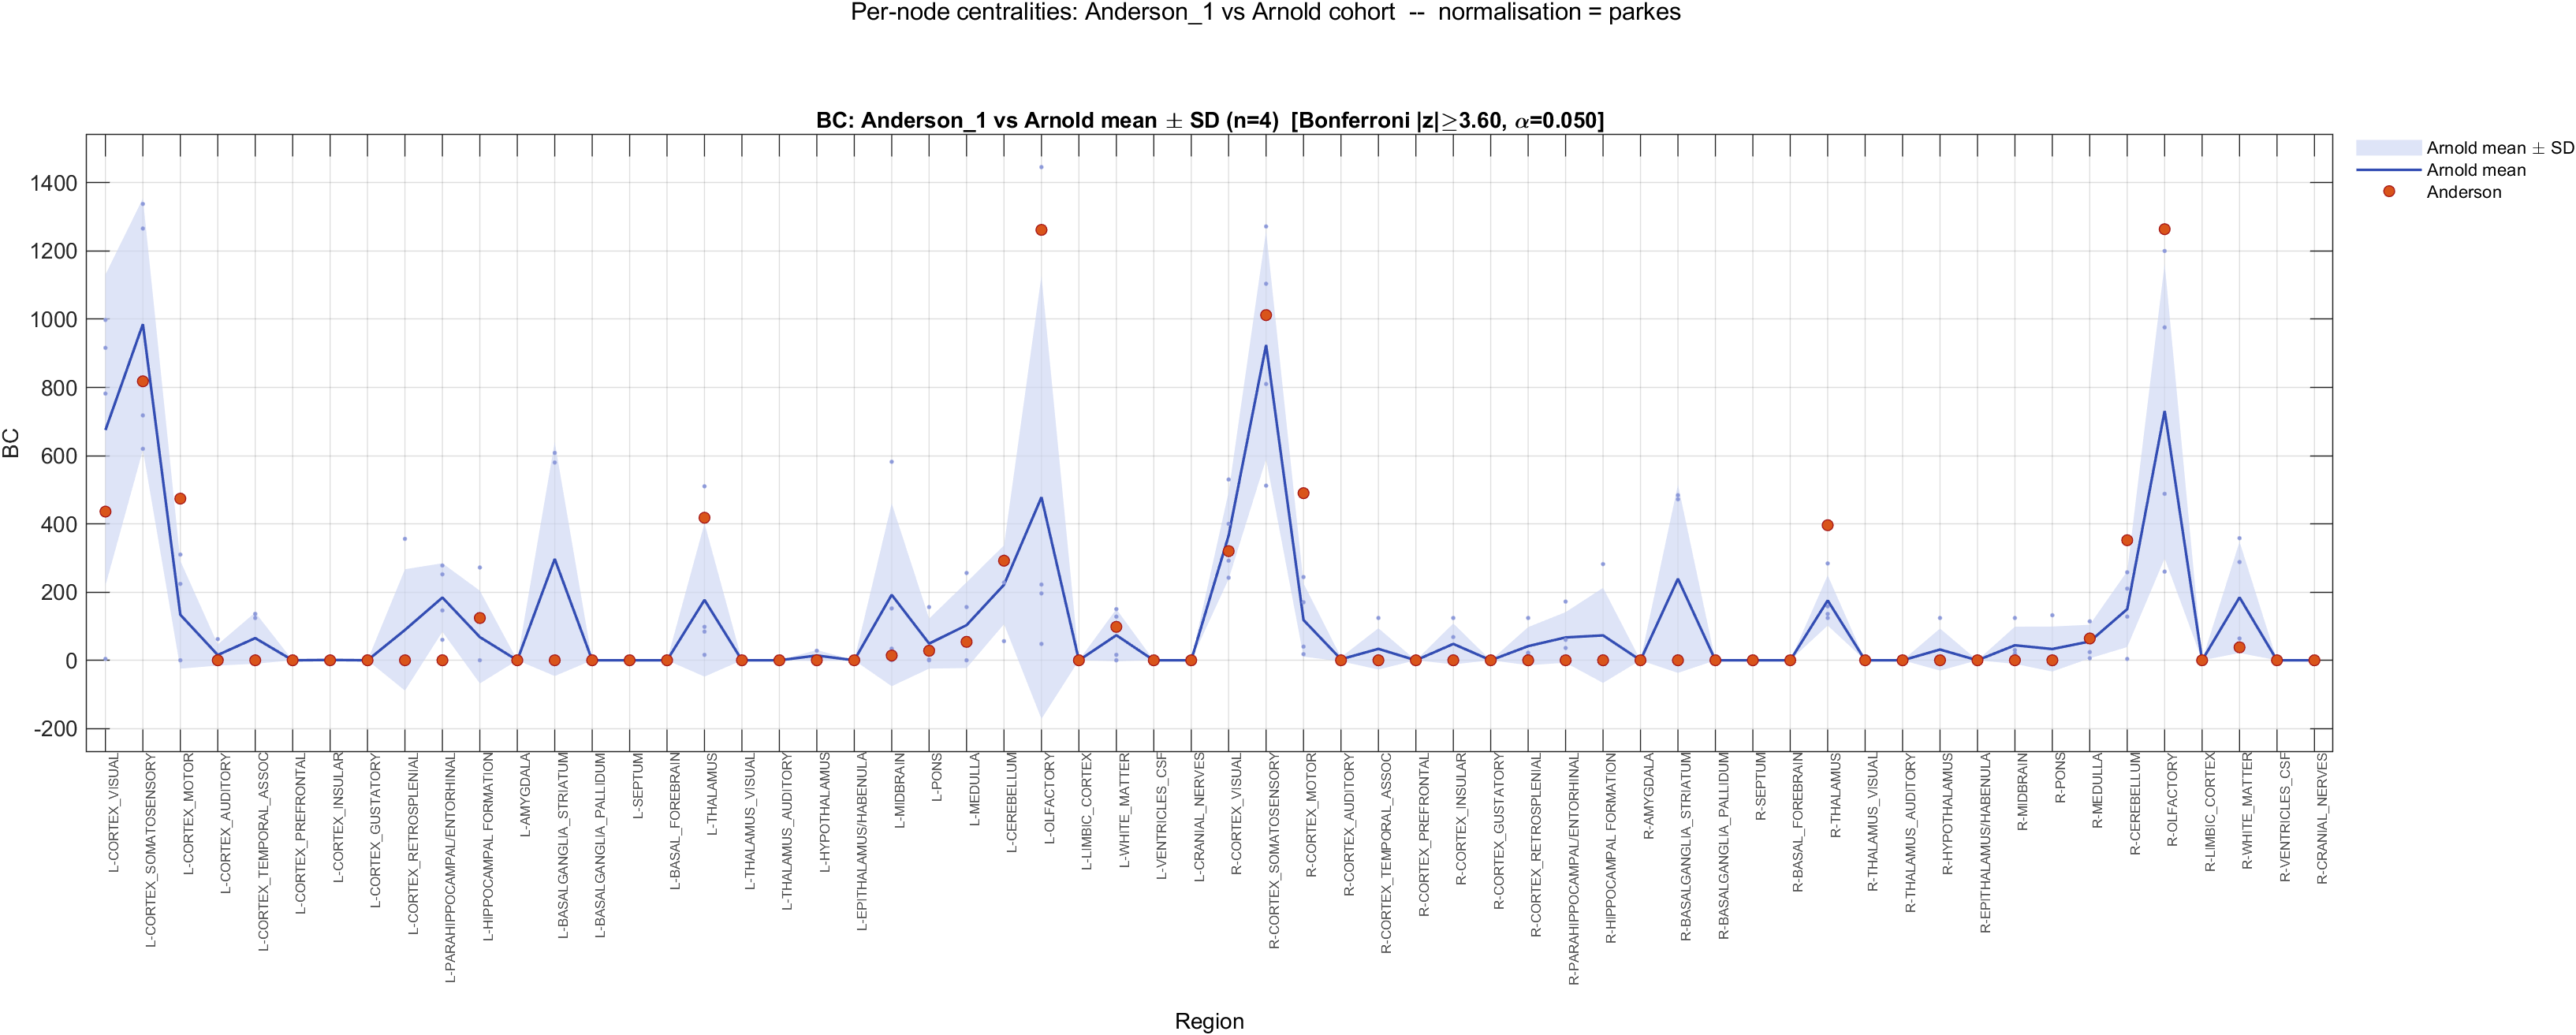
\includegraphics[width=\linewidth]{appendix/compare_anderson_vs_arnold_Anderson_1_parkes_BC.png}
\caption{\textsc{Anderson\_1}, BC}
\end{subfigure}\hfill
\begin{subfigure}{0.32\textwidth}\centering
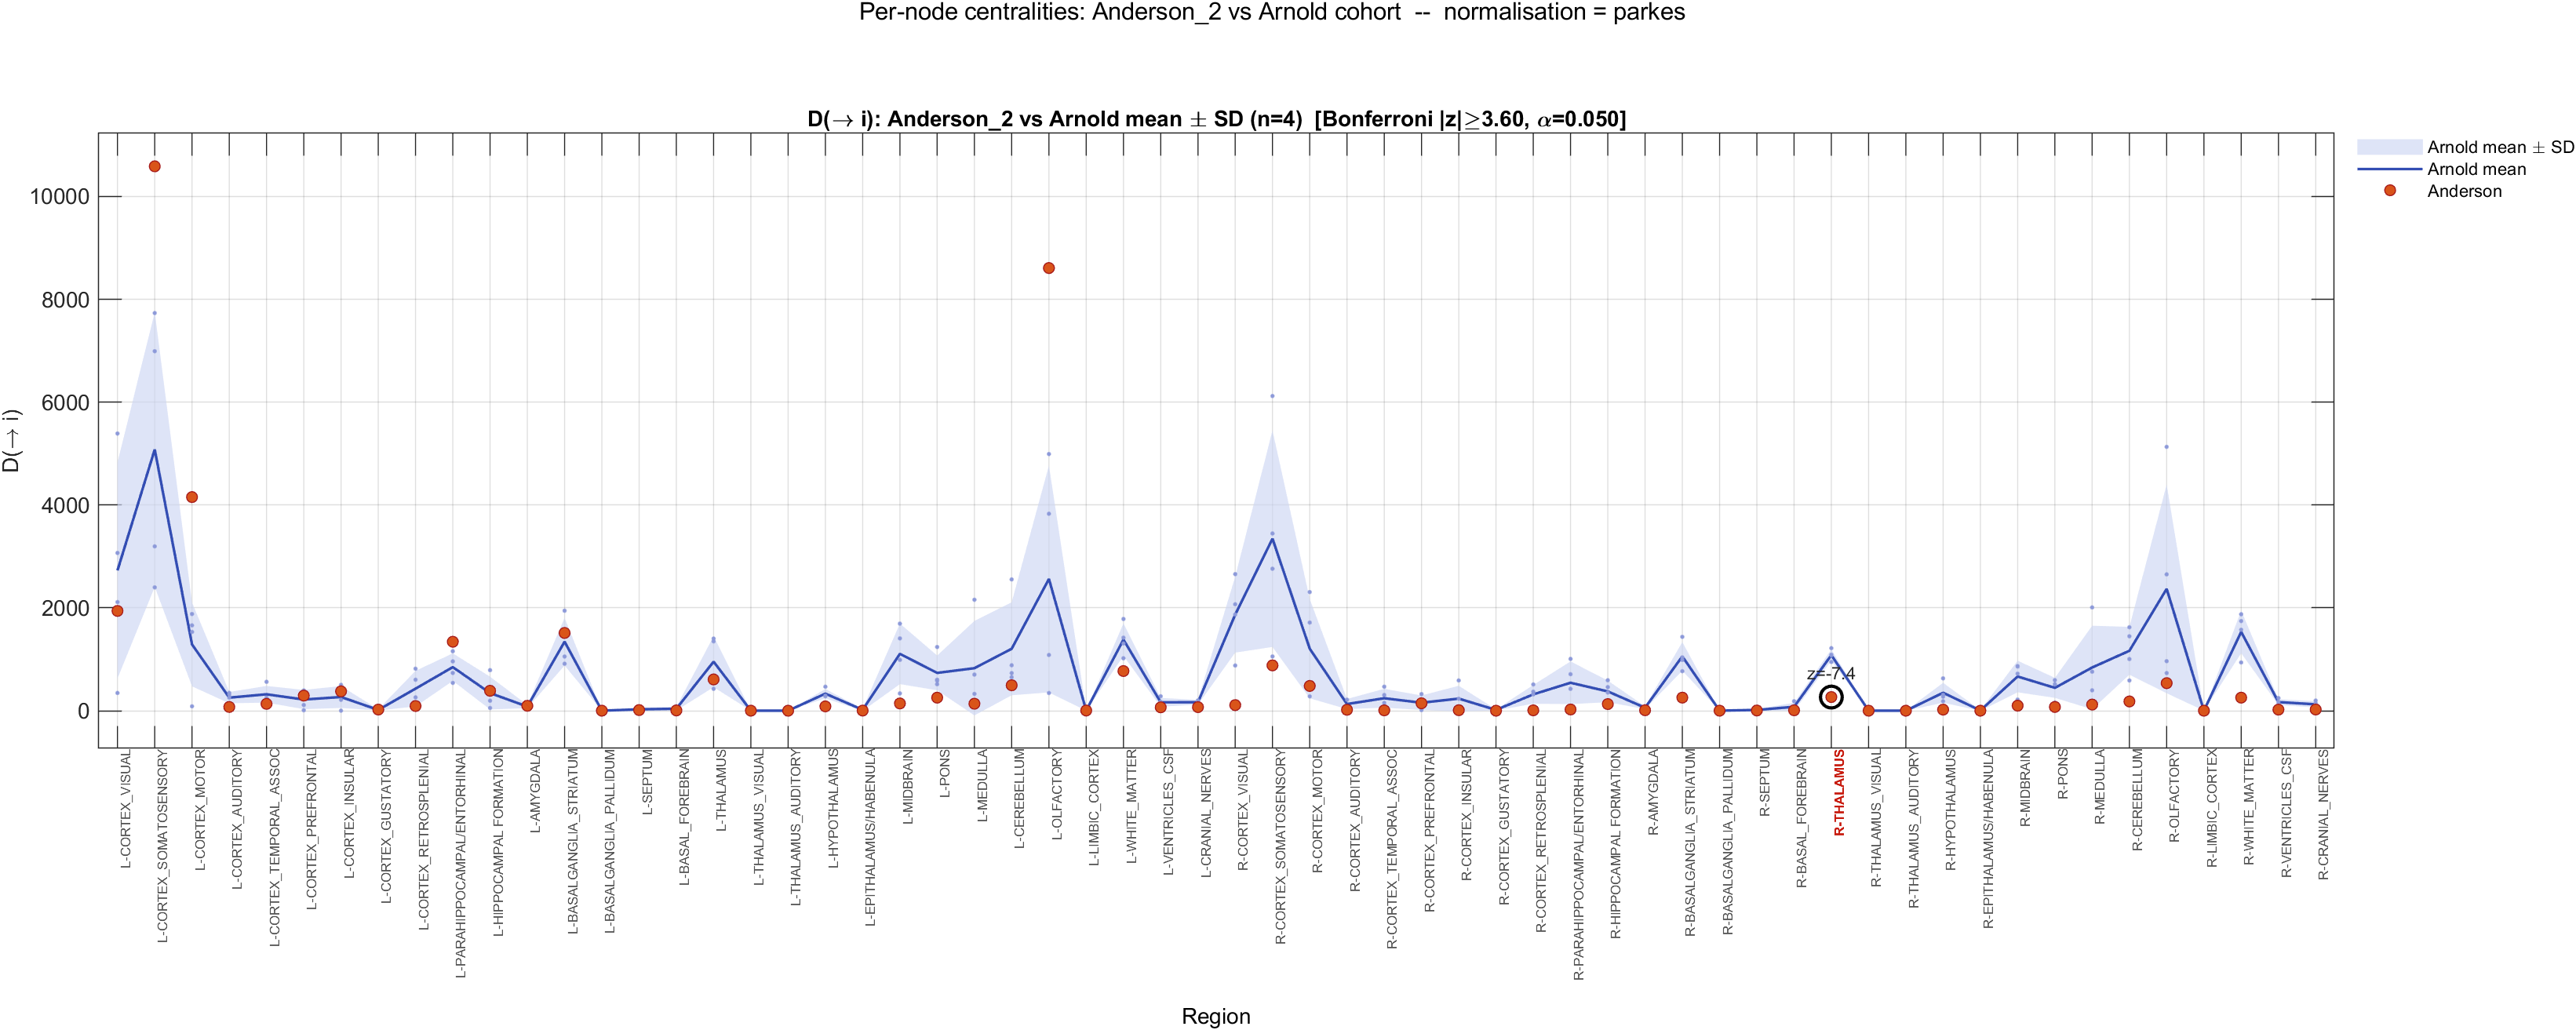
\includegraphics[width=\linewidth]{appendix/compare_anderson_vs_arnold_Anderson_2_parkes_D_to_i.png}
\caption{\textsc{Anderson\_2}, $\Dto$}
\end{subfigure}\hfill
\begin{subfigure}{0.32\textwidth}\centering
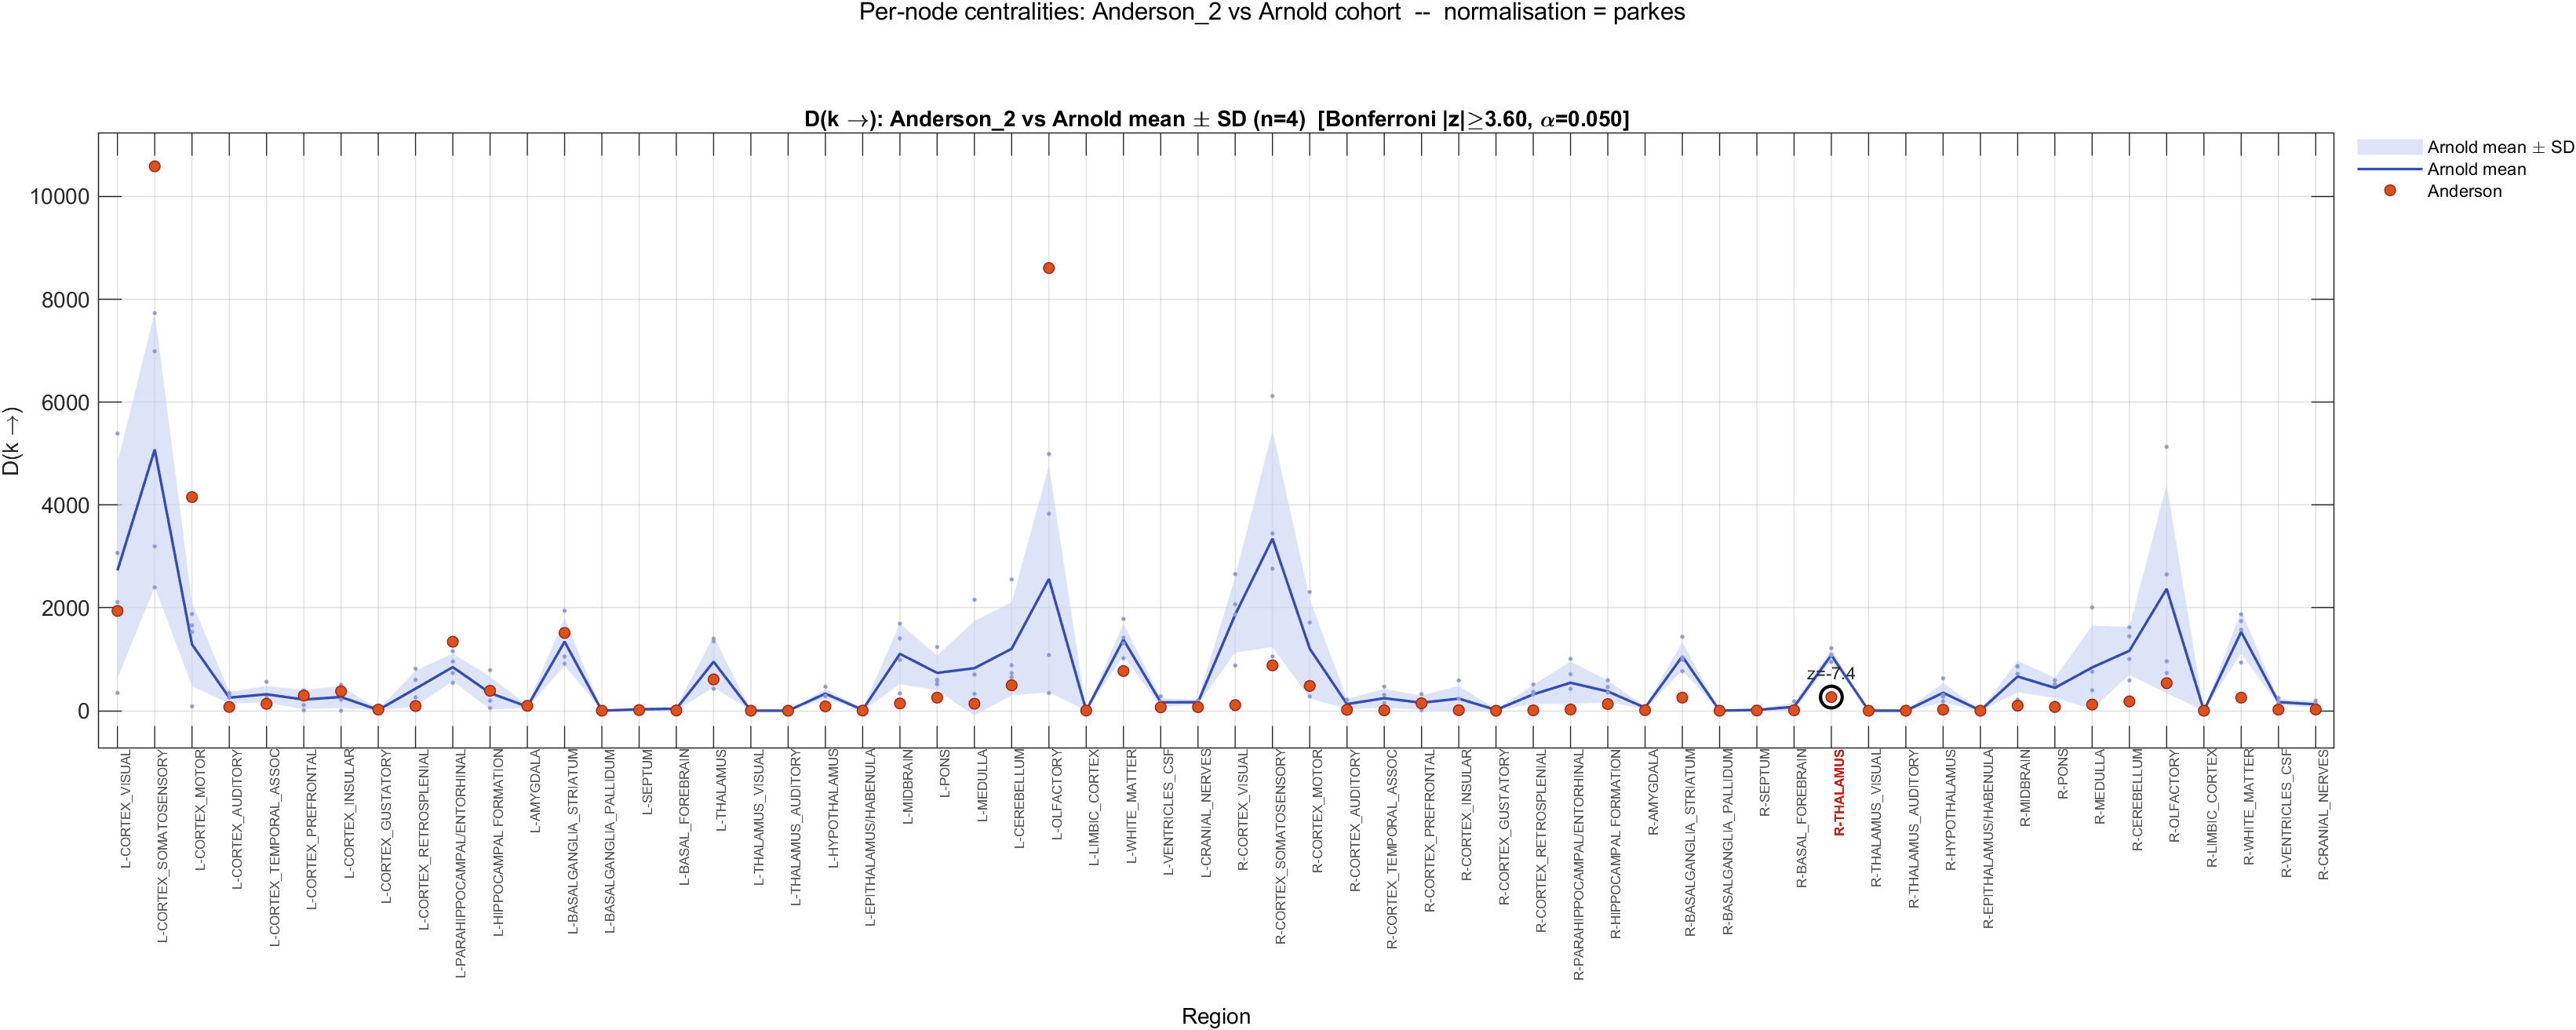
\includegraphics[width=\linewidth]{appendix/compare_anderson_vs_arnold_Anderson_2_parkes_D_k_to.png}
\caption{\textsc{Anderson\_2}, $\Dfrom$}
\end{subfigure}\hfill
\begin{subfigure}{0.32\textwidth}\centering
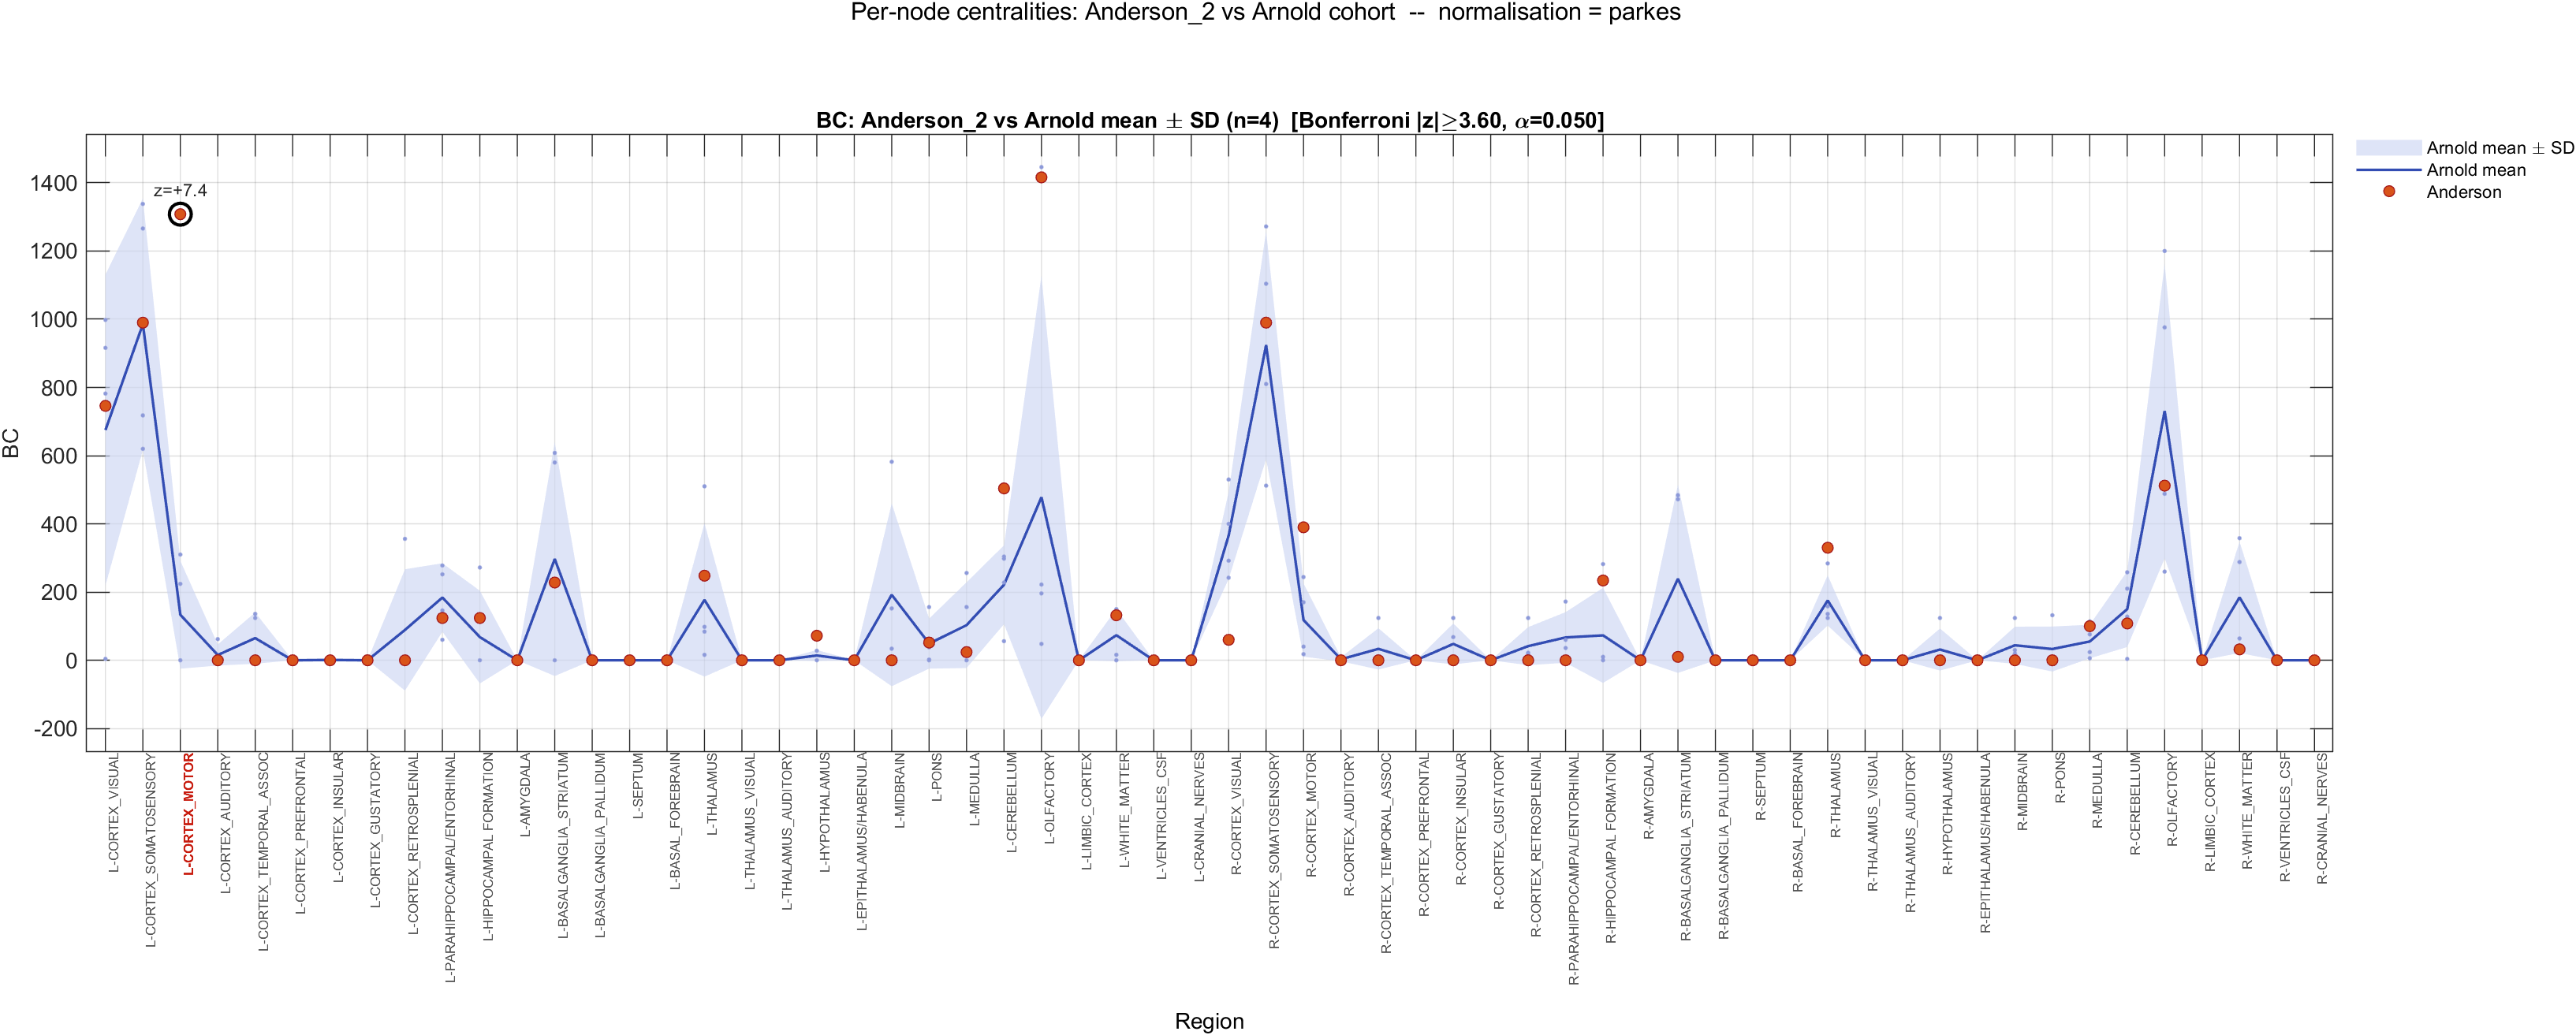
\includegraphics[width=\linewidth]{appendix/compare_anderson_vs_arnold_Anderson_2_parkes_BC.png}
\caption{\textsc{Anderson\_2}, BC}
\end{subfigure}\hfill
\caption{Each case mouse against the four-control band, \texttt{parkes} scheme: susceptibility $\Dto$, influence $\Dfrom$, and betweenness BC.}
\end{figure}

\begin{figure}[H]\centering
\begin{subfigure}{0.32\textwidth}\centering
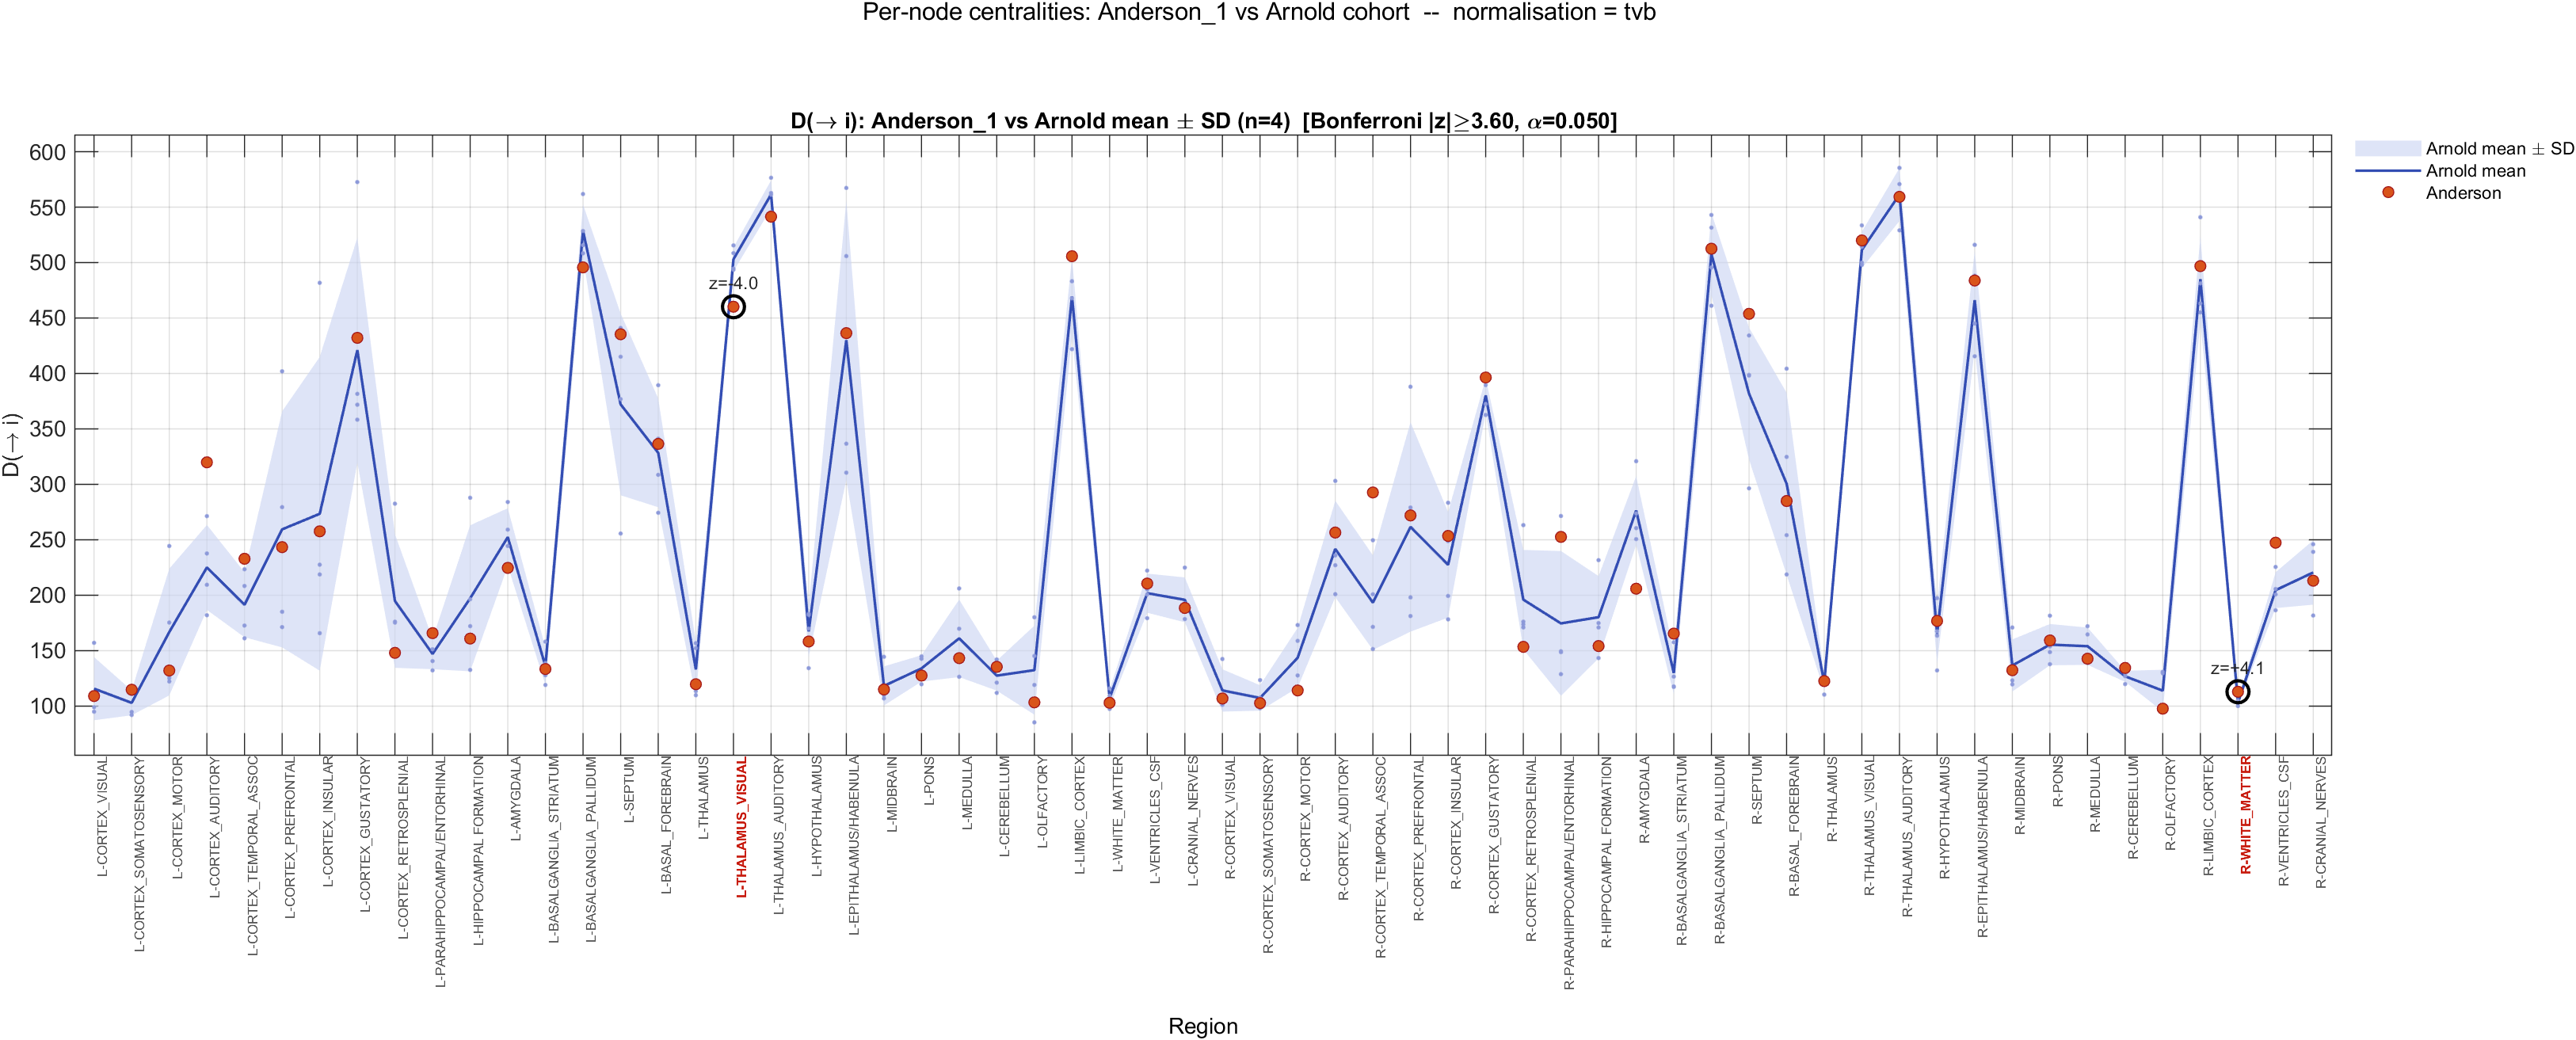
\includegraphics[width=\linewidth]{appendix/compare_anderson_vs_arnold_Anderson_1_tvb_D_to_i.png}
\caption{\textsc{Anderson\_1}, $\Dto$}
\end{subfigure}\hfill
\begin{subfigure}{0.32\textwidth}\centering
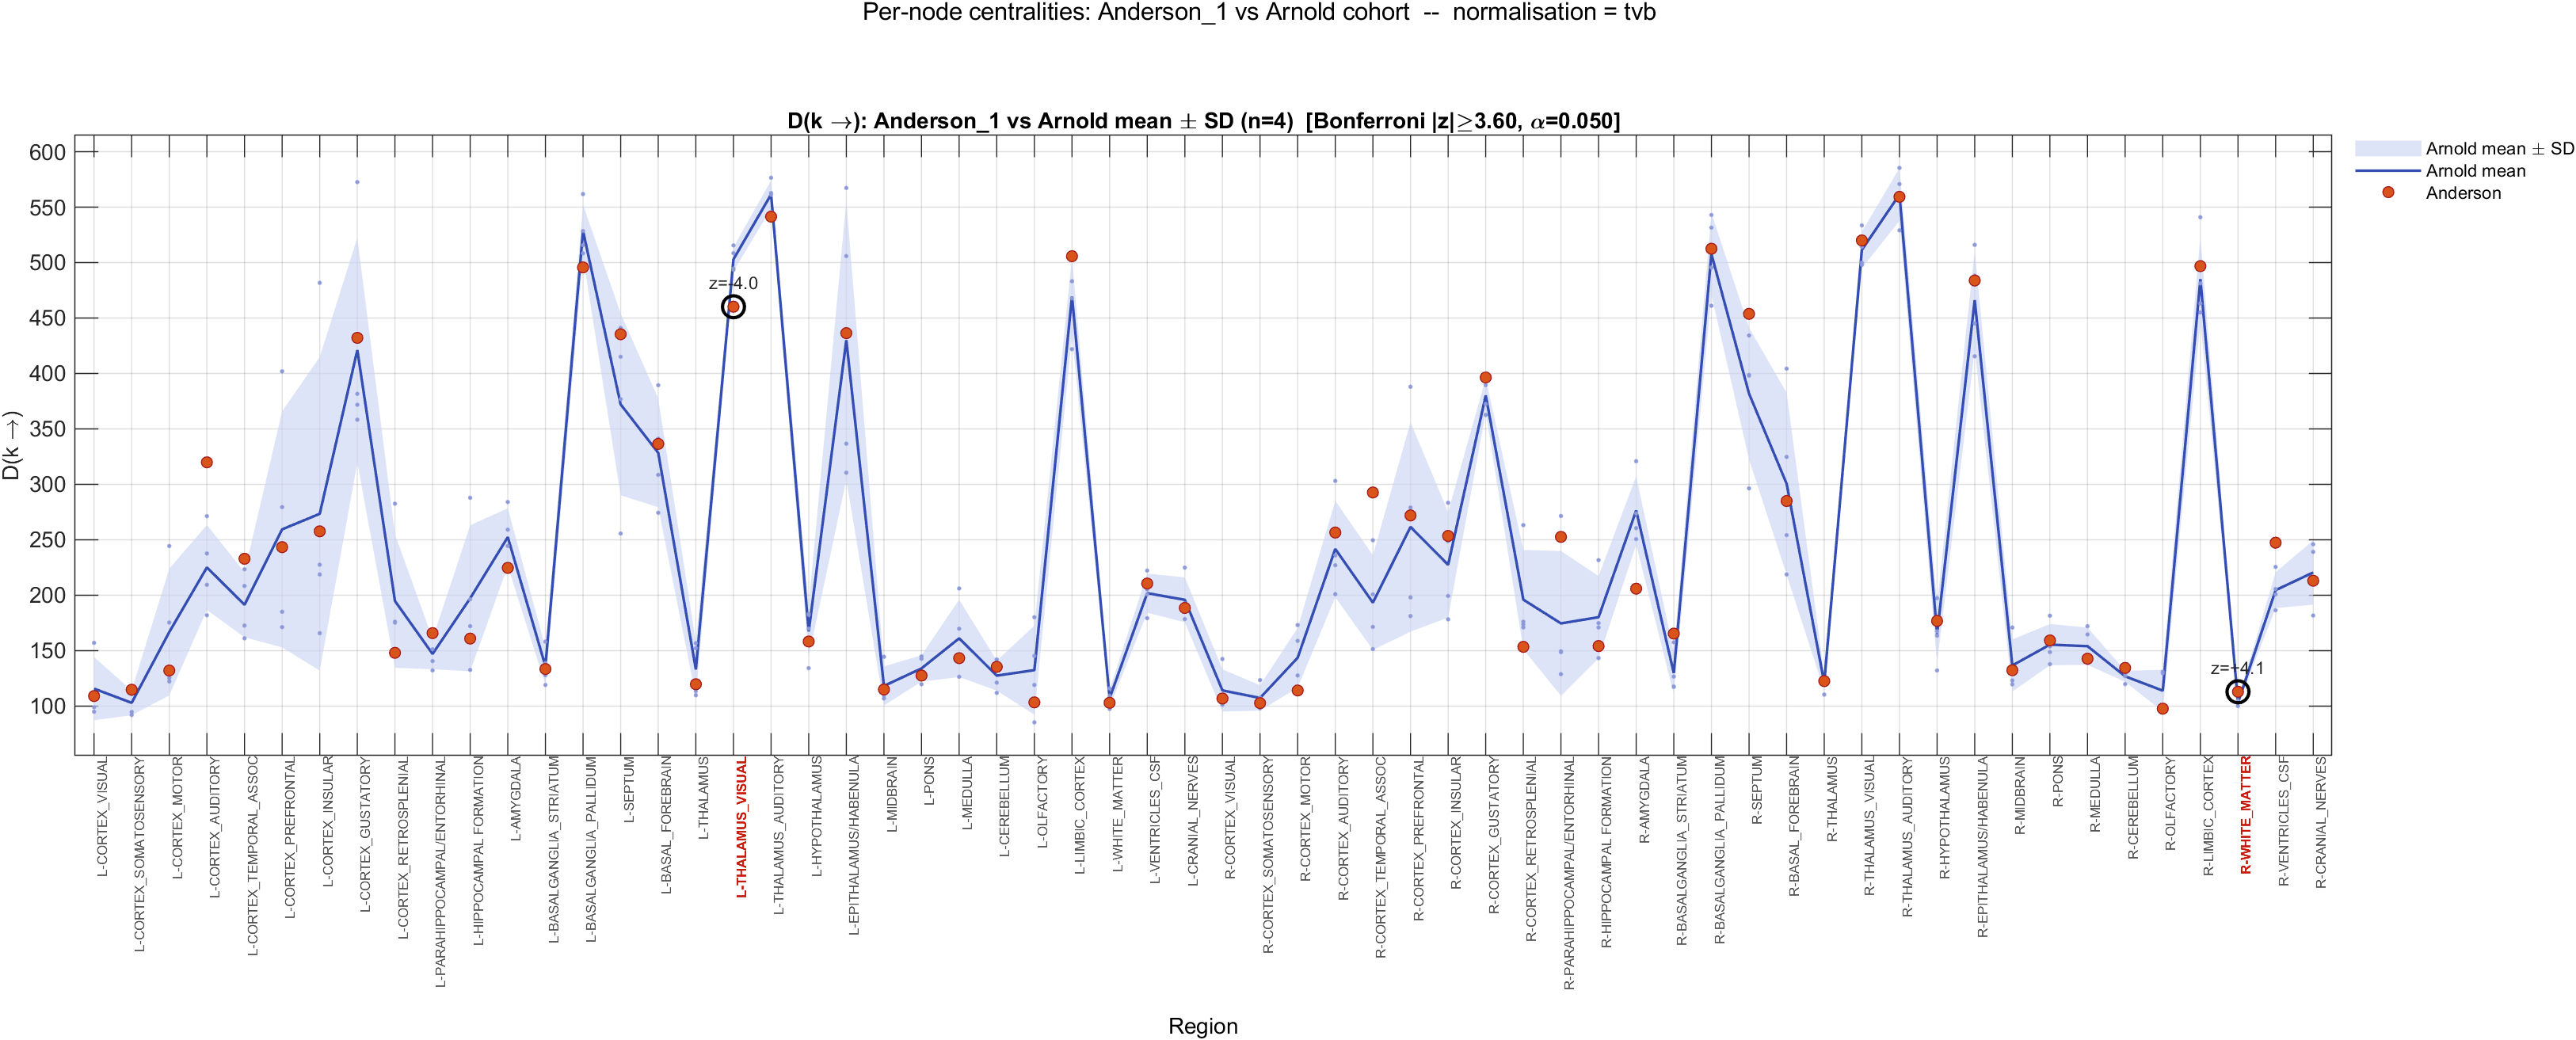
\includegraphics[width=\linewidth]{appendix/compare_anderson_vs_arnold_Anderson_1_tvb_D_k_to.png}
\caption{\textsc{Anderson\_1}, $\Dfrom$}
\end{subfigure}\hfill
\begin{subfigure}{0.32\textwidth}\centering
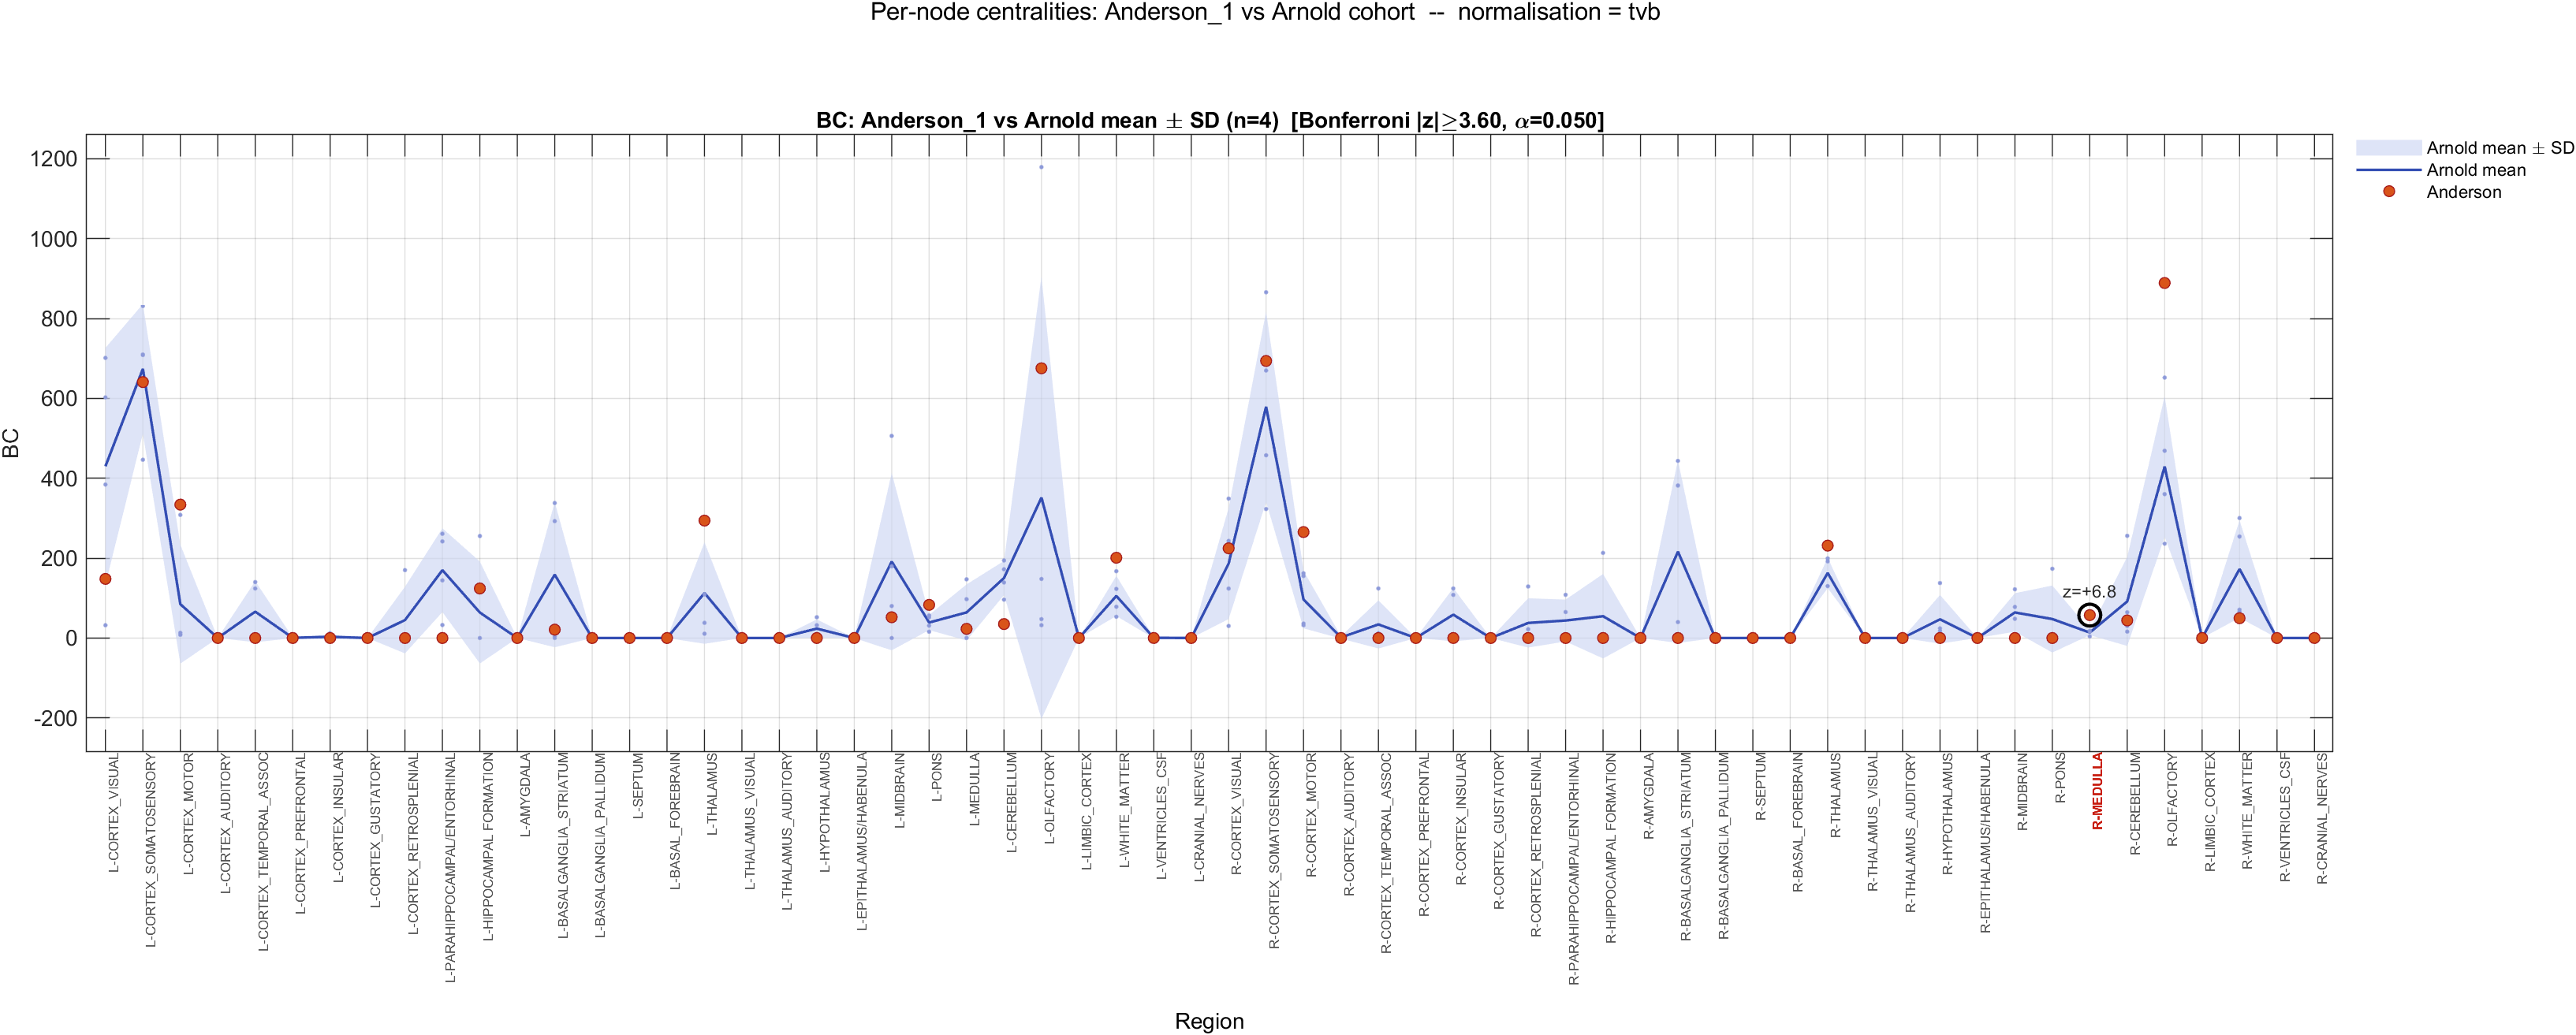
\includegraphics[width=\linewidth]{appendix/compare_anderson_vs_arnold_Anderson_1_tvb_BC.png}
\caption{\textsc{Anderson\_1}, BC}
\end{subfigure}\hfill
\begin{subfigure}{0.32\textwidth}\centering
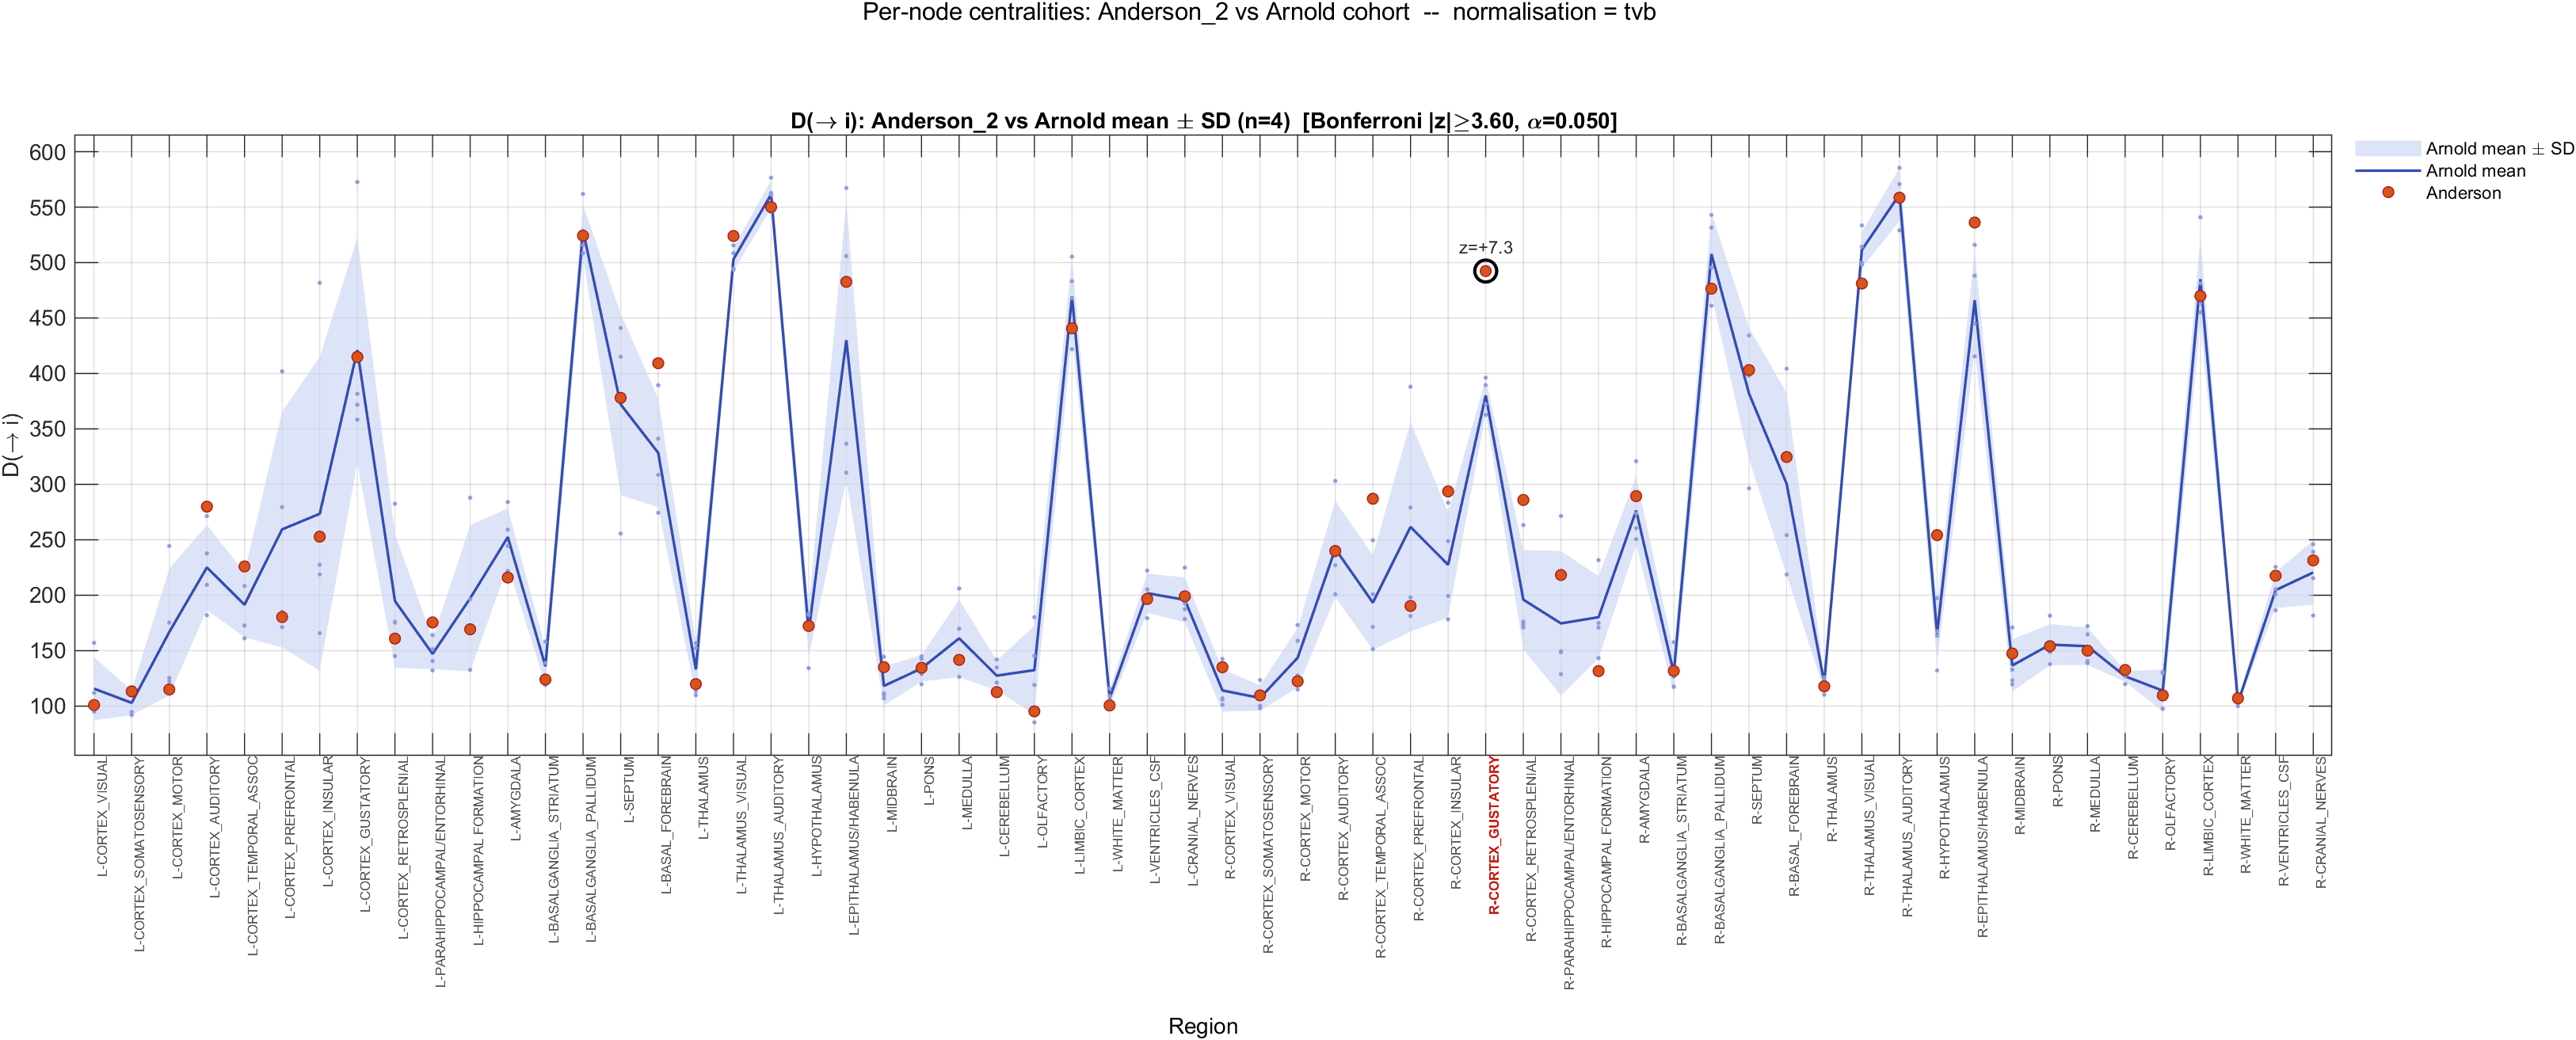
\includegraphics[width=\linewidth]{appendix/compare_anderson_vs_arnold_Anderson_2_tvb_D_to_i.png}
\caption{\textsc{Anderson\_2}, $\Dto$}
\end{subfigure}\hfill
\begin{subfigure}{0.32\textwidth}\centering
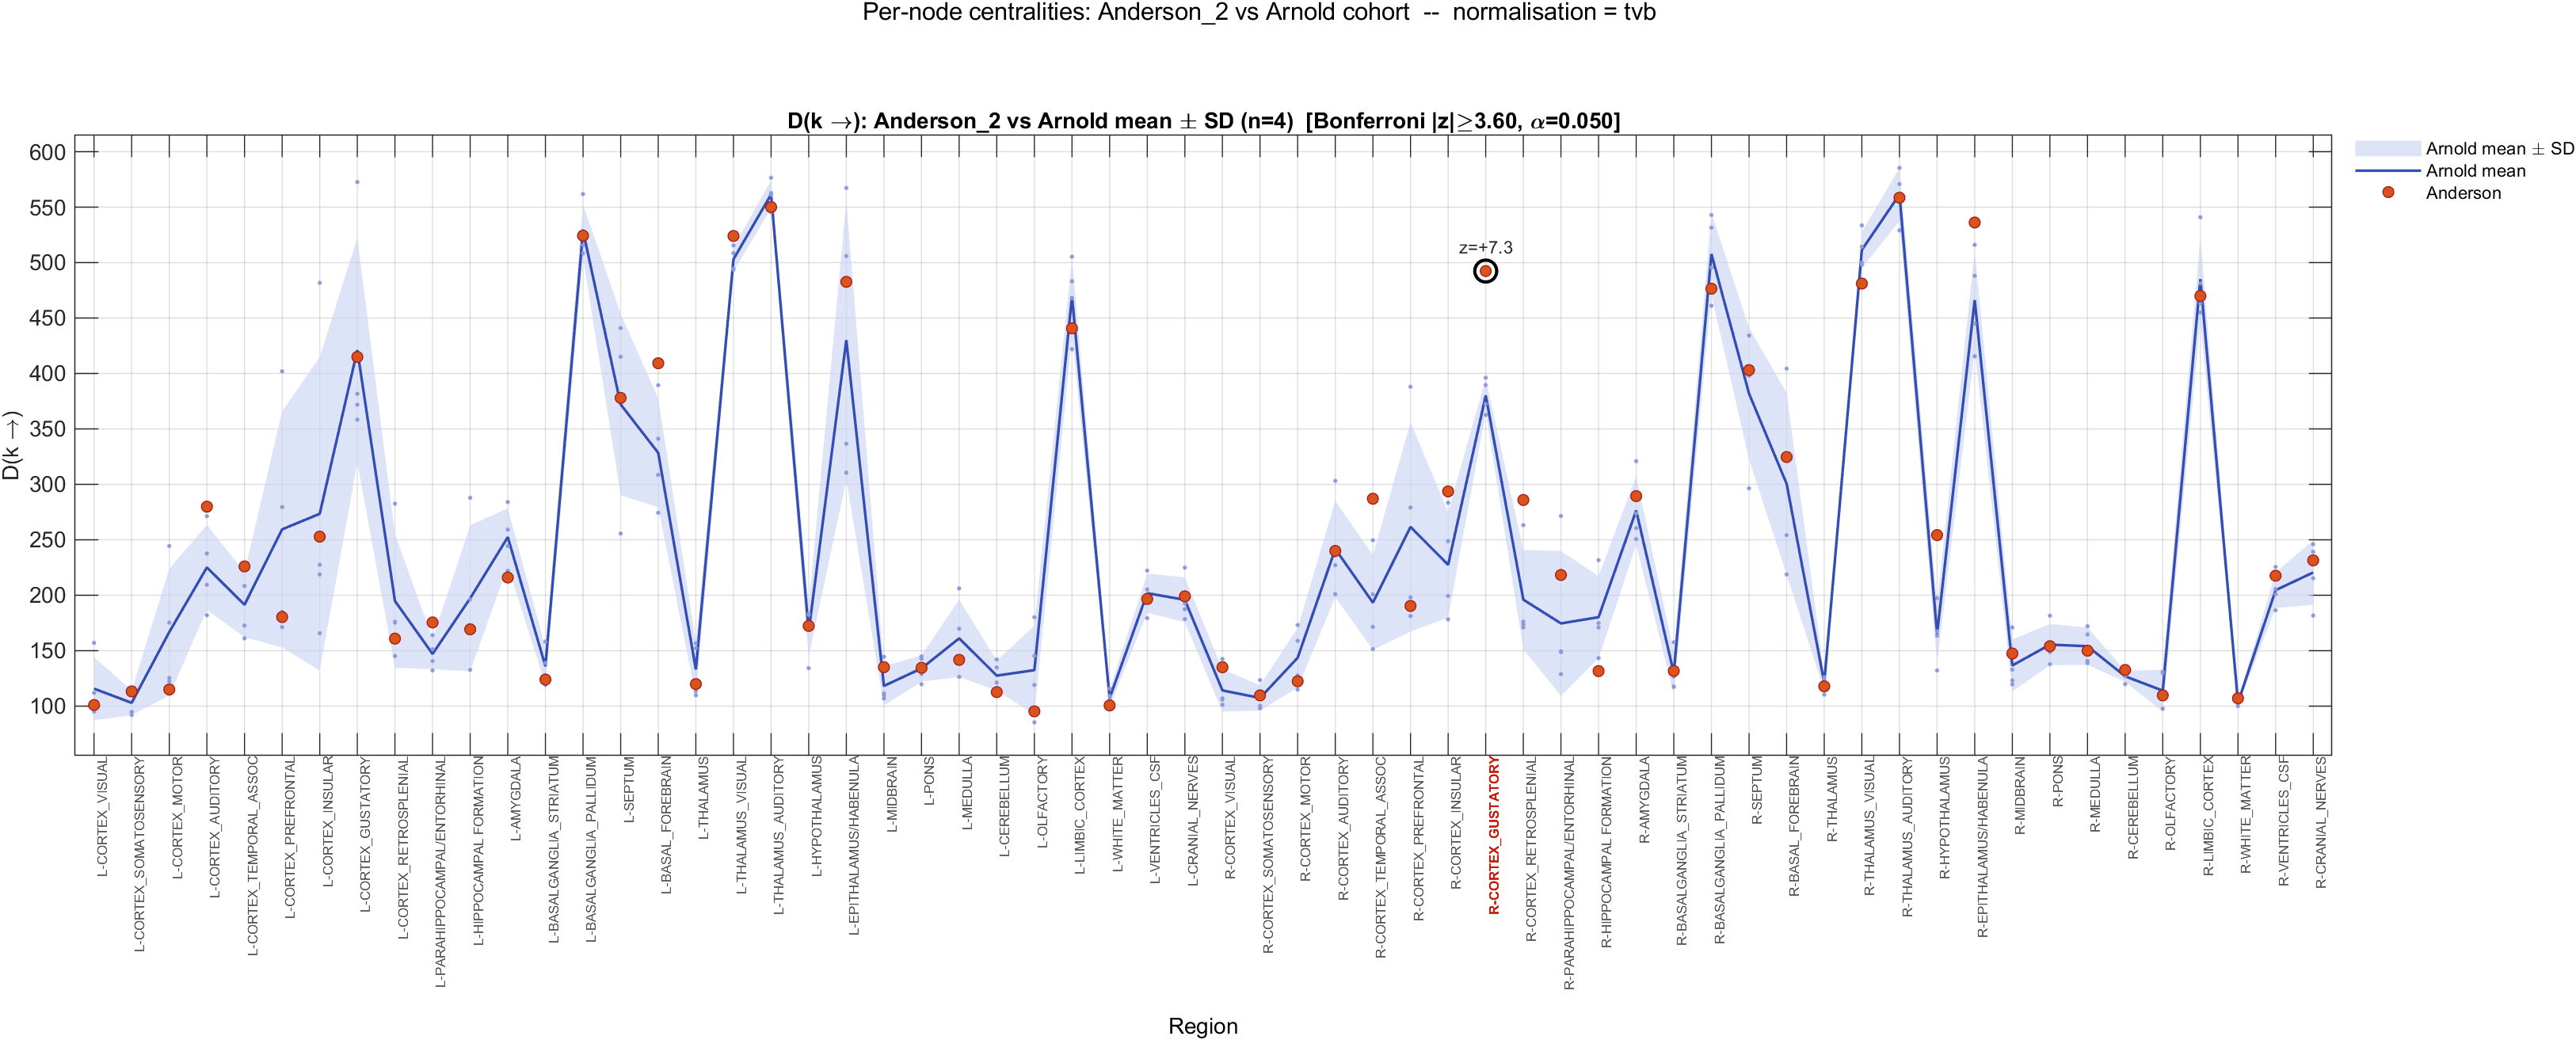
\includegraphics[width=\linewidth]{appendix/compare_anderson_vs_arnold_Anderson_2_tvb_D_k_to.png}
\caption{\textsc{Anderson\_2}, $\Dfrom$}
\end{subfigure}\hfill
\begin{subfigure}{0.32\textwidth}\centering
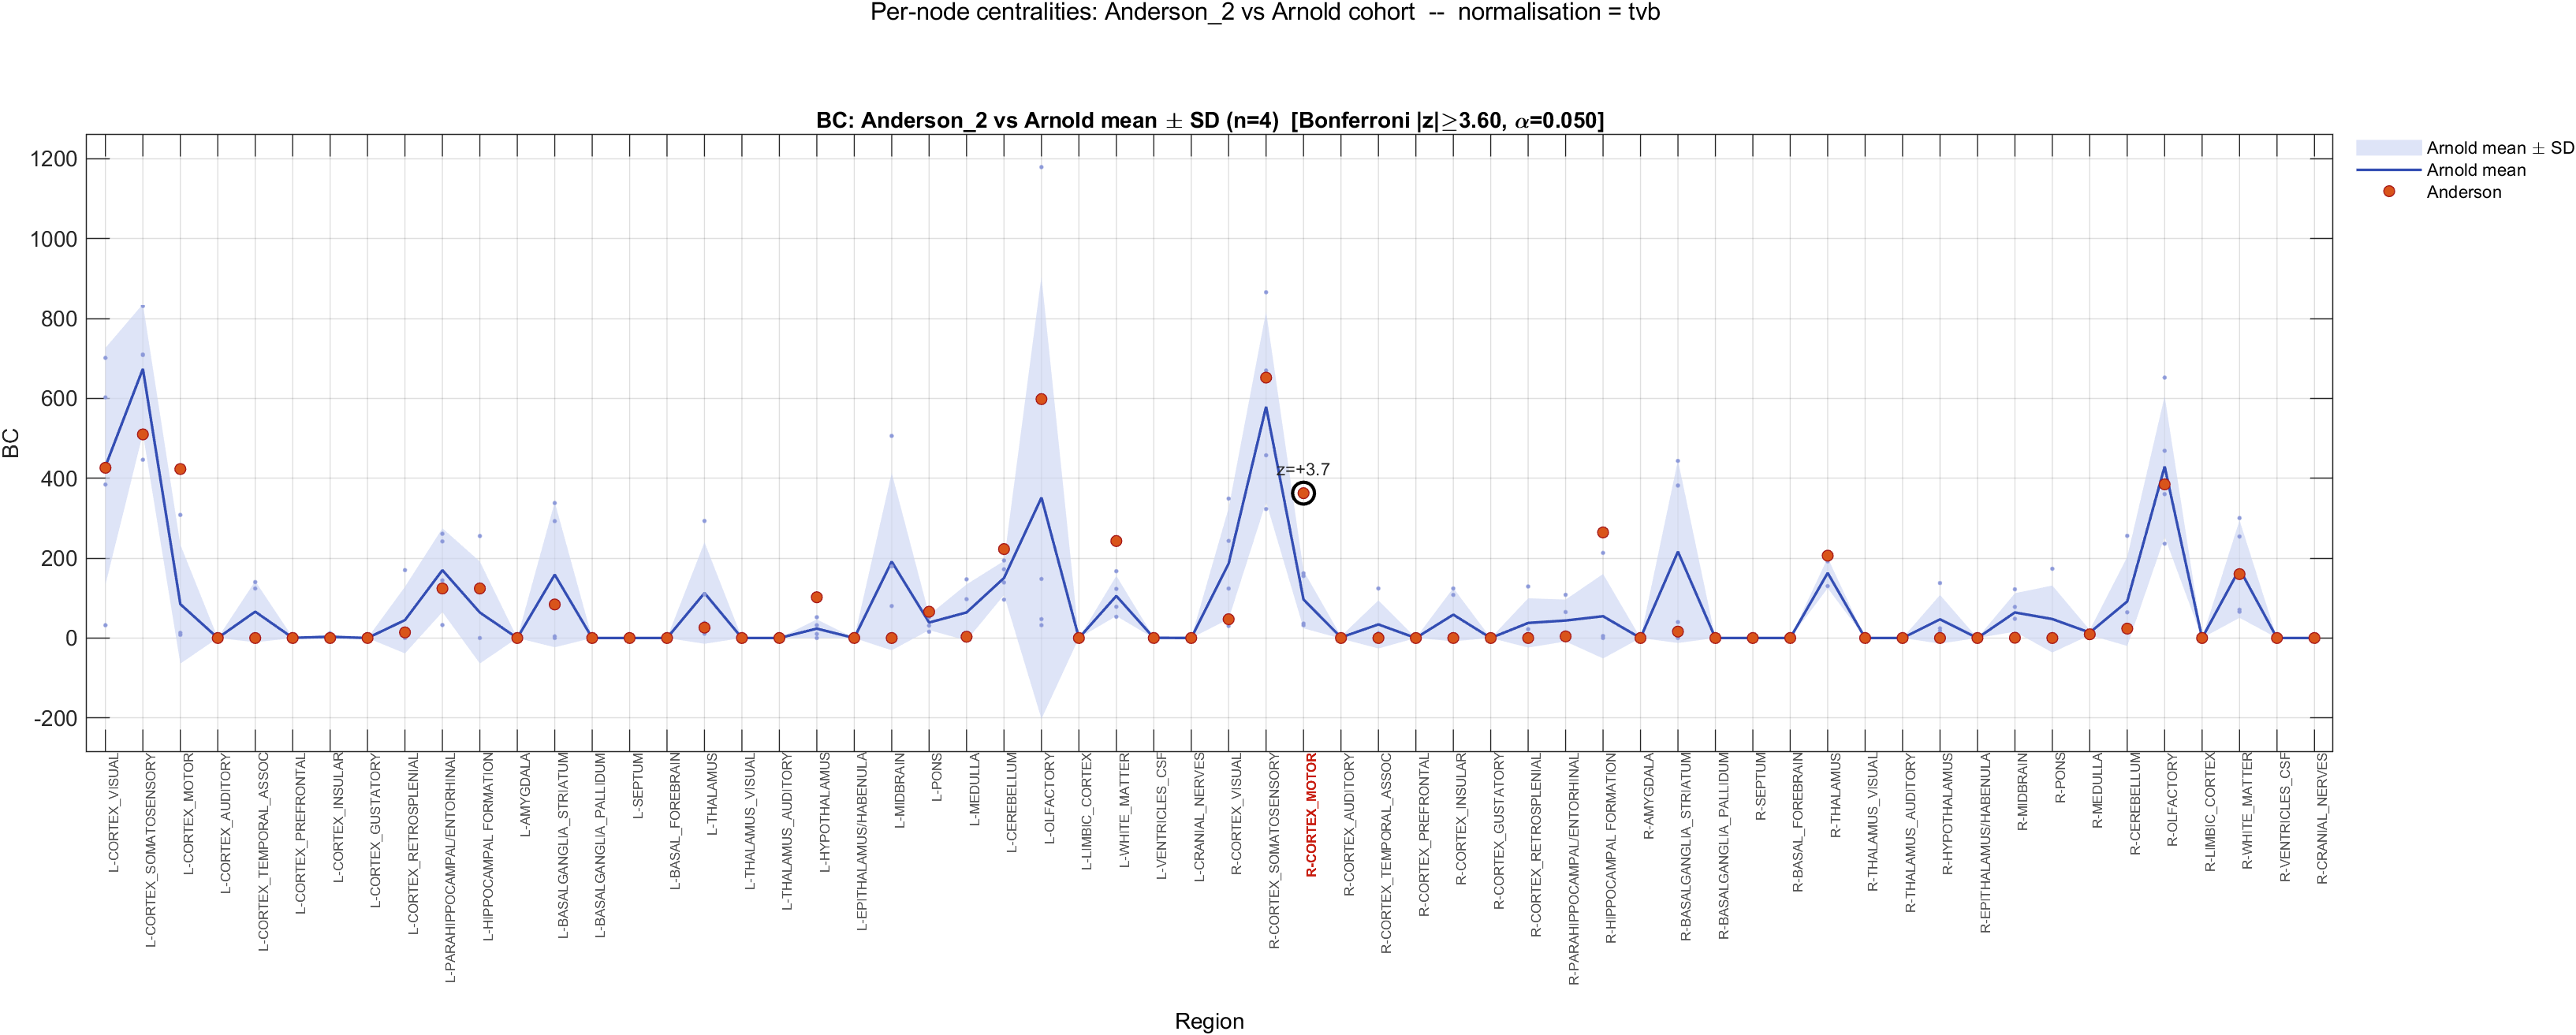
\includegraphics[width=\linewidth]{appendix/compare_anderson_vs_arnold_Anderson_2_tvb_BC.png}
\caption{\textsc{Anderson\_2}, BC}
\end{subfigure}\hfill
\caption{Each case mouse against the four-control band, \texttt{tvb} scheme: susceptibility $\Dto$, influence $\Dfrom$, and betweenness BC.}
\end{figure}

\subsection{Left--right asymmetry}
\begin{figure}[H]\centering
\begin{subfigure}{0.46\textwidth}\centering
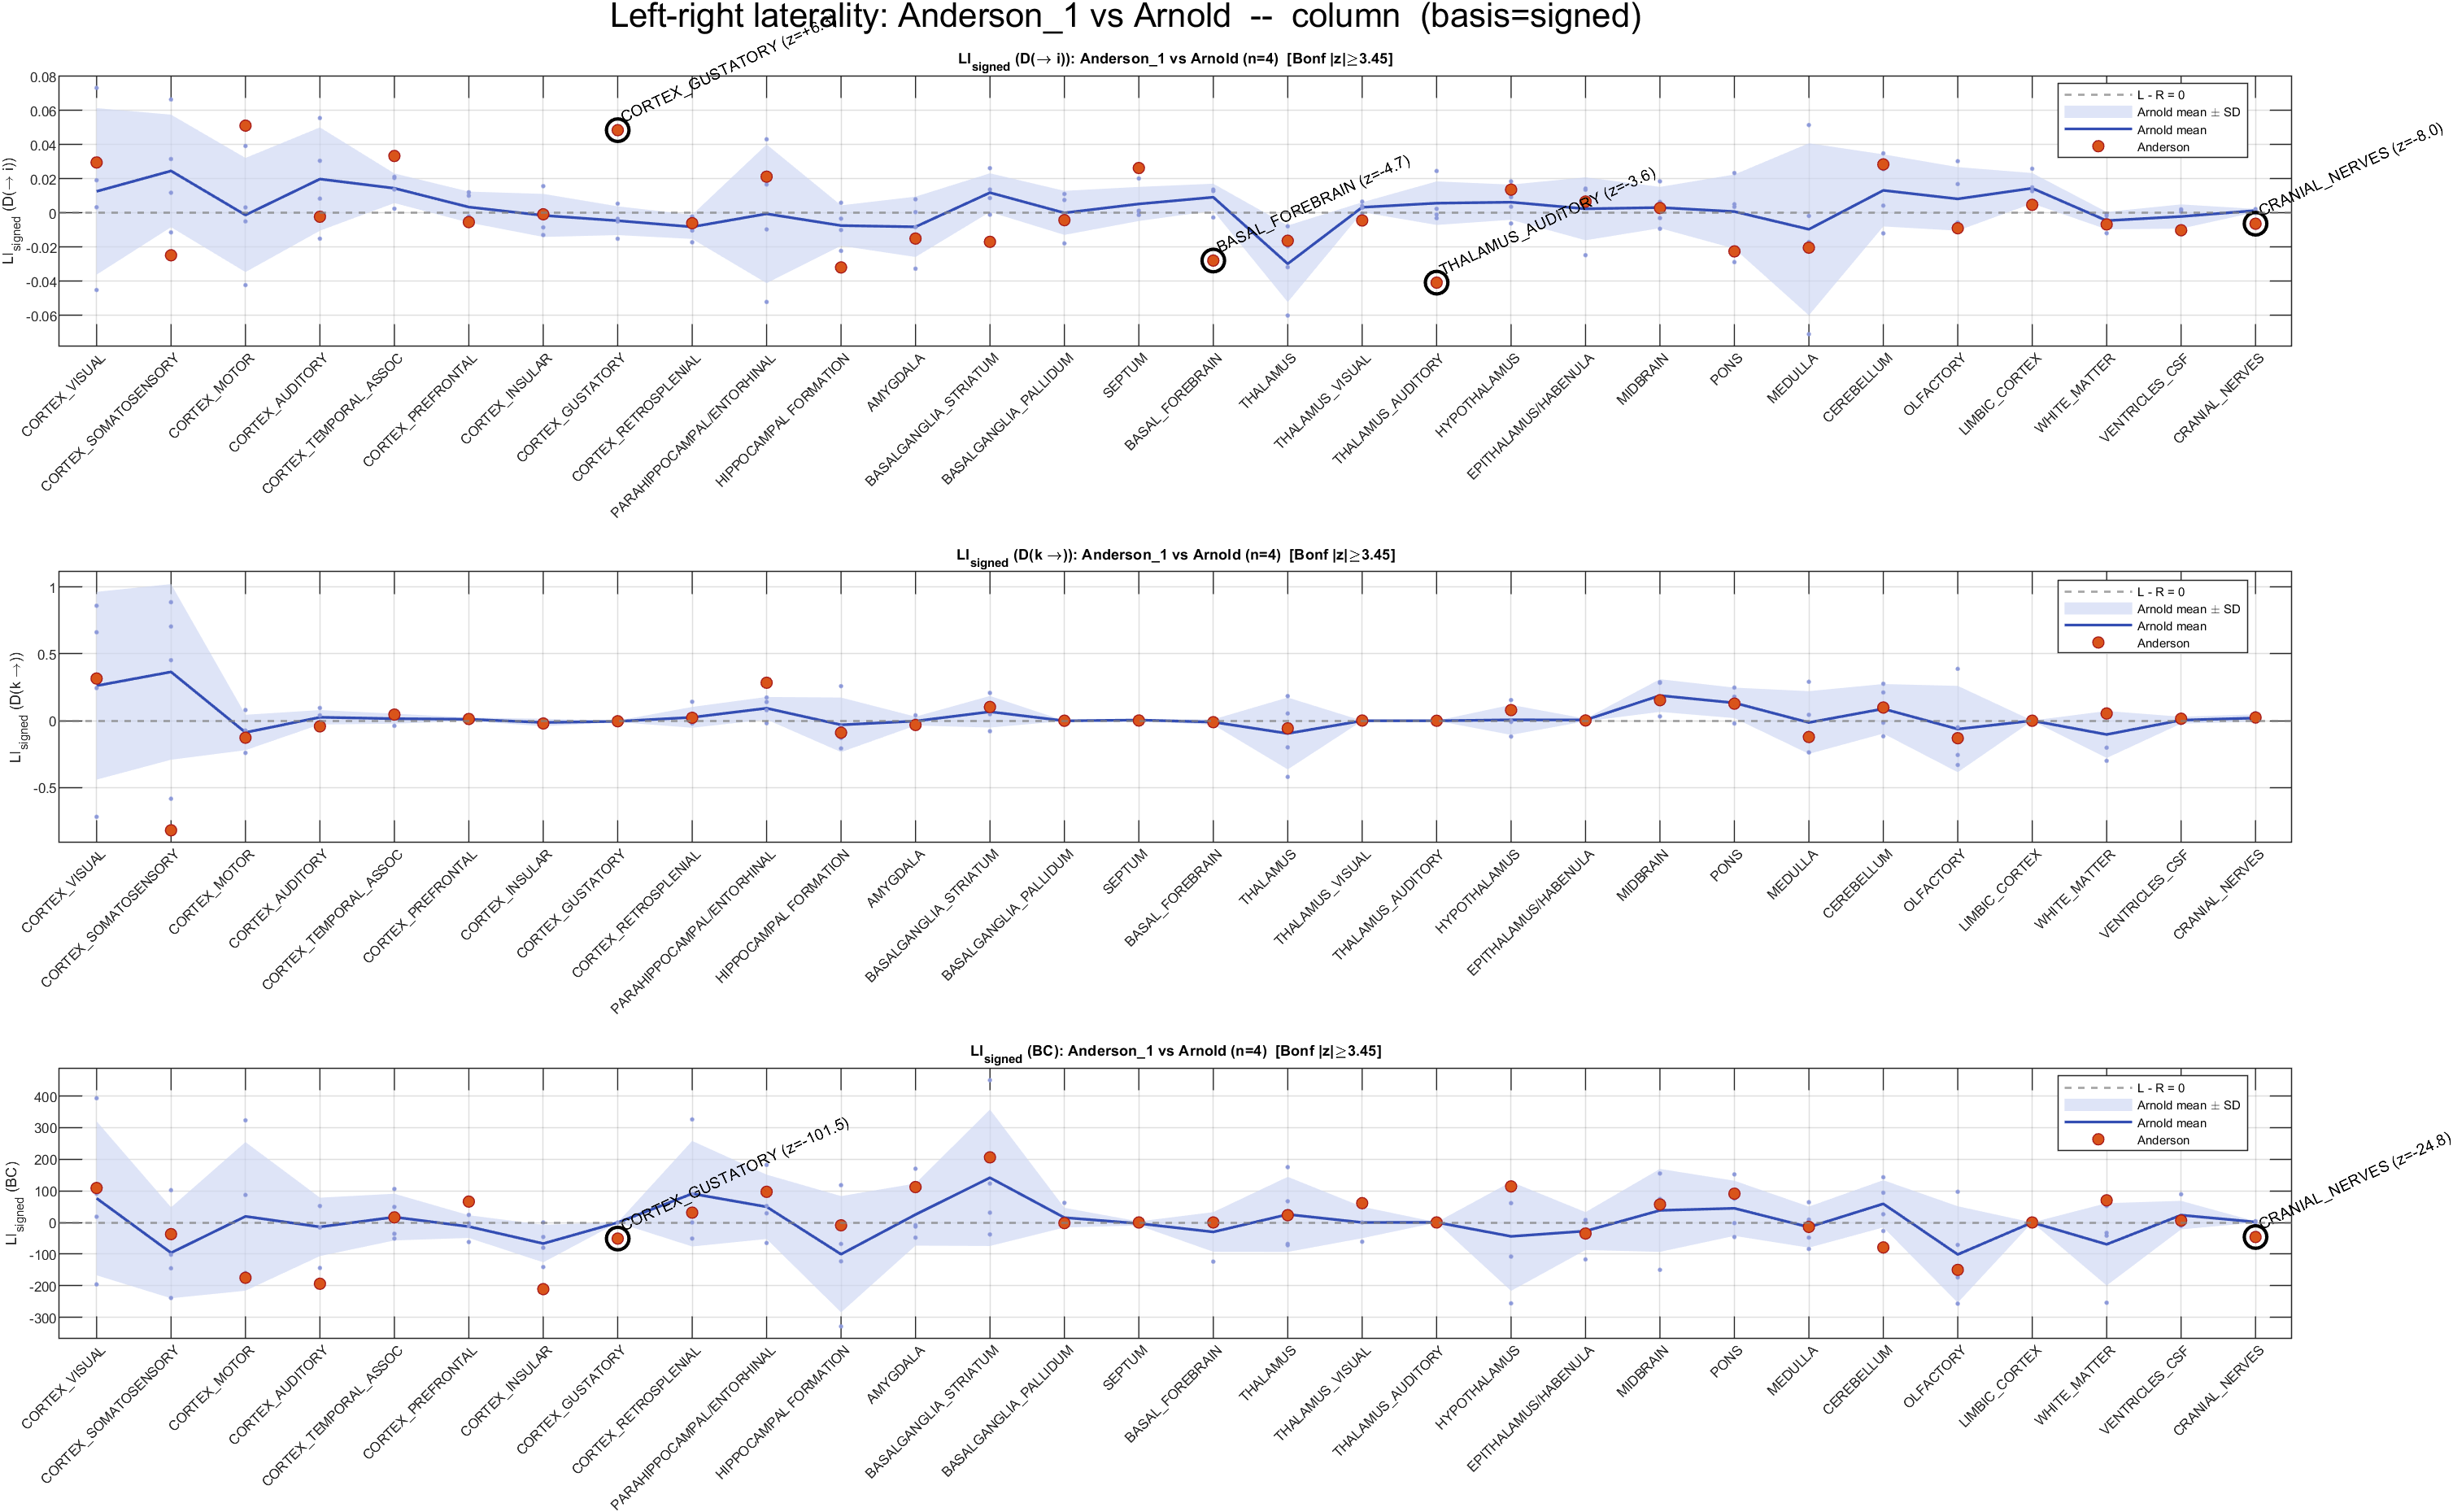
\includegraphics[width=\linewidth]{appendix/compare_LR_asymmetry_Anderson_1_column.png}
\caption{\textsc{Anderson\_1}}
\end{subfigure}\hfill
\begin{subfigure}{0.46\textwidth}\centering
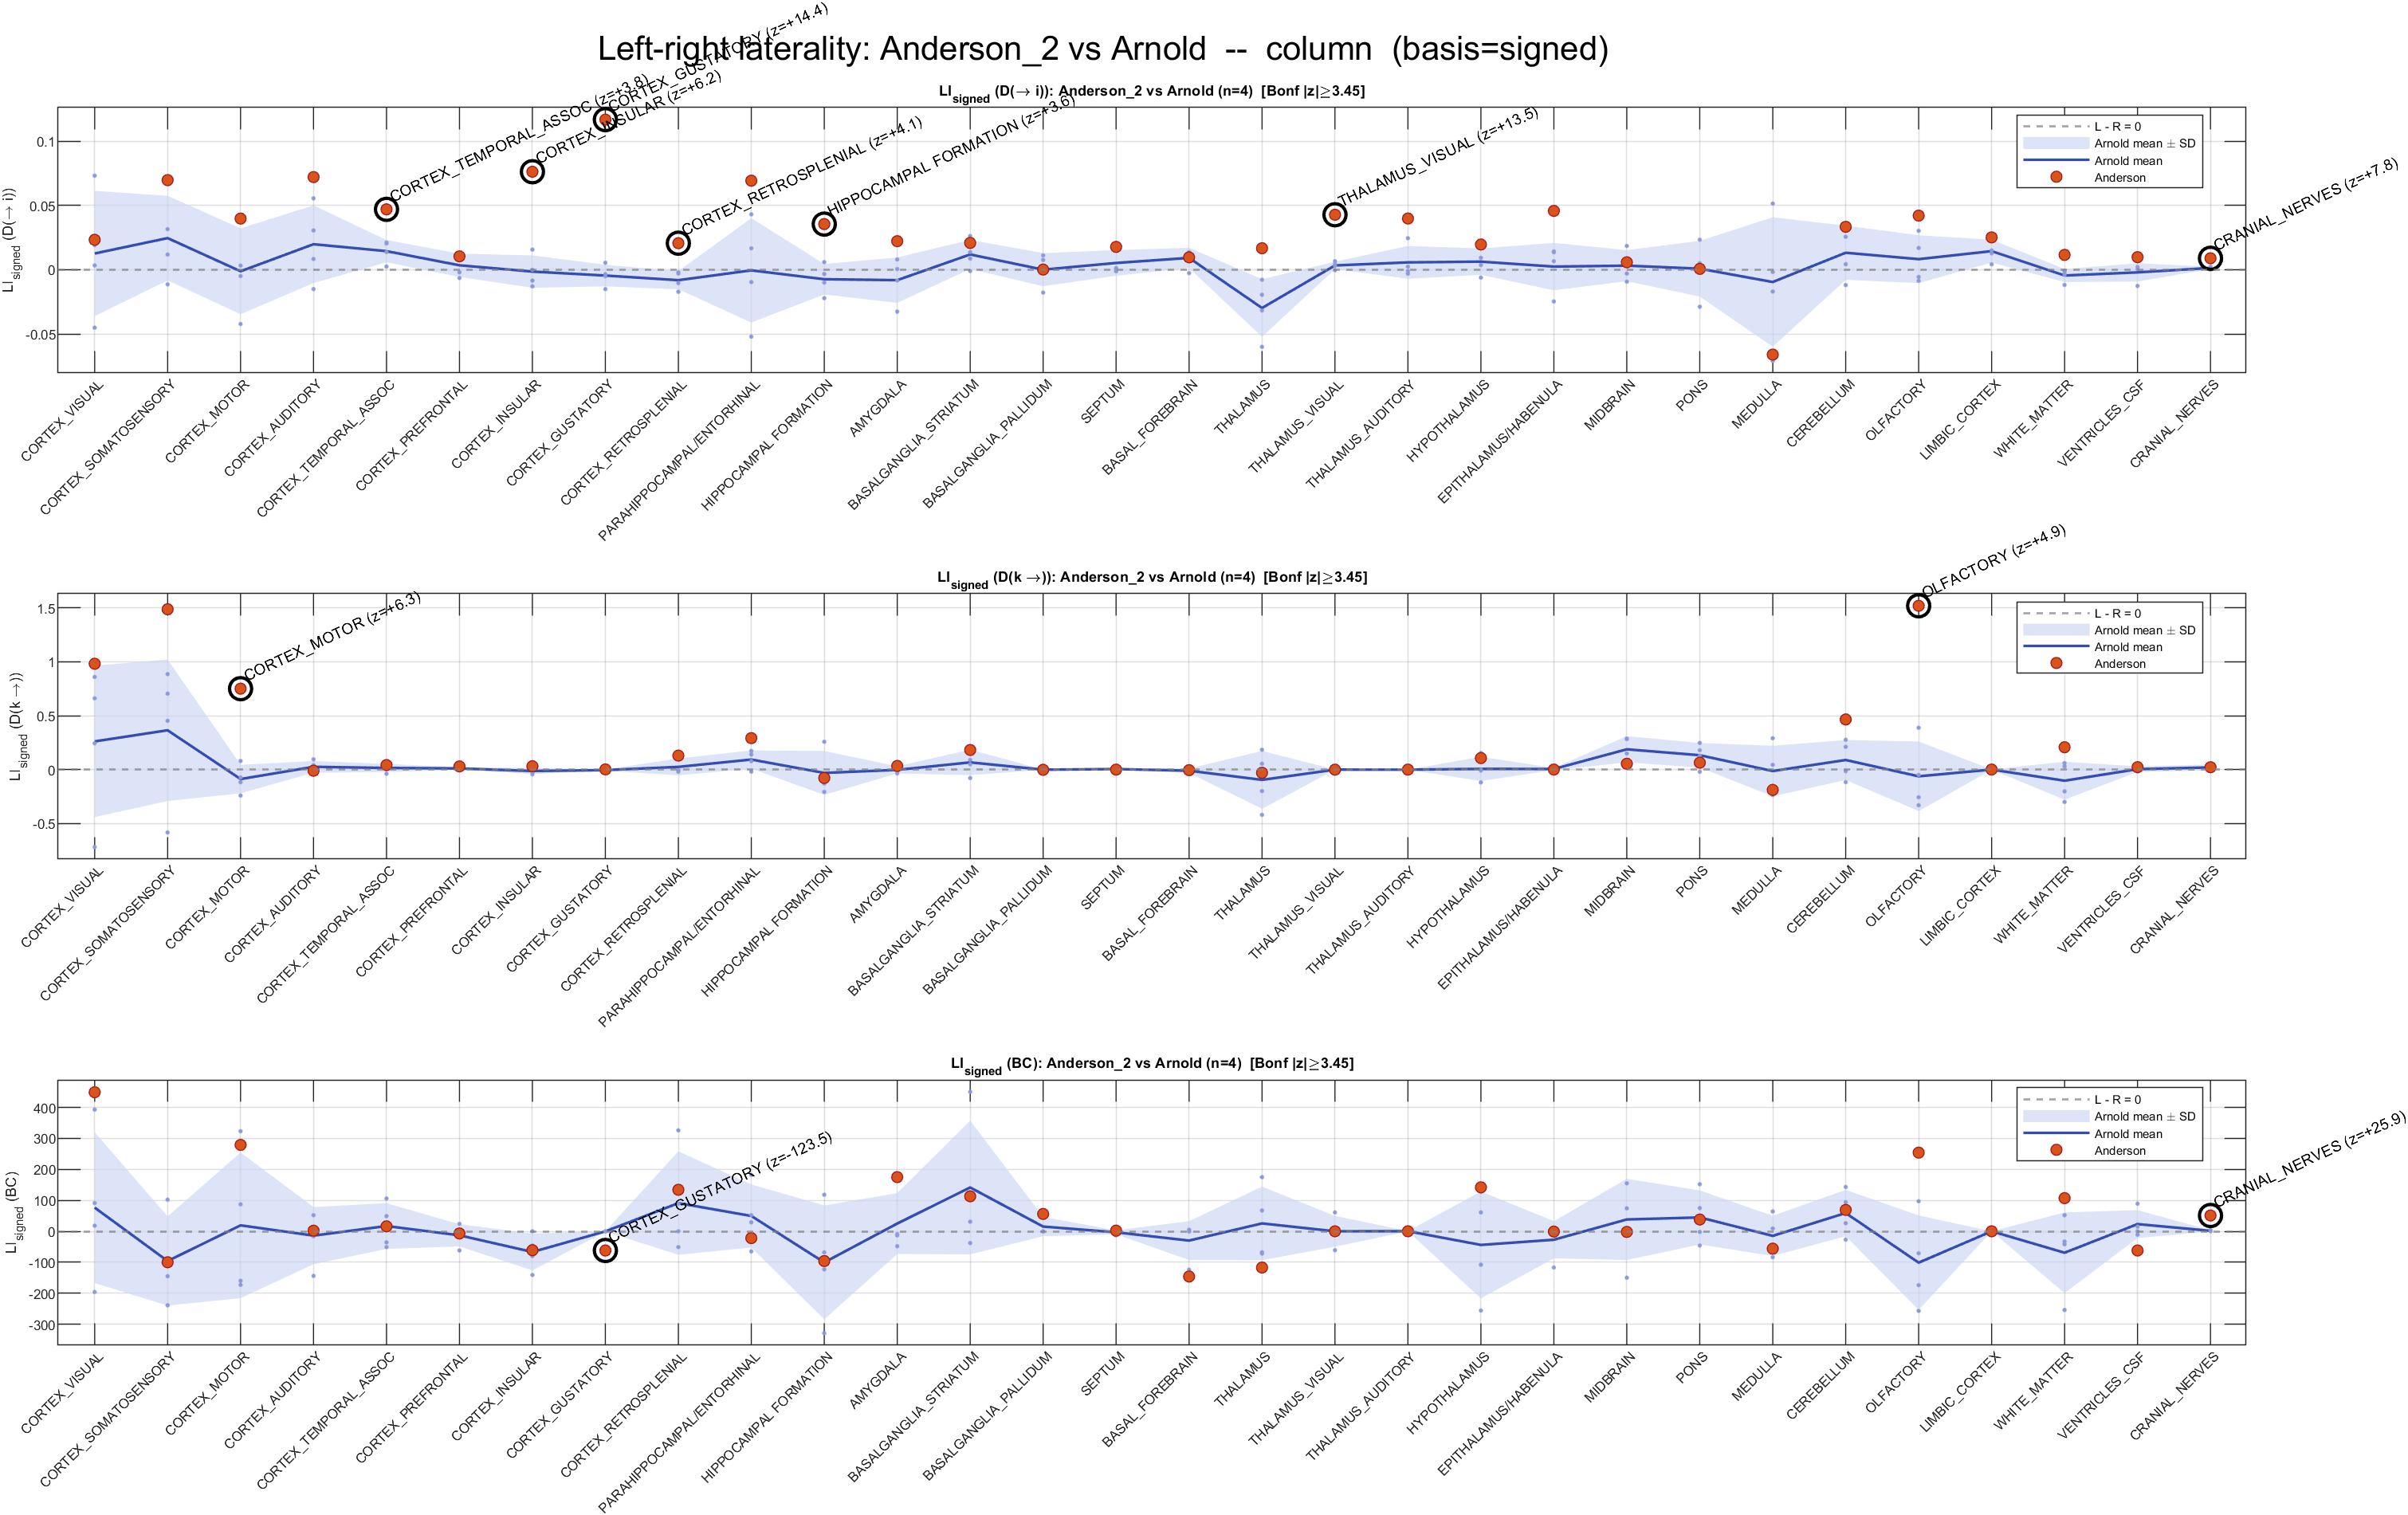
\includegraphics[width=\linewidth]{appendix/compare_LR_asymmetry_Anderson_2_column.png}
\caption{\textsc{Anderson\_2}}
\end{subfigure}\hfill
\begin{subfigure}{0.46\textwidth}\centering
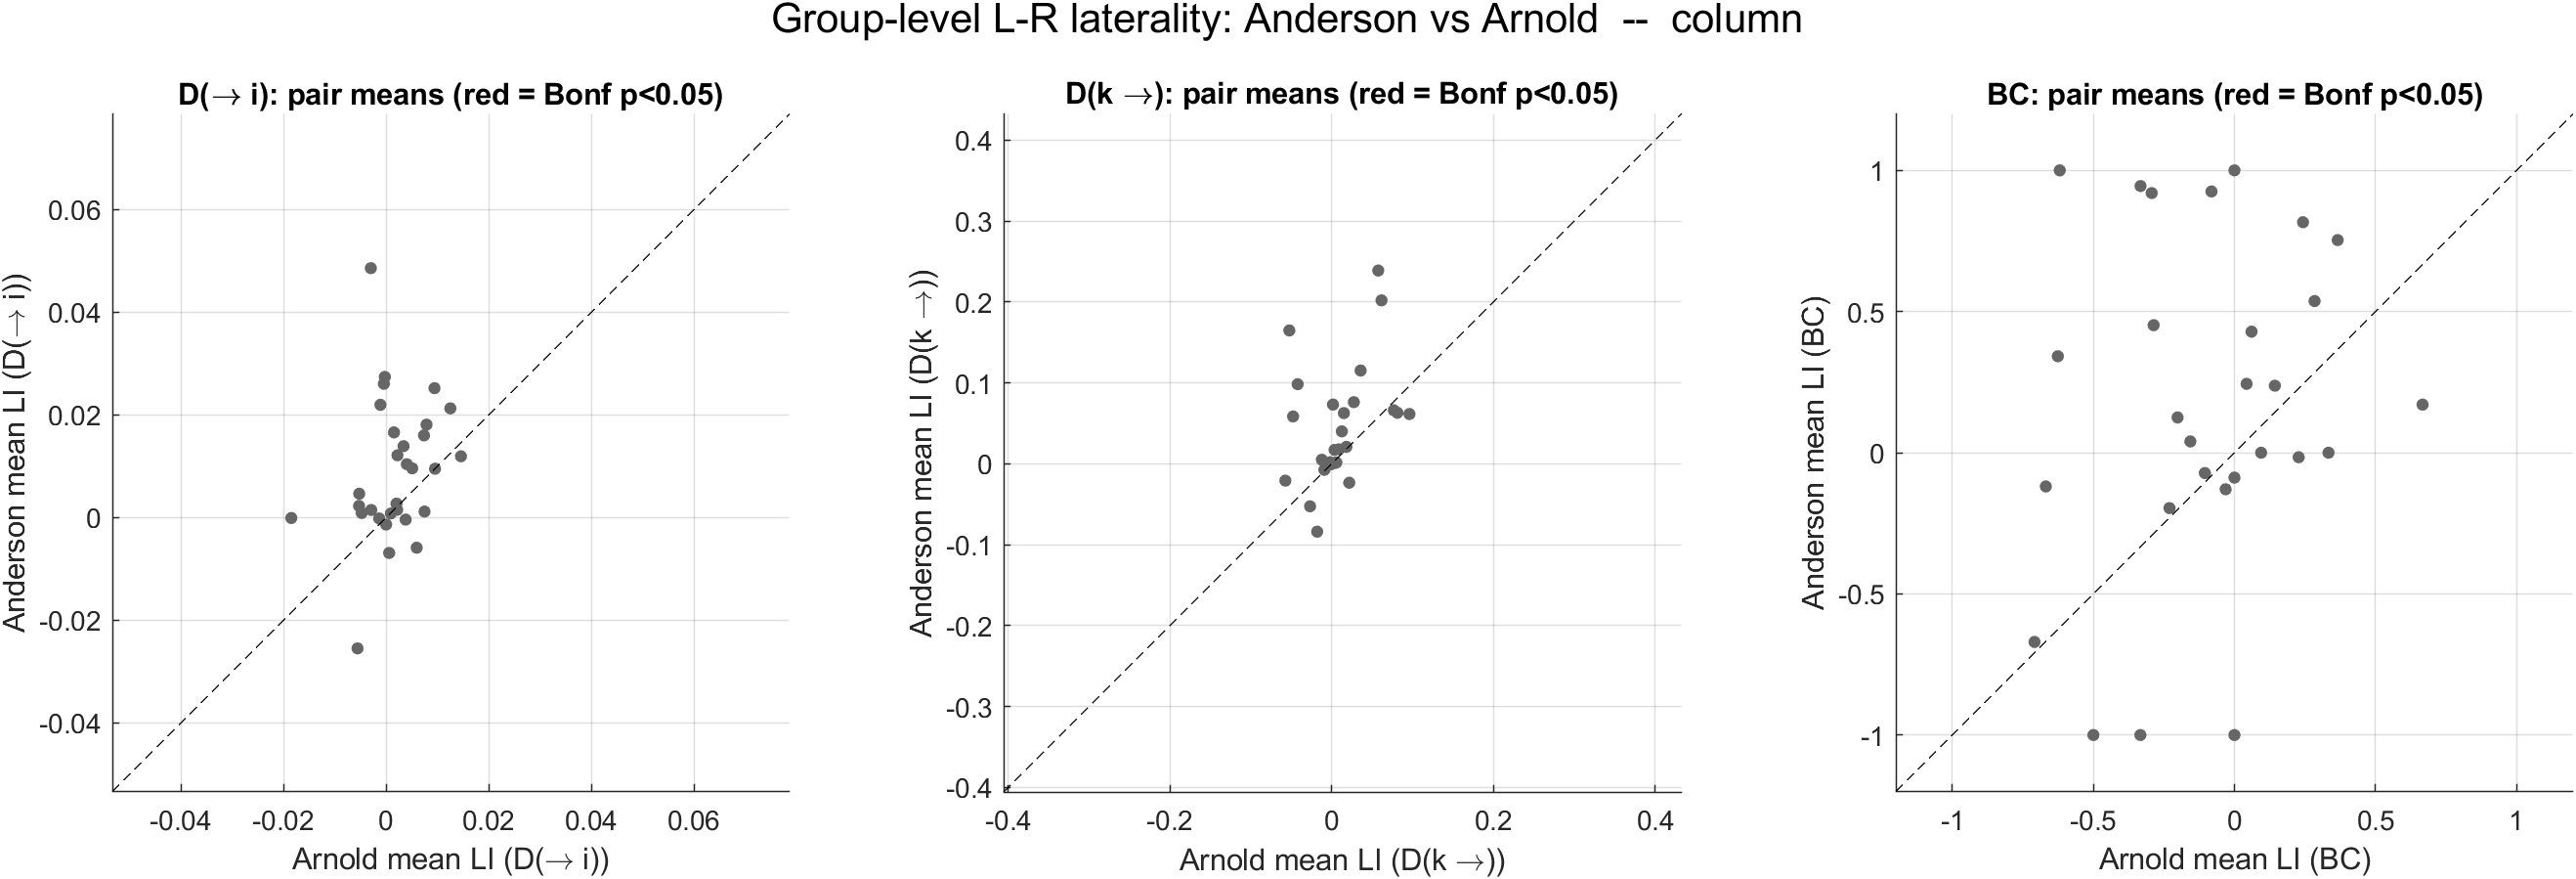
\includegraphics[width=\linewidth]{appendix/LR_asymmetry_groupTest_column.png}
\caption{Homotopic-pair group test}
\end{subfigure}\hfill
\begin{subfigure}{0.46\textwidth}\centering
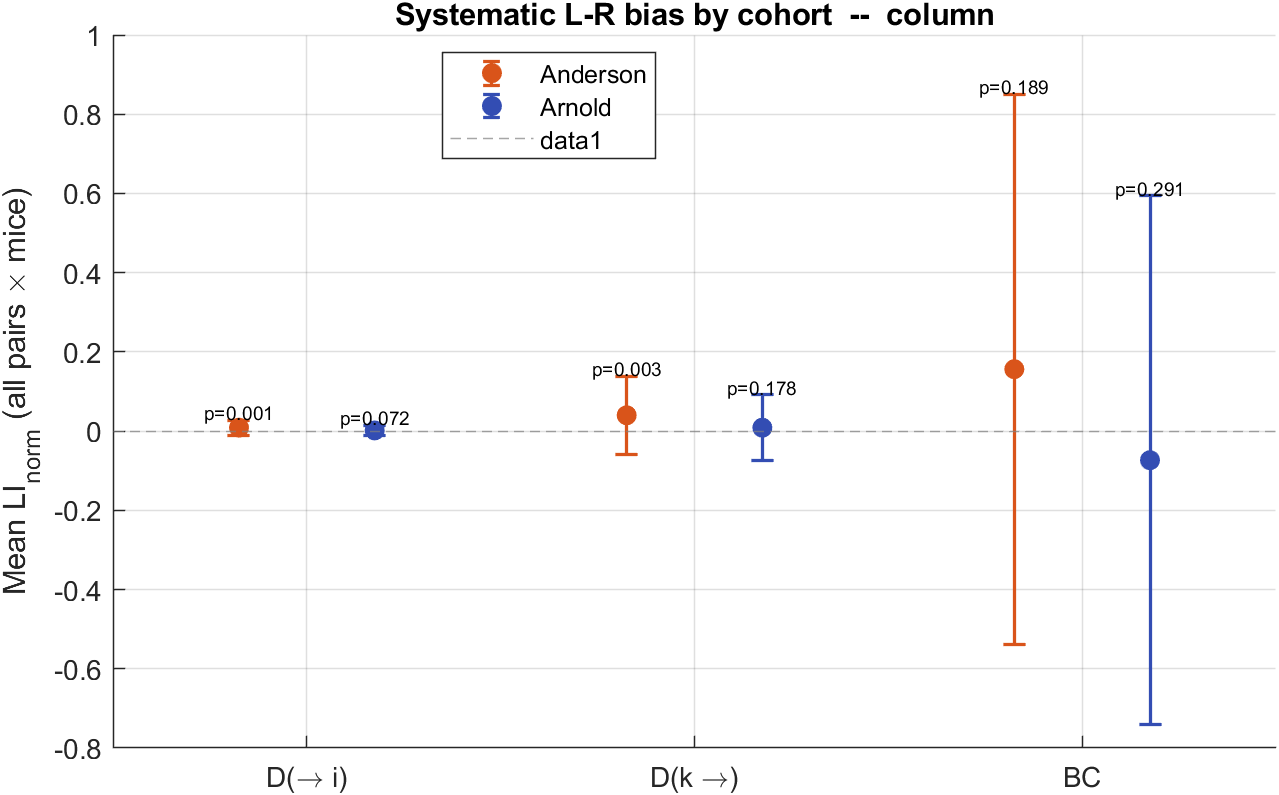
\includegraphics[width=\linewidth]{appendix/LR_asymmetry_systematic_column.png}
\caption{Systematic side bias}
\end{subfigure}
\caption{Left--right asymmetry views, \texttt{column} scheme.}
\end{figure}

\begin{figure}[H]\centering
\begin{subfigure}{0.46\textwidth}\centering
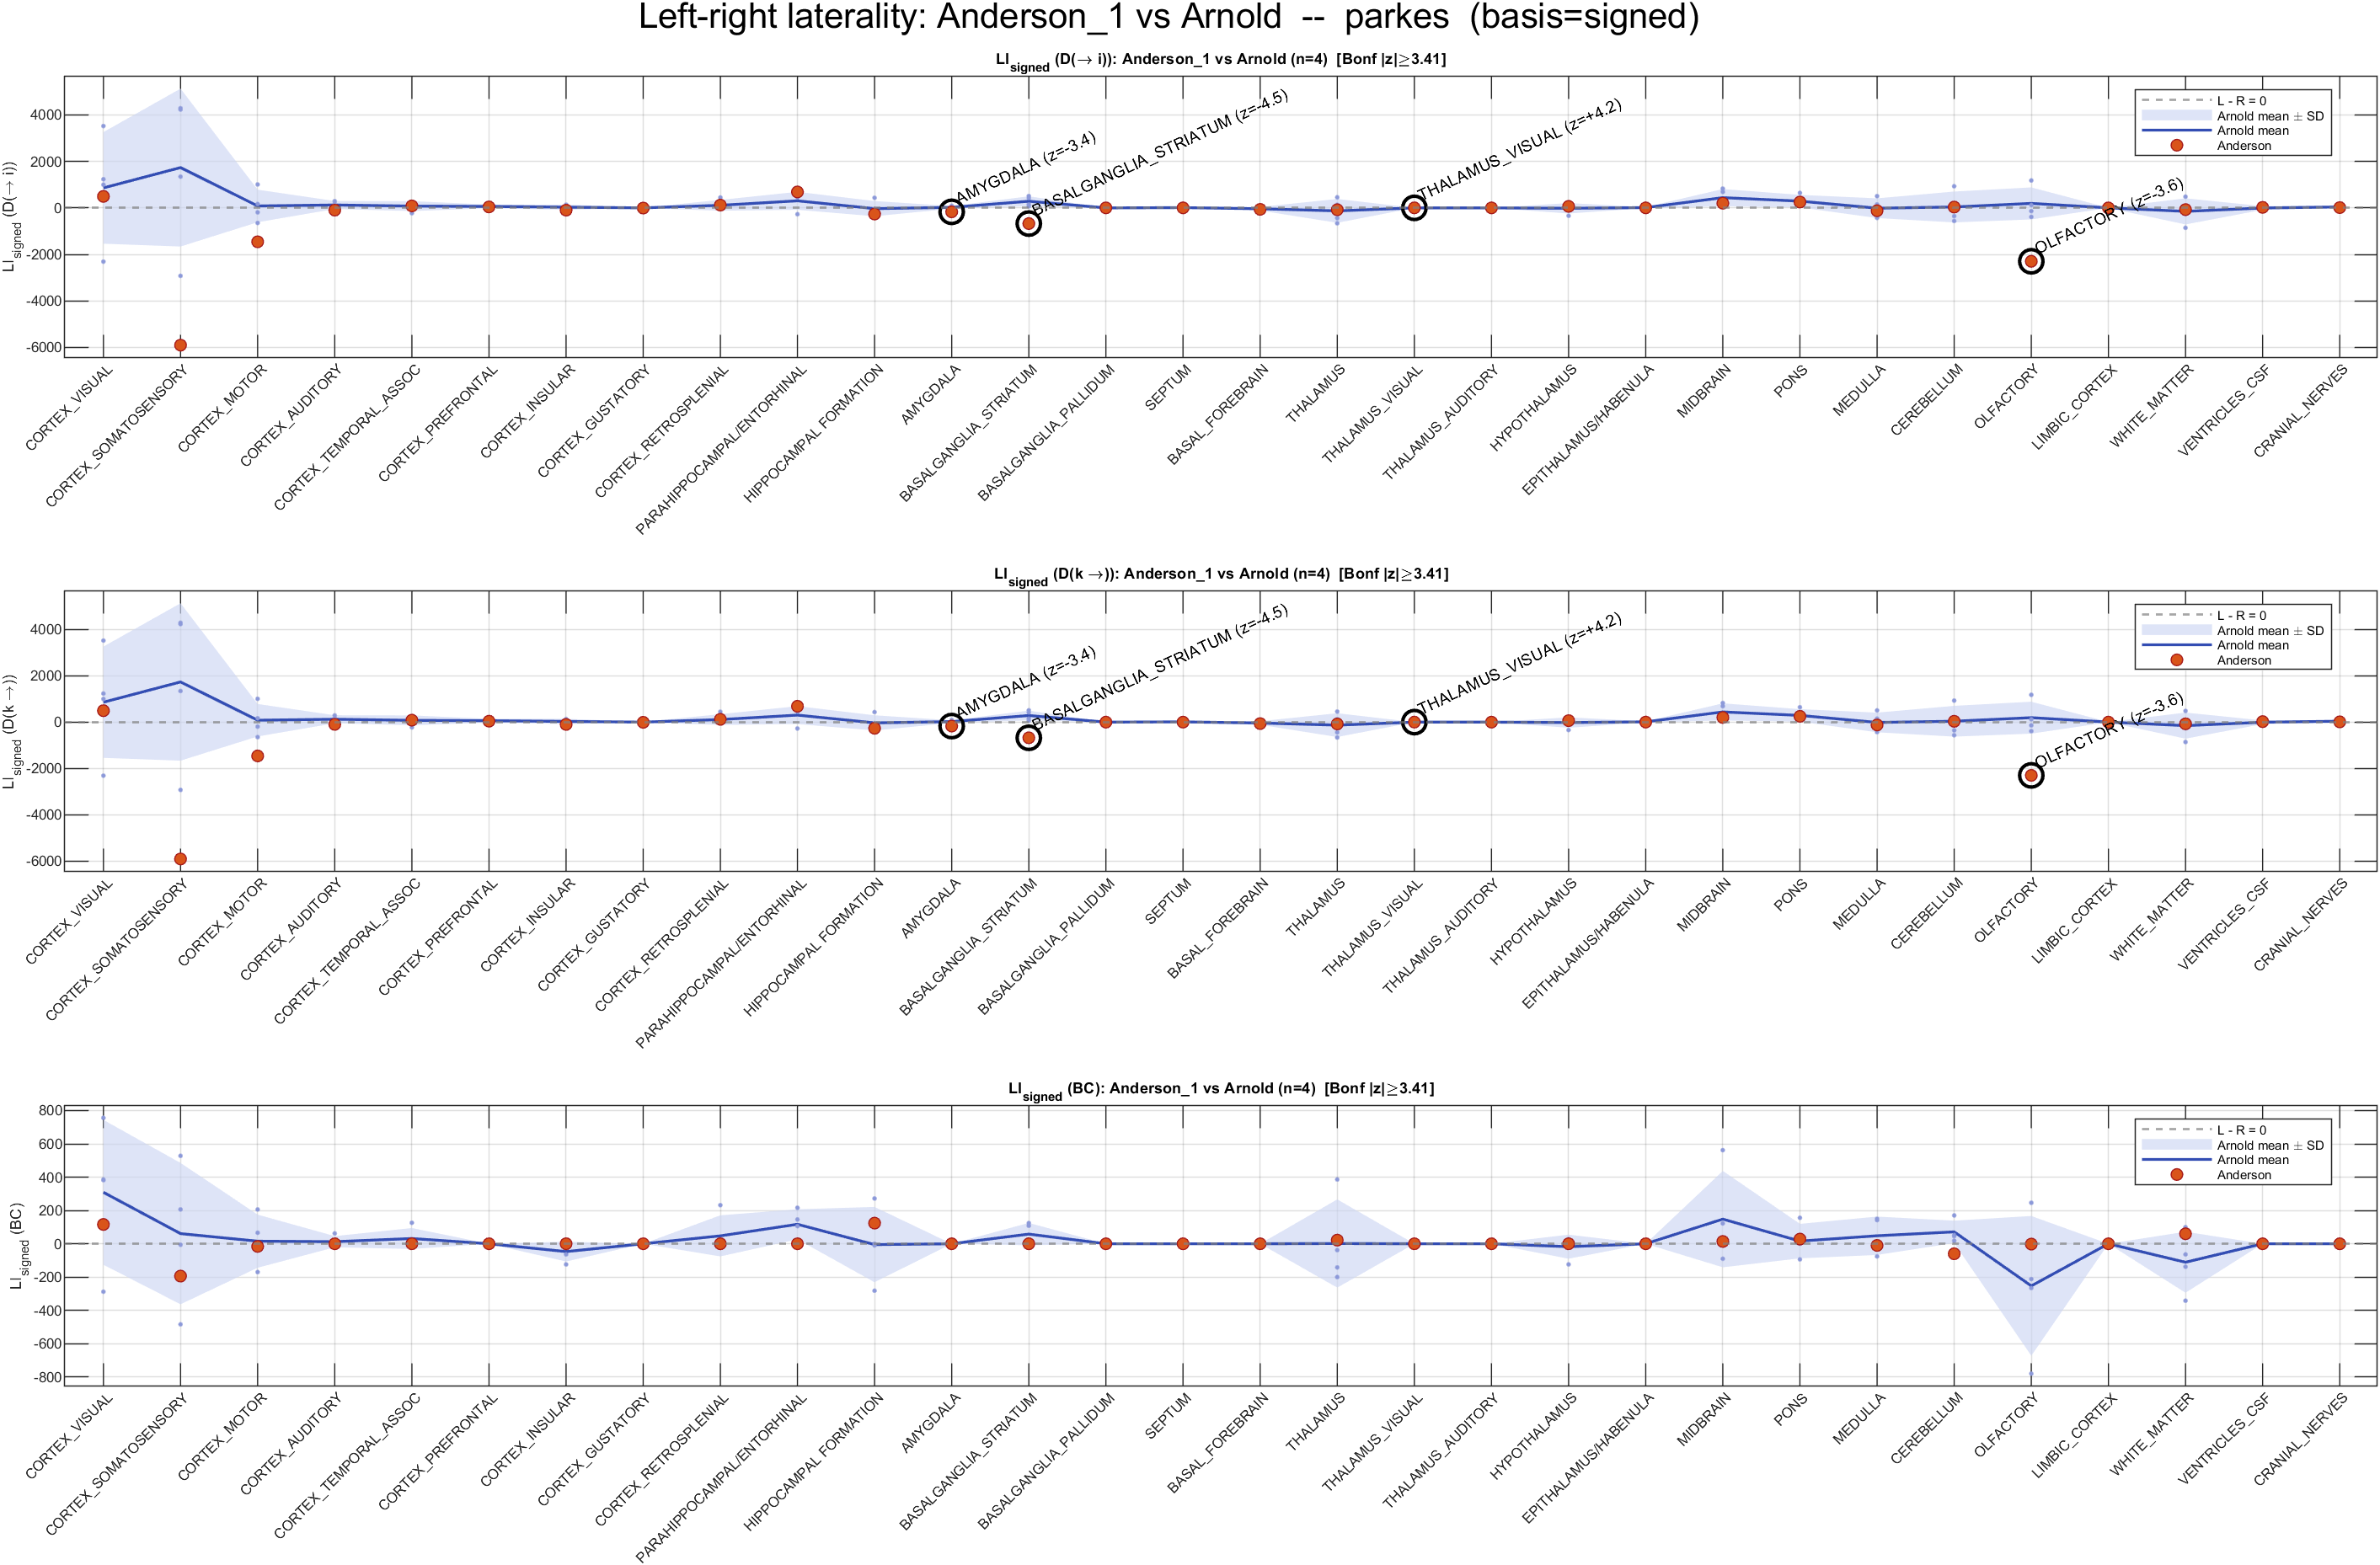
\includegraphics[width=\linewidth]{appendix/compare_LR_asymmetry_Anderson_1_parkes.png}
\caption{\textsc{Anderson\_1}}
\end{subfigure}\hfill
\begin{subfigure}{0.46\textwidth}\centering
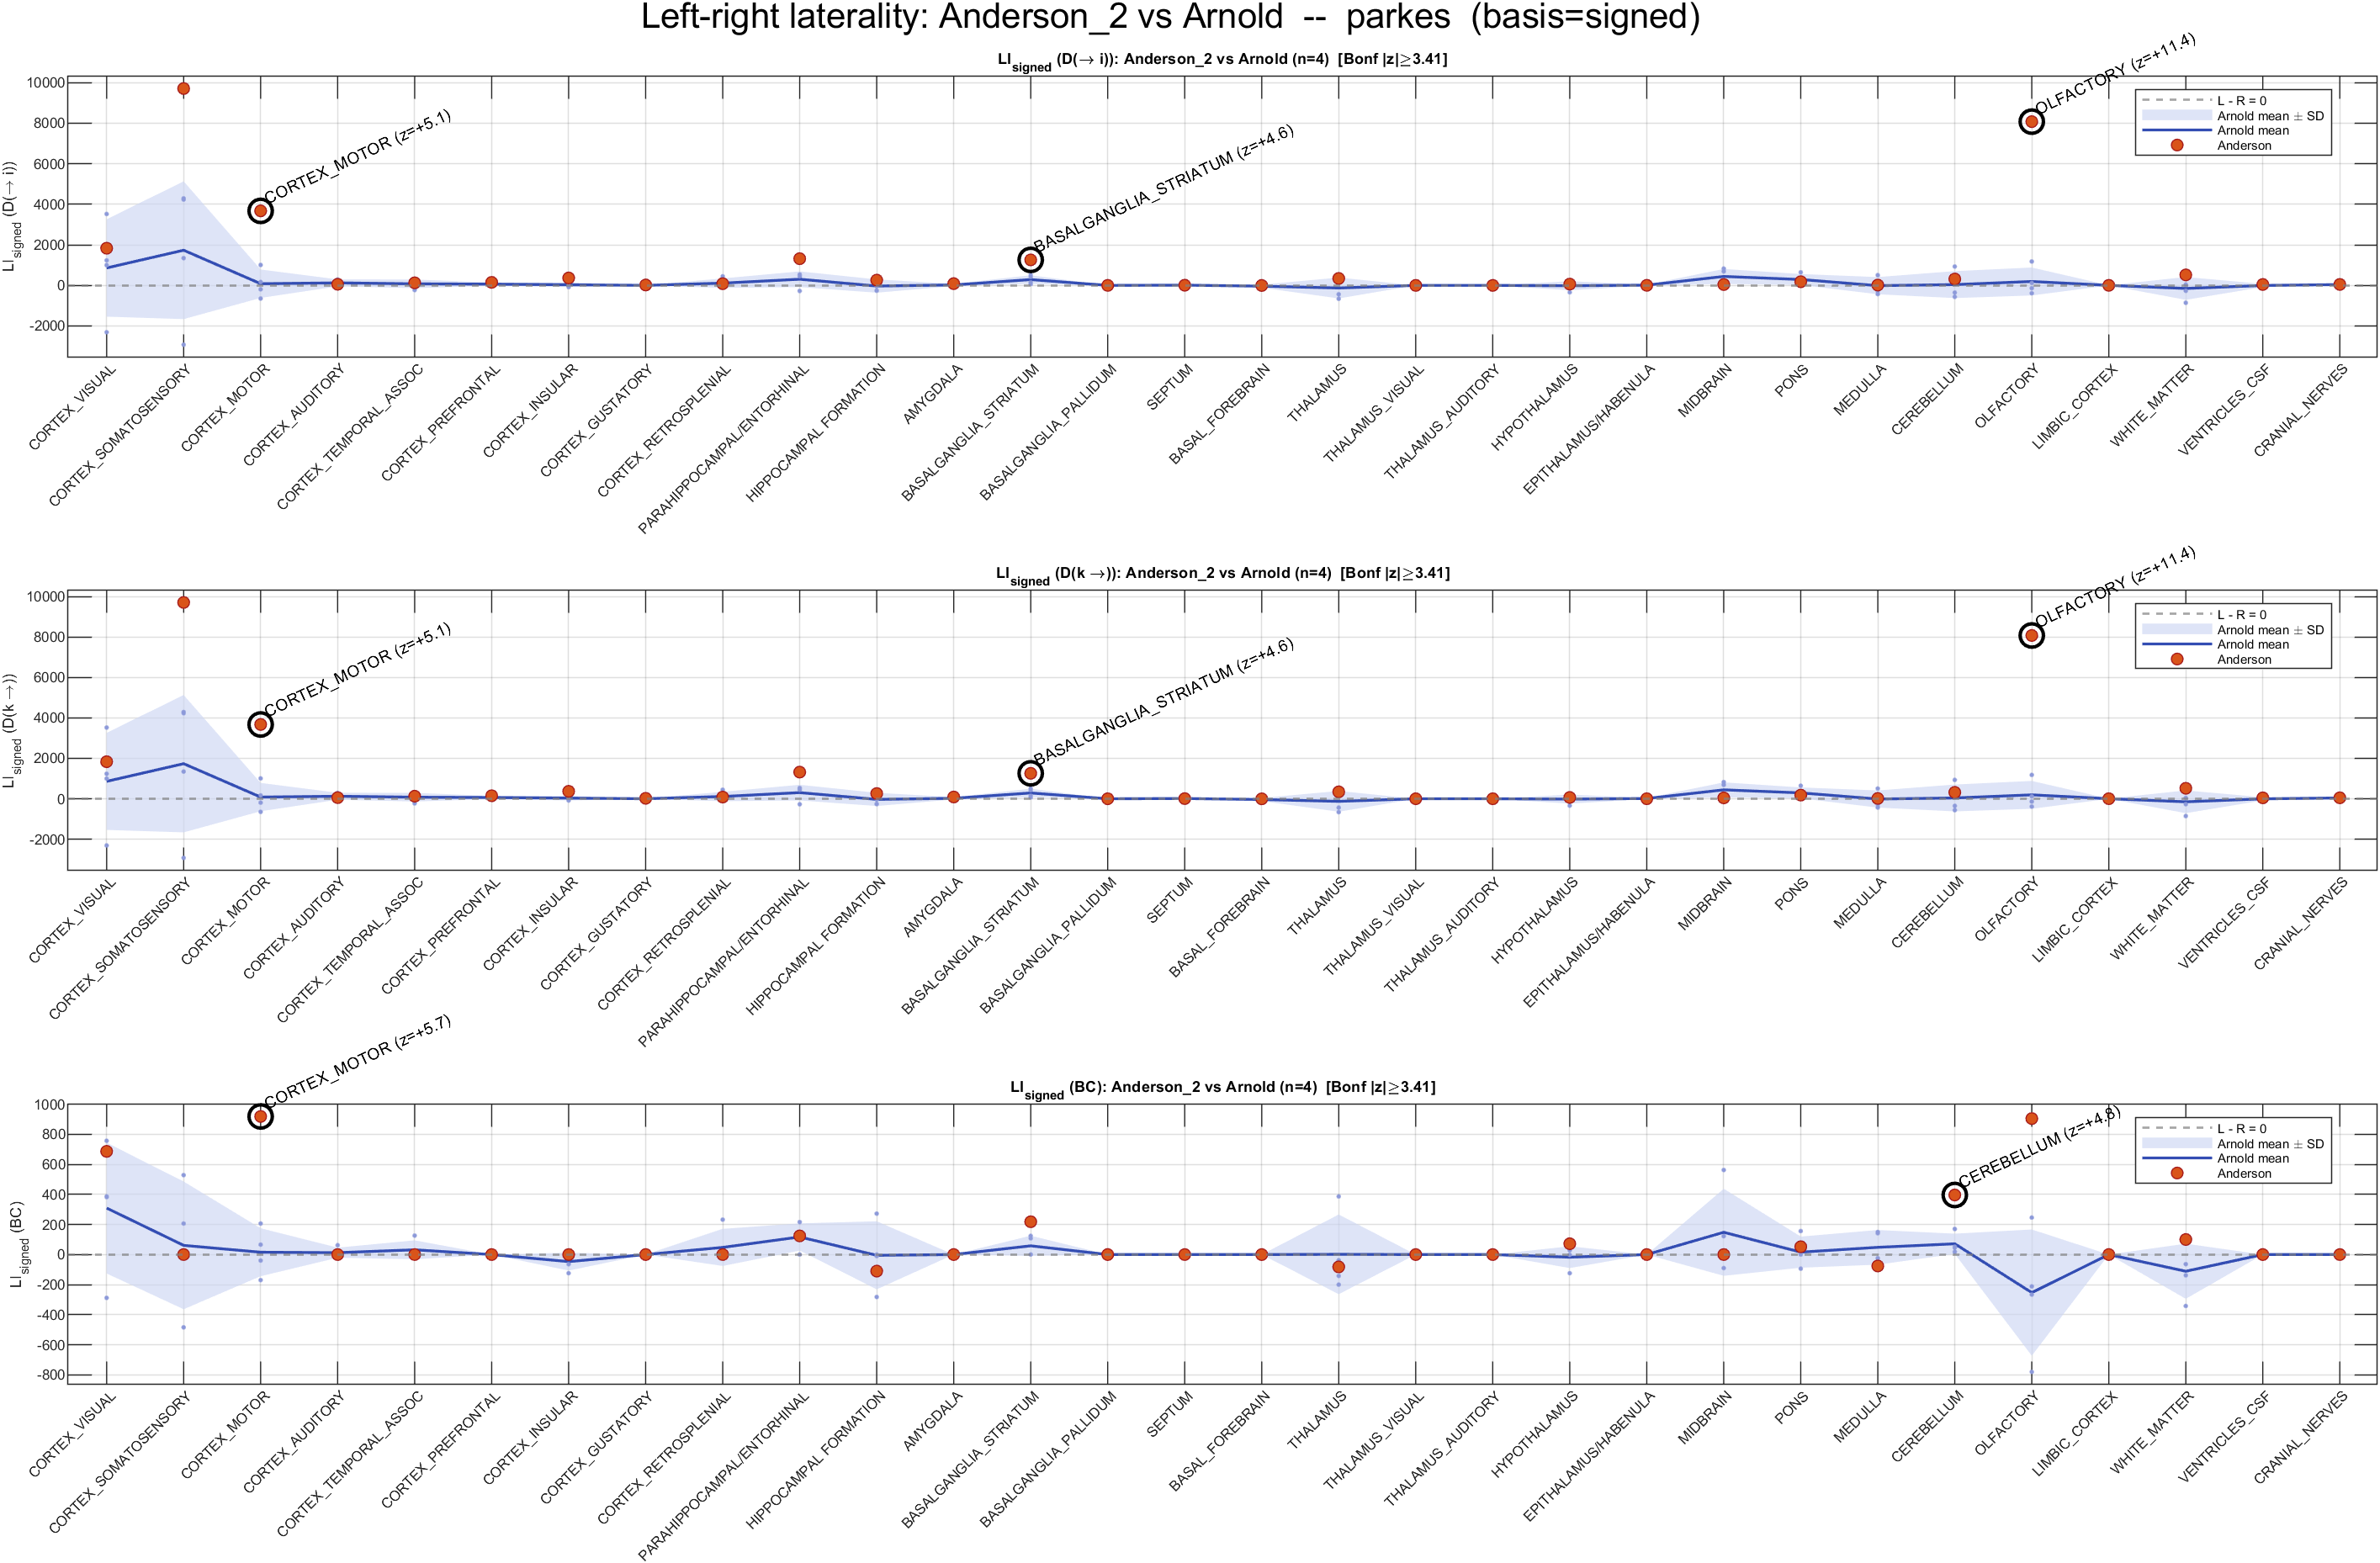
\includegraphics[width=\linewidth]{appendix/compare_LR_asymmetry_Anderson_2_parkes.png}
\caption{\textsc{Anderson\_2}}
\end{subfigure}\hfill
\begin{subfigure}{0.46\textwidth}\centering
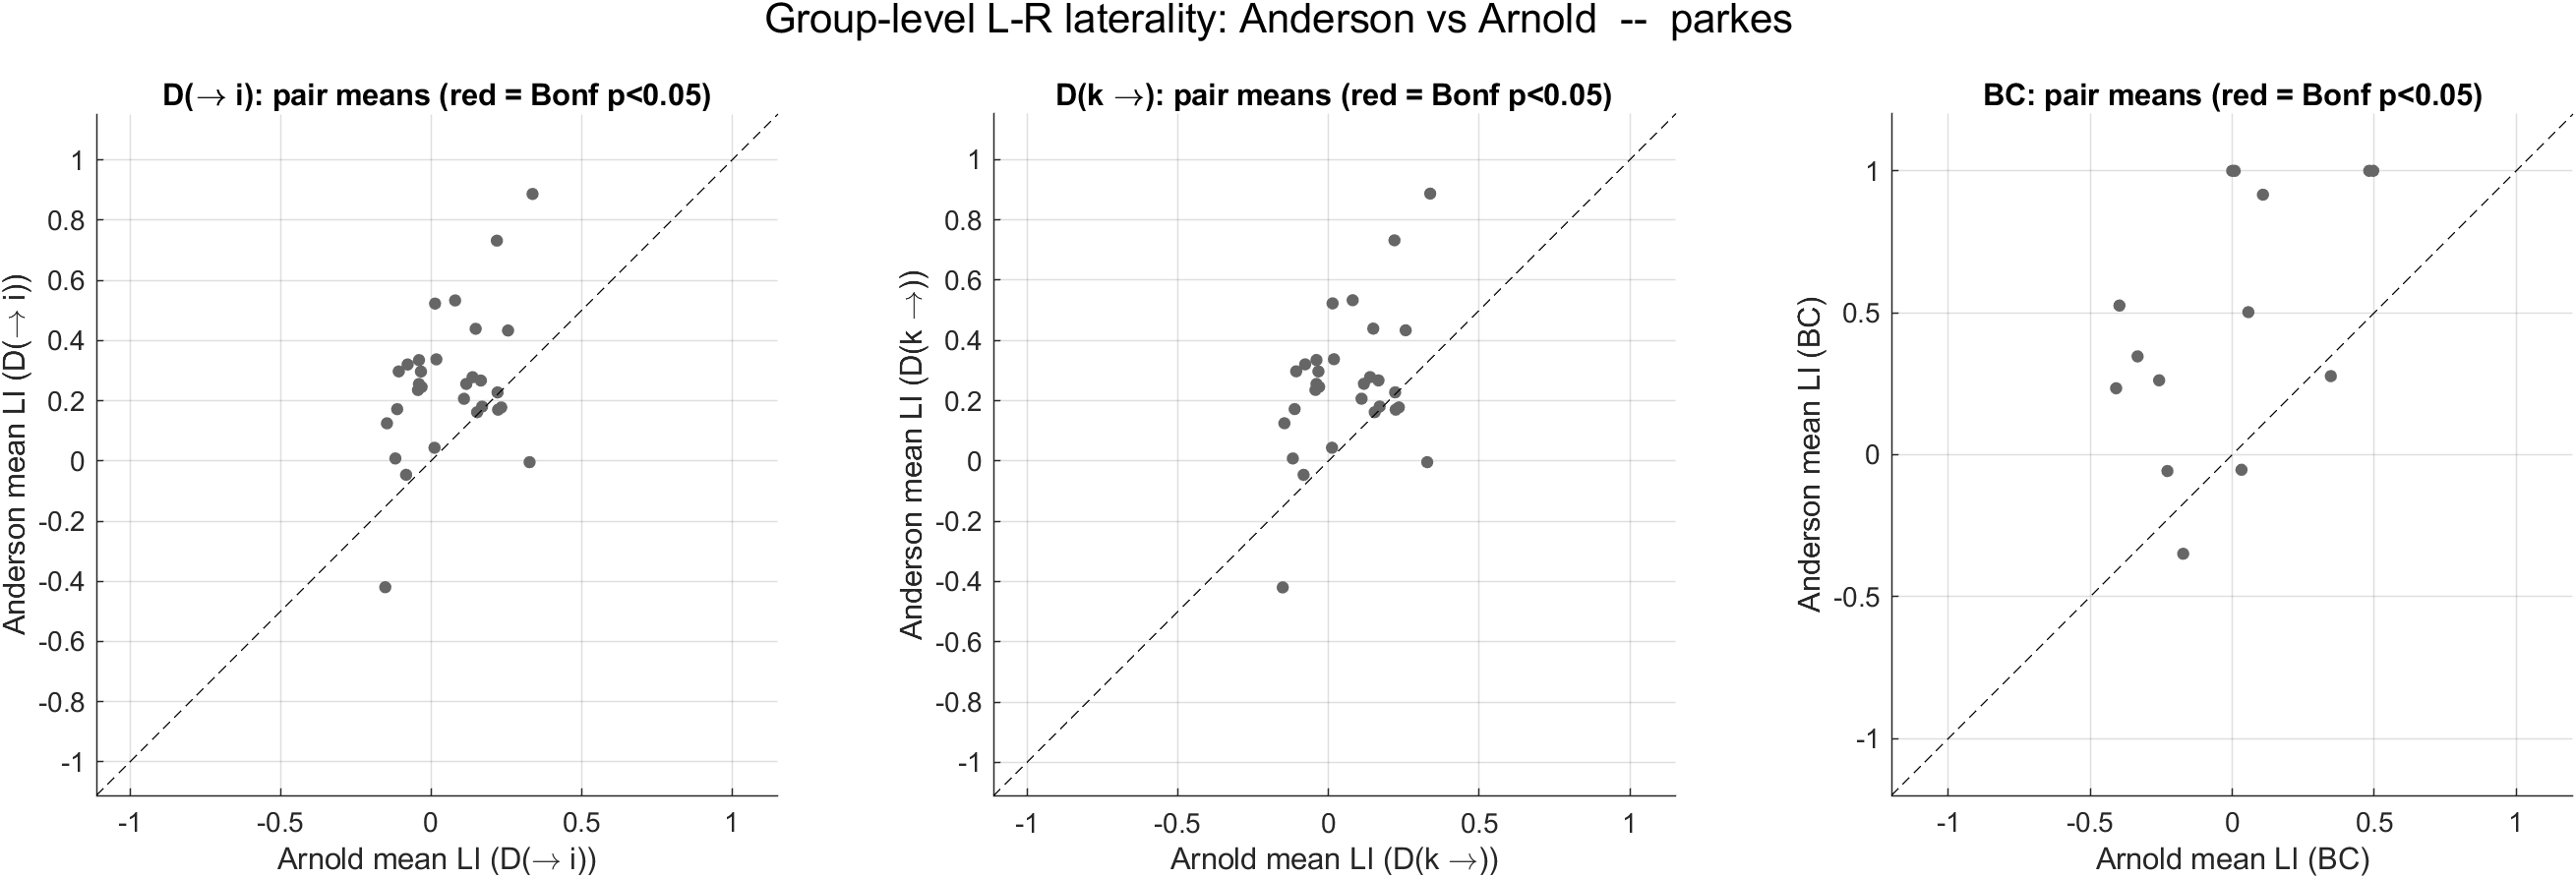
\includegraphics[width=\linewidth]{appendix/LR_asymmetry_groupTest_parkes.png}
\caption{Homotopic-pair group test}
\end{subfigure}\hfill
\begin{subfigure}{0.46\textwidth}\centering
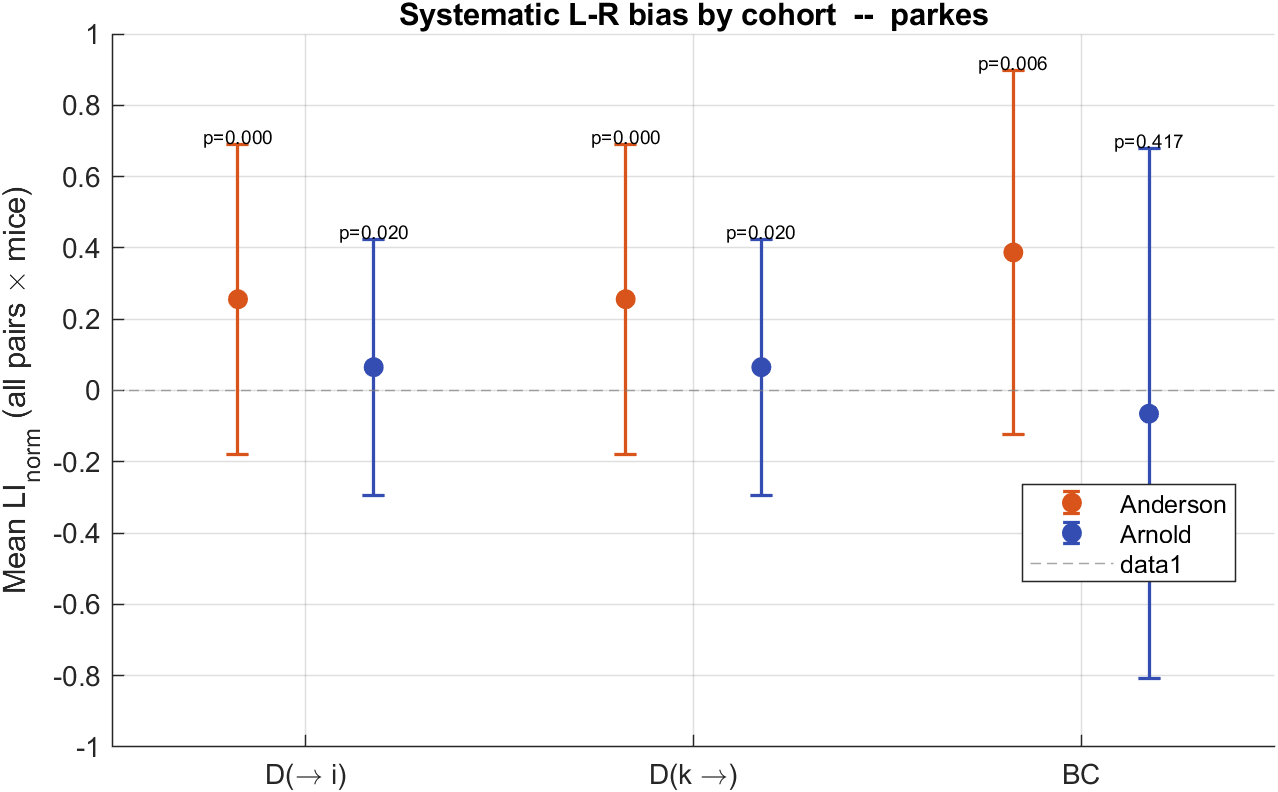
\includegraphics[width=\linewidth]{appendix/LR_asymmetry_systematic_parkes.png}
\caption{Systematic side bias}
\end{subfigure}
\caption{Left--right asymmetry views, \texttt{parkes} scheme.}
\end{figure}

\begin{figure}[H]\centering
\begin{subfigure}{0.46\textwidth}\centering
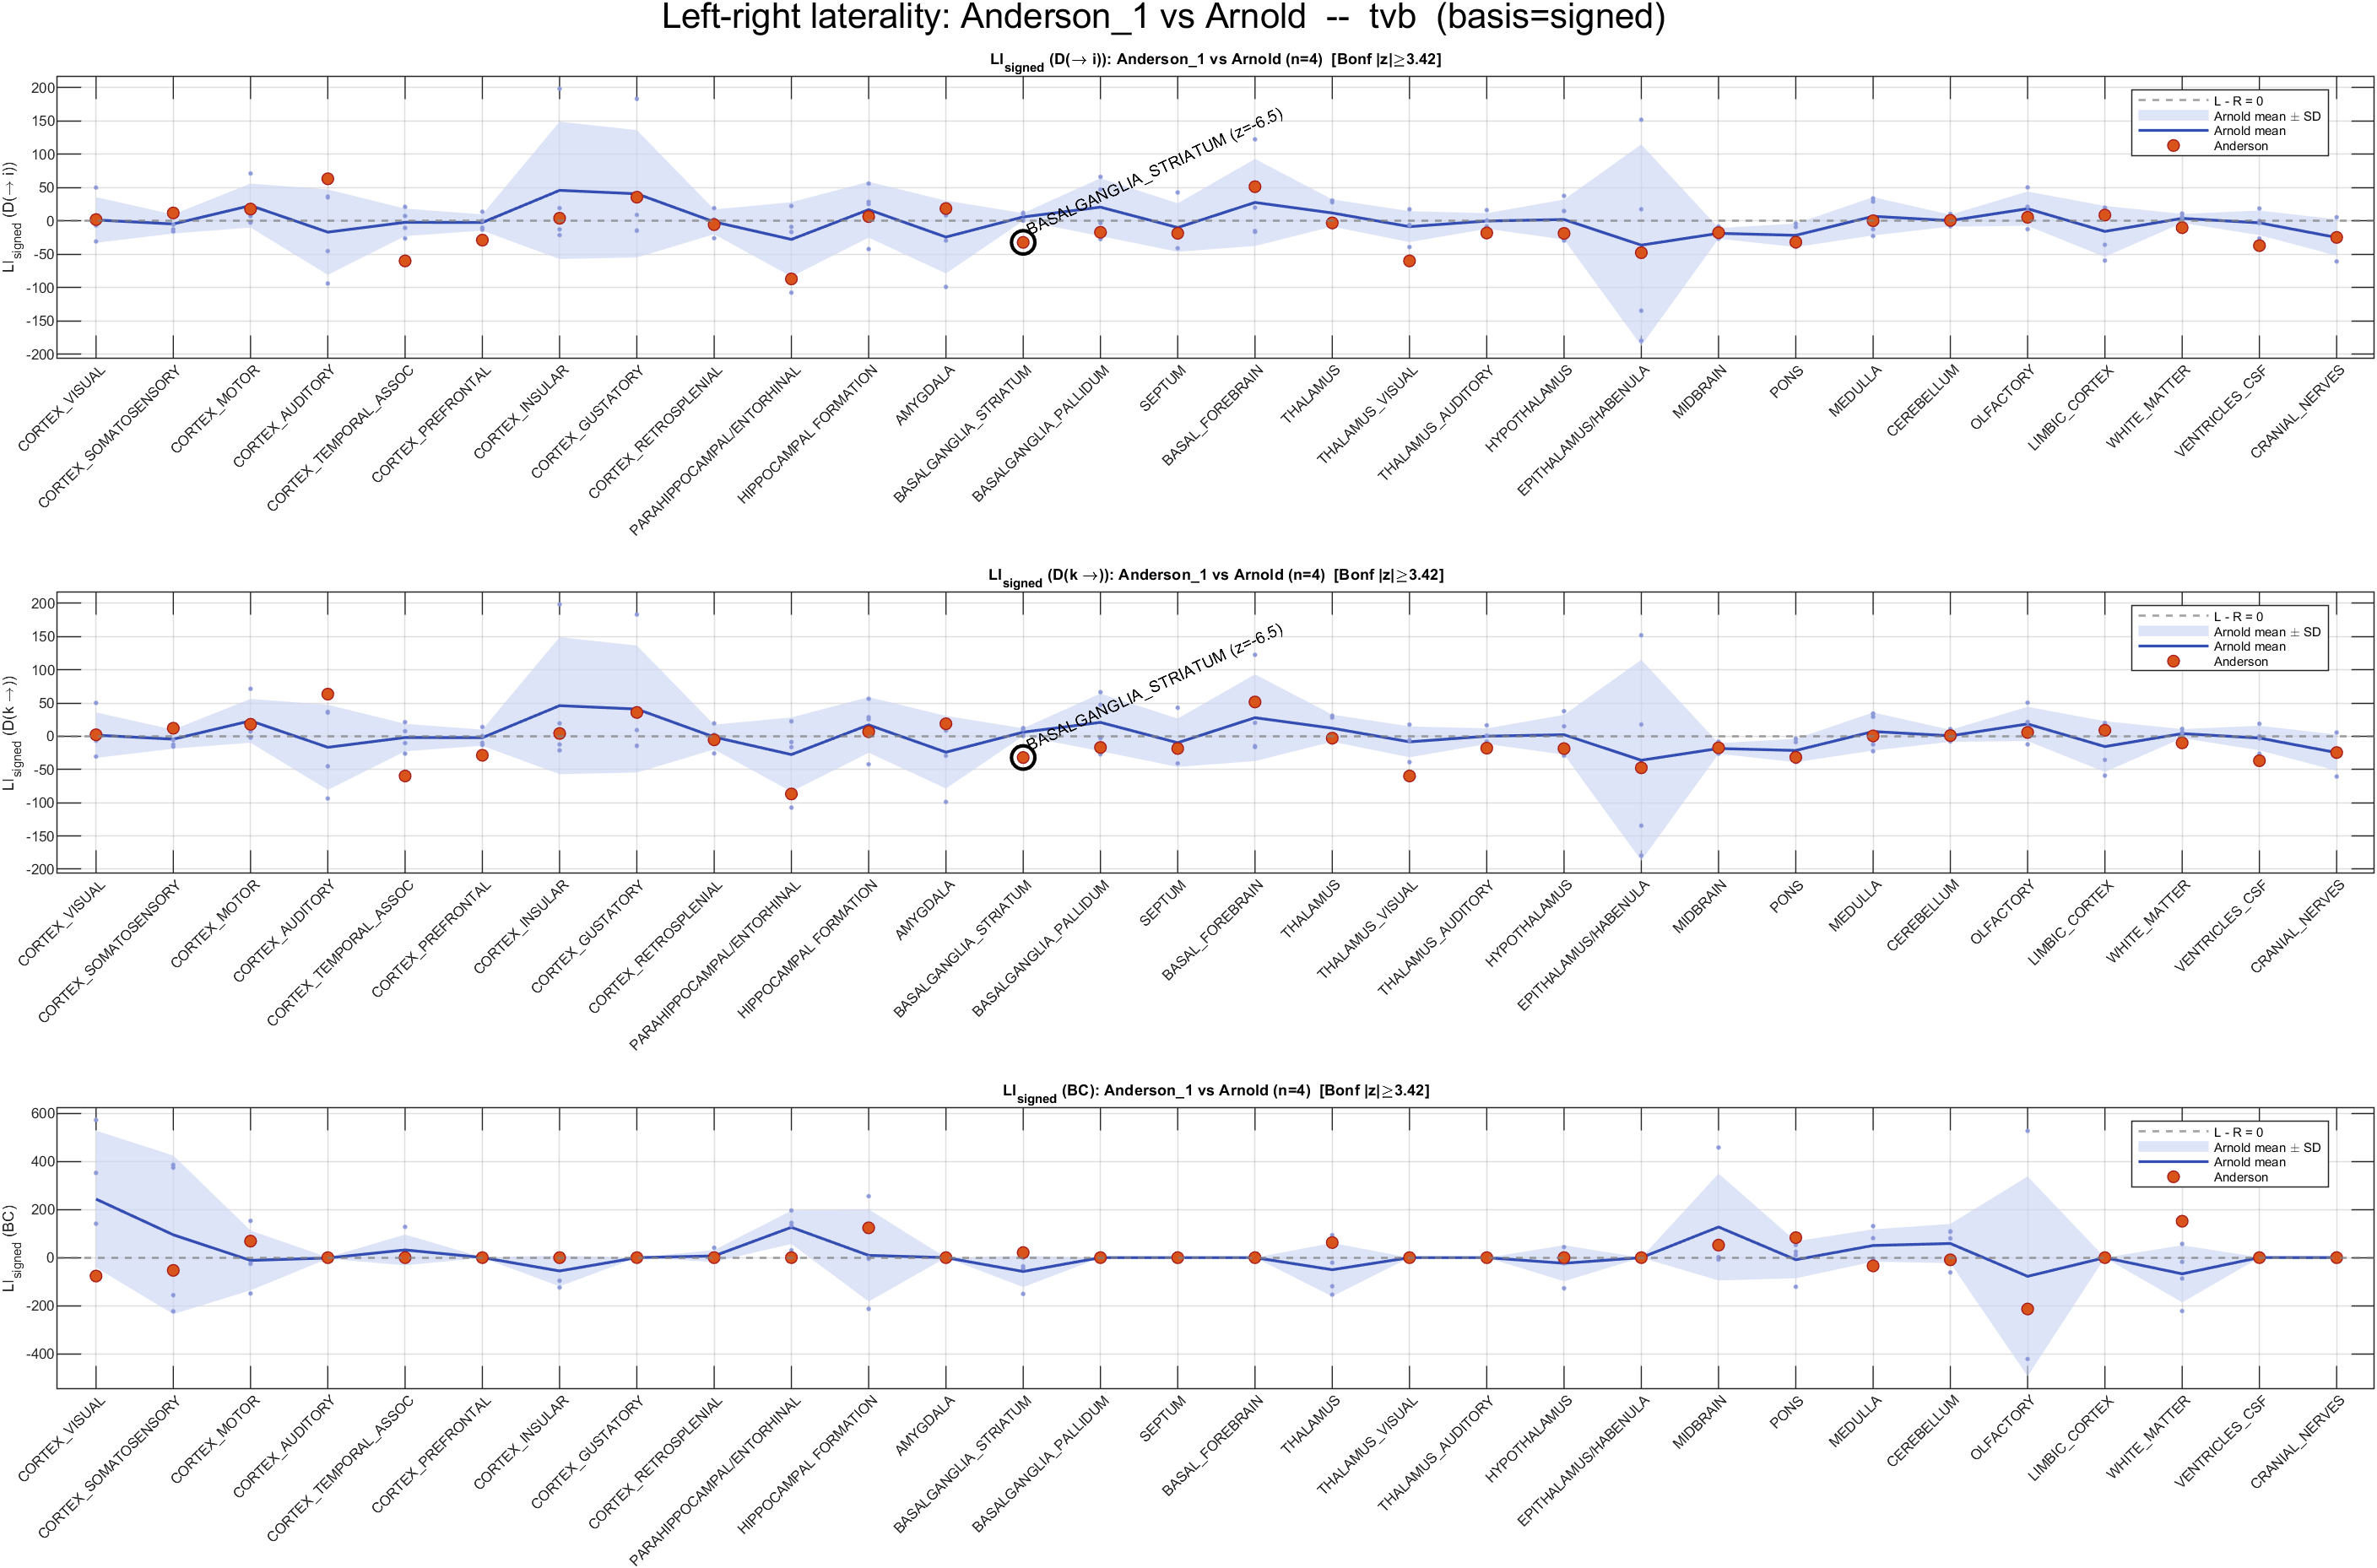
\includegraphics[width=\linewidth]{appendix/compare_LR_asymmetry_Anderson_1_tvb.png}
\caption{\textsc{Anderson\_1}}
\end{subfigure}\hfill
\begin{subfigure}{0.46\textwidth}\centering
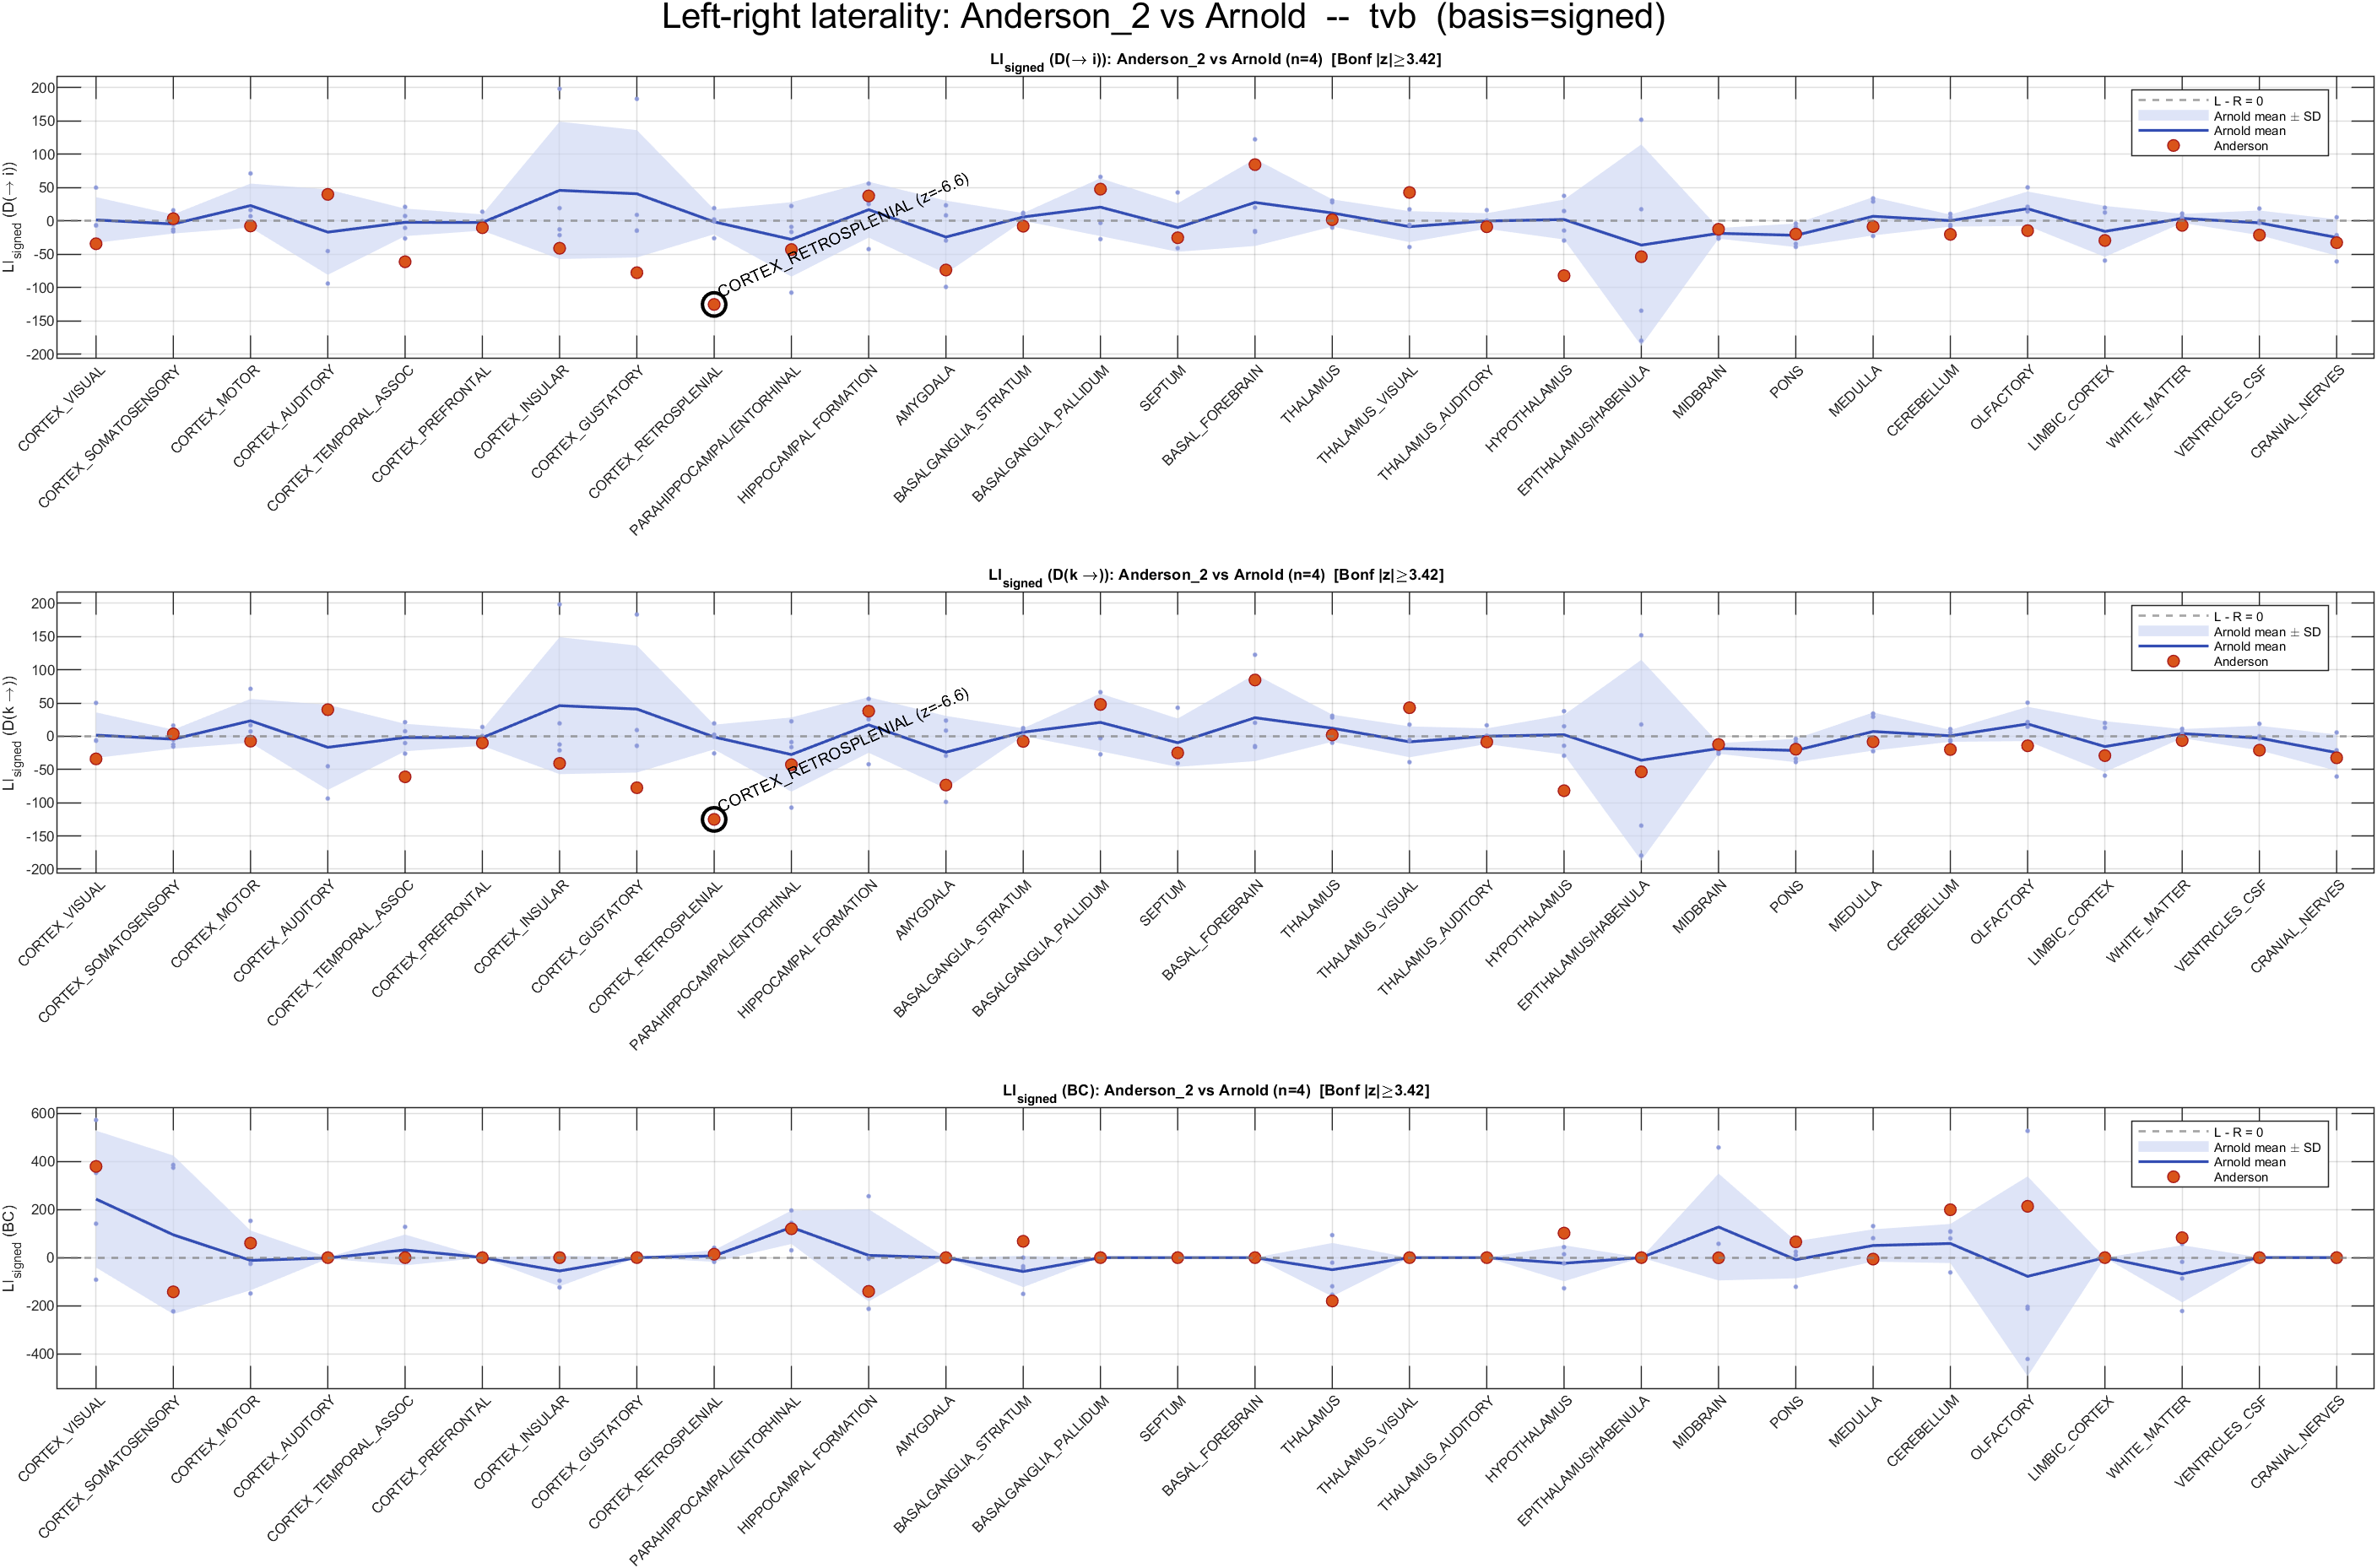
\includegraphics[width=\linewidth]{appendix/compare_LR_asymmetry_Anderson_2_tvb.png}
\caption{\textsc{Anderson\_2}}
\end{subfigure}\hfill
\begin{subfigure}{0.46\textwidth}\centering
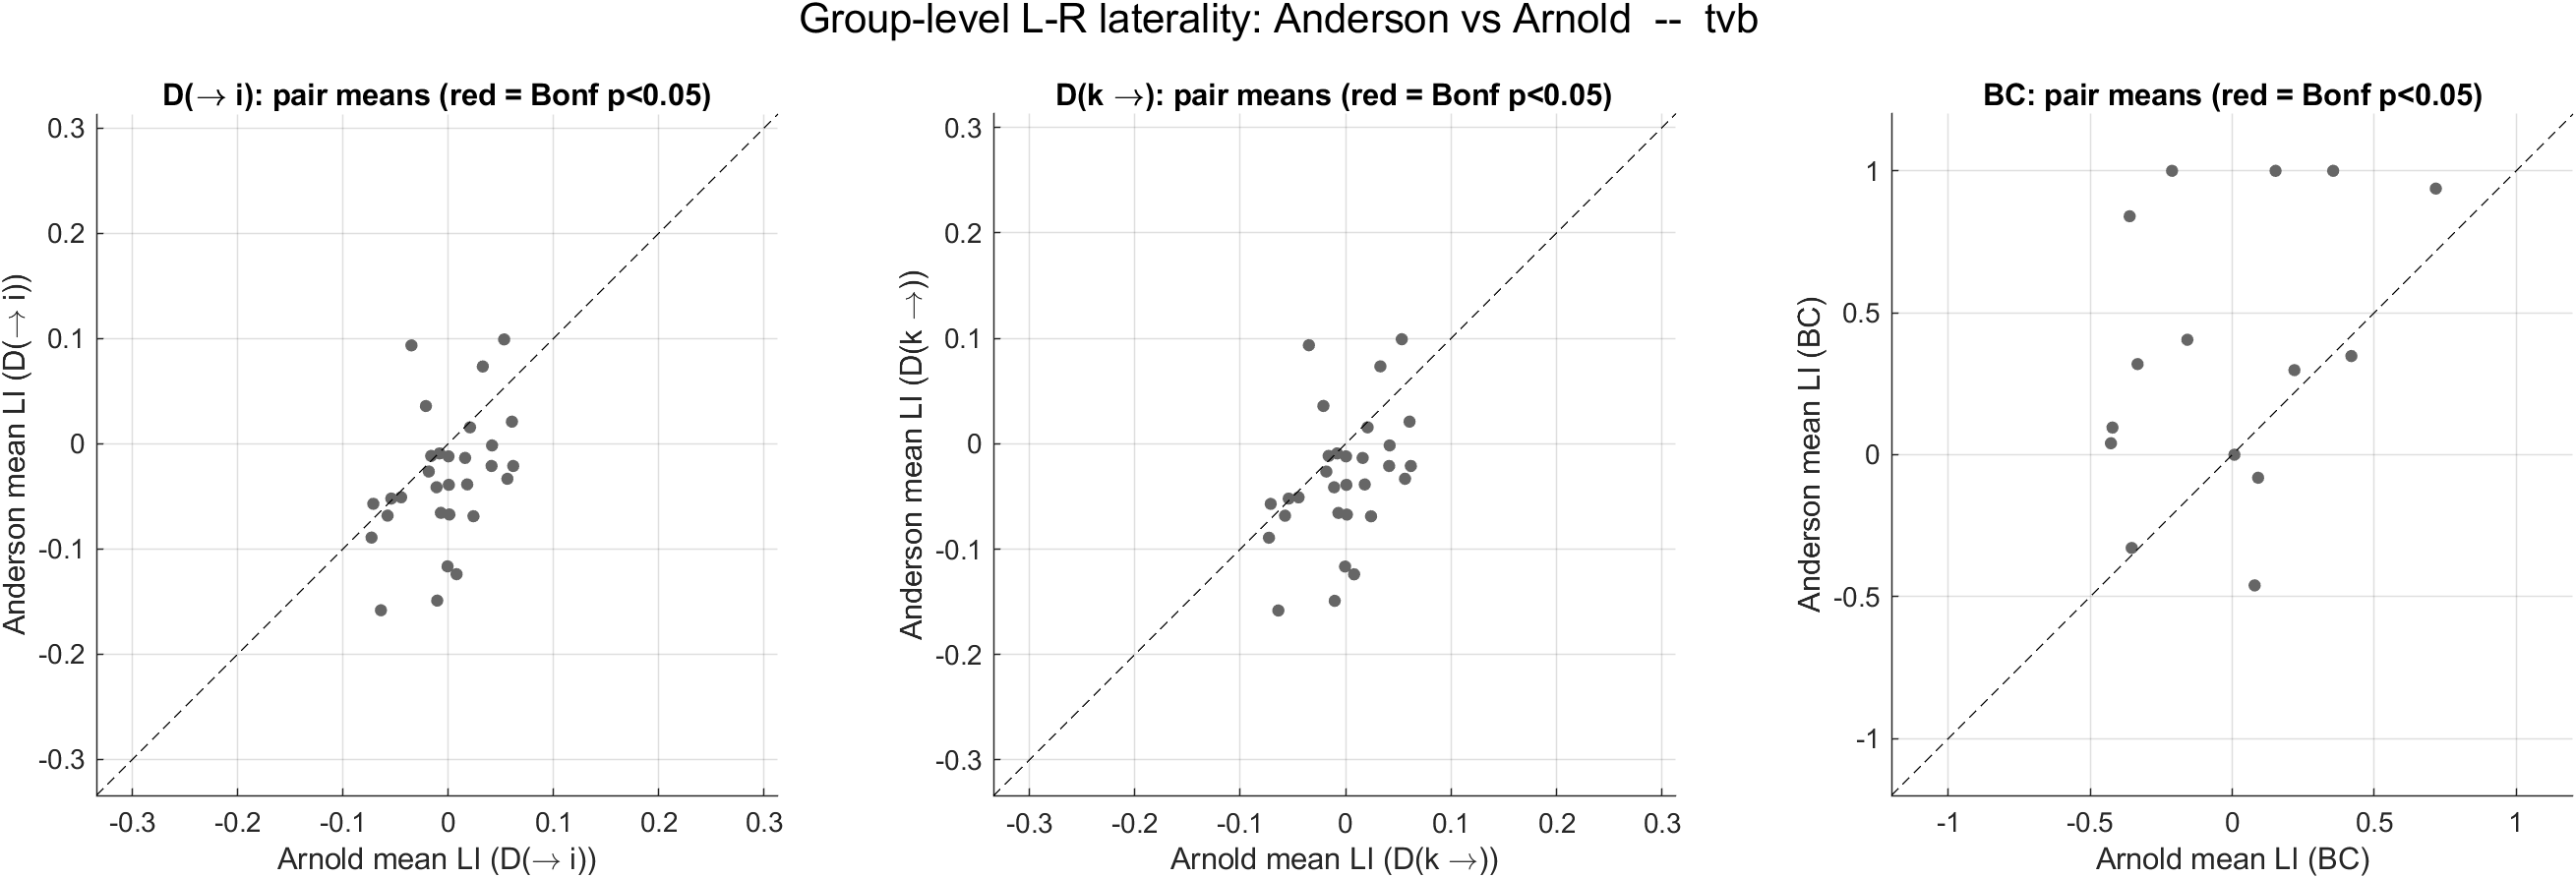
\includegraphics[width=\linewidth]{appendix/LR_asymmetry_groupTest_tvb.png}
\caption{Homotopic-pair group test}
\end{subfigure}\hfill
\begin{subfigure}{0.46\textwidth}\centering
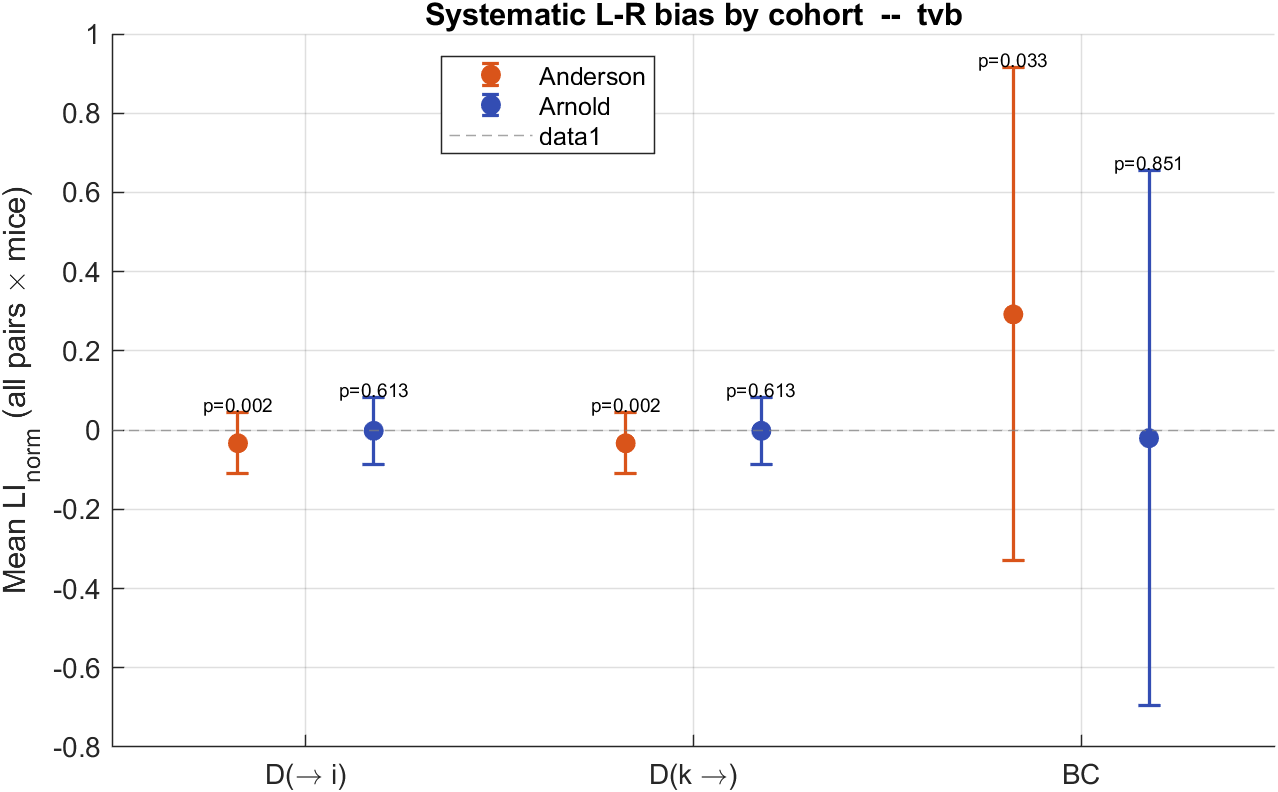
\includegraphics[width=\linewidth]{appendix/LR_asymmetry_systematic_tvb.png}
\caption{Systematic side bias}
\end{subfigure}
\caption{Left--right asymmetry views, \texttt{tvb} scheme.}
\end{figure}

\subsection{Cohort comparison figures (\texttt{column})}
These two summary figures also appear in the main text (Fig.~\ref{fig:outliers}, Fig.~\ref{fig:lr}).
\begin{figure}[H]\centering
\begin{subfigure}{0.49\textwidth}\centering
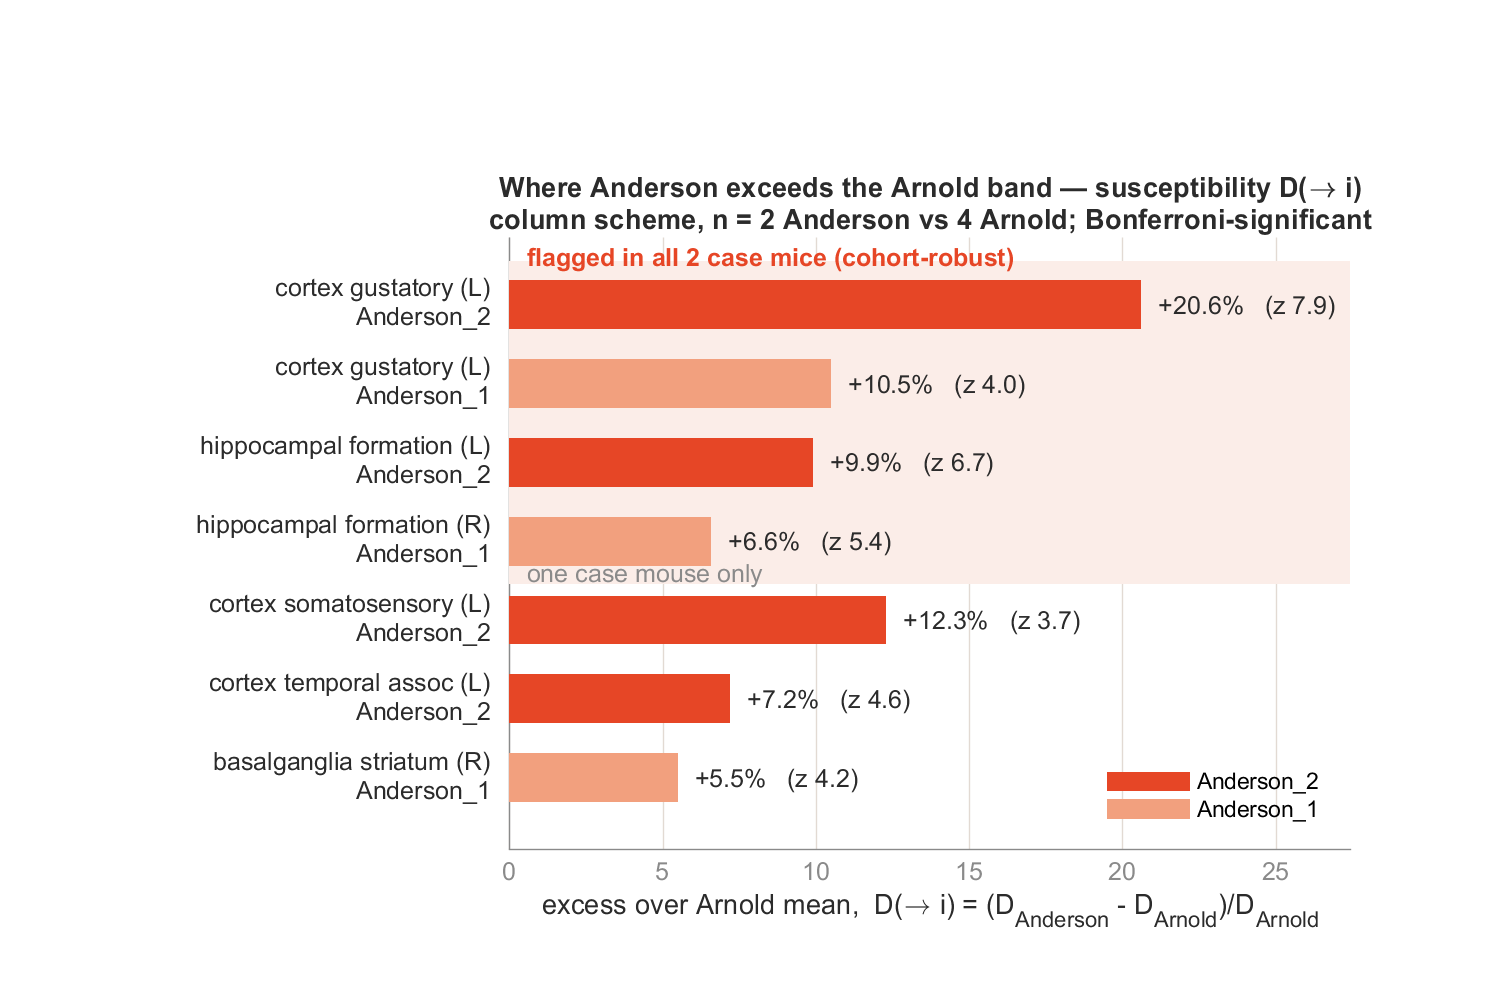
\includegraphics[width=\linewidth]{appendix/region_susc_outliers.png}
\caption{Region susceptibility outliers}
\end{subfigure}\hfill
\begin{subfigure}{0.49\textwidth}\centering
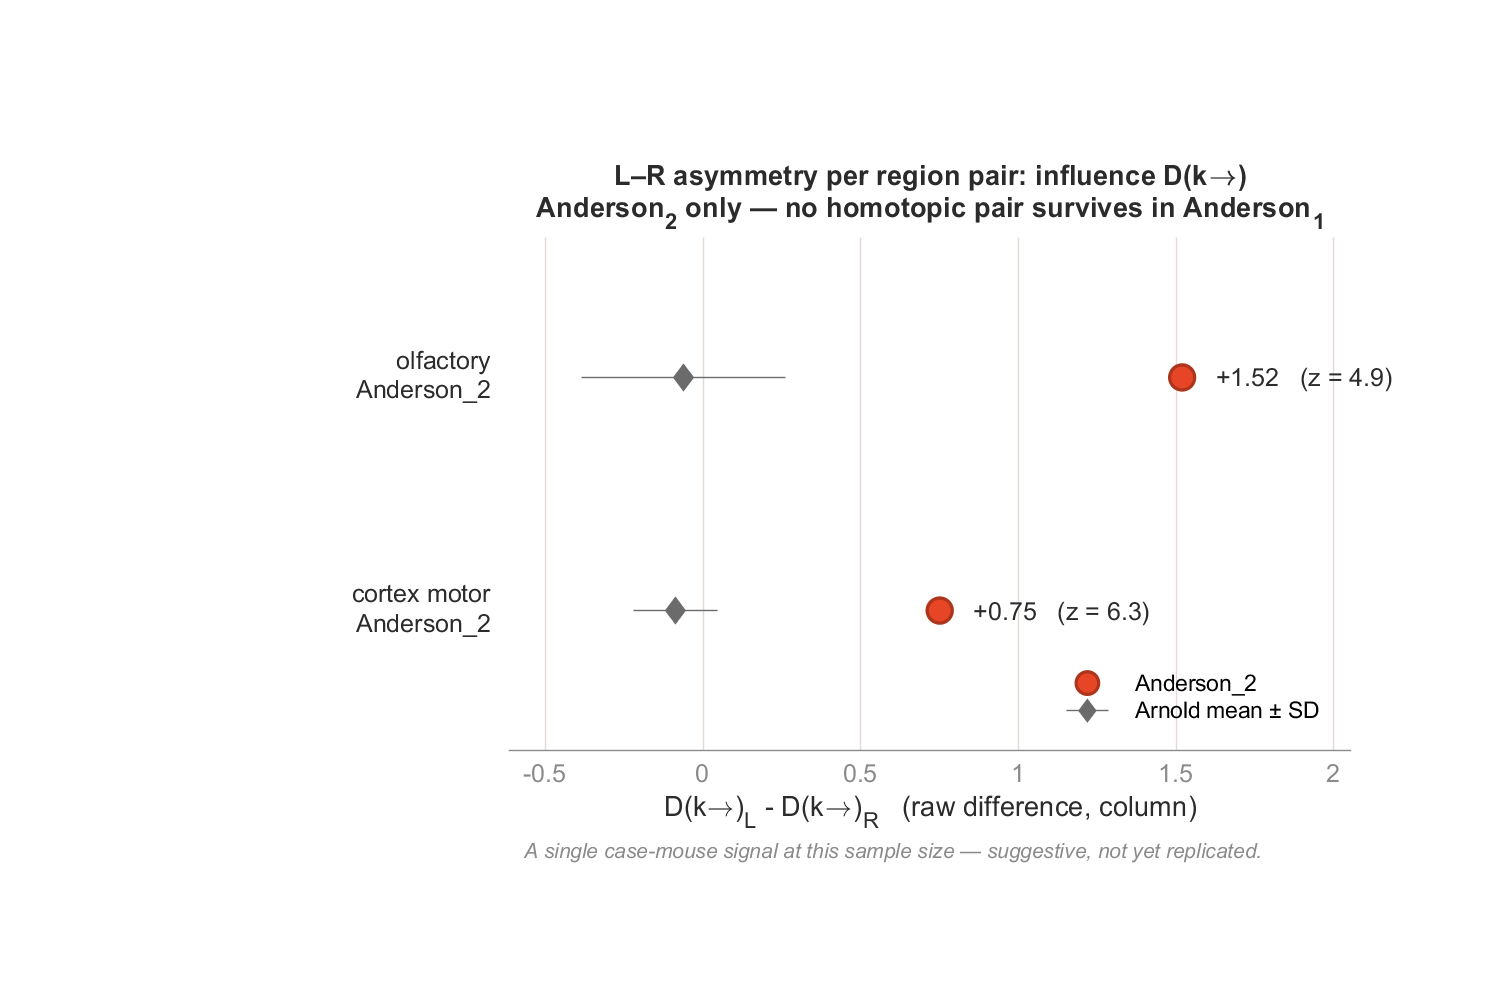
\includegraphics[width=\linewidth]{appendix/laterality_influence_outliers.png}
\caption{Laterality influence outliers}
\end{subfigure}
\caption{Cohort-level Bonferroni-significant outliers, \texttt{column} scheme.}
\end{figure}

\section{Full result tables}
\label{app:tables}
Numeric summaries underlying the figures above. Complete per-node CSVs for every run are written
to the run folders by the pipeline (see Appendix~\ref{app:repro}).

\subsection{Network \texorpdfstring{$\Dst$}{Dst} and spectral radius \texorpdfstring{$\rhoC$}{rho(C)}}
\begin{table}[H]\centering\small
\caption{Per-mouse $\Dst$ and $\rhoC$ for the three schemes. Case mice (\textsc{Anderson}) above the rule.}
\begin{tabular}{@{}l ccc ccc@{}}\toprule
& \multicolumn{3}{c}{$\Dst$} & \multicolumn{3}{c}{$\rhoC$} \\
\cmidrule(lr){2-4}\cmidrule(lr){5-7}
Mouse & \texttt{column} & \texttt{parkes} & \texttt{tvb} & \texttt{column} & \texttt{parkes} & \texttt{tvb} \\\midrule
Anderson\_1 & 0.7924 & 653.3 & 271.9 & 0.95 & 0.999988 & 0.999152 \\
Anderson\_2 & 0.8069 & 545.2 & 274.9 & 0.95 & 0.999986 & 0.999152 \\
\midrule
Arnold\_2 & 0.7582 & 528.9 & 272.1 & 0.95 & 0.999986 & 0.999152 \\
Arnold\_3 & 0.7714 & 643.9 & 272.1 & 0.95 & 0.999988 & 0.999152 \\
Arnold\_4 & 0.7721 & 686.9 & 268.7 & 0.95 & 0.999989 & 0.999152 \\
Arnold\_5 & 0.7884 & 635.8 & 269.5 & 0.95 & 0.999988 & 0.999152 \\
\bottomrule\end{tabular}\end{table}

\subsection{Top regions by stability susceptibility}
\begin{table}[H]\centering\small
\caption{Top 15 non-trivial regions by mean susceptibility rank, \texttt{column} scheme (lower rank = more central).}
\begin{tabular}{@{}rlcc@{}}\toprule
\# & Region & mean rank $\Dto$ & mean rank $\Dfrom$ \\\midrule
1 & L-CORTEX\_SOMATOSENSORY & 3 & 1.67 \\
2 & R-CORTEX\_SOMATOSENSORY & 4.33 & 3.83 \\
3 & L-CEREBELLUM & 5.5 & 8.5 \\
4 & R-CEREBELLUM & 8.17 & 11.2 \\
5 & R-MEDULLA & 9 & 16 \\
6 & L-CORTEX\_VISUAL & 11.3 & 6.83 \\
7 & L-CORTEX\_MOTOR & 12 & 14.7 \\
8 & R-THALAMUS & 12 & 10.8 \\
9 & L-MEDULLA & 14.3 & 20.3 \\
10 & L-OLFACTORY & 14.5 & 9.33 \\
11 & L-PARAHIPPOCAMPAL/ENTORHINAL & 15 & 16.5 \\
12 & R-CORTEX\_VISUAL & 15.5 & 9.67 \\
13 & L-BASALGANGLIA\_STRIATUM & 16.2 & 12.7 \\
14 & R-OLFACTORY & 16.5 & 7.33 \\
15 & R-CORTEX\_MOTOR & 16.7 & 13.3 \\
\bottomrule\end{tabular}\end{table}
\begin{table}[H]\centering\small
\caption{Top 15 non-trivial regions by mean susceptibility rank, \texttt{parkes} scheme (lower rank = more central).}
\begin{tabular}{@{}rlcc@{}}\toprule
\# & Region & mean rank $\Dto$ & mean rank $\Dfrom$ \\\midrule
1 & L-CORTEX\_SOMATOSENSORY & 2.17 & 2.17 \\
2 & R-CORTEX\_SOMATOSENSORY & 4.67 & 4.67 \\
3 & L-CORTEX\_VISUAL & 8.33 & 8.33 \\
4 & L-OLFACTORY & 8.67 & 8.67 \\
5 & R-OLFACTORY & 8.83 & 8.83 \\
6 & L-WHITE\_MATTER & 9.17 & 9.17 \\
7 & L-BASALGANGLIA\_STRIATUM & 9.67 & 9.67 \\
8 & R-WHITE\_MATTER & 10.5 & 10.5 \\
9 & L-CORTEX\_MOTOR & 11.3 & 11.3 \\
10 & R-CORTEX\_VISUAL & 11.5 & 11.5 \\
11 & L-CEREBELLUM & 13 & 13 \\
12 & R-THALAMUS & 13 & 13 \\
13 & R-BASALGANGLIA\_STRIATUM & 13.2 & 13.2 \\
14 & R-CEREBELLUM & 13.8 & 13.8 \\
15 & L-PARAHIPPOCAMPAL/ENTORHINAL & 14 & 14 \\
\bottomrule\end{tabular}\end{table}
\begin{table}[H]\centering\small
\caption{Top 15 non-trivial regions by mean susceptibility rank, \texttt{tvb} scheme (lower rank = more central).}
\begin{tabular}{@{}rlccc@{}}\toprule
\# & Region & mean rank $\Dto$ & mean rank $\Dfrom$ & mean rank $\xcrit$ \\\midrule
1 & R-THALAMUS\_AUDITORY & 5.17 & 5.17 & 1.83 \\
2 & L-THALAMUS\_AUDITORY & 5.67 & 5.67 & 2.17 \\
3 & L-BASALGANGLIA\_PALLIDUM & 9 & 9 & 4.83 \\
4 & R-THALAMUS\_VISUAL & 9.67 & 9.67 & 5.67 \\
5 & R-BASALGANGLIA\_PALLIDUM & 10 & 10 & 6.17 \\
6 & L-THALAMUS\_VISUAL & 10.7 & 10.7 & 6.33 \\
7 & R-EPITHALAMUS/HABENULA & 11.8 & 11.8 & 7.5 \\
8 & R-LIMBIC\_CORTEX & 12.2 & 12.2 & 7.83 \\
9 & L-LIMBIC\_CORTEX & 12.8 & 12.8 & 8.33 \\
10 & L-EPITHALAMUS/HABENULA & 13.7 & 13.7 & 9.17 \\
11 & L-CORTEX\_GUSTATORY & 15.8 & 15.8 & 11.2 \\
12 & R-CORTEX\_GUSTATORY & 17 & 17 & 12.2 \\
13 & R-SEPTUM & 17.5 & 17.5 & 12.5 \\
14 & L-SEPTUM & 19.3 & 19.3 & 14.2 \\
15 & L-BASAL\_FOREBRAIN & 20.8 & 20.8 & 15 \\
\bottomrule\end{tabular}\end{table}

\subsection{Anderson vs Arnold per-region outliers}
\begin{table}[H]\centering\small
\caption{Flagged per-region contrasts ($|z|\ge2$) vs the control band, \texttt{column} scheme. $p_b$ = Bonferroni-corrected $p$; $^{\ast}$ marks significance at $\alpha=0.05$.}
\begin{tabular}{@{}llrrrrrr@{}}\toprule
Mouse & Region & $z_{\mathrm{susc}}$ & $p_b^{\mathrm{susc}}$ & $z_{\mathrm{infl}}$ & $p_b^{\mathrm{infl}}$ & $z_{\mathrm{BC}}$ & $p_b^{\mathrm{BC}}$ \\\midrule
Anderson\_1 & R-CRANIAL\_NERVES & 1.12 & 1 & -0.24 & 1 & 119.50 & $<\!10^{-15}$\textsuperscript{$\ast$} \\
Anderson\_1 & L-CRANIAL\_NERVES & 0.51 & 1 & -0.17 & 1 & 7.17 & $1.3\!\times\!10^{-10}$\textsuperscript{$\ast$} \\
Anderson\_1 & R-THALAMUS & -1.04 & 1 & -0.70 & 1 & 5.65 & $2.8\!\times\!10^{-6}$\textsuperscript{$\ast$} \\
Anderson\_1 & R-HIPPOCAMPAL FORMATION & 5.38 & $1.3\!\times\!10^{-5}$\textsuperscript{$\ast$} & 0.90 & 1 & -0.66 & 1 \\
Anderson\_1 & L-THALAMUS\_VISUAL & 0.35 & 1 & 4.42 & 0.00172\textsuperscript{$\ast$} & 1.50 & 1 \\
Anderson\_1 & R-BASALGANGLIA\_STRIATUM & 4.25 & 0.00379\textsuperscript{$\ast$} & -0.90 & 1 & -0.69 & 1 \\
Anderson\_1 & L-CORTEX\_GUSTATORY & 4.00 & 0.0111\textsuperscript{$\ast$} & -0.32 & 1 & -0.50 & 1 \\
Anderson\_2 & L-CRANIAL\_NERVES & 1.88 & 1 & -0.86 & 1 & 29.42 & $<\!10^{-15}$\textsuperscript{$\ast$} \\
Anderson\_2 & R-VENTRICLES\_CSF & 1.33 & 1 & -2.32 & 1 & 10.77 & $<\!10^{-15}$\textsuperscript{$\ast$} \\
Anderson\_2 & L-CORTEX\_GUSTATORY & 7.87 & $6.3\!\times\!10^{-13}$\textsuperscript{$\ast$} & 0.12 & 1 & -0.50 & 1 \\
Anderson\_2 & L-HIPPOCAMPAL FORMATION & 6.75 & $2.7\!\times\!10^{-9}$\textsuperscript{$\ast$} & 0.53 & 1 & 1.29 & 1 \\
Anderson\_2 & R-THALAMUS & -0.15 & 1 & -0.12 & 1 & 4.80 & $2.9\!\times\!10^{-4}$\textsuperscript{$\ast$} \\
Anderson\_2 & L-CORTEX\_TEMPORAL\_ASSOC & 4.57 & $8.8\!\times\!10^{-4}$\textsuperscript{$\ast$} & -0.91 & 1 & -0.70 & 1 \\
Anderson\_2 & L-CORTEX\_SOMATOSENSORY & 3.74 & 0.033\textsuperscript{$\ast$} & 1.31 & 1 & 0.07 & 1 \\
Anderson\_2 & L-WHITE\_MATTER & 3.03 & 0.433 & 0.77 & 1 & 3.65 & 0.0469\textsuperscript{$\ast$} \\
\bottomrule\end{tabular}\end{table}
\begin{table}[H]\centering\small
\caption{Flagged per-region contrasts ($|z|\ge2$) vs the control band, \texttt{parkes} scheme. $p_b$ = Bonferroni-corrected $p$; $^{\ast}$ marks significance at $\alpha=0.05$.}
\begin{tabular}{@{}llrrrrrr@{}}\toprule
Mouse & Region & $z_{\mathrm{susc}}$ & $p_b^{\mathrm{susc}}$ & $z_{\mathrm{infl}}$ & $p_b^{\mathrm{infl}}$ & $z_{\mathrm{BC}}$ & $p_b^{\mathrm{BC}}$ \\\midrule
Anderson\_1 & R-AMYGDALA & 7.40 & $2.2\!\times\!10^{-11}$\textsuperscript{$\ast$} & 7.40 & $2.2\!\times\!10^{-11}$\textsuperscript{$\ast$} & -- & 1 \\
Anderson\_1 & L-THALAMUS\_VISUAL & 3.86 & 0.0174\textsuperscript{$\ast$} & 3.86 & 0.0174\textsuperscript{$\ast$} & -- & 1 \\
Anderson\_2 & R-THALAMUS & -7.45 & $1.5\!\times\!10^{-11}$\textsuperscript{$\ast$} & -7.45 & $1.5\!\times\!10^{-11}$\textsuperscript{$\ast$} & 2.10 & 1 \\
Anderson\_2 & L-CORTEX\_MOTOR & 3.51 & 0.0692 & 3.51 & 0.0692 & 7.43 & $1.7\!\times\!10^{-11}$\textsuperscript{$\ast$} \\
\bottomrule\end{tabular}\end{table}
\begin{table}[H]\centering\small
\caption{Flagged per-region contrasts ($|z|\ge2$) vs the control band, \texttt{tvb} scheme. $p_b$ = Bonferroni-corrected $p$; $^{\ast}$ marks significance at $\alpha=0.05$.}
\begin{tabular}{@{}llrrrrrr@{}}\toprule
Mouse & Region & $z_{\mathrm{susc}}$ & $p_b^{\mathrm{susc}}$ & $z_{\mathrm{infl}}$ & $p_b^{\mathrm{infl}}$ & $z_{\mathrm{BC}}$ & $p_b^{\mathrm{BC}}$ \\\midrule
Anderson\_1 & R-MEDULLA & -0.67 & 1 & -0.67 & 1 & 6.78 & $1.8\!\times\!10^{-9}$\textsuperscript{$\ast$} \\
Anderson\_1 & R-WHITE\_MATTER & 4.15 & 0.00527\textsuperscript{$\ast$} & 4.15 & 0.00527\textsuperscript{$\ast$} & -1.01 & 1 \\
Anderson\_1 & L-THALAMUS\_VISUAL & -3.98 & 0.011\textsuperscript{$\ast$} & -3.98 & 0.011\textsuperscript{$\ast$} & -- & 1 \\
Anderson\_2 & R-CORTEX\_GUSTATORY & 7.29 & $4.9\!\times\!10^{-11}$\textsuperscript{$\ast$} & 7.29 & $4.9\!\times\!10^{-11}$\textsuperscript{$\ast$} & -- & 1 \\
Anderson\_2 & R-CORTEX\_MOTOR & -0.79 & 1 & -0.79 & 1 & 3.70 & 0.0345\textsuperscript{$\ast$} \\
\bottomrule\end{tabular}\end{table}

\subsection{Systematic laterality}
\begin{table}[H]\centering\small
\caption{Cohort-wide sign-rank test of the normalised laterality index $\mathrm{LI}_{\mathrm{norm}}$ against zero, all schemes. Side = inferred dominant hemisphere (nominal labels).}
\begin{tabular}{@{}lllrrrl@{}}\toprule
Scheme & Cohort & Metric & mean LI & sd LI & sign-rank $p$ & Side \\\midrule
\texttt{column} & Anderson & D\_susc & 0.00879 & 0.0188 & $7.9\!\times\!10^{-4}$ & L \\
\texttt{column} & Arnold & D\_susc & 0.00173 & 0.0131 & 0.0724 & none \\
\texttt{column} & Anderson & D\_infl & 0.0399 & 0.0982 & 0.0026 & L \\
\texttt{column} & Arnold & D\_infl & 0.00862 & 0.083 & 0.178 & none \\
\texttt{column} & Anderson & BC & 0.156 & 0.694 & 0.189 & none \\
\texttt{column} & Arnold & BC & -0.0734 & 0.668 & 0.291 & none \\
\midrule
\texttt{parkes} & Anderson & D\_susc & 0.256 & 0.435 & $1.0\!\times\!10^{-4}$ & L \\
\texttt{parkes} & Arnold & D\_susc & 0.0654 & 0.359 & 0.0203 & L \\
\texttt{parkes} & Anderson & D\_infl & 0.256 & 0.435 & $1.0\!\times\!10^{-4}$ & L \\
\texttt{parkes} & Arnold & D\_infl & 0.0654 & 0.359 & 0.0203 & L \\
\texttt{parkes} & Anderson & BC & 0.387 & 0.511 & 0.00609 & L \\
\texttt{parkes} & Arnold & BC & -0.0651 & 0.744 & 0.417 & none \\
\midrule
\texttt{tvb} & Anderson & D\_susc & -0.0332 & 0.0769 & 0.00151 & R \\
\texttt{tvb} & Arnold & D\_susc & -0.00186 & 0.0838 & 0.613 & none \\
\texttt{tvb} & Anderson & D\_infl & -0.0332 & 0.0769 & 0.00151 & R \\
\texttt{tvb} & Arnold & D\_infl & -0.00186 & 0.0838 & 0.613 & none \\
\texttt{tvb} & Anderson & BC & 0.292 & 0.622 & 0.033 & L \\
\texttt{tvb} & Arnold & BC & -0.0203 & 0.676 & 0.851 & none \\
\bottomrule\end{tabular}\end{table}

\subsection{Homotopic-pair laterality tests}
\begin{table}[H]\centering\small
\caption{Per-pair Welch $t$-test between strains, \texttt{column} scheme: 10 smallest Bonferroni $p$. $\checkmark$ marks $p_b<0.05$.}
\begin{tabular}{@{}llrrrrc@{}}\toprule
Region & Metric & $\mathrm{LI}_{\mathrm{And}}$ & $\mathrm{LI}_{\mathrm{Arn}}$ & $t$ & $p_b$ & sig. \\\midrule
CORTEX\_VISUAL & D\_susc & 0.016 & 0.00737 & 0.58 & 1 &  \\
CORTEX\_SOMATOSENSORY & D\_susc & 0.0119 & 0.0146 & -0.10 & 1 &  \\
CORTEX\_MOTOR & D\_susc & 0.0261 & -0.000446 & 2.45 & 1 &  \\
CORTEX\_AUDITORY & D\_susc & 0.0213 & 0.0125 & 0.36 & 1 &  \\
CORTEX\_TEMPORAL\_ASSOC & D\_susc & 0.0252 & 0.00942 & 3.27 & 1 &  \\
CORTEX\_PREFRONTAL & D\_susc & 0.00152 & 0.00215 & -0.11 & 1 &  \\
CORTEX\_INSULAR & D\_susc & 0.022 & -0.00112 & 1.01 & 1 &  \\
CORTEX\_GUSTATORY & D\_susc & 0.0486 & -0.00299 & 2.68 & 1 &  \\
CORTEX\_RETROSPLENIAL & D\_susc & 0.00464 & -0.00525 & 1.12 & 1 &  \\
PARAHIPPOCAMPAL/ENTORHINAL & D\_susc & 0.0274 & -0.000259 & 1.46 & 1 &  \\
\bottomrule\end{tabular}\end{table}
\begin{table}[H]\centering\small
\caption{Per-pair Welch $t$-test between strains, \texttt{parkes} scheme: 10 smallest Bonferroni $p$. $\checkmark$ marks $p_b<0.05$.}
\begin{tabular}{@{}llrrrrc@{}}\toprule
Region & Metric & $\mathrm{LI}_{\mathrm{And}}$ & $\mathrm{LI}_{\mathrm{Arn}}$ & $t$ & $p_b$ & sig. \\\midrule
CORTEX\_VISUAL & D\_susc & 0.533 & 0.0803 & 0.98 & 1 &  \\
CORTEX\_SOMATOSENSORY & D\_susc & 0.17 & 0.223 & -0.08 & 1 &  \\
CORTEX\_MOTOR & D\_susc & 0.256 & -0.0398 & 0.51 & 1 &  \\
CORTEX\_AUDITORY & D\_susc & -0.00396 & 0.328 & -0.50 & 1 &  \\
CORTEX\_TEMPORAL\_ASSOC & D\_susc & 0.732 & 0.219 & 1.99 & 1 &  \\
CORTEX\_PREFRONTAL & D\_susc & 0.256 & 0.117 & 1.18 & 1 &  \\
CORTEX\_INSULAR & D\_susc & 0.321 & -0.0774 & 0.57 & 1 &  \\
CORTEX\_GUSTATORY & D\_susc & 0.298 & -0.107 & 0.58 & 1 &  \\
CORTEX\_RETROSPLENIAL & D\_susc & 0.523 & 0.0136 & 1.48 & 1 &  \\
PARAHIPPOCAMPAL/ENTORHINAL & D\_susc & 0.887 & 0.337 & 2.41 & 1 &  \\
\bottomrule\end{tabular}\end{table}
\begin{table}[H]\centering\small
\caption{Per-pair Welch $t$-test between strains, \texttt{tvb} scheme: 10 smallest Bonferroni $p$. $\checkmark$ marks $p_b<0.05$.}
\begin{tabular}{@{}llrrrrc@{}}\toprule
Region & Metric & $\mathrm{LI}_{\mathrm{And}}$ & $\mathrm{LI}_{\mathrm{Arn}}$ & $t$ & $p_b$ & sig. \\\midrule
CORTEX\_VISUAL & D\_susc & -0.0672 & 0.00111 & -0.67 & 1 &  \\
CORTEX\_SOMATOSENSORY & D\_susc & 0.0358 & -0.0212 & 1.45 & 1 &  \\
CORTEX\_MOTOR & D\_susc & 0.021 & 0.0605 & -0.61 & 1 &  \\
CORTEX\_AUDITORY & D\_susc & 0.0934 & -0.0349 & 1.88 & 1 &  \\
CORTEX\_TEMPORAL\_ASSOC & D\_susc & -0.116 & -0.000611 & -4.30 & 1 &  \\
CORTEX\_PREFRONTAL & D\_susc & -0.0413 & -0.011 & -1.61 & 1 &  \\
CORTEX\_INSULAR & D\_susc & -0.0333 & 0.0562 & -1.09 & 1 &  \\
CORTEX\_GUSTATORY & D\_susc & -0.0211 & 0.0412 & -0.76 & 1 &  \\
CORTEX\_RETROSPLENIAL & D\_susc & -0.149 & -0.0104 & -1.04 & 1 &  \\
PARAHIPPOCAMPAL/ENTORHINAL & D\_susc & -0.158 & -0.0639 & -1.12 & 1 &  \\
\bottomrule\end{tabular}\end{table}



\end{document}
